\documentclass[11pt,a4paper]{article}


\usepackage[margin = 1in]{geometry}
\usepackage{amsfonts, amssymb,amsmath}
\usepackage[none]{hyphenat}
\usepackage{fancyhdr}
\usepackage{graphicx}
\usepackage{float}
\usepackage{color}
\usepackage{tikz}
\usepackage{polynom}
\usepackage[nottoc, notlot, notlof]{tocbibind}
\usepackage{bigints}
\usepackage{xcolor}
\usepackage{esint}

% ---------------------------------------------------------------------------
% Additions for the web build. Nothing below changes the printed page.
%
% enumitem preserves the optional label on \item[(a).]. Without it tex4ht
% discards the label and numbers the list itself, so a question whose parts
% are (i), (ii), (iii) comes out lettered a, b, c and any prose referring to
% "the integral in (ii)" points at the wrong item.
% ---------------------------------------------------------------------------
\usepackage{enumitem}
\usepackage{amsthm}
\theoremstyle{definition}
\newtheorem{thm}{Theorem}[section]
\newtheorem{definition}[thm]{Definition}
\newtheorem{example}[thm]{Example}
\newtheorem{exe}[thm]{Exercise}
\newtheorem{note}[thm]{Note}
\newtheorem{remark}[thm]{Remark}
% Unlike the other courses, `problem` takes no argument here: this is a
% fourth-year course and its readers do not need to be told which tutorial
% sheet a question came from.
\newtheorem{problemx}{Problem}[section]
\newenvironment{problem}{\begin{problemx}}{\end{problemx}}
\newenvironment{solution}
  {\renewcommand{\qedsymbol}{}\begin{proof}[\textit{Solution}.]}
  {\end{proof}}

% esint's \ointctrclockwise has no MathJax equivalent, so on the web it is
% handed to the renderer as an unknown macro and the formula fails to draw.
% amsmath's \oint does render, and the orientation is stated in the words
% around every use of it here, so nothing is lost by mapping one to the other.
% Redefining it once is safer than editing the call sites, which would put the
% print and web versions out of step.
\let\esintointctr\ointctrclockwise
\renewcommand{\ointctrclockwise}{\oint}

\usetikzlibrary{arrows.meta,trees,shapes,bending,fadings,graphs,patterns,quotes,angles}


\parindent 0ex
\pagestyle{fancy}
\fancyhead{}
\fancyhead[R]{\color[wave]{485}\rightmark}


{\color{blue}{\renewcommand{\headrulewidth}{0.5pt}}}






\begin{document}
% Title page depersonalised for the web, as in every other course here: no
% university, no logo, no lecturer, no year. The material is not specific to
% one institution and should not read like an internal handout.
\begin{titlepage}
\begin{center}
\vspace*{4cm}
{\Huge\bfseries Theory of Functions of Complex Variables}\\[1.2cm]
{\large Lecture Notes}\\[3cm]
\line(1,0){300}
\end{center}
\end{titlepage}







\textcolor{teal}\tableofcontents
\thispagestyle{empty}
\clearpage
\setcounter{page}{1}









\pagebreak
{\color[wave]{485}\section{The Complex Number System and its Properties}}

\textbf{\textcolor{teal}{Definition}}\\
A complex number is any number of the form $z = a + ib$.
Here $a$ is called the real part of $z$ and is denoted by $\operatorname{Re}(z)$.
$b$ is called the imaginary part of $z$ and is denoted by $\operatorname{Im} (z)$.\\



\textbf{\textcolor{teal}{Definition}}\\
Complex numbers $z_1 = a_1 + ib_1$ and $z_2 = a_2 + ib_2$ are equal if $a_1 = b_1$ and $a_2 = b_2$.\\





\textbf{\textcolor{teal}{Arithmetic Operations}}

\begin{enumerate}
\item $z_1 + z_2 = \big(a_1 + ib_1\big) + \big(a_2 + ib_2\big) = \big(a_1+a_2\big) + i\big(b_1 + b_2\big)$
\item $z_1 - z_2 = \big(a_1 + ib_1\big) - \big(a_2 + ib_2\big) = \big(a_1+a_2\big) - i\big(b_1 + b_2\big)$
\item $z_1z_2 = \big(a_1 + ib_1\big)\big(a_2 + ib_2\big) = \big(a_1a_2 - b_1b_2\big) + i \big(a_1b_2 + a_2b_1\big)$

\item $\dfrac{z_1}{z_2} = \dfrac{a_1 + ib_1}{a_2 + ib_2} = \dfrac{a_1a_2 + b_1b_2}{a_2^2 + b_2^2} + i \hspace{0.1cm}\dfrac{b_1a_2 - a_1b_2}{a_2^2 + b_2^2}\hspace{0.3cm}, \hspace{0.3cm} a_2\neq 0\hspace{0.2cm},\hspace{0.2cm} b_2\neq 0$\\
\end{enumerate}



The usual commutative, associative and distributed laws holds for complex numbers.\\
\textbf{Check!!}\\


The zero of the complex number system is $\hspace{0.2cm} 0 + 0i\hspace{0.2cm}$ and the unity is $\hspace{0.2cm} 1 + 0i$. The zero and the unity are denoted by  $0$ and $1$ respectively.\\


The conjugate of a complex number $z = a + ib$ is denoted by $\overline{z}$ and is the complex number $\overline{z} = a - ib$.\\

The conjugate has the following properties
\begin{enumerate}
\item[i).] $\overline{z_1 + z_2} = \overline{z_1} + \overline{z_2}$
\item[ii).] $\overline{z_1 - z_2} = \overline{z_1} - \overline{z_2}$
\item[iii).] $\overline{z_1 \cdot z_2} = \overline{z_1} \cdot \overline{z_2}$

\item[iv).]$\overline{\Bigg(\dfrac{z_1}{z_2}\Bigg)} = \dfrac{\overline{z_1}}{\overline{z_2}}$

\item[v).] $\overline{\overline{z}} = z$\\\\
\end{enumerate}






Moreover, the following are true for any complex number $z = a + ib$
\begin{enumerate}
\item[i).] $z + \overline{z} = \big( a + ib\big) + \big( a - ib\big)= 2a$
\item[ii).] $z\overline{z} = \big( a + ib\big)\big( a - ib\big) = a^2 + b^2$
\item[iii).] $z - \overline{z}  = \big( a + ib\big) - \big( a - ib\big) = 2ib$
\end{enumerate}

Hence we get $\hspace{0.2cm}\operatorname{Re}(z) = \dfrac{z + \overline{z}}{2}\hspace{0.2cm}, \hspace{0.4cm} \operatorname{Im} (z) = \dfrac{z - \overline{z}}{2i}$\\


Complex numbers also have inverse. The inverse of a complex number $z =  a + ib\hspace{0.2cm}$ is\\ $\hspace{0.2cm}-z =  - a - ib$. Also, the reciprocal of a complex number $z$ is $\dfrac{1}{z}$\\



\textbf{\textcolor{teal}{Remark}}\\
Unlike real numbers, complex numbers are not ordered. Thus concepts like $\hspace{0.2cm} z_1 < z_2\hspace{0.2cm}$ do not hold in the complex numbers.\\\\





{\color[wave]{485}\subsection{The Complex Plane}}
It is natural to associate the complex number $z = x  + iy$ with a point in the plane whose Cartesian coordinates are $x$ and $y$. The number $z$ can be thought of as a directed line segment or a vector from the origin, to the point $(x,y)$.\\



\textbf{\textcolor{teal}{Definition}}\\
Let $z = x + iy$ be any complex number then the modulus of $z$ denoted $\left|z\right|$ is the non-negative real number $\hspace{0.2cm} \left|z\right| = \sqrt{x^2 + y^2}$\\



\textbf{\textcolor{teal}{Remark}}\\
While the statement $\hspace{0.1cm} z_1 < z_2\hspace{0.1cm}$ is in general meaningless, $\hspace{0.1cm}\left|z_1\right| < \left|z_2\right|\hspace{0.1cm}$ means that the points corresponding to $z_1$ is closer to the origin than the point corresponding to $z_2$.\\


\textbf{\textcolor{teal}{Definition}}\\
The distance between the points representing the complex numbers $z_1$ and $z_2$ is given by
$$\left|z_1 - z_2\right| = \sqrt{(x_1 -x_2)^2 + (y_1- y_2)^2}$$

It is important to note that

\begin{enumerate}
\item $\left|z\right|$ distance in the complex plane of  a complex number from $0$.
\item $\left|z_1 - z_2\right|$ distance in the plane from $z_1$ to $z_2$
\item $z\cdot \overline{z} = \left|z\right|^2\hspace{0.3cm}$ i.e $\hspace{0.3cm} \left|z\right|^2 = \big(Re z\big)^2 + \big(Im z\big)^2$
\item  $\operatorname{Re} (z) \leq \left|\operatorname{Re}(z)\right| \leq \left|z\right|\hspace{0.2cm}$ and $\hspace{0.2cm} \operatorname{Im} (z) \leq \left|\operatorname{Im} (z)\right| \leq \left|z\right|$

\item $\left|z_1 + z_2\right| \leq \left|z_1\right| + \left|z_2\right|\hspace{0.2cm}$ triangle inequality and the equality holds if and only if $z_1$ and $z_2$ lie on the same (half ray) through the origin in the complex plane.\\\\
\end{enumerate}




\textbf{\textcolor{red}{Example}}\\
Describe the set of points $z$ in the complex plane that satisfy $\hspace{0.2cm} \left|z\right| = \left|z - i\right|$\\

\text{\textcolor{red}{Solution}}\\
Let $\hspace{0.2cm} z = x + iy\hspace{0.2cm}$ then
\begin{align*}
\left|z\right| & = \left|z - i\right|\\\\
\implies\hspace{0.5cm}\left|x + iy\right| & = \left|x + iy - i\right|\\
\implies\hspace{0.5cm} \sqrt{x^2 + y^2} & = \sqrt{x^2 + (y - 1)^2 }\\
x^2 + y^2 & = x^2 + (y - 1)^2\\
y^2 & = y^2 - 2y + 1\\\\
\implies \hspace{0.5cm} y = \dfrac{1}{2}
\end{align*}
Since the equality is true for arbitrary $x$, $\hspace{0.2cm} y = \dfrac{1}{2}$ is an equation on the horizontal line. This the complex numbers satisfying $\hspace{0.2cm}\left|z\right| = \left|z - i\right|\hspace{0.2cm}$ can be written as $\hspace{0.2cm} z = x + \dfrac{1}{2}i$



% DIAGRAM 1

\begin{figure}[H]
\centering
\begin{tikzpicture}[=>stealth]
\draw[-Stealth](-3,0)--(3,0)node[right]{$x$};
\draw[-Stealth](0,-0.5)--(0,2)node[above]{$y$};
\draw[thick,cyan](-2.5,1)--(2.5,1);
\draw(1.5,1)node[above]{$y=\frac{1}{2}$};
\end{tikzpicture}
\end{figure}














{\color[wave]{485}\subsection{The Triangle Inequality}}
For any complex numbers $z_1$ and $z_2$, we have $\hspace{0.3cm} \left|z_1 + z_2\right| \leq \left|z_1\right|  + \left|z_2\right|$\\



\text{\textcolor{teal}{Proof}}
\begin{align*}
\left|z_1 + z_2\right|^2 & = \big(z_1 + z_2\big)\cdot\overline{\big(z_1 + z_2\big)}= \big(z_1 + z_2\big)\cdot\big(\overline{z_1} + \overline{z_2}\big)\\
& = z_1\overline{z_1} + z_2\overline{z_2} + \overline{z_1}z_2 + z_1\overline{z_2}\\
& = \left|z_1\right|^2 + \left|z_2\right|^2 + z_1\overline{z_2} + \overline{z_1\overline{z_2}}\\
& = \left|z_1\right|^2 + \left|z_2\right|^2 + 2 Re \big(z_1\overline{z_2}\big)\\
& \leq \left|z_1\right|^2 + \left|z_2\right|^2 + 2\left|z_1 \overline{z_2}\right|\\
& = \left|z_1\right|^2 + \left|z_2\right|^2 + 2\left|z_1\right|\left|\overline{z_2}\right|\\
& = \left|z_1\right|^2 + \left|z_2\right|^2 + 2\left|z_1\right|\left|z_2\right|\\
& = \Big(\left|z_1\right| + \left|z_2\right|\Big)^2
\end{align*}


$$\therefore \hspace{1cm} \left|z_1 + z_2\right|\leq \left|z_1\right| + \left|z_2\right|$$\\





The triangle inequality can be extended to include any number of sumands that is we can write
\begin{align*}
\left|z_1 + z_2 + z_3\right| & \leq \left|z_1 + z_2\right| + \left|z_3\right|\\
& \leq \left|z_1\right| + \left|z_2\right| + \left|z_3\right|\\
\end{align*}



Which we can generalize $\hspace{0.3cm}\left|\displaystyle{\sum^n_{k =1} z_k}\right| \leq \displaystyle{\sum^n_{k = 1} \left|z_k\right|}$ 



$$\left|z_1 + z_2 + \cdots\cdots\cdots + z_n\right| \leq \left|z_1\right| + \left|z_2\right| + \cdots\cdots\cdots\left|z_n\right|$$
Prove using mathematical induction.\\\\



$\implies\hspace{0.3cm}\left|z_1\right| = \left|z_1 - z_2 + z_2\right|\leq \left|z_1 - z_2\right| + \left|z_2\right|$\\

$\implies\hspace{0.3cm} \left|z_1\right| - \left|z_2\right| \leq \left|z_1 - z_2\right|$\\

Similarly, $\hspace{0.3cm} \left|z_1 - z_2\right| \geq \left|z_2\right| - \left|z_1\right|$. Thus $\hspace{0.2cm} \left|z_1 - z_2\right| \geq \left|\left|z_1\right| - \left|z_2\right|\right|$\\\\






\text{\textcolor{teal}{Lemma}}\\
For any complex numbers $z_1$ and $z_2$ the following holds
\begin{enumerate}
\item[i).] $\left|\left|z_1\right| - \left|z_2\right|\right| \leq \left|z_1 + z_2\right|$


\item[ii).]$\left|\left|z_1\right| - \left|z_2\right|\right| \leq \left|z_1 - z_2\right|$\\\\
\end{enumerate}





\textbf{\textcolor{red}{Example}}\\
Find an upper bound for $\hspace{0.2cm}\displaystyle{\left|\dfrac{-1}{z^4 - 5z + 1}\right|}\hspace{0.2cm}$ if $z = 2$\\

\text{\textcolor{red}{Solution}}\\
We need to find a number $M$ such that 
$$\left|\dfrac{-1}{z^4 - 5z + 1}\right|\leq M$$

Note that 
\begin{align*}
\left|z^4 - 5z + 1\right| & = \left|z^4 - (5z -1)\right|\\ 
& \geq \left|\left|z\right|^4 - \left|5z - 1\right|\right|
\end{align*}
We make the last expression as small as possible. This is only possible when $\left|5z - 1\right|$ is large 
$$\left|5z - 1\right| \leq 5\left|z\right| + \left|-1\right| = 5\left|z\right| + 1$$

So we get
\begin{align*}
\left|z^4 - 5z + 1\right|& \geq \left|\left|z\right|^4 - \left|5z - 1\right|\right|\\
& \geq \left|\left|z\right|^4 - \big(5\left|z\right| + 1\big)\right|\\
& = \left|16 - 10 -1\right|\\
& = 5
\end{align*}

Hence for $z = 2$, we get $\hspace{0.2cm}\displaystyle{\left|\dfrac{-1}{z^4 - 5z + 1}\right| \leq \dfrac{1}{5}}$\\\\













\pagebreak
{\color[wave]{485}\subsection{Polar Coordinates}}
Let $r$ and $\theta$ be polar coordinates of the point $(x,y)$ corresponding to a non-zero complex number $z = x +iy$. Since $x = r\cos \theta$ and $y = r\sin \theta$.\\

$z$ can be written in polar form as $\hspace{0.2cm} z = r\big[\cos \theta + i\sin \theta\big]$\\

\begin{align*}
\text{e.g}\hspace{2cm} 1 + i & = \sqrt{2}\Big[\cos\Big(\dfrac{\pi}{4}\Big) + i \sin \Big(\dfrac{\pi}{4}\Big)\Big]\\\\
& = \sqrt{2}\Big[\cos\Big(\dfrac{-7 \pi}{4}\Big) + i \sin \Big(\dfrac{-7 \pi}{4}\Big)\Big]
\end{align*}
Here $r = \left|z\right| = \sqrt{x^2 + y^2}\hspace{0.2cm}$ and $\theta$ is an argument of $z$. We write $\hspace{0.2cm}\theta = \operatorname{arg}(z)$\\\\




For any given non-zero complex number $z$, the principle argument or principal value of $\operatorname{arg}(z)$ denoted, $Arg(z)$ is defined as the unique value of $\operatorname{arg} (z)$ such that $\hspace{0.1cm} - \pi \leq \operatorname{arg}(z) \leq \pi$.\\\\




\textbf{\textcolor{red}{Example}}\\
Express $\hspace{0.1cm} -\sqrt{3}- i\hspace{0.1cm}$ in polar form\\

\text{\textcolor{red}{Solution}}\\
With $x = -\sqrt{3}$ and $y = -1$, we obtain $\hspace{0.1cm} r = \left|z\right| = \sqrt{\big(-\sqrt{3}\big)^2 + \big(-1\big)^2} = 2$\\

$\theta = \tan^{-1}\Big(\dfrac{1}{\sqrt{3}}\Big) = \dfrac{\pi}{6}$\\

So $\operatorname{arg}(z) = \dfrac{\pi}{6} + \pi = \dfrac{7\pi}{6}$\\

Thus $\hspace{0.2cm} \displaystyle{z = 2\Big( \cos \Big(\dfrac{7\pi}{6}\Big) + i \sin \Big(\dfrac{7\pi}{6}\Big)\Big)}$\\

Using the principle Argument
$$z = 2 \Bigg[\cos \Big(\dfrac{-5\pi}{6}\Big) + i\sin \Big(\dfrac{-5\pi}{6}\Big)\Bigg]$$
In general $\hspace{0.2cm} \operatorname{arg}(z) = Arg (z) + 2n\pi\hspace{0.3cm} n = 0, \pm 1, \hspace{0.5cm} \pm 2, \cdots\cdots\cdots$\\\\









\pagebreak
{\color[wave]{485}\subsubsection{Multiplication and Division}}
Suppose that $\hspace{0.2cm} z_1 = r_1 \big[ \cos \theta_1 + i\sin \theta_1\big]\hspace{0.2cm}$ and $\hspace{0.2cm} z_2 = r_2 \big[ \cos \theta_2 + i\sin \theta_2\big]\hspace{0.2cm}$ where $\theta_1$ and $\theta_2$ are any arguments of $z_1$ and $z_2$ respectively. Then
\begin{align*}
z_1z_2 & = r_1r_2\big[\cos \theta_1\cos \theta_2 - \sin\theta_1\sin\theta_2 + i\big(\sin\theta_1\cos\theta_2 + \cos\theta_1\sin\theta_2\big)\big]\\\\
& = r_1r_2\big[\cos \big(\theta_1 + \theta_2\big) + i\sin \big(\theta_1 + \theta_2\big)\big]
\end{align*}



% DIAGRAM 3

\begin{figure}[H]
\centering
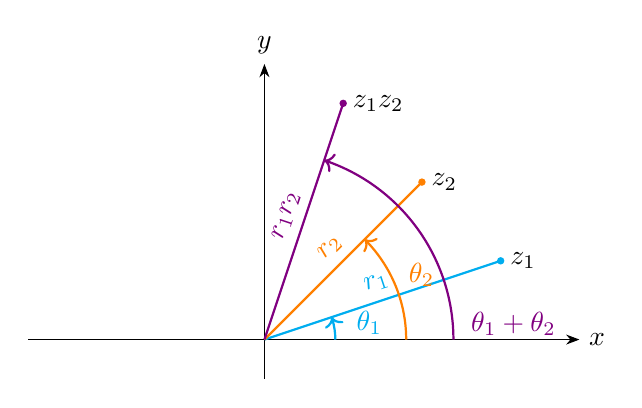
\begin{tikzpicture}[=>stealth]
\draw[-Stealth](-3,0)--(4,0)node[right]{$x$};
\draw[-Stealth](0,-0.5)--(0,3.5)node[above]{$y$};
\draw[thick,cyan](0,0)--node[above,sloped]{$r_1$}(3,1)
(3,1)node[shape=circle,fill=cyan,scale=0.01cm]{};
\draw[thick,orange](0,0)--node[above,sloped]{$r_2$}(2,2)
(2,2)node[shape=circle,fill=orange,scale=0.01cm]{};
\draw[thick,violet](0,0)--node[above,sloped]{$r_1r_2$}(1,3)
(1,3)node[shape=circle,fill=violet,scale=0.01cm]{};
\coordinate (a) at (0.5,0);
\coordinate (b) at (0,0);
\coordinate (c) at (0.5,0.167);
\coordinate (d) at (0.5,0.5);
\coordinate (e) at (0.5,1.5);
\draw
pic[thick,cyan,draw=cyan,angle radius =0.9cm, ->,angle eccentricity=1.5,"$\theta_1$"]{angle = a--b--c};
\draw(3,1)node[right]{$z_1$}
(2,2)node[right]{$z_2$}
(1,3)node[right]{$z_1z_2$}
(2.5,0.2)node[right,violet]{$\theta_1+\theta_2$};
\draw
pic[thick,orange,draw=orange,angle radius = 1.8cm,->,angle eccentricity=1.2,"$\theta_2$"]{angle=a--b--d};
\draw
pic[thick,violet,draw=violet,angle radius=2.4cm,->]{angle=a--b--e};
\end{tikzpicture}
\end{figure}















Also $\hspace{0.3cm} \dfrac{z_1}{z_2} = \dfrac{r_1}{r_2}\big[\cos\big(\theta_1 - \theta_2\big) + i \sin \big(\theta_1 - \theta_2\big)\big]$\\

From this, we can see that \\

$\operatorname{arg}(z_1z_2) = \operatorname{arg}(z_1) + \operatorname{arg}(z_2)$\\

$\Big(\dfrac{z_1}{z_2}\Big) = \operatorname{arg}(z_1) - \operatorname{arg}(z_2)$\\\\



Consider, $\hspace{0.2cm} z = r\big(\cos \theta + i \sin \theta\big)\hspace{0.2cm}$\\

$ z^2 = r^2\big(\cos 2\theta + i \sin 2\theta\big)\hspace{0.2cm}$\\

Using mathematical induction, we can show that $\hspace{0.2cm} z^n = r^n \big( \cos (n\theta) + i \sin (n\theta)\big)$\\

\textbf{\textcolor{teal}{Proof}}
\begin{enumerate}
\item[\textbf{Step 1:}] $n = 1$\\

$z' = r'\big( \cos \theta + i \sin \theta\big)$\\


\item[\textbf{Step 2:}] Suppose $\hspace{0.2cm} z^k = r^k \big( \cos (k\theta) + i \sin (k\theta)\big)$

\begin{align*}
z^{k + 1} & = z^k\cdot z = r^k \big( \cos (k\theta) + i \sin (k\theta)\big)\cdot r \big( \cos (\theta) + i \sin (\theta)\big)\\
& = r^{k + 1}\big( \big(\cos (k\theta)\cos \theta - \sin (k\theta)\sin \theta\big) + i \big( \cos (k\theta)\sin \theta + i\sin (k\theta) \cos \theta)\big)\\
& = r^{k + 1} \big( \cos (k+1)\theta + i \sin (k + 1)\theta\big)
\end{align*}
\end{enumerate}

So by the principal of mathematical induction $\hspace{0.2cm} z^n = r^n \big(\cos (n\theta) + i\sin (n\theta)\big)\hspace{0.1cm},\hspace{0.4cm} \forall\hspace{0.1cm} n \geq 0$\\\\



$\implies\hspace{0.2cm} z^0 = r^0 \big(\cos (0) + i \sin (0)\big) = 1$\\

$\implies\hspace{0.2cm} z^{-1} = \dfrac{1}{z} = \dfrac{1}{r\big(\cos \theta + i\sin \theta\big)}$

\begin{align*}
z^{-1} &  = r^{-1} \hspace{0.1cm} \big( \cos \theta - i \sin \theta\big)\\
& = r^{-1}\hspace{0.1cm} \big(\cos (-\theta) + i \sin (-\theta)\big)
\end{align*}

$$n> 0 \hspace{0.5cm} z^{-n} = r^{-n}\hspace{0.2cm} \big( \cos (-n\theta) + i\sin (-n\theta)\big)$$
 
 
\begin{align*}
z^{-n} & = \big(z^n\big)^{-1} = \dfrac{1}{z^n} = \dfrac{1}{r^n\hspace{0.1cm}\big(\cos(n\theta) + i \sin (n\theta)\big)}\\\\
& = r^{-n}\hspace{0.2cm}\big(\cos (-n\theta) + i\sin (-n\theta)\big)\\
\end{align*} 

$\boxed{ z^n = r^n\hspace{0.2cm} \big( \cos (n\theta) + i\sin (n\theta)\big)\hspace{0.3cm} \forall\hspace{0.1cm}n \in \mathbb{Z}}\hspace{0.4cm}$  De$-$Moivres formula\\\\



\textbf{\textcolor{red}{Example}}\\
Compute $\hspace{0.1cm}z^3\hspace{0.1cm}$ for  $ z = -\sqrt{3} - i$\\

\text{\textcolor{red}{Solution}}\\
In polar form $\hspace{0.2cm} z = 2\Big[ \cos \Big(\dfrac{7\pi}{6}\Big) + i \sin \Big(\dfrac{7\pi}{6}\Big)\Big]$\\

Here $\hspace{0.2cm} r = 2\hspace{0.2cm} , \hspace{0.3cm} \theta = \dfrac{7\pi}{6}\hspace{0.2cm}$ and $\hspace{0.2cm} n = 3$. We get

\begin{align*}
\big(-\sqrt{3} - i\big)^3 & = 2^3 \Big[\cos 3\cdot\dfrac{7\pi}{6} + i \sin 3\cdot \dfrac{7\pi}{6}\Big]\\\\
& = 8 \Big[ \cos \dfrac{7\pi}{2} + i \sin \dfrac{7\pi}{2}\Big]\\\\
& = -8i\\\\
\end{align*}





{\color[wave]{485}\subsection{Powers and Roots}}
Suppose that $\hspace{0.2cm} z = r \big(\cos \theta + i\sin \theta\big)$ and $w = \rho \big( \cos \phi + i \sin \phi\big)$ are polar forms of complex numbers $z$ and $w$.\\

Now consider $\hspace{0.2cm} \rho^n \big(\cos (n\phi) + i\sin(n\phi)\big) = r\big(\cos \theta + i \sin \theta\big)\hspace{0.2cm}$ from this, we have $\hspace{0.2cm} \rho = \sqrt[n]{r}\hspace{0.2cm}$ and $\hspace{0.2cm} \cos n\phi = \cos \theta\hspace{0.2cm}$ and $\hspace{0.2cm} \sin n \phi = \sin \theta$.\\

Hence we have the relationship $\hspace{0.2cm} n \phi = \theta + 2\pi k$ $$\therefore\hspace{0.3cm} \phi = \dfrac{\theta + 2\pi k}{n}\hspace{1cm} k = 0,\hspace{0.2cm} 1,\hspace{0.2cm},\cdots\cdots\cdots , n-1$$

These are distinct roots of $z$. Thus the formula for the $n^{\text{th}}$ roots of a complex number\\ $\hspace{0.2cm} z = r\big( \cos\theta + i \sin \theta\big)$ are given by $$\omega_k = \sqrt[n]{r} \Bigg\{ \cos \Big(\dfrac{\theta + 2\pi k}{n}\Big) + i \sin \Big(\dfrac{\theta + 2\pi k}{n}\Big)\Bigg\}$$\\





\textbf{\textcolor{red}{Example}}\\
Find the cube roots of $\hspace{0.2cm} z = i$\\

\text{\textcolor{red}{Solution}}\\
Here $\hspace{0.2cm} r = 1\hspace{0.2cm},\hspace{0.2cm} \theta = Arg(i) = \dfrac{\pi}{2}\hspace{0.2cm}$ and therefore the polar form of $z$ is $\hspace{0.2cm} z = \cos \dfrac{\pi}{2} + i \sin \dfrac{\pi}{2}$.\\

Hence we obtain
$\omega_k = \displaystyle{\sqrt[3]{1}\Bigg\{ \cos \Big(\dfrac{\dfrac{\pi}{2} + 2\pi k}{3}\Big) + i \sin \Big( \dfrac{\dfrac{\pi}{2} + 2\pi k}{3}\Big)\Bigg\}}\hspace{0.4cm}  k = 0, 1, 2$

\begin{align*}
k = 0\hspace{0.1cm}, \hspace{0.3cm} \omega_0 & = \cos \dfrac{\pi}{6} + i\sin \dfrac{\pi}{6} = \dfrac{\sqrt{3}}{2} + \dfrac{i}{2}\\\\
k = 1\hspace{0.1cm}, \hspace{0.3cm} \omega_1 & = \cos \dfrac{5\pi}{6} + i\sin \dfrac{5\pi}{6} = \dfrac{-\sqrt{3}}{2} + \dfrac{1}{2}i\\\\
k = 2\hspace{0.1cm}, \hspace{0.3cm} \omega_3 & = \cos \dfrac{3\pi}{2} + i\sin \dfrac{3\pi}{2}\\\\
\end{align*}





\textbf{\textcolor{red}{Example}}\\
Find the fourth roots of $\hspace{0.2cm} z = 1 + i$\\  

\text{\textcolor{red}{Solution}}\\
Here $\hspace{0.2cm} r = \sqrt{2}\hspace{0.2cm}$ and $\hspace{0.2cm} \theta = \operatorname{arg}(z) = \dfrac{\pi}{4}\hspace{0.2cm}$ and we get 

$$\omega_k = \sqrt[4]{2}\Bigg\{ \cos \Big(\dfrac{\pi/4 + 2\pi k}{4}\Big) + i \sin \Big(\dfrac{\pi/4 + 2\pi k}{4}\Big)\Bigg\}\hspace{0.5cm} k  = 0, 1, 2,3$$

\begin{align*}
\omega_0 & = \sqrt[4]{2} \Big[ \cos \Big(\dfrac{\pi}{16}\Big) + i\sin \Big(\dfrac{\pi}{16}\Big)\Big]\\\\
\omega_1 & = \sqrt[4]{2} \Big[ \cos \Big(\dfrac{9\pi}{16}\Big) + i\sin \Big(\dfrac{9\pi}{16}\Big)\Big]\\\\
\omega_2 & = \sqrt[4]{2} \Big[ \cos \Big(\dfrac{17\pi}{16}\Big) + i\sin \Big(\dfrac{17\pi}{16}\Big)\Big]\\\\
\omega_3 & = \sqrt[4]{2} \Big[ \cos \Big(\dfrac{25\pi}{16}\Big) + i\sin \Big(\dfrac{25\pi}{16}\Big)\Big]\\\\
\end{align*}









{\color[wave]{485}\subsection{The Exponential Representation}}
We can write any complex number $z = x + iy$ in the form $\displaystyle{z = e^{i\theta}}$ where $\hspace{0.3cm}\displaystyle{e^{i\theta} = \cos \theta + i \sin \theta}$\\

One justification for using this definition is usually the series expansion for exp, cos and sin. We have 
\begin{align*}
e^{i\theta} & = 1 + i\theta + \dfrac{\big(i\theta\big)^2}{2!} + \dfrac{\big(i\theta\big)^3}{3!}+ \cdots\cdots\cdots\\\\
& = 1 + i\theta  - \dfrac{\theta^2}{2!} - \dfrac{i \theta^3}{3!} + \cdots\cdots\cdots\\\\
& = \Bigg(1 - \dfrac{\theta^2}{2!} + \dfrac{\theta^4}{4!} + \cdots\cdots\cdots\Bigg) + i \Bigg( \theta - \dfrac{\theta^3}{3!}+ \cdots\cdots\cdots\Bigg)\\\\
& = \cos \theta + i \sin \theta\\\\
\end{align*}









{\color[wave]{485}\subsection{Lines}}
Suppose we know that the complex point lies on line, and it makes an angle $\theta$ with the real axis, so its slope is $\tan \theta$. Then 
$$\operatorname{arg}(z - a) = \begin{cases}
\theta\\
\pi - \theta\\
\end{cases}$$
defines the locus of points $z$ on the line.\\

Also, $\operatorname{arg}(z - a) = \theta$ represents a half line from a fixed point $a$.\\

Suppose the required line is the perpendicular bisector of the line joining two points $a$ and $b$. Then the locus of $z$ is given by $\hspace{0.2cm} \left|z - a\right| = \left|z - b\right|$\\\\







\textbf{\textcolor{red}{Example}}\\
Trace the locus defined by $\hspace{0.2cm} \operatorname{arg}(z = 3) = \tan^{-1}(2)$\\

\text{\textcolor{red}{Solution}}\\
Let $z = x + iy$, then $\hspace{0.2cm} \operatorname{arg}(x + 3 + iy) = \tan^{-1}(2)$

$$\tan^{-1}\Bigg(\dfrac{y}{x + 3}\Bigg) = \tan^{-1}(2)$$

$$\dfrac{y}{x + 3} = 2$$

$$\implies\hspace{0.3cm} y = 2x + 6$$\\\\





$\mathbb{C}\cup \{\infty\}$\\
Consider $\mathbb{C}$ as contained in $\mathbb{R}^3$ in the form $\hspace{0.1cm} x + iy \longleftrightarrow (x,y) \longleftrightarrow (x,y,0)$ in the $x-y$ plane in $\mathbb{R}^3$.



% DIAGRAM 4

\begin{figure}[H]
\centering
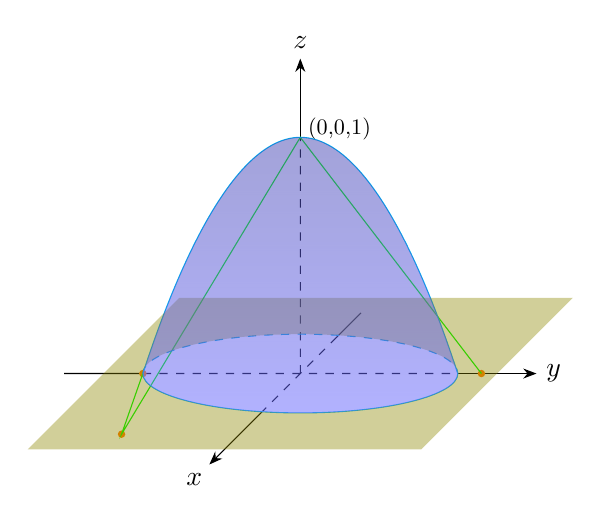
\begin{tikzpicture}[=>stealth]
\draw[-Stealth](2,0)--(3,0)node[right]{$y$};
\draw[-Stealth](0,3,0)--(0,4,0)node[above]{$z$};
\draw[-Stealth](0,0,1.2)--(0,0,3);
\draw[dashed](-2,0,0)--(2,0,0)
(0,0,-1.2)--(0,0,1.2)
(0,0,0)--(0,3,0);
\draw(0,0,3.5)node[]{$x$}
(0,3.1,0)node[right,scale=0.8]{(0,0,1)}
(-3,0,0)--(-2,0,0)
(0,0,-1.2)--(0,0,-2)
(-1.5,0,2)node[shape=circle,fill=orange,scale=0.01cm]{}
(2.3,0,0)node[shape=circle,fill=orange,scale=0.01cm]{}
(-2,0,0)node[shape=circle,fill=orange,scale=0.01cm]{};
\draw[green]
(-2,0,0)--(-1.5,0,2)--(0,3,0)--(2.3,0,0);
\draw[cyan]
(0,3)parabola(2,0)
(0,3)parabola(-2,0)
(-2,0)arc(180:360:2cm and 0.5cm);
\draw[dashed,cyan](-2,0)arc(180:0:2cm and 0.5cm);
\path[fill=olive,opacity=0.4](-2,0)arc(180:360:2cm and 0.5cm)--(2,0)--(2.5,0,0)--(2.5,0,2.5)--(-2.5,0,2.5)--(-2.5,0)--(-2,0)--cycle;
\path[fill=olive,opacity=0.4](-2,0)arc(180:0:2cm and 0.5cm)--(2,0)--(2.5,0,0)--(2.5,0,-2.5)--(-2.5,0,-2.5)--(-2.5,0)--(-2,0)--cycle;
\shade[top color=blue,opacity=0.3](0,3)parabola(-2,0)--(0,0)circle(2cm and 0.5cm)--(2,0)parabola[bend at end](0,3)--cycle;
\shade[bottom color=blue,opacity=0.3](0,3)parabola(-2,0)--(0,0)circle(2cm and 0.5cm)--(2,0)parabola[bend at end](0,3)--cycle;
\end{tikzpicture}
\end{figure}















Consider $\hspace{0.2cm} S = \big\{ (x,y,z):\hspace{0.1cm} x^2 + y^2 +z^2 = 1\big\}$\\

When $z = 0:\hspace{0.2cm} x^2 + y^2 = 1$\\

$\mathcal{Z} = t(0,0,1) + (1-t)(x,y,0)$, $\hspace{0.2cm} t \in \mathbb{R}, \hspace{0.2cm} z \in \mathbb{C}$ is a straight line in $\mathbb{R}^3$ connecting $(0,0,1)$ to $(x,y,z), \hspace{0.2cm} z \in \mathbb{C}$.\\

$\mathcal{Z} = t\big((1-t)x, (1-t)y, t\big)$\\

Putting on a unit sphere, we have
$$\big(1 - t\big)^2 x^2 + \big(1 - t\big)^2 y^2 + t^2 = 1$$
Since $\hspace{0.2cm} \left|z\right|^2 = x^2 + y^2$
$\implies\hspace{0.2cm} \big(1 -t\big)^2\hspace{0.1cm}\left|z\right|^2 + t^2 = 1$\\

$t\neq 1\hspace{0.1cm}$ this corresponds to $(0,0,1)$

\begin{align*}
\implies\hspace{0.5cm} 1 - t^2 & = \big(1- t\big)^2\hspace{0.1cm}\left|z\right|^2\\\\
1 - t^2 & = \left|z\right|^2 + t^2 \left|z\right|^2 - 2t\left|z\right|^2
\end{align*}


$$\implies \hspace{0.3cm} t^2\big(\left|z\right|^2 + 1\big) - 2 t \left|z\right|^2 + \left|z\right|^2 - 1= 0$$



$$ t = \dfrac{\left|z\right|^2 - 1}{\left|z\right|^2 + 1}$$\\



\begin{align*}
\therefore\hspace{0.3cm} \mathcal{Z} & = \Bigg( \dfrac{2x}{\left|z\right|^2 + 1}\hspace{0.2cm},\hspace{0.2cm} \dfrac{2y}{\left|z\right|^2 + 1}\hspace{0.2cm},\hspace{0.2cm}  \dfrac{\left|z\right|^2 - 1}{\left|z\right|^2 + 1}\Bigg)\\\\
& = \Bigg( \dfrac{z + \overline{z}}{\left|z\right|^2 + 1}\hspace{0.2cm},\hspace{0.2cm} \dfrac{-\big(z - \overline{z}\big)}{\left|z\right|^2 + 1}\hspace{0.2cm},\hspace{0.2cm}  \dfrac{\left|z\right|^2 - 1}{\left|z\right|^2 + 1}\Bigg)
\end{align*}

If we are given a point $\mathcal{Z}$ on $S$, then $z$ on $\mathbb{C}$ can be found $\hspace{0.1cm} z = \dfrac{x_1 + ix_2}{1 - x_3}\hspace{0.1cm}$ where $\mathcal{Z} = (x_1, x_2, x_3)$\\

$\mathbb{C}\cup \{\infty\} \longleftrightarrow S\longleftarrow$ Riemann sphere\\

Can give a distance function on $\hspace{0.1cm} \mathbb{C}\cup \{\infty\}$


$$d(z,z') = \begin{cases}
d(\mathcal{Z},\mathcal{Z}')\hspace{0.2cm} (\text{in}\hspace{0.1cm}\mathbb{R}^3)\hspace{0.2cm}\text{where}\hspace{0.2cm}z,z' \neq \infty\\\\
\dfrac{2}{\Big(1 + \left|z\right|^2\Big)^{1/2}}\hspace{0.4cm}\text{if}\hspace{0.4cm}z' = \infty\\
\end{cases}
$$


$$d(z,z') = \begin{cases}
\Big[\big(x_1 -x_1'\big)^2 + \big(x_2 - x'_2\big)^2 + \big(x_3 - x'_3\big)\Big]^{1/2}\\\\
\dfrac{2}{\Big(1 + \left|z\right|^2\Big)^{1/2}}\hspace{0.4cm}\text{if}\hspace{0.4cm}z' = \infty\\
\end{cases}
$$















This correspondence is called sterographic projection\\

\begin{align*}
\mathbb{C}\cup \{\infty\}\hspace{2cm} a + \infty & = \infty\hspace{0.5cm} a\in \mathbb{C}\\
a\cdot \infty & = \infty \hspace{0.5cm} a\in \mathbb{C}\hspace{0.2cm},\hspace{0.5cm} a\neq 0\\
\dfrac{a}{\infty} & = 0\hspace{0.5cm} a\in \mathbb{C}
\end{align*}
















\pagebreak
{\color[wave]{485}\section{Elementary Theory of Power series}}

{\color[wave]{485}\subsection{Sequences}}

\textbf{\textcolor{teal}{Definition}}\\
A sequence $\{z_n\}$ is a function where the domain is the set of positive integers and whose range is a subset of the complex numbers.\\



If $\lim\limits_{n \rightarrow \infty} z_n = L$, we say the sequence $\{z_n\}$ is convergent. The number $L$ is called the limit of $(z_n)$\\\\



\textbf{\textcolor{teal}{Definition}}\\
A sequence $\{z_n\}$ converges to the number $L$ if $\forall\hspace{0.1cm} \varepsilon > 0$ and $N$ exist such that $\hspace{0.2cm}\left|z_n - L\right| < \varepsilon\hspace{0.2cm}$ whenever $n<N$.\\



A sequence that is not convergent is said to be divergent.\\\\



\textbf{\textcolor{red}{Example}}\\
The sequence $\hspace{0.2cm}\displaystyle{\Big\{\dfrac{i^{n + 1}}{n}\Big\}}\hspace{0.2cm}$ converges, since $\hspace{0.2cm} \lim\limits_{n\rightarrow \infty} \dfrac{i^{1 + n}}{n} = 0$.\\

As we see from this $\hspace{0.2cm}\displaystyle{-1,\hspace{0.2cm} \dfrac{-i}{2}, \hspace{0.2cm} \dfrac{1}{3},\hspace{0.2cm}\dfrac{i}{1}, \hspace{0.2cm}, \dfrac{-1}{5}}$.\\\\



\textbf{\textcolor{teal}{Theorem}}\\
A sequence $\{z_n\}$ converges to a complex number $L = a + ib$ if and only if $\operatorname{Re}(z_n)$ converges to $\operatorname{Re}(L)= a$ and $\operatorname{Im}(z_n)$ converges to $\operatorname{Im}(L) = b$.\\


\textbf{\textcolor{teal}{Proof}}\\
Assume that $z_n \longrightarrow L$. Then $\forall \hspace{0.1cm} \varepsilon > 0\hspace{0.1cm} \exists\hspace{0.1cm} N_{\varepsilon} \ni \left|z_n - L\right| < \varepsilon\hspace{0.2cm} \forall\hspace{0.1cm} n> N_{\varepsilon}$. But $$\left|\operatorname{Re}(z_n - L)\right| \leq \left|z_n - L\right|< \varepsilon$$
That is, $\operatorname{Re}(z_n) \longrightarrow \operatorname{Re}(L)$. Similarly, one can show that $\operatorname{Im}(z_n) \longrightarrow \operatorname{Im} (L)$.\\

Conversely, assume that (abbreviating $x = \operatorname{Re} (L)$ and $y = \operatorname{Im} (L))$\\ $\hspace{0.2cm} \forall\hspace{0.1cm} \varepsilon > 0\hspace{0.1cm}  \exists\hspace{0.1cm} N_{\varepsilon} \ni \left|x_n - x\right|,\hspace{0.1cm}\left|y_n - y\right| < \dfrac{\varepsilon}{2}\hspace{0.2cm}\forall\hspace{0.1cm}n>N_{\varepsilon}$. Then by the triangle inequality $$ \left|z_n - L\right| \leq \left|x_n - x\right| + \left|y_n - y\right| < \dfrac{\varepsilon}{2} + \dfrac{\varepsilon}{2} = \varepsilon$$
$\implies\hspace{0.2cm}  z_n \longrightarrow L$ as $n \longrightarrow \infty.$\\\\\\




\textbf{\textcolor{red}{Example}}\\
Consider the sequence $\displaystyle{\Big\{\dfrac{3 + ni}{n + 2ni}\Big\}}$\\



\pagebreak
\text{\textcolor{red}{Solution}}
\begin{align*}
\text{From}\hspace{1cm} z_n & = \dfrac{3 + ni}{n + 2ni} = \dfrac{(3 + ni) (n-2ni)}{n^2 + 4n^2}\\\\
& = \dfrac{2n^2 + 3n}{5n^2} + i\hspace{0.1cm}\dfrac{n^2 - 6n}{5n^2}
\end{align*}
we see that\\

$\operatorname{Re}(z_n) = \dfrac{2n^2 + 3n}{5n^2} = \dfrac{2}{5} + \dfrac{3}{5n} \longrightarrow \dfrac{2}{5}$ as $n\longrightarrow \infty$\\

$\operatorname{Im}(z_n) = \dfrac{n^2 - 6n}{5n^2} = \dfrac{1}{5} - \dfrac{6}{5n}\longrightarrow \dfrac{1}{5}$ as $n \longrightarrow \infty$\\

Hence $\hspace{0.2cm} z_n \longrightarrow \dfrac{2}{5} + i\hspace{0.1cm}\dfrac{1}{5}$\\\\\\



\textbf{\textcolor{teal}{Definition}}\\
A sequence $\{z_n\}_{n\geq 1}$ is said to be Cauchy if $\forall \hspace{0.1cm} \varepsilon > 0, \exists\hspace{0.1cm} n_0 \in \mathbb{N} \ni n,m \geq n_0,\hspace{0.1cm}\left|z_m - z_n\right| < \varepsilon$.\\\\



\textbf{\textcolor{teal}{Proposition}}\\
A complex sequence is convergent if and only if it is a Cauchy sequence.\\\\\\






{\color[wave]{485}\subsection{Complex Series}}
Let $(z_n)$ be a sequence of complex numbers. The form sum $\hspace{0.2cm} a_1 + a_2+ \cdots\cdots\cdots\hspace{0.2cm}$ is called the series $\hspace{0.2cm}\displaystyle{ \sum a_n}$.\\

$\implies\hspace{0.2cm}$ The series $\displaystyle{\sum a_n}$ is said to converge to the sum(s) if the sequence of partial sums $(S_n)$ given by $$ S_n = a_1 + a_2 + \cdots\cdots\cdots + a_n = \sum^n_{j=1}a_j$$ Converges to the limit $(S)$ $\hspace{0.3cm} S = \displaystyle{\sum^{\infty}_{j=1}a_j}$\\

$\implies\hspace{0.2cm}$ If the sequence $(S_n)$ does not converge, then we say that the series $\displaystyle{\sum a_n}$ does not converge.\\\\




\textbf{\textcolor{teal}{Proposition}}\\
$\displaystyle{\sum z_n}$ converges if and only if $\displaystyle{\sum \operatorname{Re}(z_n)}$ and $\displaystyle{\sum \operatorname{Im} (z_n)}$ both converges.\\\\



\pagebreak
\textbf{\textcolor{teal}{Properties}}
\begin{enumerate}
\item
\begin{enumerate}
      \item If $\displaystyle{\sum z_n}$ converges then $\hspace{0.1cm} \lim\limits_{n\rightarrow \infty} z_n = 0$
      
      \item there is a $\hspace{0.1cm} M\in \mathbb{R},\hspace{0.1cm}\exists \hspace{0.1cm} M\geq 0 \in \mathbb{R} \ni \left|z_n\right|\leq, \hspace{0.2cm} \forall\hspace{0.1cm} n \in \mathbb{N}$
\end{enumerate}

\item If $\displaystyle{\sum a_n}$ and $\displaystyle{\sum b_n}$ are both convergent complex series then $\displaystyle{\sum \big(a_n + C b_n\big)}$ is also convergent complex series $\forall\hspace{0.1cm}C \in \mathbb{R}$.


\item \textit{Absolute Convergent}\\
A series $\displaystyle{\sum z_n}$ is said to be absolutely convergent if the series $\displaystyle{\sum\left|z_n\right|}$ converges.\\
$\implies$ Suppose that the real series $\displaystyle{\sum \left|z_n\right|}$ converges then $\displaystyle{\sum z_n}$ converges.


\item \textit{Test for Convergence}\\
We can apply comparison, ratio test and Cauchy's $n^{\text{th}}$ ratio test to test the convergence of $\displaystyle{\sum z_n}$ and $\displaystyle{\sum \left|z_n\right|}$ is convergent then $\displaystyle{\sum z_n}$ is convergent by property (3)\\\\\\
\end{enumerate}





{\color[wave]{485}\subsection{Uniform Convergence}}

The notes go on to differentiate and integrate series term by term. That step is
not free, and uniform convergence is the hypothesis that pays for it. The
distinction below is the whole of the matter.

\textbf{\textcolor{teal}{Definition: pointwise and uniform convergence}}\\
Let $f_n$ and $f$ be functions on a set $S \subseteq \mathbb{C}$.
\begin{enumerate}
\item[(i).] $f_n \rightarrow f$ \emph{pointwise} on $S$ if for every $z \in S$
and every $\varepsilon > 0$ there is $N$, possibly depending on both $z$ and
$\varepsilon$, with $\left|f_n(z) - f(z)\right| < \varepsilon$ for all $n \geq N$.
\item[(ii).] $f_n \rightarrow f$ \emph{uniformly} on $S$ if for every
$\varepsilon > 0$ there is $N$, depending on $\varepsilon$ \emph{alone}, with
$$\left|f_n(z) - f(z)\right| < \varepsilon \hspace{0.4cm}\text{for all } n \geq N
\hspace{0.2cm}\text{and all } z \in S .$$
\end{enumerate}

The single word that separates them is \emph{alone}. Under pointwise convergence
each point may demand its own $N$, and there need be no bound on how large those
$N$ have to be as $z$ moves about $S$; under uniform convergence one $N$ serves
the whole set at once.

\textbf{\textcolor{red}{Example}}\\
On $S = \{\left|z\right| < 1\}$ take $f_n(z) = z^n$. Then $f_n \rightarrow 0$
pointwise, since $\left|z\right| < 1$ gives $\left|z\right|^n \rightarrow 0$. The
convergence is \emph{not} uniform on $S$: taking $z$ with
$\left|z\right| = 1 - \tfrac{1}{n}$ gives
$\left|f_n(z)\right| = \left(1 - \tfrac{1}{n}\right)^n \rightarrow e^{-1}$,
which does not go to $0$, so no single $N$ can work everywhere. On the smaller
disc $\left|z\right| \leq r$ with $r < 1$ the convergence \emph{is} uniform,
because $\left|f_n(z)\right| \leq r^n \rightarrow 0$ with a bound independent of
$z$.

That example is the pattern for power series generally: uniform on every closed
disc strictly inside the circle of convergence, and typically not on the open
disc itself.

\textbf{\textcolor{teal}{Theorem: the Weierstrass $M$-test}}\\
Let $\displaystyle\sum^{\infty}_{n = 1} u_n(z)$ be a series of functions on
$S$, and suppose there are constants $M_n$ with
$$\left|u_n(z)\right| \leq M_n \hspace{0.4cm}\text{for all } z \in S,
\hspace{0.6cm}\text{and}\hspace{0.6cm}
\sum^{\infty}_{n=1} M_n < \infty .$$
Then $\displaystyle\sum u_n$ converges absolutely and uniformly on $S$.

\textbf{\textcolor{teal}{Proof}}\\
Absolute convergence at each point is immediate by comparison with
$\sum M_n$. Write $s(z)$ for the sum and $s_N(z)$ for the $N$-th partial sum.
Then for every $z \in S$
$$\left|s(z) - s_N(z)\right| = \left|\sum^{\infty}_{n = N+1} u_n(z)\right|
\leq \sum^{\infty}_{n = N+1}\left|u_n(z)\right|
\leq \sum^{\infty}_{n = N+1} M_n .$$
The right-hand side is the tail of a convergent series of constants, so it can be
made smaller than any $\varepsilon > 0$ by choosing $N$ large --- and that choice
does not involve $z$. $\blacksquare$

The $M$-test is the workhorse: it converts a question about functions into a
question about a series of numbers.

\textbf{\textcolor{teal}{Theorem}}\\
A uniform limit of continuous functions is continuous. That is, if each $f_n$ is
continuous on $S$ and $f_n \rightarrow f$ uniformly on $S$, then $f$ is
continuous on $S$.

\textbf{\textcolor{teal}{Proof}}\\
Fix $z_0 \in S$ and $\varepsilon > 0$. Choose $N$ with
$\left|f_N(z) - f(z)\right| < \tfrac{\varepsilon}{3}$ for all $z \in S$, which
uniformity permits. Since $f_N$ is continuous at $z_0$ there is $\delta > 0$ such
that $\left|z - z_0\right| < \delta$ gives
$\left|f_N(z) - f_N(z_0)\right| < \tfrac{\varepsilon}{3}$. Then for such $z$
$$\left|f(z) - f(z_0)\right| \leq \left|f(z) - f_N(z)\right| +
\left|f_N(z) - f_N(z_0)\right| + \left|f_N(z_0) - f(z_0)\right|
< \tfrac{\varepsilon}{3} + \tfrac{\varepsilon}{3} + \tfrac{\varepsilon}{3}
= \varepsilon . \hspace{0.3cm}\blacksquare$$

The three-way split above is worth remembering; it recurs whenever a uniform
estimate is traded for a local one.

\textbf{\textcolor{teal}{Theorem: term-by-term integration}}\\
If $f_n \rightarrow f$ uniformly on a contour $C$ of finite length $L$, and each
$f_n$ is continuous on $C$, then
$$\lim_{n \rightarrow \infty}\int_C f_n(z)\,dz = \int_C f(z)\,dz .$$

\textbf{\textcolor{teal}{Proof}}\\
Given $\varepsilon > 0$ pick $N$ so that
$\left|f_n(z) - f(z)\right| < \dfrac{\varepsilon}{L}$ on $C$ for $n \geq N$. By
the estimation (ML) inequality,
$$\left|\int_C f_n(z)\,dz - \int_C f(z)\,dz\right|
= \left|\int_C \big(f_n(z) - f(z)\big)dz\right|
\leq \dfrac{\varepsilon}{L}\cdot L = \varepsilon . \hspace{0.3cm}\blacksquare$$

Note where uniformity was used: the bound $\varepsilon / L$ had to hold at every
point of $C$ at once. Pointwise convergence gives no such bound and the theorem
is false without it.

\textbf{\textcolor{teal}{Theorem: Weierstrass' theorem on analytic limits}}\\
Let $f_n$ be analytic on a domain $D$ and suppose $f_n \rightarrow f$ uniformly
on every compact subset of $D$. Then $f$ is analytic on $D$, and moreover
$f_n' \rightarrow f'$ uniformly on every compact subset of $D$.

\textbf{\textcolor{teal}{Proof (outline)}}\\
$f$ is continuous by the theorem above. For any triangle $\Delta$ with its
interior contained in $D$, Cauchy's theorem gives
$\int_{\partial \Delta} f_n = 0$, and term-by-term integration passes to the
limit to give $\int_{\partial \Delta} f = 0$. Morera's theorem then makes $f$
analytic. The statement about derivatives follows from the Cauchy integral
formula for $f'$ applied to $f_n - f$ on a circle inside $D$. $\blacksquare$

This is the result that licenses differentiating a power series term by term, and
it has no analogue for real functions: a uniform limit of real polynomials need
not be differentiable even once, whereas here the limit is infinitely
differentiable.

\textbf{\textcolor{teal}{Corollary: power series converge uniformly on compact subdiscs}}\\
If $\displaystyle\sum a_n (z - z_0)^n$ has radius of convergence $R > 0$, then
for every $r$ with $0 < r < R$ the series converges uniformly on
$\left|z - z_0\right| \leq r$.

\textbf{\textcolor{teal}{Proof}}\\
Pick $\rho$ with $r < \rho < R$. Since $\rho < R$ the series
$\sum \left|a_n\right| \rho^n$ converges. On $\left|z - z_0\right| \leq r$,
$$\left|a_n (z - z_0)^n\right| \leq \left|a_n\right| r^n
= \left|a_n\right|\rho^n \left(\dfrac{r}{\rho}\right)^n
\leq \left|a_n\right| \rho^n =: M_n ,$$
and $\sum M_n < \infty$. The Weierstrass $M$-test applies. $\blacksquare$

Consequently a power series is analytic inside its circle of convergence and may
be differentiated and integrated term by term there --- which is what the rest of
this course assumes throughout.



{\color[wave]{485}\subsection{Power Series}}
\textit{A Power Series}: A series of the form $\hspace{0.2cm}a_0 + a_1z + a_2z^2 + \cdots\cdots\cdots\hspace{0.2cm}$ where $a_i\in \mathbb{C}$ is called a power series around 0 in the variable $z$.\\




\textbf{\textcolor{blue}{Note}}
\begin{enumerate}
\item[$\implies$] Power series around $0$ converges for $z = 0$
\item[$\implies$] Power series around $a$ converges for $z = a$\\
\end{enumerate}



A power series is said to be convergent at a point $z  = z_0$ if the partial sums $S_n$ evaluated at $z_0$ converges to a limit.\\\\





\textbf{\textcolor{red}{Example}}: Geometric series\\

$\displaystyle{1 + z + z^2 + \cdots\cdots\cdots\cdots}$\\

$\displaystyle{(1 - z)\big(1 + z + z^2 + \cdots\cdots\cdots + z^n\big) = 1 - z^{n+1}}$\\

$\displaystyle{1 + z + z^2 + \cdots\cdots\cdots + z^n = \dfrac{1 - z^{n + 1}}{1 - z}}\hspace{0.2cm}$ if $z\neq 1$\\

Since $\lim\limits_{n\rightarrow \infty} z^{n + 1} = 0$ if $ \left|z\right| < 1$.\\

when $\left|z\right| < 1$ the geometric series $\displaystyle{\sum^{\infty}_{n = 0}z^n}$ converges to $\dfrac{1}{1 - z}$\\

$z^{n + 1}$ diverges for $\left|z\right|> 1$.\\

So, $\displaystyle{\sum z^n = \begin{cases}
\text{converges}\hspace{0.2cm} \dfrac{1}{1 - z}\hspace{0.2cm}\text{when}\hspace{0.2cm} \left|z\right| < 1\\\\
\text{diverges when}\hspace{0.2cm}\left|z\right|> 1\\
\end{cases}
}$\\\\



\textbf{\textcolor{teal}{Theorem}}\\
To each power series $\displaystyle{\sum a_n z^n}$ there exists a corresponding $R$ with $0\leq R\leq \infty$ called the radius of convergence, with the following properties
\begin{enumerate}
\item[i).] $\displaystyle{\sum a_n z^n}$ converges absolutely for every $z$ with $\left|z\right| < R$.
\item[ii).] If $\left|z\right|> R$, the terms of the series are unbounded and hence the series is divergent.\\
\end{enumerate}

\textbf{\textcolor{teal}{Proof}}
\begin{enumerate}
\item[i).] Let $R = \sup \big\{\left|z\right|:\hspace{0.2cm} \sum \left|a_n z^n\right|\hspace{0.2cm} \text{converges}\big\}$. If $\left|z\right| < R$ then there is a $z_1\ni \left|z\right| < \left|z_1\right| < R$ and $\displaystyle{\left|a_nz_1^n\right|}$ converges.\\
Now there is an $\hspace{0.2cm}M\geq 0 \ni \left|a_nz_1^n\right|\leq M \hspace{0.2cm} \forall n \geq 0\hspace{0.2cm} \cdots\cdots\cdots\hspace{0.2cm}(*) \hspace{0.3cm}$ then 
\begin{align*}
\left|a_nz^n\right| & = \left|a_n\right|\hspace{0.1cm}\left|\dfrac{z}{z_1}\right|^n\hspace{0.1cm}\left|z_1\right|^n\\\\
& \leq M\hspace{0.1cm}\left|\dfrac{z}{z_1}\right|^n\hspace{0.3cm} \text{by}\hspace{0.2cm}(*)
\end{align*}

Since $\hspace{0.1cm}\displaystyle{\left|\dfrac{z}{z_1}\right| < 1}$\\

$\displaystyle{\sum M \left|\dfrac{z}{z_1}\right|^n = M \sum \left|\dfrac{z}{z_1}\right|^n}\hspace{0.2cm}$ converges and so by comparison test $\displaystyle{\sum a_n z^n}$ converges absolutely.\\\\


\item[ii).] If $\left|z\right|>R$ and if $\displaystyle{a_nz^n}$ is convergent then there is an $M\geq 0 \ni \left|a_n z^n\right| \leq M,\hspace{0.2cm} \forall\hspace{0.1cm} n\geq 0$.\\
So, $\forall\hspace{0.1cm} w \in \mathbb{C}$ with $\left|z\right| > \left|w\right| >R$
$$\left|a_nw^n\right| \leq \left|a_nz^n\right|\hspace{0.1cm}\left|\dfrac{w}{z}\right|^n \leq M\hspace{0.1cm}\left|\dfrac{w}{z}\right|^n$$
Since $\displaystyle{\sum M\hspace{0.1cm}\left|\dfrac{w}{z}\right|^n}$ is a convergent geometric series. $\displaystyle{\sum \left|a_nw^n\right|}$ is also convergent by comparison test.\\
This is a contradiction to the definition of $R$. So $\displaystyle{\sum a_n z^n}$ is divergent for $\left|z\right|> R$.\\\\
\end{enumerate}




$\star$ Determination of the radius of convergence of a given power series can be done using the ratio or the root test.\\\\




\textbf{\textcolor{red}{Example}}\\
Consider the series $\hspace{0.2cm}\displaystyle{\sum^{\infty}_{n = 0} \dfrac{z^n}{n!}}$\\

$\therefore$ By ratio test, this series converges absolutely when
\begin{align*}
\lim\limits_{n\rightarrow \infty} \left|\dfrac{z^{n+1}\big/\big(n+1\big)!}{z^n\big/n!}\right|& < 1\\\\
\lim\limits_{n \rightarrow\infty} \left|\dfrac{z}{n+1}\right| & < 1
\end{align*}
$0 < 1 \hspace{0.1cm}$ is always true independent for any $z\in \mathbb{C}$, this converges absolutely.
i.e the radius of convergence is $\infty$.\\\\





$\star$ Cauchy$-$Hadamad formula for radius of convergence.\\
$\therefore$ The series $\displaystyle{\sum a_n z^n}$ has radius of convergence $R$ where $R$ is given by 
$$\dfrac{1}{R} = \lim \sup \Big\{\sqrt[n]{\left|a_n\right|}\Big\}$$


$$\dfrac{1}{0} = \infty \hspace{0.2cm}, \hspace{0.2cm} \dfrac{1}{\infty}= 0$$


\textbf{\textcolor{blue}{Note:}} this limit always exists it could equal $\infty$.\\\\



\textbf{\textcolor{red}{Example}}\\
Determine the radius of convergence $R$ of the power series $\hspace{0.2cm} \displaystyle{\sum^{\infty}_{n = 0} \dfrac{\big(2n\big)!}{\big(n!\big)^2}\hspace{0.1cm}\big(z - 3i\big)^n}$

\begin{align*}
L^* & = \lim\limits_{n\rightarrow \infty} \left|\dfrac{\big(2n + 2\big)!}{\big((n+1)!\big)^2}\div \dfrac{\big(2n)!}{\big(n!\big)^2}\right|\\\\
& = \lim\limits_{n\rightarrow \infty} \dfrac{\big(2n + 2\big)\big(2n+1\big)}{\big(n + 1\big)^2}\\\\
& = 4
\end{align*}
Hence $R = \dfrac{1}{L^*} = \dfrac{1}{4}$. The series converges in the disk $\left|z - 3i\right|< \dfrac{1}{4}$ of radius $\dfrac{1}{4}$ and center $3i$.\\























\pagebreak
{\color[wave]{485}\section{Elementary Point Set Topology of $\mathbb{C}$}}

\textbf{\textcolor{teal}{Definition}}\\
A metric space is a pair $(X,d)$ where $X$ is a set and $d$ is a function from $X\times X$ into $\mathbb{R}$, called a distance function or metric, which satisfies the following conditions for $x,y,  z \in X$.
\begin{enumerate}
\item $d(x,y) \geq 0$

\item $d(x,y)  = 0\hspace{0.2cm}$ if and only if $\hspace{0.2cm} x = y$

\item $d(x,y) = d(y,x)\hspace{0.2cm}$ (symmetry)

\item $d(x,z) \leq d(x,y) + d(y,z)\hspace{0.2cm}$ (triangle inequality)\\\\
\end{enumerate}





$*\hspace{0.2cm} B(a;r) = \big\{z \in \mathbb{C}:\hspace{0.2cm} \left|z - a\right| < r\big\}\hspace{0.2cm}$ (open ball of radius $r$, centred at $a$)\\



$\left|z\right|:\hspace{0.2cm}$ distance between 0 and $z$ in the complex plane.

% DIAGRAM 1


\begin{figure}[H]
\centering
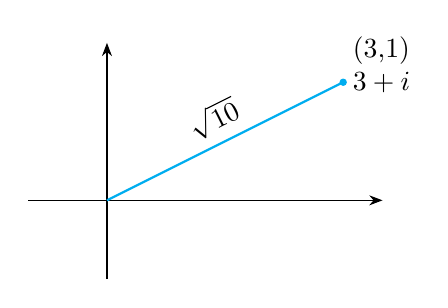
\begin{tikzpicture}[=>stealth]
\draw[-Stealth](-1,0)--(3.5,0);
\draw[-Stealth](0,-1)--(0,2);
\draw[thick,cyan](0,0)--node[sloped,black,above]{$\sqrt{10}$}(3,1.5);
\draw(3,1.5)node[shape=circle,fill=cyan,scale=0.01cm]{}
(3,1.9)node[right]{(3,1)}
(3,1.5)node[right]{$3+i$};
\end{tikzpicture}
\end{figure}













$\implies \hspace{0.2cm} \left|z_1 - z_0\right|:\hspace{0.2cm}$ distance between complex numbers $z_1$ and $z_0$ in the complex number.

% DIAGRAM 2

\begin{figure}[H]
\centering
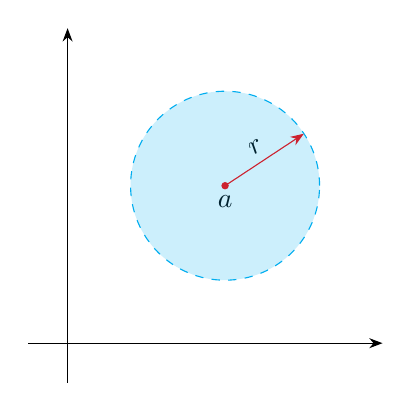
\begin{tikzpicture}[=>stealth]
\draw[-Stealth](-2.5,-2)--(2,-2);
\draw[-Stealth](-2,-2.5)--(-2,2);
\draw[dashed,cyan](0,0)circle[radius=1.2cm];
\draw(0,0)node[shape=circle,fill=red,scale=0.01cm]{}
(0,0)node[below]{$a$};
\draw[red,red,-Stealth](0,0)--node[above,sloped,black]{$r$}(1,0.66);
\path[fill=cyan,opacity=0.2](0,0)circle[radius=1.2cm];
\end{tikzpicture}
\end{figure}
















\textbf{\textcolor{red}{Example}}\\

$B(i;1) = \{z \in \mathbb{C}:\hspace{0.2cm}\left|z - i\right| < 1\}$


% DIAGRAM 3


\begin{figure}[H]
\centering
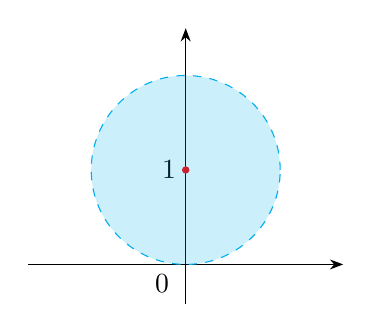
\begin{tikzpicture}[=>stealth]
\draw[-Stealth](-2,0)--(2,0);
\draw[-Stealth](0,-0.5)--(0,3);
\draw[dashed,cyan](0,1.2)circle[radius=1.2cm];
\draw(0,1.2)node[shape=circle,fill=red,scale=0.01cm]{}
(0,1.2)node[left]{$1$}
(-0.3,0)node[below]{0};
\path[fill=cyan,opacity=0.2](0,1.2)circle[radius=1.2cm];
\end{tikzpicture}
\end{figure}
















$*\hspace{0.2cm} \overline{B(a; r)} = \big\{ z \in \mathbb{C}: \hspace{0.2cm} \left|z - a\right| \leq r\big\}\hspace{0.2cm}$ ( closed ball of radius $r$ centred at $a$)\\\\

$*\hspace{0.2cm} \overline{B(a ; r)} - B(a ; r) = \big\{z\in \mathbb{C}:\hspace{0.2cm} \left|z - a\right| = r \big\}\hspace{0.2cm}$ ( sphere)\\\\




$\implies\hspace{0.3cm}$ upper half plane is the set
$$\boxed{\pi = \big\{z \in \mathbb{C}:\hspace{0.2cm} \operatorname{Im} (z) > 0\big\}}$$


% DIAGRAM 4

\begin{figure}[H]
\centering
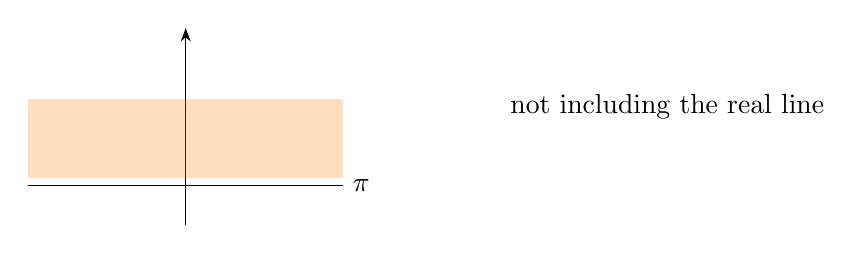
\begin{tikzpicture}[=>stealth]
\draw(-2,0)--(2,0)node[right]{$\pi$};
\draw[-Stealth](0,-0.5)--(0,2);
\draw(4,1)node[right]{not including the real line};
% A solid wash rather than TikZ's `pattern=` hatching. tex4ht converts each
% picture by way of PostScript, and pgf's pattern definitions are undefined
% there - the conversion fails with "PostScript error: undefined in pgfpat1"
% and simply writes no file, so the page ends up with a broken image and
% nothing in the log to say a figure is missing. The hatch only marked which
% region was meant; a wash of the same colour says the same thing.
\path[fill=orange,opacity=0.25](-2,0.1)--(2,0.1)--(2,1.1)--(-2,1.1)--cycle;
\end{tikzpicture}
\end{figure}









\vspace{0.5cm}






$\implies\hspace{0.3cm} $ Annulus: A set of the kind
$$\boxed{\big\{ z \in \mathbb{C}:\hspace{0.2cm} r_1 < \left|z - a\right| < r_2\big\}}$$

% DIAGRAM 5


\begin{figure}[H]
\centering
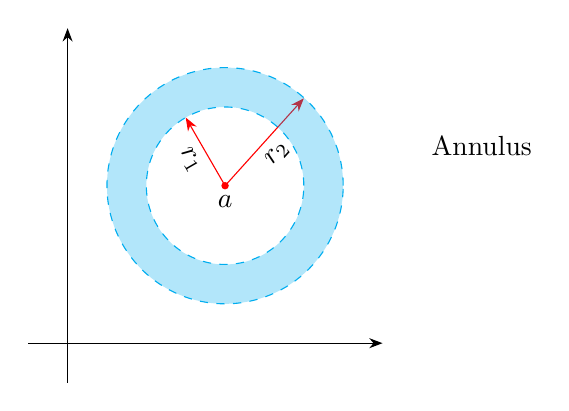
\begin{tikzpicture}[=>stealth]
\draw[cyan,dashed](0,0)circle[radius=1cm]
(0,0)circle[radius=1.5cm];
\draw(0,0)node[shape=circle,fill=red,scale=0.01cm]{}
(0,0)node[below]{$a$}
(2.5,0.5)node[right]{Annulus};
\draw[-Stealth,red](0,0)--node[below,sloped,black]{$r_1$}(-0.5,0.866);
\draw[-Stealth,red](0,0)--node[below,sloped,black]{$r_2$}(1,1.11);
\path[fill=cyan,opacity=0.3](-1,0)arc[start angle = 180,end angle = 360, radius=1cm]--(1,0)--(1.5,0)--(1.5,0)arc[start angle =0,end angle = -180, radius=1.5cm]--(-1.5,0)--(-1,0)--cycle
(1,0)arc[start angle = 0,end angle = 180, radius = 1cm]--(-1,0)--(-1.5,0)--(-1.5,0)arc[start angle = 180, end angle = 0,radius=1.5cm]--(1.5,0)--(1,0)--cycle;
\draw[-Stealth](-2.5,-2)--(2,-2);
\draw[-Stealth](-2,-2.5)--(-2,2);
\end{tikzpicture}
\end{figure}


















\vspace{1cm}
\textbf{\textcolor{teal}{Definition}}\\
The deleted neighbourhood of point $a\in \mathbb{C}$ is the set $$ \big\{z \in \mathbb{C}:\hspace{0.2cm} 0 < \left|z - a\right| < r\big\}$$ for some positive real number $r$. This is denoted by $B'(a ; r)$.

% DIAGRAM 6


\begin{figure}[H]
\centering
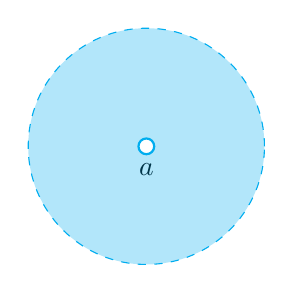
\begin{tikzpicture}[=>stealth]
\draw[cyan,thick](0,0)circle[radius=0.1cm];
\draw[dashed,cyan](0,0)circle[radius=1.5cm];
\draw
(0,-0.1)node[below]{$a$};
\path[fill=cyan,opacity=0.3](-0.1,0)arc[start angle = 180,end angle = 360, radius=0.1cm]--(0.1,0)--(1.5,0)--(1.5,0)arc[start angle =0,end angle = -180, radius=1.5cm]--(-1.5,0)--(-0.1,0)--cycle
(0.1,0)arc[start angle = 0,end angle = 180, radius = 0.1cm]--(-0.1,0)--(-1.5,0)--(-1.5,0)arc[start angle = 180, end angle = 0,radius=1.5cm]--(1.5,0)--(0.1,0)--cycle;
\end{tikzpicture}
\end{figure}















\textbf{\textcolor{teal}{Definition}}\\
A set $\hspace{0.2cm} A \subseteq \mathbb{C}\hspace{0.2cm}$ is open if for every $z \in A$, there exist $r>0,\hspace{0.2cm} r(z)\hspace{0.2cm}$ such that $\hspace{0.2cm} B(z ; r )\subseteq A$.\\\\




\textbf{\textcolor{red}{Example}}\\
$B(a ; r)\hspace{0.2cm}$ is  an open set.\\


\textcolor{teal}{Proof}\\
Let $\hspace{0.2cm} z \in B(a; r) = \big\{ z \in \mathbb{C}:\hspace{0.2cm} \left|z -a\right| < r\big\}$\\

$\left|z - a\right| < r\hspace{0.2cm}$ so $\hspace{0.2cm} 0 < r - \left|z - a\right|$\\

Let $\hspace{0.2cm} \delta\hspace{0.2cm}$ be $\ni\hspace{0.2cm} 0 < \delta < r - \left|z - a\right|$\\











Then if $\hspace{0.2cm} w \in B(z; \delta)$
\begin{align*}
\left|w - z\right| < \delta \hspace{0.2cm} \implies \hspace{0.2cm} \left|w - a\right| & \leq \left|w - z\right| + \left|z - a\right|\\
& \leq  \delta + \left|z - a\right|\\
&< r
\end{align*}

Since $\hspace{0.2cm} (0 < \delta < r - \left|z - a\right|)\hspace{0.2cm}$ we have that $\hspace{0.2cm}\left|w - a\right| < r\hspace{0.2cm}$ so $\hspace{0.2cm} w \in B(a;r)$\\

$\implies \hspace{0.2cm} B(z; \delta) \subseteq B(a; r)$\\

Since $z$ was arbitrary point of $B(a;r),\hspace{0.2cm} B(a;r)\hspace{0.2cm}$ is an open set.\\\\\\





{\color[wave]{485}\subsection{Generating Open Sets}}
\begin{enumerate}
\item The empty set is open
\item The entire complex plane is an open set.
\item If $\hspace{0.2cm} S_1, \hspace{0.1cm} S_2\hspace{0.2cm}$ are open sets then $S_1 \cap S_2$ is open.
\item If $\big\{S_{\alpha}\big\}_{\alpha \in A}\hspace{0.2cm}$ ($A$ is some index set) is an arbitrary collection open sets in $\mathbb{C}$ then $\hspace{0.2cm} \bigcup\limits_{\alpha \in A}S_{\alpha}\hspace{0.2cm}$ is an open set.\\\\ 
\end{enumerate}








\textbf{\textcolor{red}{Example}}
\begin{enumerate}
\item $\hspace{0.2cm} \big\{z \in \mathbb{C}:\hspace{0.2cm} \left|z - a\right| > r\big\}\hspace{0.2cm}$ is an open set.

\item $\hspace{0.2cm} \big\{z \in \mathbb{C}:\hspace{0.2cm} \left|z - a\right| > r_1\big\} \cap  \big\{z \in \mathbb{C}:\hspace{0.2cm} \left|z - a\right| < r_2\big\}\hspace{0.2cm}$ where $\hspace{0.2cm} r_1 < r_2$.\\





















$= \big\{z \in \mathbb{C}:\hspace{0.2cm}r_1 < \left|z - a\right| < r_2\big\}\hspace{0.2cm}$ is an open set.\\\\
\end{enumerate}





\textbf{\textcolor{teal}{Exercise}}\\
$\pi = \big\{ z \in \mathbb{C}:\hspace{0.2cm} \operatorname{Im}(z) > 0\big\}\hspace{0.2cm}$ is open.\\\\





{\color[wave]{485}\subsection{Closed sets}}

\textbf{\textcolor{teal}{Examples of non-open set}}

$\overline{B(a; r)} = \big\{ z \in \mathbb{C}:\hspace{0.2cm} \left|z - a\right| \leq r\big\}$\\

If $\hspace{0.2cm} z \in \overline{B(a; r)}\hspace{0.2cm}$ is such that $\hspace{0.2cm} \left|z - a\right| = r\hspace{0.2cm}$ then there is no $\hspace{0.2cm} \delta > 0 \ni B(z;\delta ) \subseteq \overline{B(a; r)}$.\\\\






\textbf{\textcolor{teal}{Definition}}\\
A set $F$ is closed if $\hspace{0.2cm}\mathbb{C} - F\hspace{0.2cm}$ is an open set in $G$.\\\\




\textbf{\textcolor{red}{Example}}\\
$\mathbb{C}- \overline{B(a; r)} = \underbrace{\big\{z \in \mathbb{C}: \hspace{0.2cm} \left|z - a\right|> r\big\}}_{\text{open set}}\hspace{0.2cm}$ So $\overline{B(a ; r)}\hspace{0.2cm}$ is a closed set.\\\\





\textbf{\textcolor{teal}{Definition}}\\
A point $z \in \mathbb{C}$ is a limit point of a set $S$ if $$\big\{w\in \mathbb{C}: \hspace{0.2cm} 0 < \left|w - z\right| < r\big\} \cap S \neq \emptyset\hspace{0.3cm} \forall r > 0$$\\


A point of $S$ which is not a limit point is called an isolated point of $S$


% DIAGRAM 10

\begin{figure}[H]
\centering
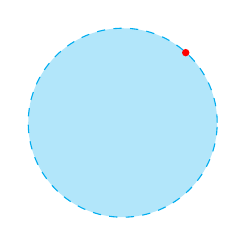
\begin{tikzpicture}[=>stealth]
\draw[dashed,cyan](0,0)circle[radius=1.2cm];
\path[fill=cyan,opacity=0.3](0,0)circle[radius=1.2cm];
\draw(0.8,0.89)node[shape=circle,fill=red,scale=0.01cm]{};
\end{tikzpicture}
\end{figure}


















\textbf{\textcolor{red}{Example}}\\
Any point with $\hspace{0.2cm}\left|z\right| = 1\hspace{0.2cm}$ is a limit point of the set $\hspace{0.2cm}\big\{ z \in \mathbb{C}: \hspace{0.2cm} \left|z\right| < 1\big\}$\\


















Consider $\hspace{0.2cm}\big\{ z \in \mathbb{C}: \hspace{0.2cm} \left|z\right| < 1\big\} \cup \big\{ 13 + 20 i\big\} = S\hspace{0.2cm}$ then $13 + 20i\hspace{0.2cm}$ is an isolated point.\\\\






\textbf{\textcolor{red}{Example}}\\
Consider the set $\hspace{0.2cm} S = \big\{ x + iy\in \mathbb{C}: \hspace{0.2cm} x,y\in \mathbb{R}\big\}$. Show that every complex number is a limit point of $S$.\\


\textbf{\textcolor{teal}{Proof}}\\




Let $\hspace{0.2cm} z = x  + i y \in \mathbb{C}$\\
$\lim\hspace{0.1cm} B'(z,\varepsilon) \cap S \neq \emptyset$\\
There are rational numbers $\hspace{0.2cm} x_0,y_0\ni x < x_0 < x + \dfrac{\varepsilon}{\sqrt{2}}\hspace{0.2cm}$ and $\hspace{0.2cm} y < y_0 < y + \dfrac{\varepsilon}{\sqrt{2}}$\\
So $\hspace{0.2cm} x_0 + iy_0 \in S\hspace{0.2cm}$ and $\hspace{0.2cm} x_0 + iy_0 \in B'(z,\varepsilon)$
$$x_0 +iy_0 \in S\cap B'(z,\varepsilon)$$
Hence $z$ is a limit point of $S$\\\\





\textbf{\textcolor{red}{Example}}\\
Consider the set $\hspace{0.2cm} S = \Big\{ \dfrac{1}{k} + i\dfrac{2}{k}\hspace{0.1cm}:\hspace{0.1cm} k \in \mathbb{Z}\Big\}.\hspace{0.2cm}$ We show that 0 is he limit point of $S$.\\



Consider $\hspace{0.2cm} B'(0,\varepsilon) , \hspace{0.2cm} \varepsilon > 0.\hspace{0.2cm}$ So by Archimedean property. $\dfrac{1}{4n} < \dfrac{1}{n} < \varepsilon\hspace{0.2cm}$ to get $$ \dfrac{1}{4n} + \dfrac{i}{2n} \in B'(0,\varepsilon) \cap S$$
So 0 is a limit point of $S$.\\

For $\hspace{0.2cm} z = x + iy\in \mathbb{C}$ and $z$ not of the form $x + 2iy$ for some $x\in \mathbb{R}$ then the $\perp^r$ distance of the point from the line say $\varepsilon_z$ is positive.
Then $\hspace{0.2cm} B(z,\varepsilon_z) \cap S = \emptyset$.
So $z$ is not a limit point of $S$.\\

$\implies\hspace{0.2cm}$ If $z = x + iz_x \in\mathbb{C}\hspace{0.2cm} x> 1$ or $x < -1 \hspace{0.2cm} (x \in \mathbb{R})$ then take $\varepsilon_z = \left|x - 1\right|$ or $\varepsilon_z = \left|x + 1\right|$ respectively $$B'(z, \varepsilon_z) \cap S = \emptyset$$

$\implies\hspace{0.2cm}$ If $z$ is of the form $x + 2ix, \hspace{0.2cm} - 1 \leq x \leq 1$ and $z\not \in S$ then there are integers 
$$ k, \hspace{0.3cm} k + 1 \ni \dfrac{1}{k + 1} < x < \dfrac{1}{k}$$









Pick $\hspace{0.2cm} \varepsilon_z = \min\Big\{ \left|x - \dfrac{1}{k + 1}\right|, \left|x - \dfrac{1}{k}\right|\Big\}$
$$B(z,\varepsilon_z) \cap S = \emptyset$$


$\implies\hspace{0.2cm}$ If $z = x + 2ix$ and $-1\leq x \leq 1$ and $z \in S$ there is a $\hspace{0.2cm} k\ni x = \dfrac{1}{k}$
$$\text{take}\hspace{0.5cm} \varepsilon_2 = \dfrac{1}{\big(k + 1\big)2}\hspace{2cm} \Bigg(\dfrac{1}{k},\dfrac{1}{k + 1}\Bigg)$$
$B'(z,\varepsilon_z) \cap S = \emptyset$\\
Any point  $\hspace{0.2cm} z \in \mathbb{C}/\{0\}\hspace{0.2cm}$ is not a limit point and $\hspace{0.2cm} z \in \mathbb{C}/\{0\} \cap S = S\hspace{0.2cm}$ is an isolated point of $S$.\\\\






\textbf{\textcolor{teal}{Definition}}\\
The closure of a set $\hspace{0.2cm} S\subseteq \mathbb{C},\hspace{0.2cm}$ denoted by $\overline{S}$, is the union of $S$ and the set of all limit points of $S$.\\\\





\textbf{\textcolor{red}{Example}}\\
(Show that every point in $\mathbb{C}$ is a limit point of $\hspace{0.3cm} S = \big\{x + iy:\hspace{0.2cm} x\in \mathbb{Q},\hspace{0.2cm} y \in \mathbb{Q}\big\}$
$$\overline{S} = S\cup \mathbb{C} = \mathbb{C}$$

E.g $\hspace{0.2cm} S = \Big\{ \dfrac{1}{k} + i\dfrac{2}{k}:\hspace{0.2cm} k \in \mathbb{Z}\Big\}$\\

$\overline{S} = \Big\{ \dfrac{1}{k} + i\dfrac{2}{k}:\hspace{0.2cm} k \in \mathbb{Z}\Big\}\cup \big\{0\big\}$\\\\






\textbf{\textcolor{teal}{Proposition}}\\
Let $S\subseteq \mathbb{C}$. $\overline{S}$ is a closed set in $\mathbb{C}$.\\


\textbf{\textcolor{teal}{Proof}}\\
Let $z\in \overline{S}^c$ so $z\in S\Big(\therefore \overline{S}\supseteq S\Big)$. Also $z$ is not a limit point of $S$ which implies\\ $\exists \hspace{0.1cm} \varepsilon > 0 \ni B(z;\varepsilon) \cap S  = \emptyset$. (We want to show that $B(z;\varepsilon)\cap \overline{S} = \emptyset$)\\
Suppose that $\hspace{0.1cm} B'(z; \varepsilon) \cap \overline{S}\neq \emptyset\hspace{0.2cm}$ then there is a limit point of $S$ in $B'(z;\varepsilon)$ say $w$ $$\left|w - z\right| < \varepsilon$$
Let $0 < \delta < \varepsilon - \left|w - z\right|$. Then $B'(w,\delta) \cap S \neq \emptyset$. ($\therefore w$ is a limit point)\\
$\implies\hspace{0.2cm} B'(z;\varepsilon) \cap S\neq \emptyset\hspace{0.1cm}$ which is a contradiction.  So $$B(z;\varepsilon) \cap \overline{S} = \emptyset \implies B(z;\varepsilon) \subseteq \overline{S}^c$$
$\implies\hspace{0.2cm} \overline{S}^c\hspace{0.1cm}$ is open in $\mathbb{C} \implies \overline{S}$ is a closed set.\\\\\\












\textbf{\textcolor{teal}{Proposition}}\\
Let $\hspace{0.2cm} S\subseteq \mathbb{C}$, then the following are equivalent

\begin{enumerate}
\item[(i).] $S$ is closed (in $\mathbb{C}$)
\item[(ii).] $S$ contains all its limits points.
\item[(iii).] $\overline{S} = S$\\
\end{enumerate}





\textbf{\textcolor{teal}{Proof}}\\

(i) $\hspace{0.2cm} \implies\hspace{0.2cm}$ (ii) $\hspace{0.2cm} \implies \hspace{0.2cm}$ (iii) $\hspace{0.2cm}\implies\hspace{0.2cm}$ (i)\\

(ii) $\hspace{0.2cm} \implies \hspace{0.2cm}$ is by definition of closure  $\big(\hspace{0.2cm} \overline{S} = S\cup \big\{\text{limit points of}\hspace{0.1cm} S\big\}\hspace{0.2cm} = S\big)$.\\

(iii) $\hspace{0.2cm} \implies \hspace{0.2cm}$ (i) $\hspace{0.1cm}\overline{S}$ is a closed set and if $S = \overline{S}$, $S$ is a closed set.\\

(i) $\hspace{0.2cm} \implies \hspace{0.2cm}$ (ii) Suppose $S$ is closed. (will show: limit points of $S$ cannot be in $S^c$).
Suppose $z \in S^c$ is a limit point of $S$. Since $S^c$ is open $\hspace{0.2cm} \exists\hspace{0.1cm} \varepsilon > 0 \ni B(z; \varepsilon ) \subseteq S^c$. $\implies \hspace{0.2cm} B(z;\varepsilon) \cap S = \emptyset$ which contradicts the assumption that $z$ is a limit point.\\
$\implies\hspace{0.1cm} S$ contains all its limit points.\\\\\














\textbf{\textcolor{teal}{Definition}}\\
\textbf{\textcolor{teal}{Interior Point:}} Let $S\subseteq \mathbb{C}$. A point $z\in S$ is called an interior point of $S$, if there is $\hspace{0.2cm} \varepsilon > 0 \ni B(z; \varepsilon) \subseteq S$.\\

\begin{enumerate}
\item Every point of an open set is an interior point.
\item Consider $\hspace{0.2cm} S = \big\{ x+ iy\in \mathbb{C}:\hspace{0.2cm} x,y \in \mathbb{Q}\big\}$\\
Then no point of $S$ is an interior point.\\

\end{enumerate}




\textbf{\textcolor{teal}{Fact}}\\
Every interior point is a limit point.\\









Boundary point\\










$B(0;1) = \big\{z: \hspace{0.2cm}\left|z\right| < 1\big\}$\\

$\big\{z: \hspace{0.2cm} \left|z\right| = 1\big\}\hspace{0.2cm}$ boundary of $B(0,1)$.\\\\\\














\textbf{\textcolor{teal}{Definition}}\\
Let $\hspace{0.1cm} S\subseteq \mathbb{C}$. A point $z \in \mathbb{C}$ is called a boundary point of $S$ if $\hspace{0.2cm} B(z,\varepsilon) \cap S \neq \emptyset\hspace{0.2cm}$ and $\hspace{0.2cm} B(z,\varepsilon) \cap S^c \neq \emptyset\hspace{0.2cm} \forall \varepsilon > 0$.\\

( So every $\varepsilon -$ neighbourhood of $z$ contains points from $S$ and from $S^c$).\\


Every point of $\mathbb{C}$ is a boundary point of $S$.\\













\textbf{\textcolor{teal}{Exercise}}\\
What is the boundary of $\hspace{0.3cm} S = \big\{ z:\hspace{0.2cm}\left|z\right| < 1\big\} \cup \big\{n + 0i: \hspace{0.2cm} n\in \mathbb{Z}\big\}$\\ Find the limit points and interior points of $S$.\\\\\\


\textbf{\textcolor{teal}{Exterior Points:}}\\
A point $z\in \mathbb{C}$ is called an exterior point to a set $S\subseteq \mathbb{C}$ there is an $\hspace{0.2cm} \varepsilon > 0 \ni B(z,\varepsilon) \cap S = \emptyset$.\\\\


\textbf{\textcolor{teal}{Facts}}
\begin{enumerate}
\item Every interior point is a limit point but limit point need not to be an interior point.
\item Isolated points are never interior points and interiors never isolated.
\item Every boundary point of a set $S$ is an isolated point or a limit point.
\item Every limit point need not be a boundary point.\\\\\\
\end{enumerate}












{\color[wave]{485}\subsection{Compactness}}

\textbf{\textcolor{teal}{Definition}}\\
A set $\hspace{0.1cm} S\subseteq \mathbb{C}\hspace{0.1cm}$ is said to be bounded if there is an $\hspace{0.2cm}M > 0 \ni \left|z\right| < M\hspace{0.2cm} \forall z \in S$.\\\\


















\textbf{\textcolor{teal}{Definition}}\\
Let $\hspace{0.2cm} S\subseteq \mathbb{C}$. An open covering of $S$ is a collection of open sets $\hspace{0.2cm} G \ni \bigcup\limits_{g \in G}g\supseteq S$.\\\\



\textbf{\textcolor{teal}{Definition}}\\
A set $\hspace{0.1cm} S\subseteq \mathbb{C}\hspace{0.1cm}$ is said to be compact if every open covering of $S$ has a finite sub-cover.\\\\



\textbf{\textcolor{red}{Example}}\\

$B(0; 1) \hspace{0.5cm} G = \big\{B(0; r): \hspace{0.2cm} r \in [ 0,1) \subseteq \mathbb{R}\big\}$\\

$\bigcup\limits_{r\in [0,1)}B(0; r) \supset B(0; 1)$\\

No subcollection of $G$ contains $\hspace{0.1cm} B(0; 1)$\\


E.g $\hspace{0.2cm} \big\{ n + i0: \hspace{0.1cm} n \in \mathbb{N}\big\} \subset \mathbb{C}$\\















$G = \big\{ B(0; n):\hspace{0.1cm} n\in \mathbb{N}\big\}$\\

$B(0; 2)\hspace{0.6cm} B(0; n)\hspace{0.7cm} B(0; n- 1)$\\\\\\








\textbf{\textcolor{teal}{Theorem: (Heine - Borel)}}\\
A set $\hspace{0.2cm} S \subseteq \mathbb{C}\hspace{0.2cm}$ is compact if and only if it is closed and bounded in $\mathbb{C}$.\\\\



\textbf{\textcolor{red}{Example}}
\begin{enumerate}
\item Unit circle in $\mathbb{C}$ is compact
\end{enumerate}
\vspace{1cm}










\textbf{\textcolor{teal}{Cantor's Theorem:}}\\
Let $\hspace{0.1cm} K_j'$s be compact subsets of $\mathbb{C},\hspace{0.1cm} j \in \mathbb{N}\hspace{0.2cm}$ with $\hspace{0.2cm} K_1\supset K_2\supset K_3\supset \cdots\cdots\hspace{0.2cm}$ Then $\bigcap\limits_{j= 1}^{\infty}K_j\hspace{0.2cm}$ is nonempty.\\

\textbf{\textcolor{teal}{Proof}}\\
Suppose that $\hspace{0.1cm} \bigcap\limits^{\infty}_{j = 1} K_j\hspace{0.2cm}$ is empty. Then $\hspace{0.2cm} G = \big\{K^c_j : \hspace{0.1cm} j\in \mathbb{N}\big\},\hspace{0.5cm} \mathbb{C} = \bigcup\limits^{\infty}_{j= 1}K^c_j\hspace{0.1cm}$ so that $\hspace{0.1cm}K_1\subset \bigcup\limits^{\infty}_{j = 1} K^c_j$\\
Since $K_1$ is compact, there are numbers $$\hspace{0.2cm} j_1, \hspace{0.2cm} j_2,\cdots\cdots\cdots, j_n,\hspace{0.5cm} j_1< j_2< \cdots\cdots\cdots < j_n \hspace{0.3cm} \ni\hspace{0.3cm} K_1 \subset \bigcup\limits^n_{m = 1}K^c_{j_m} \subset K^c_{j_{n+1}}$$
$$\Big(\therefore\hspace{0.5cm} K_{j_{n+1}} \subset K_{j_n} \subset \cdots\cdots\cdots \subset K_{j_1}\Big)$$
$\implies\hspace{0.2cm} K_1 \cap K_{j_{n+1}} = \emptyset$. Thus a contradiction to the given hypothesis. So $\bigcup\limits^{\infty}_{j = 1}K_j\hspace{0.1cm}$ has to be nonempty.\\\\\\





\textbf{\textcolor{teal}{Proposition}}\\
A closed subset of a compact set is compact.\\\\\\














{\color[wave]{485}\subsection{Connectedness}}

\textbf{\textcolor{teal}{Definition}}\\
A set $S\subseteq \mathbb{C}$ is said to be connected if its not contained in the union of two disjoint nonempty open subsets of $\mathbb{C}$ which have a non trivial intersection with $S$\\


$\big[ G_1 \cup G_2,\hspace{0.3cm} G_1\neq \emptyset, \hspace{0.3cm} G_1\cap G_2 = \emptyset\hspace{0.3cm}G_1$ and $G_2$ are open. $\hspace{0.2cm} G_1\cap S \neq \emptyset,\hspace{0.3cm} G_2\cap S \neq \emptyset\big]$\\\\












An open connected nonempty subset of $\mathbb{C}$ is called a region or a domain.\\\\




\textbf{\textcolor{teal}{Proposition}}\\
Let $G$ be a nonempty open subset of $\mathbb{C}$. Then $G$ is a region if and only i any two points of $G$ can be connected by a polygonal path.\\

\textbf{\textcolor{teal}{Proof}}\\

Suppose that $G$ is a region. Fix $a\in G$ and let $G_1 = \big\{z\in G:\hspace{0.1cm}$ there is a polygonal path from $a$ to $z$ in $G\big\}$.\\
Let $G_2 = G/G_1\hspace{0.2cm} (G_1\cup G_2 = G \implies$ either $G_1 = \emptyset$ or $G_2 = \emptyset)$.\\
Suppose $z\in G$, then since $G_1\subset G$ and $G$ is open then there is  an $\hspace{0.2cm} r> 0 \ni B(z;r)\subset G_1$. Since $a$ and $z$ are connected by a polygonal path, we can extended this path to any point $\hspace{0.2cm} w \in B(z; r)\hspace{0.2cm}$ by joining an additional segment joining $z$ and $w$.\\
So $\hspace{0.2cm}w \in B(z; r)\hspace{0.2cm}$ is such that $\hspace{0.1cm} w \in G$, so $\hspace{0.2cm} B(z; r) \subset G_1 \implies G_1\hspace{0.2cm}$ is open. Likewise $G_2$ is open.\\
$G_1\cup G_2 = G\hspace{0.3cm} G_1, G_2$ are open and $\hspace{0.1cm} G_1\cap G_2 = \emptyset \implies$ either $G_1 = \emptyset$ or $G_2 = \emptyset$. We know that $\hspace{0.2cm} G_1 \neq \emptyset$ so $G_2 = \emptyset\hspace{0.2cm}$ i. e $\hspace{0.1cm} G_1 = G$.\\\\\\


















{\color[wave]{485}\subsection{Sequences}}

\textbf{\textcolor{teal}{Definition}}\\
A sequence of complex numbers is an ordered list of complex numbers such that corresponding to each natural number $n$ there is an $n^{\text{th}}$ number in the list $a_n$. Denoted by $(a_n),\hspace{0.2cm}\big\{a_n\big\}^{\infty}_{n = 1}$\\\\



\textbf{\textcolor{teal}{Definition}}\\
A sequence $(a_n)$ is said to have a limit $L$, if given $\varepsilon > 0$ there is a corresponding\\ $n_0 \in \mathbb{N} \ni \forall n\hspace{0.1cm}\geq n_0, \hspace{0.2cm} \left|a_n - L\right| < \varepsilon$.\\\\














\textbf{\textcolor{teal}{Definition}}\\
A sequence is said to be convergent if it has a limit and is said to be ``not convergent'' if it has no limit.\\


A sequence is said to diverge if given $M> 0$ there is an $\hspace{0.2cm} n_0 \in \mathbb{N} \ni \forall n\hspace{0.1cm} \geq n_0 \hspace{0.2cm} \left|a_n\right| > M$.\\\\









{\color[wave]{485}\textbf{Cauchy's Criterion}}\\
A sequence $(a_n)$ is convergent in $\mathbb{C}$ if and only if given $\varepsilon > 0$ there is an\\ $\hspace{0.2cm} n_0 \in \mathbb{N} \ni \forall n, m\geq n_0, \hspace{0.2cm} \left|a_m - a_n\right| < \varepsilon$.\\\\



{\color[wave]{485}\textbf{Bolzano - Weistrass Theorem}}\\
An infinite subset of a compact set has a limit point.\\















\pagebreak
{\color[wave]{485}\section{Complex Functions}}

{\color[wave]{485}\subsection{Functions}}

\textbf{\textcolor{teal}{Definition}}\\
A complex  valued function of a complex variable (complex function) is a rule that assigns a unique complex number $w$ to each complex number $z$ belonging to a set $D$.\\


\textbf{\textcolor{red}{Example}}\\
$f(z) = z^2 \hspace{0.3cm} \forall z \in \mathbb{C}$\\

Here $D = \mathbb{C}$\\

$f(3 + i) = (3  + i)^2  = 8 + 6i$\\

$* D$ is called the domain of the complex function\\

$*$ The set $\{ f(z): \hspace{0.1cm} z \in D\}$ is called the range of the complex function.\\

$* z \in  D$ is a point in $D$ and $f(z)$ is called the image of the point $z$ under $f$.\\\\



\textbf{\textcolor{teal}{Notation:}}\\
$f: D \longrightarrow \mathbb{C}$ means that $f$ is function (complex) with domain $D$.\\\\



\textbf{\textcolor{red}{Examples}}
\begin{enumerate}
\item \textit{Constant functions:}  $f: \mathbb{C}\longrightarrow \mathbb{C}$ given by $f(z)  = C$ where $C$ is a fixed constant
\item \textit{Polynomial function:} $f: \mathbb{C}\longrightarrow \mathbb{C}$ defined by $$f(z) = a_n z^n + a_{n - 1}z^{n - 1} + \cdots\cdots + a_0$$ Here $n$ is a non negative integer and $a_n , \cdots\cdots\cdots, a_0$ are complex constants $(a_n\neq 0)$.\\

\textbf{\textcolor{red}{Example}}\\
$f(z ) = 3z^2 - (2 + i)z + 13 - \sqrt{2}i$\\
Here the highest power of $z$ carrying a non zero coefficient is 2. $\implies f(z)$ is a second degree polynomial.
\item \textit{Rational function:} Let $p(z)$ and $q(z)$ be polynomial functions where $q(z) \neq 0$. Then $f(z) = \dfrac{p(z)}{q(z)}$ is called a rational function. The domain of $z$ is the set $\{z\in \mathbb{C}:\hspace{0.2cm}q(z)\neq 0\}$\\


\textbf{\textcolor{red}{Examples}}
\begin{enumerate}
\item $f(z) = \dfrac{az + b}{cz + d}$ where $a, b, c, d\in \mathbb{C}$ and $c$ and  $d$ are not both zeroes is a rational function.\\
$f$ is called a linear fractional transformation.\\
Domain of $f= \begin{cases}
\mathbb{C} - \big\{-d/c\big\} & \text{if}\hspace{0.2cm} c\neq 0\\
\mathbb{C} & \text{if}\hspace{0.3cm} c = 0\\
\end{cases}$

\item $g(z) = \dfrac{3z^4 - (2 + i)z}{2z - 3i}\hspace{0.6cm}\forall z \in \mathbb{C} - \Big\{\dfrac{3i}{2}\Big\}$\\\\ 
\end{enumerate}
\end{enumerate}





\textbf{\textcolor{teal}{Real and Imaginary Parts of a Complex Function}}\\

Let $f(z) = z^3$ for $z \in \mathbb{C}$
$$f(x + iy) = (x + iy)^3 = x^3 - 3xy^2 + i(3x^2y - y^3)$$

$\implies \hspace{0.2cm} x^3 - 3xy^2$ is the real part of a function $f$\\

$\implies\hspace{0.2cm} 3xy - y^3$ is the imaginary part of a function $f$.\\

In general $f: D\longrightarrow \mathbb{C}$ is function and  $$\hspace{0.2cm} \boxed{f(x + iy) = u(x,y) + iv(x,y)\hspace{0.2cm} , \hspace{0.2cm} \forall x + iy \in D}$$ Then $u(x,y)$ is called the real part of $f$ and $v(x,y)$ is called the imaginary part of $f$.\\\\\





\textbf{\textcolor{teal}{Visualizing Complex Functions}}\\

\textbf{\textcolor{red}{Examples}}\\
$f: \mathbb{C}\longrightarrow \mathbb{C}$ defined by $f(z) = z + b$ ( $b$ is a fixed complex number) $D = \mathbb{C}$

% \DIAGRAM 1

\begin{figure}[H]
\centering
\begin{tikzpicture}[=>stealth]
\draw[-Stealth](-1.5,0)--(3,0);
\draw[-Stealth](0,-0.5)--(0,3);
\draw[dashed,cyan](0,0)--(1.5,0)--(1.5,1.5)--(0,1.5)--cycle;
\draw(1.5,1.5)node[shape=circle,fill=cyan,scale=0.01cm]{}
(0,0)node[shape=circle,fill=cyan,scale=0.01cm]{}
(1.5,1.5)node[right]{$b=b_1+ib_2$}
(0.75,-0.2)node[below]{$b_1$}
(-0.1,0.75)node[left]{$b_2$};
\draw[<->,red](0,-0.2)--(1.5,-0.2);
\draw[<->,red](-0.1,0)--(-0.1,1.5);
\draw[thick,red,-Stealth](4.5,1)--node[sloped,above,black]{$f$}(6.5,1);
\draw[-Stealth](8,0)--(12,0);
\draw[-Stealth](9,-0.5)--(9,3);
\draw(11,2.5)node[shape=circle,fill=teal,scale=0.01cm]{}
(11,1)node[shape=circle,fill=teal,scale=0.01cm]{}
(11,1)node[right]{$f(0)$}
(11,2.5)node[right]{$f(x+iy)$};
\end{tikzpicture}
\end{figure}


$f(0)=0+b=b^*$\\
$f(x+iy)= x +iy+ b_1 + ib_2 = (x +b_1)+i(y+ b_2)$







\vspace{1cm}
% DIAGRAM 2



\begin{figure}[H]
\centering
\begin{tikzpicture}[=>stealth]
\draw[-Stealth](-1,0)--(3,0);
\draw[-Stealth](1,-2)--(1,2);
\draw[thick,cyan](1,0)circle[radius=1.2cm];
\draw(2,-0.66)node[right]{$|z|=1$}
(1,0)node[shape=circle,fill=red,scale=0.01cm]{};
\draw[thick,red,-Stealth](4.5,1)--node[sloped,above,black]{$f$}(6.5,1);
\draw[-Stealth](8,0)--(12,0);
\draw[-Stealth](9,-0.5)--(9,3);
\draw[thick,teal](10.2,1.2)circle[radius=1.2cm];
\draw(10.2,1.2)node[shape=circle,fill=red,scale=0.01cm]{}
(10.2,1.2)node[below]{$b$}
(11.4,1.2)node[right]{$|z-b|=1$};
\end{tikzpicture}
\end{figure}

$$f\big(\big\{z:|z|=1\big\}\big)=\big\{z:|z-b|=1\big\}$$

















\textbf{\textcolor{red}{Example}}\\
$f(z) = az$ for $z \in \mathbb{C}$ where $a$ is a fixed non zero constant.\\

If $a = r(\cos \theta + i\sin \theta)$ and if $z = \rho ( \cos \phi + i \sin \phi)$. Then $f(z) = \rho r ( \cos (\theta + \phi) + i \sin (\theta + \phi))$\\

% DIAGRAM 3


\begin{figure}[H]
\centering
\begin{tikzpicture}[=>stealth]
\draw[-Stealth](-1.5,0)--(3,0);
\draw[-Stealth](0,-0.5)--(0,3);
\draw[thick,cyan](0,0)--node[above,sloped,black]{$\rho$}(3,2);
\draw(3,2)node[shape=circle,fill=cyan,scale=0.01cm]{}
(3,2)node[right]{$z$};
\coordinate (a) at (0.5,0);
\coordinate (b) at (0,0);
\coordinate (c) at (0.5,0.33);
\draw
pic[draw=cyan,thick,angle radius = 0.8cm, angle eccentricity=1.3,"$\phi$"]{angle=a--b--c};
\draw[thick,red,-Stealth](4.5,1)--node[sloped,above,black]{$f$}(6.5,1);
\draw[-Stealth](8,0)--(12,0);
\draw[-Stealth](9,-0.5)--(9,3);
\draw[thick,teal](9,0)--node[above,sloped,black]{$\rho r$}(10.5,3);
\draw(10.5,3)node[shape=circle,fill=teal,scale=0.01cm]{};
\coordinate (A) at (9.5,0);
\coordinate (B) at (9,0);
\coordinate (C) at (9.5,1);
\draw
pic[draw=teal, thick, angle radius=0.8cm, angle eccentricity = 1.6,"$\phi + \theta $"]{angle=A--B--C};
\end{tikzpicture}
\end{figure}













\textbf{\textcolor{red}{Examples:}}\\
$f(z) = az + b\hspace{0.3cm} z \in \mathbb{C}$ can be visualized as follows:
\begin{enumerate}
\item $z$ is elongated  (or contracted) by a factor $\left|a\right|$.
\item Then it is rotated (in the counter clockwise direction) by angle $\operatorname{arg}(a)$
\item Then it is translated by a vector $b$.\\\\
\end{enumerate}




\textbf{\textcolor{red}{Example}}\\
$f(z) = z^3\hspace{0.3cm} \forall z \in \mathbb{C}$\\

$f[r(\cos \theta + i \sin \theta ) ] = r^3(\cos 3\theta + i \sin 3\theta)$\\

So $f$ can be visualized as follows:
\begin{enumerate}
\item Given a complex number $z$ with modulus $r$ and argument $\theta$,  first elongate vector $z$ as $r^3$
\item Then rotate $z$ upto the ray $\phi = 3\theta$\\

Let $z = 1 + i = \sqrt{2} \Big(\cos \dfrac{\pi}{4} + i \sin \dfrac{\pi}{4}\Big)$\\

% DIAGRAM 4


\begin{figure}[H]
\centering
\begin{tikzpicture}[=>stealth]
\draw[-Stealth](-1.5,0)--(3,0);
\draw[-Stealth](0,-0.5)--(0,3);
\draw[thick,cyan](0,0)--(2,2);
\draw(2,2)node[shape=circle,fill=cyan,scale=0.01cm]{}
(2,2)node[right]{$1 + i$};
\coordinate (a) at (0.5,0);
\coordinate (b) at (0,0);
\coordinate (c) at (0.5,0.5);
\draw
pic[draw=cyan,thick,angle radius = 0.8cm, angle eccentricity=1.3,"$\dfrac{\pi}{4}$"]{angle=a--b--c};
\draw[thick,red,-Stealth](4.5,1)--(6.5,1);
\draw[-Stealth](8,0)--(12,0);
\draw[-Stealth](9,-0.5)--(9,3);
\draw[thick,teal](9,0)--(12,3);
\draw(12,3)node[shape=circle,fill=teal,scale=0.01cm]{}
(12,3)node[right]{$(\sqrt{2})^3$};
\coordinate (A) at (9.5,0);
\coordinate (B) at (9,0);
\coordinate (C) at (9.5,0.5);
\draw
pic[draw=teal, thick, angle radius=0.8cm, angle eccentricity = 1.6,"$\dfrac{\pi}{4}$"]{angle=A--B--C};
\end{tikzpicture}
\end{figure}




\begin{figure}[H]
\centering
\begin{tikzpicture}
\draw[-Stealth](-3,0)--(2,0);
\draw[-Stealth](0,-1)--(0,3);
\draw[thick,teal](0,0)--(-3,3);
\draw(-3,3)node[shape=circle,fill=teal,scale=0.01cm]{}
(-3,3)node[left]{$(\sqrt{2})^3\big(\cos\frac{\pi}{4}+i\sin\frac{\pi}{4};\big)$};
\coordinate (a) at  (0.5,0);
\coordinate (b) at (0,0);
\coordinate (c) at (-0.5,0.5);
\draw
pic[draw=teal, thick,angle radius = 0.8cm, angle eccentricity = 1.5, "$\dfrac{3\pi}{4}$"]{angle = a--b--c};
\draw[thick,red,-Stealth](-6,1)--(-4,1);
\end{tikzpicture}
\end{figure}

\end{enumerate}












{\color[wave]{485}\subsection{Limits of Complex Functions}}

\textbf{\textcolor{teal}{Definition}}\\
Let $D\subseteq \mathbb{C}$. Let $f: D\longrightarrow \mathbb{C}$ be a function and let $z_0$ be a limit point of $D$. A complex number $L$ is said to be a limit of the function $f$ as $z$ approaches $z_0$ if $\forall \varepsilon > 0 \hspace{0.1cm}\exists\hspace{0.1cm} \delta > 0 \ni \left|f(z) - L\right|  < \varepsilon$ whenever $z\in D$ and $0 < \left|z - z_0\right| < \delta$.\\




If $\forall \varepsilon > 0 \hspace{0.1cm}\exists\hspace{0.1cm} \delta > 0 \ni$ whenever $z \in D \cap B'(z_0,\delta), \hspace{0.2cm} f(z) \in B(L;\varepsilon)$
$$\lim\limits_{z \rightarrow z_0} f(z) = L$$\\






\textbf{\textcolor{red}{Example}}\\

$f(z) = \begin{cases}
3z^2, & \left|z\right| < 1\\\\
3, & \left|z\right|= 1\\
\end{cases}$\\\\

$f: \overline{B}(0;1) \longrightarrow \mathbb{C}$\\

$\lim\limits_{z \rightarrow 1} f(z)  = \mathbb{C}$\\

$\lim\limits_{z \rightarrow z_0} f(z)$ does not exist for any $z_0$ with $\left|z_0\right| = 1$ and $z_0 \neq \pm 1$.\\\\\\








\textbf{\textcolor{red}{Example}}\\
Show that $\lim\limits_{z \rightarrow 0}\dfrac{z}{\overline{z}}$ does not exist.\\



\text{\textcolor{red}{Solution}}\\
We show that this limit does not exist by finding two different ways of letting $z$ approach 0 that yields different values of $\lim\limits_{z \rightarrow 0}\dfrac{z}{\overline{z}}$.\\
First let $z$ approach  0 along the real axis, that is $z = x + 0i$. Then for these points, we have  
$$\lim\limits_{z \rightarrow 0}\dfrac{z}{\overline{z}}= \lim\limits_{z \rightarrow 0}\dfrac{x + i0}{x - i0} = \lim\limits_{z \rightarrow 0} 1 = 1$$
On the other hand, if we let $z$ approach 0 along the imaginary axis then $z = 0  + iy$. And for this approach, we have  
$$\lim\limits_{z \rightarrow 0}\dfrac{z}{\overline{z}} = \lim\limits_{z \rightarrow 0}\dfrac{0 + iy}{0 - iy} = \lim\limits_{z \rightarrow 0} (-1) = -1$$ 
Hence the two limits are different and we conclude that $\lim\limits_{z \rightarrow 0}\dfrac{z}{\overline{z}}$ does not exist.\\\\






\textbf{\textcolor{red}{Example}}\\
Use the $\varepsilon - \delta$ definition to show that $\lim\limits_{z \rightarrow (1 + i)}(2 + i) z = 1 + 3i$.\\



\text{\textcolor{red}{Solution}}\\
According to the definition, $\lim\limits_{z \rightarrow (1 + i)}(2 + i) z = 1 + 3i$ if for every $\varepsilon > 0$, there exist $\delta > 0$ such that $\left|(2 + i)z - (1 + 3i)\right| < \varepsilon$ whenever $0 < \left|z - (1 + i)\right| < \delta$. To do this, we need to find the value of $\delta$ for any given $\varepsilon$, that is given any value of $\varepsilon$, we must find a real number $\delta > 0$ such that if $0 < \left|z - (1 + i)\right| < \delta$, then $\left|(2 + i) z - (1 + 3i)\right| < \varepsilon$.

\begin{align*}
\text{Now}\hspace{0.5cm} \left|f(z) - L\right| & = \left|(2 + i)z - (1 + 3i)\right| = \left|(2 + i) -\Big(z - \dfrac{1 + 3i}{2 + i}\Big)\right|\\
& = \left|2 + i\right|\hspace{0.1cm}\left|z - \dfrac{1 + 3i}{2 + i}\right|
\end{align*}

Now $\left|2 + i\right| = \sqrt{5}$ and $\dfrac{1 + 3i}{2  + i} = 1 + i$. So we have


\begin{align*}
\left|f(z) - L\right| & = \sqrt{5}\hspace{0.1cm}\left|z - (1 + i)\right|  < \varepsilon\\
& \implies \left|z - (1 + i)\right| < \dfrac{\varepsilon}{\sqrt{5}}
\end{align*}

Then we can choose $\delta = \dfrac{\varepsilon}{\sqrt{5}}$\\\\\\



\textbf{\textcolor{teal}{Theorem}}\\
Suppose that $f(z) = u(x,y) + i v(x,y), \hspace{0.3cm} z_0 = x_0 + i y_0$ and  $L = u_0 + i v_0$. Then $\lim\limits_{(x,y) \rightarrow z_0}f(z) = L$ if and only if $\lim\limits_{(x,y)\rightarrow (x_0, y_0)} u(x,y) = u_0$ and $\lim\limits_{(x,y)\rightarrow (x_0, y_0)} v(x,y) = v_0$\\\\\\



\textbf{\textcolor{red}{Example}}\\
Use the theorem to compute $\lim\limits_{z \rightarrow (1 + i) }(z^2 + i)$\\


\text{\textcolor{red}{Solution}}\\
Since $f(z) = (z^2 + i) = (x + iy)^2 + i = x^2 - y^2 + (2xy + 1)i$. So let $u(x,y) = x^2 - y^2$ and $v(x,y) = 2xy + 1$ and $z_0 = 1 + i$, identifying $x_0 = 1;\hspace{0.2cm} y_0 = 1$\\
We find $u_0$ and $v_0$ by computing these two real parts. $u_0 = \lim\limits_{(x,y) \rightarrow (1,1)} (x^2 - y^2 )$ and\\ $v_0 = \lim\limits_{(x,y) \rightarrow (1,1)} (2xy + 1)$. Hence
\begin{align*}
u_0 & = \lim\limits_{(x,y) \rightarrow (1,1)} (x^2 - y^2 ) = 1^2 - 1^2 = 0\\\\
v_0 & = \lim\limits_{(x,y) \rightarrow (1,1)} (2xy + 1) = 2 + 1 = 3
\end{align*}
So $L = u_0 + iv_0 = 0 + 3i = 3i$\\\\\\




\textbf{\textcolor{teal}{Theorem}}\\
Suppose that $f$ and $g$ are complex functions. If $\lim\limits_{z\rightarrow z_0} f(z) = L$ and $\lim\limits_{z\rightarrow z_0} g(z) = M$, then
\begin{enumerate}
\item $\displaystyle{\lim\limits_{z\rightarrow z_0}C( f(z)) = CL}\hspace{0.1cm},\hspace{0.2cm}$ a complex number.
\item $\displaystyle{\lim\limits_{z\rightarrow z_0} (f(z)\pm g(z)) = L\pm M}$
\item $\displaystyle{\lim\limits_{z\rightarrow z_0} (f(z)\cdot g(z) )= L\cdot M}$
\item $\displaystyle{\lim\limits_{z\rightarrow z_0} \dfrac{f(z)}{g(z)} = \dfrac{L}{M}}$\\\\
\end{enumerate}






\textbf{\textcolor{blue}{Exercise}}\\
Compute the following limits
\begin{enumerate}
\item $\displaystyle{\lim\limits_{z \rightarrow i}\dfrac{(3 + i)z^4 - z^2 + 2z}{z + 1}}$
\item $\displaystyle{\lim\limits_{z \rightarrow (1 + \sqrt{3}i)} \dfrac{z^2 - 2z + 4}{z - 1 -\sqrt{3}i}}$\\\\\\
\end{enumerate}




\textbf{\textcolor{teal}{Limits Involving Infinity}}\\
We can allow $L$ to be $\infty$.\\



\textbf{\textcolor{teal}{Definition}}\\
Let $D\subseteq \mathbb{C}$ and let $f: D\longrightarrow \mathbb{C}$ and let $z_0$ be a limit point of $D$. We say that $\hspace{0.2cm}\displaystyle{\lim\limits_{z\rightarrow z_0} f(z) = \infty}\hspace{0.2cm}$ if given $M> 0 \hspace{0.1cm}\exists \hspace{0.1cm}\delta > 0 \ni \forall z \in D$ and $0 < \left|z - z_0\right| < \delta,\hspace{0.2cm} \left|f(z)\right|> M$ ( is arbitrary large).\\

We say $\displaystyle{\lim\limits_{z\rightarrow \infty} f(z) = L}$ if given $\varepsilon > 0\hspace{0.1cm}\exists\hspace{0.1cm} M> 0 \ni \left|f(z) - L\right| < \varepsilon$ whenever\\ $z \in \big\{W:\hspace{0.1cm}\left|W\right|> M\big\}\hspace{0.2cm}\left|z\right| > M$.\\\\






\textbf{\textcolor{red}{Example}}\\
Show that $\displaystyle{\lim\limits_{z\rightarrow \infty} \dfrac{3z^2}{(1 + i) z^2 - z + 2} = \dfrac{3}{1 + i}}\hspace{0.1cm},\hspace{0.2cm}$ for $\left|z\right| > M\hspace{0.3cm}$ ($M$ is large).\\

\begin{align*}
\left|\dfrac{3z^2}{(1 + i)z^2 - z + 2} - \dfrac{3}{1 + i}\right| & = \left|\dfrac{3z - 6}{(1 + i) ((1 + i)z^2 - z + 2)}\right|\\\\
& = \left|\dfrac{3/z - 6/z^2}{(1 + i)\Big((1 + i)- \dfrac{1}{z} + \dfrac{2}{z^2}\Big)}\right|\hspace{0.3cm}\cdots\cdots\cdots\hspace{0.5cm} (*)
\end{align*}
$\implies\hspace{0.2cm}\displaystyle{\left|(1 + i) - \dfrac{1}{z} + \dfrac{2}{z^2}\right|\geq \sqrt{2}- \left|\dfrac{1}{z} - \dfrac{2}{z^2}\right|\hspace{0.1cm}}$ when $\left|z\right|\geq M$ then $\dfrac{1}{\left|z\right|} \leq \dfrac{1}{M}$

\begin{align*}
\left|\dfrac{1}{z} - \dfrac{2}{z^2}\right| & \leq \dfrac{1}{M} + \dfrac{2}{M^2}\\\\
\implies \hspace{0.2cm}
-\left|\dfrac{1}{z} - \dfrac{2}{z^2}\right| & \geq -\dfrac{1}{M} - \dfrac{2}{M^2}\\\\
\implies\hspace{0.2cm}
\left|(1 + i)- \dfrac{1}{z} + \dfrac{2}{z^2}\right| & \geq \sqrt{2} +  \dfrac{1}{M} + \dfrac{2}{M^2}
\end{align*}


\begin{align*}
(*)& \leq \dfrac{3/M + 6/M^2}{\sqrt{2}\Big(\sqrt{2} + 1/M + 2/M^2\Big)} = \dfrac{3}{\sqrt{2}}\Bigg(\dfrac{M + 2}{\sqrt{2}M^2 + M + 2}\Bigg)\\
&\leq \dfrac{3}{\sqrt{2}}\cdot \dfrac{2M}{2\sqrt{2}M^2} = \dfrac{3}{2M}\hspace{2cm} (2M \leq \sqrt{2}M^3)
\end{align*}
for large $M \hspace{0.2cm} (*)$ is arbitrary small. Thus the limit.\\\\\





{\color[wave]{485}\subsection{Continuity of Complex Functions}}


\textbf{\textcolor{teal}{Definition}}\\
Let $D\subseteq \mathbb{C}$. A function $f: D \longrightarrow \mathbb{C}$ is said to be continuous at a point $z_0\in D$ if given $\varepsilon > 0 \hspace{0.1cm}\exists \hspace{0.1cm}\delta > 0 \ni \left|f(z) - f(z_0)\right| < \varepsilon$ whenever $\left|z - z_0\right| < \delta$.\\


OR\\

A complex function $f$ is continuous at a point $z_0$ if $\lim\limits_{z\rightarrow z_0}f(z) = f(z_0)$\\\\


\textbf{\textcolor{teal}{Criteria for Continuity at a Point}}\\
A complex function $f$ is continuous at a point $z_0$ if each of the following three conditions hold
\begin{enumerate}
\item  $\lim\limits_{z\rightarrow z_0}f(z) $ exists
\item $f$ is defined at $z_0$ and
\item  $\lim\limits_{z\rightarrow z_0}f(z) = f(z_0)$\\
\end{enumerate}



If a complex function is not continuous at a point $z_0$, then we say that $f$ is discontinuous at $z_0$. For example the function $f(z) = \dfrac{1}{1 + z^2}$ is discontinuous at $z  = i$ and $z = -i$.\\\\





\textbf{\textcolor{teal}{Sequential Definition of Continuity}}\\
Let $D\subseteq \mathbb{C}$. A function $f: D\longrightarrow \mathbb{C}$ is said to be continuous at a point $z_0\in D$ if $\forall \{z_n\}^{\infty}_{n = 1}\ni z_n \in D\hspace{0.1cm} \forall n \in \mathbb{N}\hspace{0.2cm}\& \hspace{0.2cm} z_n \longrightarrow z_0, \hspace{0.2cm} \lim\limits_{z_n \rightarrow 0} f(z_n ) = f(z_0)$.\\\\\\




\textbf{\textcolor{red}{Example}}\\
Determine if $f(z) = z^2 - iz + 2$ is continuous at $z_0 = 1 - i$.\\


\text{\textcolor{red}{Solution}}\\
We must find  $\lim\limits_{z\rightarrow z_0}f(z)$ and    $f(z_0)$. Now\hspace{0.2cm} $\displaystyle{ \lim\limits_{z\rightarrow z_0}f(z) =  \lim\limits_{z\rightarrow (1 - i)}(z^2 - iz + 2) = 1 - 3i}$\\

Furthermore, $f(z_0) = f(1 - i) = (1- i)^2 - i(1 - i) + 2 = 1 - 3i$\\

Since  $\lim\limits_{z\rightarrow z_0}f(z) = f(z_0)$, we conclude that $f(z)$ is continuous at the point $z_0  = 1 -i$.\\\\\\





\textbf{\textcolor{red}{Example}}\\
Show that the principal square root function $f(z) = z^{1/2}$ is discontinuous at $z  = -1$.\\

\text{\textcolor{red}{Solution}}\\
We show that $f(z) = z^{1/2}$ is discontinuous at $z_0 = -1$ by demonstrating that\\  $\lim\limits_{z\rightarrow z_0}f(z) =  \lim\limits_{z\rightarrow -1}z^{1/2}$ does not exists.\\

Recall that the principal square root function is defined by $\displaystyle{z^{1/2} = \left|z\right|^{1/2}\hspace{0.1cm} e^{i\hspace{0.1cm}Arg(z) / 2}}$\\
Now consider $z$ approaching $-1$ along the quarter of the unit circle lying in the second quadrant.

% DIAGRAM F_1

\begin{figure}[H]
\centering
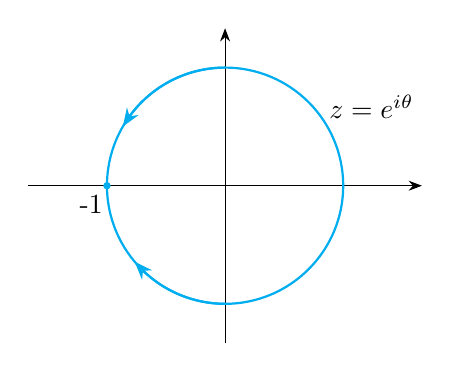
\begin{tikzpicture}[=>stealth]
\draw[-Stealth](-2.5,0)--(2.5,0);
\draw[-Stealth](0,-2)--(0,2);
\draw[thick,cyan](0,0)circle[radius=1.5cm];
\draw(-1.5,0)node[shape=circle,fill=cyan,scale=0.01cm]{}
(-1.7,0)node[below]{-1}
(1.2,1)node[right]{$z=e^{i\theta}$};
\draw[-Stealth,cyan,thick](0,1.5)arc[start angle=90,end angle=150,radius=1.5cm];
\draw[-Stealth,cyan,thick](0,-1.5)arc[start angle=270,end angle=220, radius=1.5cm];
\end{tikzpicture}
\end{figure}
















That is, consider the points $\left|z\right| = 1, \hspace{0.2cm} \dfrac{\pi}{2} < \operatorname{arg}(z) < \pi$. In exponential form, this approach can be described as $z = e^{i\theta}, \hspace{0.3cm} \dfrac{\pi}{2}< \theta < \pi,$ with $\theta$ approaching $\pi$. Thus letting $\left|z\right| = 1$ and letting $Arg(z)  = \theta$ approach $\pi$, we obtain
$$ \lim\limits_{z\rightarrow -1}z^{1/2} = \lim\limits_{z\rightarrow -1}\left|z\right|^{1/2}\hspace{0.1cm}e^{i\hspace{0.1cm}Arg(z)/2} = \lim\limits_{\theta\rightarrow \pi}\sqrt{1}\hspace{0.1cm}e^{i\theta / 2}$$

However, since $\hspace{0.2cm}\displaystyle{e^{i\theta/2} = \cos \dfrac{\theta}{2} + i \sin \dfrac{\theta}{2}}\hspace{0.1cm},\hspace{0.2cm}$ this simplifies to 
\begin{align*}
\lim\limits_{z\rightarrow -1}z^{1/2} & = \lim\limits_{\theta\rightarrow \pi}\Big( \cos \big(\dfrac{\theta}{2}\big) + i \sin \big(\dfrac{\theta}{2}\big)\Big)\\
& = i\hspace{0.5cm}\cdots \cdots\cdots\hspace{0.5cm} (*)
\end{align*}
Next, we let $z$ approach $-1$ along the quarter of the unit circle lying in the third quadrant. Along this curve, we have the points $z = e^{i\theta}, \hspace{0.3cm} \pi < \theta < \dfrac{-\pi}{2}$ with $\theta$  approaching $-\pi$. By letting $\left|z\right| = 1$ and $Arg(z) = \theta$ approach $-\pi$, we find
\begin{align*}
\lim\limits_{z\rightarrow -1} & = \lim\limits_{z\rightarrow -1}\left|z\right|^{1/2}\hspace{0.1cm}e^{i\hspace{0.1cm}Arg(z)/z} = \lim\limits_{\theta\rightarrow -\pi}e^{i\theta /2}\\
& = \lim\limits_{\theta\rightarrow -\pi}\Big(\cos\Big(\dfrac{\theta}{2}\Big) + i \sin \Big(\dfrac{\theta}{2}\Big)\Big)\\
& = -i\hspace{0.5cm}\cdots\cdots\cdots\hspace{0.5cm} (**)
\end{align*}
Because $(*)$ and $(**)$ do not agree, we conclude that $\lim\limits_{z\rightarrow -1}z^{1/2}$ does not exist.\\\\\\




\textbf{\textcolor{teal}{Definition}}\\
A complex function $f$ is continuous on a set $D$ if $f$ is continuous at $z_0$ for each $z_0$ in $D$.\\


\textbf{\textcolor{teal}{Theorem}}\\
Let $D\subseteq \mathbb{C}$. A function $f: D\longrightarrow \mathbb{C}$ is  continuous if and only if the inverse image of an open set in $\mathbb{C}$ is open in $D$.\\

\textbf{\textcolor{teal}{Proof}}\\
Suppose that $u\subseteq \mathbb{C}$. If $f^{-1}(u) = \emptyset$  then since $\emptyset$ is open in $D$, the statement is true.\\
If $f^{-1}(u) \neq \emptyset$, let $z_0 \in f^{-1}(u)$. Let $w_0 = f(z_0) \in u$. Since $u$ is open in $\mathbb{C}\hspace{0.1cm}\exists r > 0 \ni B(w_0;r)\subseteq u$.  Since $f$ is continuous at $z_0\hspace{0.1cm} \exists \delta > 0 \ni \left|f(z) - f(z_0)\right| < r$ whenever $0 < \left|z - z_0\right|< \delta$ and $z \in D$ . i.e whenever $z \in  B(z_0;\delta) \cap D, \hspace{0.3cm} f(z) \in B(w_0; r)$.\\
$$i.e \hspace{0.5cm} f(B(z_0; \delta) \cap D)\subset B(w_0;r)\subset u$$
$f^{-1}(u)$ contains $B(z_0; \delta) \cap D$. So $f^{-1}(u)$ is open in $D$\\

Conversely, suppose that the inverse image of any open set in $\mathbb{C}$ is open in $D$. \\
Let $z_0 \in D$ and let $w_0 = f(z_0)$. Since $B(w_0;r)$ is an open set in $\mathbb{C}$ there is a $\delta > 0 \ni f^{-1}\big(B(w_0;r)\big)$ is open in $D$ and since $z_0 \in f^{-1}\big(B(w_0; r)\big)$ there is\\ $\delta > 0 \ni  D\cap B(z_0;\delta) \subset f^{-1}\big(B(w_0;r)\big)\implies f(B(z_0; \delta) \cap D) \subset B(w_0; r)$, this implies that $f$ is continuous at $z_0$.\\








\textbf{\textcolor{teal}{Theorem}}\\
Suppose that $f(z) = u(x,y) + iv (x,y)$ and $z_0 = x_0 + i y_0$. Then the complex function $f$ is continuous at the point $z_0$ if and only if  both real functions $u$ and $v$ are continuous at the point $(x_0, y_0)$.\\



\textbf{\textcolor{red}{Example}}\\
Show that the function $f(z) = \overline{z}$ is continuous on $\mathbb{C}$.\\

\text{\textcolor{red}{Solution}}\\
So we have that $f(z) = \overline{z} = x  -iy$ is continuous at $z_0 = x_0 + iy_0$ if both $u(x,y)  = x$ and $v(x,y) = - y$ are continuous at $(x_0, y_0)$.\\
Because $u$ and $v$ are two variable polynomial functions, it follows that $\lim\limits_{(x,y)\rightarrow (x_0, y_0)}u(x,y) = x_0$ and $\lim\limits_{(x,y)\rightarrow (x_0, y_0)}v(x,y) = -y_0$. This implies that $u$ and $v$ are continuous at $(x_0, y_0)$ and therefore $f$ is continuous at $z_0 = x_0 + iy_0$. Since $z_0= x_0 + iy_0$ was an arbitrary point then we conclude that $f(z) = \overline{z}$.\\



\textbf{\textcolor{teal}{Theorem}}\\
If $f$ and $g$ are continuous at the point $z_0$, then the following are continuous at the point $z_0$
\begin{enumerate}
\item $Cf,\hspace{0.2cm}C$ is a complex constant
\item $f\pm g$
\item $f\cdot g$ and 
\item $\dfrac{f}{g}$ provided $g(z_0)\neq 0$\\
\end{enumerate}


\textbf{\textcolor{teal}{Theorem}}\\
Polynomial functions are continuous on the entire complex plane $\mathbb{C}$\\
Also, Rational functions are continuous on their domains.\\



\textbf{\textcolor{teal}{A Boundary Property}}\\
If a complex function $f$ is continuous on a closed and bounded region $\Omega$, then $f$ is bounded on $\Omega$. That is, there is a real constant $M> 0$ such that $\left|f(z)\right| < M$ for all $z\in \Omega$.\\\\









{\color[wave]{485}\subsection{Differentiation of a Complex Function}}

\textbf{\textcolor{teal}{Definition}}\\
Let $D\subseteq \mathbb{C}$ and let $z_0\in D$. Also let $B(z_0;r)\subseteq D$ for some $r>0$. Let $f:D \longrightarrow \mathbb{C}$ be a function.\\

The derivative of $f$ at the point $z_0$, denoted by $f'(z_0)$  is defined to be $$\boxed{f'(z_0) = \lim\limits_{h \rightarrow 0} \dfrac{f(z_0 + h) - f(z_0)}{h}}$$ if this limit exists.\\\\







\textbf{\textcolor{red}{Example}}\\
Use the definition to find the derivative of $f(z) = z^2 + 5z$.\\

\text{\textcolor{red}{Solution}}
\begin{align*}
f'(z) & = \lim\limits_{h \rightarrow 0}\dfrac{(z + h)^2 + 5(z + h) - (z^2 + 5z)}{h}\\\\
& = \lim\limits_{h \rightarrow 0}\dfrac{z^2 + 2zh + h^2 + 5z + 5h - z^2 - 5z}{h}\\\\
& = \lim\limits_{h \rightarrow 0}\dfrac{h( 2z + h + 5)}{h}\\\\
& = \lim\limits_{h \rightarrow 0}(2z + h + 5)
\end{align*}
The limit is $f'(z) = 2z + 5$\\\\









\textbf{\textcolor{red}{Example}}\\
Let $D= \mathbb{C} - \{i\}, \hspace{0.2cm} f(z) = \dfrac{3z}{z - i}$. Then $f$ is differentiable at every point $z_0 \in D$\\

\text{\textcolor{red}{Solution}}
\begin{align*}
\text{Let}\hspace{0.2cm}z_0 \in D\hspace{1cm}\lim\limits_{h \rightarrow 0} \dfrac{f(z_0 + h) - f(z_0)}{h} & = \lim\limits_{h \rightarrow 0}\dfrac{\dfrac{3(z_0 + h)}{z_0 + h - i} - \dfrac{3z_0}{z_0 - i}}{h}\\\\
& = \lim\limits_{h \rightarrow 0}\hspace{0.1cm}\dfrac{1}{h}\Bigg( \dfrac{3z^2_0 + 3hz_0 - 3iz_0 - 3hi - 3z^2_0 - 3z_0h + 3iz_0}{(z_0 + h - i ) (z_0 - i)}\Bigg)\\\\
& = \lim\limits_{h \rightarrow 0}\hspace{0.1cm}\dfrac{1}{h}\Big( \dfrac{-3hi}{(z_0 + h - i)(z_0 - i)}\Big)\\\\
& = \lim\limits_{h \rightarrow 0} \dfrac{-3i}{(z_0 + h  - i ) (z_0 - i)}
\end{align*}

$$\therefore\hspace{0.5cm} f'(z) = \dfrac{-3i}{(z_0 - i)^2}$$
Since $z_0$ was an arbitrary point in $D$ , $f$ is differentiable at every point its domain.\\\\



\textbf{\textcolor{teal}{Remark}}
\begin{enumerate}
\item If $f$ is differentiable at every point in its domain, then $f$ is differentiable.
\item The familiar rules of differentiation in the calculus of real variables carry over to the calculus of complex variables (i.e product rule, quotient rue, sum rule e.t.c)\\
Also, the power rule differentiation of powers of $z$ also valid $$ \dfrac{dz^n}{dz} = nz^{n - 1}$$
\end{enumerate}





\textbf{\textcolor{red}{Example}}\\
Differentiate
\begin{enumerate}
\item $f(z) = 3z^4 - 5z^3 + 2z$\\

Using the sum rule, we have $\hspace{0.2cm} f'(z) = 12z^3 - 15z^2 + 2$

\item $f(z) = \dfrac{z^2}{4z + 1}$\\

Quotient rule $\hspace{0.2cm} f'(z) = \dfrac{2z (4z + 1) - z^2 (4)}{(4z + 1)^2} = \dfrac{4z^2 + 2z}{(4z + 1)^2}$


\item $f(z) = (iz^2 + 3z)^5$\\

Chain rule $\hspace{0.2cm} f(z) = (iz^2 + 3z)^5$\\

Let $g(z) = iz^2 + 3z \implies g'(z) = 2iz + 3$\\

So $\hspace{0.2cm} f'(z) = g'(z)\cdot (g(z))^4\cdot 5= 5(2iz + 3)(iz^2 + 3z)^4$\\\\
\end{enumerate}




\textbf{\textcolor{red}{Example}}\\
Show that the function $f(z) = x  + 4iy $ is not differentiable at any point $z$.\\

\text{\textcolor{red}{Solution}}\\
Let $z$ be any point in the complex plane with $\Delta z = \Delta x + i\Delta y$.
\begin{align*}
\lim\limits_{\Delta z \rightarrow 0} \dfrac{f(z + \Delta z ) - f(z)}{\Delta z } & = \lim\limits_{\Delta z \rightarrow 0}\dfrac{(x + \Delta x) + 4i(y + \Delta y ) - x - 4yi}{\Delta z}\\\\
& = \lim\limits_{\Delta z \rightarrow 0}\dfrac{\Delta x + 4i \Delta y}{\Delta x + i \Delta y}
\end{align*}
Now if we let $\Delta z \longrightarrow 0$ along a line parallel to the $x-$axis then $\Delta  y = 0$ and $\Delta z = \Delta x$ and
$$\lim\limits_{\Delta z \rightarrow 0} \dfrac{f(z + \Delta z ) - f(z)}{\Delta z } = \lim\limits_{\Delta z \rightarrow 0} \dfrac{\Delta x}{\Delta x} = 1$$
On the other hand, if we let $\Delta z \longrightarrow 0$ along a line parallel to the $y-$axis, then $\Delta x =0$ and $\Delta y = i\Delta y$ so that
$$\lim\limits_{\Delta z \rightarrow 0} \dfrac{f(z + \Delta z ) - f(z)}{\Delta z } = \lim\limits_{\Delta z \rightarrow 0}\dfrac{4i\Delta y }{i\Delta y } = 4$$
We see that the limits are different so $f(z) = x + 4iy$ is nowhere differentiable.\\\\




\textbf{\textcolor{red}{Example}}\\
Show that $f: \mathbb{C}\longrightarrow \mathbb{C}$ defined by $f(z) = z\cdot \operatorname{Re}(z)$ is differentiable only at 0.\\

\text{\textcolor{red}{Solution}}
\begin{align*}
\text{Let}\hspace{0.3cm} z \in \mathbb{C}\hspace{1cm} \lim\limits_{h\rightarrow 0} \dfrac{f(z + h) - f(z)}{h} & = \lim\limits_{h\rightarrow 0}\dfrac{(z + h)\hspace{0.1cm}\operatorname{Re}(z + h) - z\hspace{0.1cm} \operatorname{Re}(z)}{h}\\
& = \lim\limits_{h\rightarrow 0}\dfrac{z\cdot \operatorname{Re}(z) + z\cdot \operatorname{Re}(h) + h\cdot \operatorname{Re}(z) + h\cdot \operatorname{Re}(h) - z\cdot \operatorname{Re}(z)}{h}\\\\
& = \lim\limits_{h\rightarrow 0}\Big(\dfrac{z\cdot \operatorname{Re}(h)}{h} + \operatorname{Re}(z) + \operatorname{Re}(h)\Big)\\\\
& = \lim\limits_{h\rightarrow 0}\Big(\dfrac{z\cdot \operatorname{Re}(h)}{h}\Big) + \operatorname{Re}(z)
\end{align*}

If $z\neq 0$ then $\lim\limits_{h\rightarrow 0} \dfrac{z \cdot \operatorname{Re}(h)}{h}$ does not exist.\\
Because if $h\longrightarrow 0$ through purely imaginary numbers then $\operatorname{Re}(h) = 0$ or $\dfrac{Re(h)}{h} = 0$ for $h$ approach zero through such numbers\\
Whereas if $h\longrightarrow 0$ through real numbers then $\operatorname{Re}(h) = 1$ so $\dfrac{Re(h)}{h} = 1$.\\
So $\lim\limits_{h\rightarrow 0} \dfrac{z \cdot \operatorname{Re}(h)}{h}$ does not exist.\\

If $z = 0, \hspace{0.3cm} \dfrac{z\cdot \operatorname{Re}(h)}{h} = 0$ so $\lim\limits_{h\rightarrow 0} \dfrac{z \cdot \operatorname{Re}(h)}{h}=0$ and so $f(z)$ is differentiable only at $z= 0$ and $f'(0) = 0$.\\\\\\







Assume that $f$ is differentiable at a point $z = x + iy \in D$. Then $$f'(z) = \lim\limits_{h\rightarrow 0 } \dfrac{f(z + h) - f(z)}{h}$$
Since $h$ can approach zero through real numbers
\begin{align*}
f'(z) & =  \lim_{\substack{h \rightarrow 0\\h\in \mathbb{R}}} \dfrac{f(x + iy + h) - f(x + iy)}{h}\\\\
& = \lim_{\substack{h \rightarrow 0\\h\in \mathbb{R}}}\dfrac{u(x + h,y) + iv(x + h, y) - (u(x,y) + iv(x,y))}{h}\\\\
& = \lim_{\substack{h \rightarrow 0\\h\in \mathbb{R}}} \dfrac{u(x+ h, y) - u(x,y)}{h} - i\hspace{0.1cm}\lim_{\substack{h \rightarrow 0\\h\in \mathbb{R}}}\dfrac{v(x + h, y) - v(x,y)}{h}\\
\end{align*}


$$\therefore\hspace{0.5cm}f'(z) = \dfrac{\partial u}{\partial x}\Bigg|_{(x,y)} + i \dfrac{\partial v}{\partial x}\Bigg|_{(x,y)}$$

If $h \longrightarrow 0$ through purely imaginary numbers, then write $h = ik$ where $k\in \mathbb{R}$ and then 
\begin{align*}
f'(z) & = \lim_{h \rightarrow 0 } \dfrac{f(z + h) - f(z)}{h} = \lim_{\substack{k \rightarrow 0\\k\in \mathbb{R}}}\dfrac{f(z + ik) - f(z) }{ik}\\\\
& = \lim_{\substack{k \rightarrow 0\\k\in \mathbb{R}}} \dfrac{u(x, y + k) - u(x,y)}{ik} + i\hspace{0.1cm}\lim_{\substack{k \rightarrow 0\\k\in \mathbb{R}}}\dfrac{v(x,y + k) - v(x,y)}{ik}\\\\
& = -i\hspace{0.1cm}\lim_{\substack{k \rightarrow 0\\k\in \mathbb{R}}}\dfrac{u(x, y + k) - u(x,y)}{k} + \lim_{\substack{k \rightarrow 0\\k\in \mathbb{R}}}\dfrac{v(x, y + k) - v(x,y)}{k}\\\\
& = -i\hspace{0.1cm}\dfrac{\partial u}{\partial y }\Bigg|_{(x,y)} + \dfrac{\partial v}{\partial y }\Bigg|_{(x,y)}\\
\end{align*}


$$\therefore\hspace{0.5cm} f'(z) =  -i\hspace{0.1cm}\dfrac{\partial u}{\partial y }\Bigg|_{(x,y)} + \dfrac{\partial v}{\partial y }\Bigg|_{(x,y)} =  \dfrac{\partial u}{\partial x}\Bigg|_{(x,y)} + i \dfrac{\partial v}{\partial x}\Bigg|_{(x,y)}$$


$$\boxed{\text{So}\hspace{0.5cm} u_x(x,y) = v_y(x,y) \hspace{0.3cm} \text{and}\hspace{0.3cm} v_x(x,y) = -u_y(x,y)\hspace{1cm}\text{Cauchy-Riemann equations}}$$\\


\textbf{\textcolor{red}{Example}}\\
Let $f(z) = z^3$, then $f'(z) = 3z^2$\\

$f(z) = (x^3 - 3xy^2) + i (3x^2 y  - y^3)$\\

$\implies \hspace{0.3cm} u(x,y) = x^3  - 3xy^2\hspace{0.3cm};\hspace{0.5cm} v(x,y) = 3x^2y - y^3$\\

$\dfrac{\partial u}{\partial x} = 3x^2 - 3y^2\hspace{0.3cm};\hspace{0.5cm} \dfrac{\partial v}{\partial y} = 3x^2 - 3y^2$\\

$\dfrac{\partial u}{\partial y} = -6xy\hspace{0.3cm} ;\hspace{0.5cm} \dfrac{\partial v}{\partial x} = 6xy$\\\\





\begin{enumerate}
\item Complex differentiability implies complex continuity.
\item Geometric interpretation of the complex derivatives.
$$Df\Big|_{(a,b)}  = \begin{pmatrix}
\dfrac{\partial u}{\partial x} & \dfrac{\partial u}{\partial y}\\\\
-\dfrac{\partial u}{\partial y} & \dfrac{\partial u}{\partial x}
\end{pmatrix}\hspace{0.1cm}\Bigg|_{(a,b)}$$\\


$$J_{aC}(f) \Big|_{(a,b)}= \Bigg(\dfrac{\partial u}{\partial x}\Bigg)^2 + \Bigg(\dfrac{\partial u}{\partial y}\Bigg)^2\Bigg|_{(a,b)}$$\\



$$f'(a  + ib) = \dfrac{\partial u}{\partial x} + i \dfrac{\partial v}{\partial x}\hspace{0.1cm}\Bigg|_{(a,b)} = \dfrac{\partial v}{\partial y} - i\dfrac{\partial u}{\partial y}\hspace{0.1cm}\Bigg|_{(a,b)}$$\\




$$\left|f'(a + ib)\right|^2 = \Bigg(\dfrac{\partial u}{\partial x}\Bigg)^2 + \Bigg(\dfrac{\partial u}{\partial y}\Bigg)^2 \hspace{0.1cm}\Bigg|_{(a,b)}$$

Assume $f'(a + ib) \neq 0 \implies \left|f'(a + ib)\right| \neq 0$.

$$\begin{bmatrix}
\alpha_1\\
\alpha_2\\
\end{bmatrix} \iff \alpha_1 + i\alpha_2$$


\begin{align*}
Df \Bigg(\begin{bmatrix}
\alpha_1\\
\alpha_2\\
\end{bmatrix}\Bigg) & = \begin{pmatrix}
\dfrac{\partial u }{\partial x} & \dfrac{\partial u}{\partial y}\\\\
-\dfrac{\partial u }{\partial y} & \dfrac{\partial u}{\partial x}\\
\end{pmatrix}\hspace{0.1cm}\Bigg|_{(a,b)}\hspace{0.2cm}\begin{pmatrix}
\alpha_1\\
\alpha_2\\
\end{pmatrix}\\\\
& = \alpha_1\hspace{0.1cm}\dfrac{\partial u}{\partial x} + \alpha_2\hspace{0.1cm}\dfrac{\partial u}{\partial y} + i \Big(-\alpha_1\dfrac{\partial u}{\partial y} + \alpha_2\dfrac{\partial u}{\partial x}\Big)\\
\end{align*}

\begin{align*}
\left|Df\Bigg(\begin{bmatrix} \alpha_1\\ \alpha_2\\ \end{bmatrix}\Bigg)\right| & = \Big(\alpha^2_1 + \alpha_2^2\Big)\Bigg(\Big(\dfrac{\partial u}{\partial x}\Big)^2 + \Big(\dfrac{\partial u}{\partial y}\Big)^2\Bigg)\Bigg|_{(a,b)}\hspace{1cm} \alpha = \alpha_1 + i\alpha_2\\\\
\left|Df\Bigg(\begin{bmatrix} \alpha_1\\ \alpha_2\\ \end{bmatrix}\Bigg)\right| & = \left|\alpha\right|\left|f'(a + ib)\right|
\end{align*}


$$arg\Bigg(Df\Bigg(\begin{bmatrix}
\alpha_1\\
\alpha_2\\
\end{bmatrix}\Bigg)\Bigg) = \operatorname{arg}(f'(a + ib)) + \operatorname{arg} (\alpha)$$
If $r_1$ and $r_2$ are two curves which intersect at $a + ib$ at angle $\theta$. Then $f(r_1)$ and $f(r_2)$ intersect at $f(a  + ib)$ at angle $\theta$. $f$ is conformal (angle preserving) at $a+ ib$ if $f'(a + ib) \neq 0$.\\
If $f'(z_0) \neq 0$ then we say $f$ is conformal at $z_0$.\\\\
\end{enumerate}












{\color[wave]{485}\subsection{Analytic Functions}}
\textbf{\textcolor{teal}{Definition}}\\
A complex function $w = f(z)$ is said to be analytic at a  point $z_0$ if $f$ is differentiable at $z_0$ and at every point in some neighbourhood of $z_0$.\\

A function $f$ is analytic in a domain $D$ if it is analytic at every point in $D$. A function that is analytic throughout a domain $D$ is called holomorphic or regular.\\


\textbf{\textcolor{teal}{Definition}}\\
A function that is analytic at every point $z$ in the complex plane is said to be an entire function.\\


\textbf{\textcolor{teal}{Theorem}}
\begin{enumerate}
\item A polynomial function $p(z) = a_nz^n + a_{n - 1}z^{n - 1} + \cdots\cdots\cdots + a_1z + a_0\hspace{0.1cm}$ where $n$ is a non negative integer is an entire function.
\item A rational function $\dfrac{p(z)}{q(z)}$ , where $p$ and $q$ are polynomial functions is analytic in any domain $D$ that contains no point $z_0$ for which $q(z_0) = 0$\\
\end{enumerate}




\textbf{\textcolor{teal}{Singular Points}}\\
Since rational functions $\hspace{0.2cm} f(z) = \dfrac{4z}{z^2 - 2z + 2}\hspace{0.2cm}$ is discontinuous at $z_1 = 1 + i$ and $z_2 = 1 - i$ and $f$ fails to be analytic at these points. Thus, we call these points as singular points.\\
In general, a point $z$ at which a complex function $w = f(z)$ fails to be analytic is called singular point of $f$.\\



\textbf{\textcolor{teal}{Theorem}}\\
If $f$ is differentiable at a point $z_0$ in a domain $D$, then $f$ is continuous at $z_0$.\\

\textbf{\textcolor{teal}{Proof}}\\
The limits $\hspace{0.1cm}\lim\limits_{z \rightarrow z_0} \dfrac{f(z) - f(z_0)}{z - z_0}$ and $\lim\limits_{z \rightarrow z_0} (z - z_0)$ exists and equal $f'(z_0)$ and 0 respectively. Now
\begin{align*}
\lim\limits_{z \rightarrow z_0} (f(z) - f(z_0)) & = \lim\limits_{z \rightarrow z_0} \Big(\dfrac{f(z) - f(z_0)}{z - z_0}\Big)(z - z_0)\\\\
& = \lim\limits_{z \rightarrow z_0} \Big(\dfrac{f(z) - f(z_0)}{z - z_0}\Big)\cdot \lim\limits_{z \rightarrow z_0} (z - z_0)\\\\
& = f'(z_0) \cdot 0 = 0
\end{align*}
From $\lim\limits_{z \rightarrow z_0} (f(z) - f(z_0)) = 0$, we conclude that $\lim\limits_{z \rightarrow z_0} f(z) = f(z_0)$. Hence $f$ is continuous at $z_0$.\\\\\\\








\textbf{\textcolor{teal}{Theorem (L' Hopital's Rule)}}\\
Suppose $f$ and $g$ are functions that are analytic at a point $z_0$ and $f(z_0) = 0,\hspace{0.3cm} g(z_0) = 0$ but $g'(z_0) \neq 0$. Then  
$$\lim\limits_{z \rightarrow z_0} \dfrac{f(z)}{g(z)} = \dfrac{f'(z_0)}{g'(z_0)}$$\\




\textbf{\textcolor{red}{Example}}\\
Compute $\hspace{0.2cm}\lim\limits_{z \rightarrow (2 + i)}\dfrac{z^2 - 4z + 5}{z^3 - z - 10i}$\\

\text{\textcolor{red}{Solution}}\\
If we identify $f(z) = z^2 - 4z + 2$ and $g(z ) = z^3  - z - 10i$, we see that $f(2 + i) = 0$ and $g(2 + i) = 0$. The given limit has the indeterminate form of $\dfrac{0}{0}$.\\
Now, since $f$ and $g$ are analytic at $z_0 = 2 + i$, we have\\ $f'(z) = 2z  - 4\implies f'(2 + i) = 2i,\hspace{0.3cm} g'(z) = 3z^2 - 1 \implies g'(2 + i) = 8 + 12i,$ we have
\begin{align*}
\lim\limits_{z \rightarrow (2  + i)} \dfrac{z^2 - 4z + 5}{z^3 - z - 10i} & = \dfrac{f'(2 + i)}{g'(2 + i)}= \dfrac{2i}{8 + 2i}\\\\
& = \dfrac{3}{26} + \dfrac{1}{13}i\\
\end{align*}







{\color[wave]{485}\subsection{Laplace's Equations}}
If $f(z) = u(x,y) + iv(x,y)$ is analytic in a domain  $D$, then $u$ and $v$  satisfy Laplace's equation
\begin{align*}
\nabla^2 u & = u_{xx} + u_{yy} = 0\\
\nabla^2v  & = v_{xx} + v_{yy} = 0
\end{align*}
Solutions of Laplace's equations  having continuous second-order partial derivatives are called harmonic functions.\\\\\\







{\color[wave]{485}\subsection{Cauchy - Riemann Equations}}

\textbf{\textcolor{teal}{Theorem}}\\
Suppose $f(z) = u(x,y) + iv(x,y)$ is differentiable at a point $z = x + iy$. Then at $z$ the first order partial derivatives of $u$ and $v$ exist and satisfy the Cauchy-Riemann equations $$\dfrac{\partial u}{\partial x} = \dfrac{\partial v}{\partial y}\hspace{0.4cm}\text{and}\hspace{0.4cm} \dfrac{\partial u}{\partial y} = -\dfrac{\partial v}{\partial x}$$

We can also represent the Cauchy-Riemann equations in polar form.\\




\textbf{\textcolor{red}{Example}}\\
The polynomial function $f(z) = z^2 + z$ is analytic for all $z$ and can be written as $$f(z) = (x^2 - y^2 + x ) + i(2xy + y)$$
Thus $u(x,y) = x^2 - y^2 + x$ and $v(x,y) = 2xy + y$. For any point $(x,y)$ in the complex plane.\\ We see that the Cauchy-Riemann equations are satisfied $$\dfrac{\partial u}{\partial x} = 2x + 1 = \dfrac{\partial v}{\partial y}\hspace{0.4cm} \text{and}\hspace{0.4cm} \dfrac{\partial u}{\partial y} = -2y = - \dfrac{\partial v}{\partial x}$$\\



\textbf{\textcolor{teal}{Criterion for Non-Analyticity}}\\
If the Cauchy-Riemann equations are not satisfied at every point $z$ in a domain $D$, then the function $f(z) = u(x,y) + iv(x,y)$ cannot be analytic in $D$.\\


\textbf{\textcolor{red}{Example}}\\
Show that the complex function $f(z) = 2x^2 + y+ i(y^2  x)$ is not analytic at any point.\\

\text{\textcolor{red}{Solution}}\\
Here, we identify $u(x,y)   = 2x^2 + y$ and $v(x,y)  = y^2 - x$ from $$\dfrac{\partial u}{\partial x} = 4x\hspace{0.4cm} \text{and} \hspace{0.4cm}\dfrac{\partial v}{\partial y } = 2y$$ $$\dfrac{\partial u}{\partial y}= 1 \hspace{0.4cm} \text{and} \hspace{0.4cm} \dfrac{\partial v}{\partial x} = 1$$
The equality $\dfrac{\partial u}{\partial x} = \dfrac{\partial v}{\partial y}$ is satisfied only on the line $y = 2x$. However, for any point $z$ on the line about there is no neighbourhood or open disk about $z$ in which $f$ is differentiable at every neighbourhood. We conclude that $f$ is nowhere analytic.\\




\textbf{\textcolor{red}{Example}}\\
$f(x  + iy) = x - iy = \overline{z}, \hspace{0.3cm} \forall x + iy \in \mathbb{C}$
$$u = \operatorname{Re}(f) = x\hspace{0.4cm},\hspace{0.4cm} v  = \operatorname{Im}(f) = -y$$

$$\dfrac{\partial u}{\partial x} = 1\hspace{0.2cm},\hspace{0.5cm} \dfrac{\partial v}{\partial x} = 0\hspace{0.2cm},\hspace{0.5cm} \dfrac{\partial u}{\partial y }= 0\hspace{0.2cm},\hspace{0.5cm} \dfrac{\partial v}{\partial y} = -1$$

$\dfrac{\partial u}{\partial x}\neq \dfrac{\partial v}{\partial y}$ at any point $(x,y)$.
So $f(z) = \overline{z}$ is not differentiable at any point in the complex plane.\\\\




\textbf{\textcolor{teal}{Remark}}\\
Cauchy-Riemann equations do not ensure analyticity of a function $f(z)  = u(x,y) + iv(x,y)$ at a point $z = x + iy$ . It is possible for Cauchy-Riemann equations to be satisfied at $z$ yet $f(z)$ may not be differentiable at $z$.\\



\textbf{\textcolor{teal}{Theorem (Criterion for Analyticity)}}\\
Suppose the real function $u(x,y)$ and $v(x,y)$ are continuous and have continuous first order partial derivatives in the domain $D$. If $u$ and $v$ satisfy the Cauchy-Riemann equations at all points in $D$, then the complex function $f(z) = u(x,y) + iv(x,y)$ is analytic in $D$.\\


\textbf{\textcolor{red}{Example}}\\
For the function $f(z) = \dfrac{x}{x^2 + y^2} - \dfrac{iy}{x^2 + y^2}$ the real functions $u(x,y) = \dfrac{x}{x^2 + y^2}$ and\\ $v(x,y) = \dfrac{-y}{x^2 + y^2}$ are continuous except at the point where $x^2 + y^2 = 0$, that is $z = 0$.\\
Moreover, the first order partial derivatives
$$\frac{\partial u}{\partial x}= \dfrac{x^2 - y^2}{(x^2 + y^2)^2}\hspace{0.4cm}\text{and}\hspace{0.4cm} \dfrac{\partial u}{\partial y} = \dfrac{-2xy}{(x^2 + y^2)^2}$$
$$\dfrac{\partial v}{\partial x} = \dfrac{2xy}{(x^2 + y^2)^2}\hspace{0.4cm}\text{and}\hspace{0.4cm}\frac{\partial v}{\partial y} = \dfrac{y^2 - x^2}{(x^2 + y^2)^2}$$ are continuous except at $z = 0$.
Finally, we see that
$$\dfrac{\partial u}{\partial x} = \dfrac{y^2 - x^2}{(x^2 + y^2)^2} = \dfrac{\partial v}{\partial y}\hspace{0.4cm}\text{and}\hspace{0.4cm} \dfrac{\partial u}{\partial y} = \dfrac{-2xy}{(x^2 + y^2)^2}  = \dfrac{-\partial v}{\partial x}$$
This means that the Cauchy-Riemann equations are satisfied except at $z = 0$.\\
We conclude that $f$ is analytic in any domain $D$ not containing $z = 0$.\\








\textbf{\textcolor{teal}{Remark}}\\
If the real functions $u(x,y)$ and $v(x,y)$ are continuous and have first order partial derivatives in some neighbourhood of a point $z$, and if $u$ and $v$ satisfy the Cauchy-Riemann equations at $z$, then the complex function $f(z) = u(x,y) + iv(x,y)$ is differentiable at $z$ and $f'(z)$ is 
$$\boxed{f'(z) = \dfrac{\partial u}{\partial x} + i\dfrac{\partial v}{\partial x} = \dfrac{\partial v}{\partial y} -i \dfrac{\partial u}{\partial y}\hspace{0.4cm}\cdots\cdots\cdots\hspace{0.4cm} (*)}$$





\textbf{\textcolor{red}{Example}}\\
We saw that the complex function $f(z) = 2x^2 + y + i(y^2 - x)$ was nowhere analytic but the Cauchy-Riemann equations were satisfied on the line $y = 2x$. But since the functions $$u(x,y) = 2x^2 + y\hspace{0.5cm} \dfrac{\partial u}{\partial x} = 4x \hspace{0.2cm}, \hspace{0.5cm} \dfrac{\partial u}{\partial x} = 1$$
$$v(x,y) = y^2 - x\hspace{0.5cm}\dfrac{\partial v}{\partial x} = -1\hspace{0.2cm},\hspace{0.5cm} \dfrac{\partial v}{\partial y} = 2y$$
are continuous at every point, it follows that $f$ is differentiable on the line $y = 2x$. Moreover, from $(*)$ we see that the derivative of $f$ at points on the line $y = 2x$ is given by $$ f'(z)  = 4x - i = 2y - i$$





\textbf{\textcolor{teal}{Theorem}}\\
Suppose the function $f(z) = u(x,y) + iv(x,y)$ is analytic in a domain $D$
\begin{enumerate}
\item if $\left|f(z)\right|$ is constant in $D$, then so is $f(z)$.
\item if $f'(z) = 0$, then $f(z) = C$ in $D$ where $C$ is a constant.\\\\
\end{enumerate}












{\color[wave]{485}\subsection{Harmonic Functions}}
Let $f(z) = u(x,y) + iv(x,y)$ and the  second order partial differential equation
$$\boxed{\dfrac{\partial^2\Phi}{\partial x^2} + \dfrac{\partial^2\Phi}{\partial y^2} = 0 \hspace{0.5cm}\cdots\cdots\cdots\hspace{0.5cm}(*)}$$

This equation is one of the most famous in applied mathematics. It is known as the Laplace's equation in two variables. The sum $\dfrac{\partial^2\Phi}{\partial x^2} + \dfrac{\partial^2\Phi}{\partial y^2}$ of the two second partial derivatives in $(*)$ is denoted by $\nabla^2\Phi$ and is called the Laplacian of $\Phi$.\\



\textbf{\textcolor{teal}{Definition}}\\
A real-valued function $\Phi$ of two real variables $x$ and $y$ that has continuous first and second - order partial derivatives in a domain $D$ and satisfies Laplace's equation is said to be harmonic.\\




\textbf{\textcolor{teal}{Theorem}}\\
Suppose the complex function $f(z)  = u(x,y) + iv(x,y)$ is analytic in a domain $D$. Then the functions $u(x,y)$ and $v(x,y)$ are harmonic in $D$.\\





\textbf{\textcolor{red}{Example}}\\
The function $f(z) = z^2 = x^2 - y^2 + 2xy i$ is entire. The functions $u(x,y) = x^2 - y^2$ and $v(x,y) = 2xy$ are necessary harmonic in any domain on the complex plane.\\



We have just shown that if a function $f(z) = u(x,y) + iv(x,y)$ is analytic in a domain $D$, then its real and imaginary parts $u$ and $v$ are necessary harmonic in $D$. However, suppose $u(x,y)$ is a given real function that is known to be harmonic in $D$. If it is possible to find another real harmonic function $v(x,y)$ so that $u$  and $v$ satisfy the Cauchy-Riemann equations throughout $D$, then the function $v(x,y)$ is called a  harmonic conjugate of $u(x,y)$.\\


\textbf{\textcolor{red}{Example}}
\begin{enumerate}
\item Verify that the function $u(x,y)  = x^3  - 3xy^2 - 5y$ is harmonic in the entire complex plane.
\item Find the harmonic conjugate function of $u$\\
\end{enumerate}




\text{\textcolor{red}{Solution}}\\
From the partial derivatives 
$$\dfrac{\partial u}{\partial x} = 3x^2 - 3y^2\hspace{0.3cm}, \hspace{1cm} \dfrac{\partial^2u}{\partial x^2} = 6x$$
$$\dfrac{\partial u}{\partial y} = -6xy  - 5\hspace{0.3cm},\hspace{1cm}\dfrac{\partial^2u}{\partial y^2} = -6x$$
We see that the Laplace's equation $$\dfrac{\partial^2u}{\partial x^2} + \dfrac{\partial^2u}{\partial y^2} = 6x - 6x = 0$$
Since the conjugate harmonic function $v$ must satisfy the Cauchy-Riemann equations
$$\dfrac{\partial v}{\partial y} = \dfrac{\partial u}{\partial x}\hspace{0.5cm}\text{and}\hspace{0.5cm}\dfrac{\partial v}{\partial x} = -\dfrac{\partial u}{\partial y}$$
We have that $$\dfrac{\partial v}{\partial y} = 3x^2 -3y^2\hspace{0.6cm}\text{and}\hspace{0.6cm}\dfrac{\partial v}{\partial x}= 6xy + 5$$
Partial integration of the first equation with respect to $y$ gives $$v(x,y) = 3x^2y - y^3 + h(x)\hspace{0.5cm}\cdots\cdots\cdots\hspace{0.5cm}(*)$$
The partial derivative with respect to $x$ of the last expression gives
$$\dfrac{\partial v}{\partial x} = 6xy + h'(x)$$
When this result is substituted into the second equation $$6xy + h'(x) = 6xy + 5$$
We obtain $h'(x) = 5$ and so $h(x) = 5x + C$, where $C$ is a constant. Therefore, the harmonic conjugate of $h$ is 
$$v(x,y) = 3x^2y - y^3 + 5x + C$$ And the function $f(z) = x^3 - 3xy^2 + 5y + i (3x^2 - y^3 + 5x + C)$ is analytic throughout the domain $D$, in this case the entire complex plane.\\\\








{\color[wave]{485}\subsection{Elementary Functions}}

\textbf{\textcolor{teal}{The Exponential Function}}\\
The function $\boxed{e^z = e^x\cdot e^{iy}}$ or $\boxed{e^z = e^x\cos y + ie^x\sin y}$ is called the complex exponential function.\\


\textbf{\textcolor{teal}{Theorem}}\\
If $z_1$ and $z_2$ are complex numbers, then

\begin{enumerate}
\item $e^0 \neq 0, \hspace{0.6cm}e^0 = 1$

\item $e^{z_1 + z_2} = e^{x_1+x_2}\big(\cos (y_1 + y_2) + i\sin (y_1+ y_2)\big)$\\

$e^{z_1}\cdot e^{z_2} = e^{x_1 + x_2} \big[\cos (y_1 + y_2) + i\sin (y_1 + y_2)\big]$

\item If $x$ is a real number then $\hspace{0.3cm}e^{x + i0} = e^x (\cos(0) + i\sin (0)) = e^x$

\item $\left|e^z\right| = e^x$

\item $e^{iy} = \cos y + i\sin y$

\item $\dfrac{e^{z_1}}{e^{z_2}} = e^{z_1 -z_2}$

\item $\Big(e^z\Big)^n = e^{nz}\hspace{0.3cm}, \hspace{0.5cm} n \in \mathbb{Z}$

\item $\overline{e^z} = e^{\overline{z}}$

\item $e^z = \alpha:\hspace{0.3cm}$ This equation has infinitely many solutions $z$,$\hspace{0.3cm} \alpha \neq 0,\hspace{0.2cm}\alpha \in \mathbb{C}$\\

\textbf{\textcolor{red}{Example}}\\
$e^z= 2  + 2i$
\begin{align*}
2 + 2i & = 2(1 + i) = 2\sqrt{2}\Big(\dfrac{1}{\sqrt{2}} + i \dfrac{1}{\sqrt{2}}\Big)\\\\
& = 2\sqrt{2}\Big(\cos \Big(\dfrac{\pi}{4}\Big) + i \sin \Big(\dfrac{\pi}{4}\Big)\Big)\\\\
& =  2\sqrt{2}\Big(\cos \Big(\dfrac{\pi}{4} + 2n\pi\Big) + i \sin \Big(\dfrac{\pi}{4} + 2n\pi\Big)\Big)\hspace{1cm}n\in \mathbb{Z}
\end{align*}
In the form $e^x(\cos y + i\sin y),\hspace{0.3cm}$ take $e^x = 2\sqrt{2}$ i.e take $x = \ln (2\sqrt{2})$\\
Take $y = 2n\pi + \dfrac{\pi}{4}\hspace{0.2cm}$ then 
$$e^z = \exp(\ln (2\sqrt{2}) + i (2n + 1/4)\pi = 2 + 2i \hspace{0.2cm}, \hspace{1cm} n\in \mathbb{Z}$$


\item $e^z$ is an entire function\\

$f'(z) = (e^z)' = e^z = f(z)$\\

Recall $(f = u + iv $ then $f'(z) = u_x + iv_x)$
\begin{align*}
e^z & = e^x \cos  y + i e^x\sin y\\\
(e^z)' &  = e^x \cos y + ie^x \sin y = e^z
\end{align*}

\item $e^{z + (2\pi i n)} = e^x\big[\cos (2\pi n + y ) + i \sin (2\pi n  + y) \big] = e^z\hspace{0.3cm}$
So $e^z$ has a period $2\pi i$\\
\end{enumerate}



\textbf{\textcolor{teal}{Properties of Exponential Functions}}\\
\textbf{\textcolor{red}{Caution:}} [These do not hold for real exponential functions]

\begin{enumerate}
\item $e^z$ may be  a negative real number.
\item $e^z$ is periodic with pure imaginary period $2\pi i$.\\

 For a given $w_0\neq 0$, there may be many values of $z$ such that $e^z = w_0$. It implies that the inverse of the exponential function can have many values.\\

\textbf{\textcolor{teal}{Proof}}\\
When $y = n\pi, \hspace{0.3cm} n\in \mathbb{Z}$, we have
\begin{align*}
e^z &  = e^x \cos y + ie^x\sin y\\
& = e^x(-1)^n + i0\\
& = (-1)^ne^x = \begin{cases}
e^x & \text{for}\hspace{0.2cm} n  = 2m\\
-e^x & \text{for}\hspace{0.2cm} n = 2m + 1\\
\end{cases}
\end{align*}
that is, $e^{(2m + 1)\pi i} = -1$ and $e^{2m\pi i}  = 1, \hspace{0.3cm} m\in \mathbb{Z}$\\

From above, we have $e^{2m\pi i} = 1, \hspace{0.3cm} m\in \mathbb{Z}$. It implies that $$e^{z + 2\pi i} = e^z\cdot e^{2\pi i} = e^z\cdot 1 = e^z$$
Hence $e^z$ is periodic with pure imaginary period $2\pi i$.

\item For a given $w_0 = ||w_0||\hspace{0.1cm}e^{i Arg(w_0)} \neq 0\hspace{0.1cm}$ the equation $$e^x \cdot e^{iy} = w_0 = ||w_0||\hspace{0.1cm}e^{i\hspace{0.1cm}Arg(w_0)}$$
Implies $\hspace{0.2cm} e^x = ||w_0||, \hspace{0.3cm} y = Arg(w_0) + 2n\pi.$ where $n\in \mathbb{Z}$, that is  $z = x + iy$ satisfying $x = \ln ||w_0||$ and $y = Arg(w_0) + 2n\pi$ is the solution of the equation $e^z = w_0$. Since $y$ has infinitely  many values with $n\in \mathbb{Z}$, there are many solutions of the equation.\\




\textbf{\textcolor{red}{Example}}\\
Find $z$ such that $e^z = 1 + i$.\\


\text{\textcolor{red}{Solution}}\
Since $ 1  + i$ has modulus $||1 + i|| = \sqrt{2}$ and principal argument $Arg(1 + i) = \dfrac{\pi}{4}$, so we have $$e^x \cdot e^{iy } = e^z = 1 + i = \sqrt{2}\hspace{0.1cm} e^{i\pi/4}$$
This implies that $$e^x = \sqrt{2}\hspace{0.2cm}, \hspace{0.5cm} y = \dfrac{\pi}{4} + 2n\pi$$
$$\text{i.e}\hspace{0.4cm} x = \ln \sqrt{2} = \dfrac{\ln 2}{2}\hspace{0.4cm},\hspace{0.5cm} y = \Big(\dfrac{1}{4} +  2n\Big)\pi$$
where $n\in \mathbb{Z}$. Thus we conclude that the solution  $e^z = 1 + i$ is obtained by\\ $z = x + iy = \dfrac{\ln 2}{2} + i\Big(\dfrac{1}{4}+ 2n\Big)\pi$ which is not unique because of $n\in \mathbb{Z}$.\\
\end{enumerate}










{\color[wave]{485}\subsection{The Logarithm Function}}
The main goal of this section is to study the inverse of the exponential function i.e for a given $z$, the solution of the equation $e^w = z$.\\

Let us write $z = r e^{i\theta} \hspace{0.1cm},\hspace{0.3cm} -\pi \leq \theta \leq \pi$ and $w = u + iv$. Then the equation $e^w = z$ becomes
$$e^u\cdot e^{iv} = e^{u + iv} = z = r e^{i\theta},\hspace{0.2cm}\text{i.e}\hspace{0.3cm} e^u = r, \hspace{0.2cm} v  = \theta+ 2n\pi$$
where $n\in \mathbb{Z}$. This implies that $u = \ln (r), \hspace{0.3cm} v = \theta + 2n\pi$ i.e $w = u + iv = \ln (r) + i(\theta + 2n\pi),$ where $\ln (r) = \log_e(r)$. Since $||z|| = r$ and $Arg(z)= \theta$, this we can write the solution $w$ of the equation $e^w = z$ as follows
$$w = \ln \left|z\right| + i \big(Arg(z) + 2n\pi\big)$$
Because of $n\in \mathbb{Z}$, there are infinitely many $w$'s. If we write
$$\log (z) = \ln \left|z\right| + i \big(Arg(z) + 2n\pi\big),$$
$$\text{we have}\hspace{0.3cm} e^{\log (z)} = e^{\ln |z| + i\big(Arg(z) + 2n\pi\big)} = z$$
i.e $e^{\log (z) } = z$. Hence we have the following definition.\\



\textbf{\textcolor{teal}{Definition}}\\
The multiple-valued function $\log (z)$ defined by 
\begin{align*}
\log (z) & = \ln \left|z\right|  + i Arg(z)\\
& = \ln \left|z\right| + i\big(Arg(z) + 2\pi n\big)
\end{align*}
is called the complex logarithmic function.\\



\textbf{\textcolor{red}{Example}}\\
Find $\log (z)$ for $z = -1 - i\sqrt{3}$\\


\text{\textcolor{red}{Solution}}\\
We compute $\left|z\right| = 2$ and $Arg(z) = \dfrac{-2\pi}{3}$. Putting them into the definition, we get 
\begin{align*}
\log (z)  & = \ln (2) + i \Big(\dfrac{-2\pi}{3} + 2n\pi\Big)\\
& = \ln (2) + i\Big(\dfrac{-2}{3} + 2n\Big)\pi, \hspace{0.3cm} n\in \mathbb{Z}\\
\end{align*}




\textbf{\textcolor{blue}{Exercise}}\\
Find all complex solutions of each of the following equations
$$\text{(i)}\hspace{0.3cm} e^n = i\hspace{2cm}\text{(ii).}\hspace{0.3cm} e^w = 1 + i\hspace{2cm} \text{(iii).}\hspace{0.3cm} e^w = -2$$\\

\textbf{\textcolor{red}{Caution}}!!!\\
$\log e^z\neq z$\\


\textbf{\textcolor{teal}{Proof}}\\
We compute that $\left|e^z\right| = \left|e^{x + iy}\right| = e^x$ and $Arg(e^z) = y + 2\pi n, \hspace{0.3cm} n\in \mathbb{Z}$, putting them in the definition, we have 
\begin{align*}
\log (e^z) & = \ln \left|e^z\right| + iArg(e^z)\\
& = \ln e^x + i (y  + 2n\pi)\\
& = x + iy + 2n\pi i\\
& = z + 2n\pi i, \hspace{0.3cm} n\in \mathbb{Z}
\end{align*}
The logarithmic function is a multi- valued. We restrict the argument in the logarithmic function and deduce a single valued function.\\






\pagebreak
\textbf{\textcolor{teal}{Definition [Principal Value]}}\\
The complex function $\ln (z) , \hspace{0.3cm} z \neq 0$ defined by 
$$\ln (z) = \ln \left|z\right| + i Arg(z)\hspace{0.2cm}, \hspace{0.3cm} -\pi < Arg(z) < \pi$$
is called the principal value of the complex logarithm $\log (z)$.\\

We observe that 
\begin{enumerate}
\item $\ln (z)$ is a single-valued function
\item $\log(z)= \ln \left|z\right| + i\big( Arg(z) + 2n\pi\big) = \ln (z) + 2n\pi i$\\
      
A simple computation shows that 
\begin{align*}
\log (1) & = \ln (1) + 2n\pi i,\\\\
\ln ( 1) & = \ln \left|1\right| + i Arg(1) = 0 + 0  = 0
\end{align*}
Thus $\log (1) = 2n\pi i\hspace{0.1cm},\hspace{0.3cm} n\in \mathbb{Z}$\\
\end{enumerate}



\textbf{\textcolor{red}{Example}}\\
Find $\log (-1)$\\

\text{\textcolor{red}{Solution}}\\
$\log (-1) = \ln (-1) + 2n\pi i,$
\begin{align*}
\implies \hspace{0.5cm} \ln (-1) & = \ln \left|-1\right|  + i Arg(-1)\\
& = 0 + i \pi\\
& = \pi i
\end{align*}
So $\hspace{0.3cm} \log (-1) = \pi + 2n \pi i = (2n + 1)\pi i$\\


\textbf{\textcolor{blue}{Exercise}}\\
Compute the principal value $\ln (z)$ of the complex logarithm for
$$\text{(i).}\hspace{0.4cm} z = i\hspace{2cm} \text{(ii).}\hspace{0.4cm} z = 1 + i\hspace{2cm} \text{(iii).}\hspace{0.4cm} z = -2$$\\


Since $\ln (z)$ is a single-valued function coming from $\log (z)$ which are solutions of $e^w = z$, so we may expect $\ln (z)$ to be the inverse of the exponential function $e^z$. In face we have the following theorem.\\



\textbf{\textcolor{teal}{Theorem}}\\
If the complex exponential function $f(z ) =  e^z$ defined on the region $-\infty  < x < \infty, \hspace{0.2cm}\\ -\infty < y < \pi$, the function is one-one and the inverse of the function $f$ is the principal values of the complex logarithm $\boxed{f^{-1}(z) = \ln (z)}$ By the theorem, we have
$\boxed{e^{\ln (z)} = z = \ln e^z}$\\\\





\textbf{\textcolor{teal}{Branches of Derivatives}}\\
Let us convert $\log(1 + i)$ in the form of $x + iy$
\begin{align*}
\log( 1 + i) & = \ln\left|1 + i\right| + i Arg(1  + i)\\
& = \ln (\sqrt{2}) + i ( Arg(1+ i) + 2n\pi),\hspace{0.3cm} n\in \mathbb{Z}\\
& = \dfrac{\ln (2)}{2} + i \Big(\dfrac{\pi}{4} + 2n\pi\Big)\\
& = \dfrac{\ln (2)}{2} + i \Big(\dfrac{1}{4} + 0\Big)\pi\\
& = \dfrac{\ln (2)}{2} + i \Big(\dfrac{1}{4} \pm 2\Big)\pi\\
& = \dfrac{\ln (2)}{2} + i \Big(\dfrac{1}{4} \pm 4\Big)\pi\\
& = \dfrac{\ln (2)}{2} + i \Big(\dfrac{1}{4} \pm 6\Big)\pi\\
\end{align*}

If we fix an arbitrary real number $\alpha$, say $\alpha = 7$ then can we find one value of $\log(1 + i)$ such that $$\alpha < Arg(1 + i) < \alpha + 2n\pi$$
The answer is \textit{YES}. In fact, since
\begin{align*}
\alpha = 7 < \Big(\dfrac{1}{4} + 2\Big) \pi \approx 7.0 < 8
\end{align*}
$$7 + 2\pi = \alpha  + 2\pi$$

So the complex number $\hspace{0.2cm}\log ( 1 + i) = \dfrac{\ln (2)}{2} + i\Big(\dfrac{1}{4} + 2n\Big)\pi\hspace{0.2cm}$ satisfies the condition \\$\hspace{0.2cm} \alpha < Arg(1 + i) < \alpha + 2n$.\\
Now we generalize the argument to any complex number $z \neq 0$ instead of $1 + i$.\\






\textbf{\textcolor{teal}{Theorem}}\\
Analyticity of the principal branch of $\ln (z),\hspace{0.2cm}\boxed{\ln (z) = \log_e (r) +  Arg(z)}\hspace{0.1cm}$ is given by $f'_1(z) = \dfrac{1}{z}$.\\

\textbf{\textcolor{teal}{proof}}\\
Note that $f_1$ is defined on the domain $\left|z\right| > 0,\hspace{0.2cm} -\pi \leq \operatorname{arg}(z) \leq \pi\hspace{0.3cm} \cdots\cdots\hspace{0.3cm}(*)$. In polar co ordinates, $f_1 = \log_e r + \theta i$. So we can set $u(r,\theta) = \log_e r\hspace{0.3cm},\hspace{0.5cm} v(r,\theta) = \theta$.\\
Note that, the Cauchy-Riemann equations in polar coordinates are given by $$\dfrac{\partial u}{\partial r} = \dfrac{1}{r}\hspace{0.1cm}\dfrac{\partial v}{\partial \theta}\hspace{1cm},\hspace{1cm} \dfrac{\partial v}{\partial r} = \dfrac{-1}{r}\hspace{0.1cm}\dfrac{\partial u}{\partial \theta}$$
Now since $u(r,\theta) = \log_er$ and $v(r,\theta) = \theta$ we have 
\begin{align*}
\dfrac{\partial u}{\partial r} & = \dfrac{1}{r}\hspace{1cm},\hspace{1cm} \dfrac{\partial v}{\partial \theta} = 1\\\\
\dfrac{\partial v}{\partial r} & = 0\hspace{1cm},\hspace{1cm} \dfrac{\partial u}{\partial \theta} = 0
\end{align*}
So we see that $f_1$ satisfies the Cauchy-Riemann equations in polar form. Also $u, v$ and the first partial derivatives of $u$ and $v$ are continuous at all points in the domain $(*)$.\\
It follows that $f_1$ is analytic in this domain. We now compute the derivative of $f_1$. Note that $\hspace{0.2cm} z = re^{i\theta}$. So $$\dfrac{\partial f_1}{\partial r}= \dfrac{\partial f_1}{\partial z}\cdot \dfrac{\partial z}{\partial r}\implies \dfrac{\partial f_1}{\partial r}=\dfrac{\partial f_1}{\partial z}\cdot e^{i\theta}\implies \dfrac{\partial f_1}{\partial z} = \dfrac{e^{i\theta}\hspace{0.1cm}\partial f_1}{\partial r}$$

Recall that $f'_1(r) = \dfrac{\partial u}{\partial r} + i\dfrac{\partial v}{\partial r}.\hspace{0.2cm}$ This means that $$\dfrac{\partial f_1}{\partial z} = e^{-i\theta}\Big(\dfrac{1}{r} + 0\Big) = \dfrac{1}{re^{i\theta}} = \dfrac{1}{z}$$\\











{\color[wave]{485}\subsection{Trigonometric and Hyperbolic Functions}}

\textbf{\textcolor{teal}{Complex Trigonometric Functions}}\\
If $x$ is a real valuable, then $e^{i\theta} = \cos x + i\sin x,\hspace{0.3cm} e^{-ix} = \cos x - i\sin x\hspace{0.1cm}.\hspace{0.1cm}$ It follows that 
$$e^{ix} + e^{ix} = 2\cos x$$

$$\boxed{\cos x = \dfrac{e^{ix} + e^{-ix}}{2}\hspace{1cm}\text{and}\hspace{1cm} \sin x = \dfrac{e^{ix} - e^{-ix}}{2i}}$$\\



\textbf{\textcolor{teal}{Definition}}\\
The complex sine and cosine functions are given by $$\cos x = \dfrac{e^{ix} + e^{-ix}}{2}\hspace{1cm}\text{and}\hspace{1cm} \sin x = \dfrac{e^{ix} - e^{-ix}}{2i}$$

So $\hspace{0.2cm} \tan z = \dfrac{\sin z}{\cos z}\hspace{0.5cm},\hspace{0.5cm} \cot z = \dfrac{\cos z}{\sin z}\hspace{0.5cm},\hspace{0.5cm}\csc z = \dfrac{1}{\sin z}$\\\\



\textbf{\textcolor{red}{Exercise}}\\
Find the values of $\hspace{0.2cm}\text{(a)}\hspace{0.3cm} \cos (i)\hspace{1cm}\text{(b)}\hspace{0.3cm}\sin (2 + i)\hspace{1cm}\text{(c)}\hspace{0.3cm} \tan (\pi - 2i)$\\




\textbf{\textcolor{teal}{Definition}}\\
The complex hyperbolic sine and hyperbolic cosine functions are defined by 
$$\sinh z = \dfrac{e^z - e^{-z}}{2}\hspace{1cm}\text{and}\hspace{1cm}\cosh z = \dfrac{e^z  + e^{-z}}{2}$$



Note that
\begin{align*}
\sinh (iz) & = \dfrac{e^{iz} - e^{-iz}}{2} = i\Big(\dfrac{e^{iz} - e^{-iz}}{2i}\Big)\\
& = i\sinh z
\end{align*}

$$\implies \hspace{0.5cm} -i\sinh (iz) = \sin z$$





Hence we have the following
\begin{enumerate}
\item $\sin (z) = -i\sinh (iz)$
\item $\cos (z) = \cosh (iz)$
\item $\sinh (z) = -i\sin (iz)$
\item $\cosh (z) = i\cos (iz)$
\end{enumerate}

\begin{align*}
\tan (iz) & = \dfrac{\sin (iz)}{\cos (iz)} = \dfrac{i\sinh(z)}{\cosh z}\\
& = i\tanh (z)
\end{align*}



\textbf{\textcolor{teal}{Example}}\\
$\cosh^2(z)  - \sinh^2(z) = 1$\\

Note that $\cosh (z) = \cos (iz)$ and $\sinh (z) = -i\sin (iz)$
\begin{align*}
\big(\cos (iz)\big)^2 - \big(-i\sin (iz)\big)^2 & = \big(\cos (iz)\big)^2 + \big(\sin (iz)\big)^2\\
& = 1\\\\
\end{align*}








\pagebreak
{\color[wave]{485}\section{Analytic Functions as Mappings}}

{\color[wave]{485}\subsection{Mappings}}
To study the behavior of the plane when acted upon by analytic functions, we shall need to deal with two complex planes at a time.\\
The first one is the $z-$plane (or $xy-$plane) which is the domain and then the image plane, which we shall call the $w-$plane or the $uv-$plane.


% DIAGRAM 1

\begin{figure}[H]
\centering
\begin{tikzpicture}[=>stealth]
\draw[-Stealth](-2,0)--(2,0)node[right]{$x$};
\draw[-Stealth](0,-1)--(0,2)node[above]{$y$};
\draw(0.5,1)node[right]{$z$-plane};
\draw[thick,-Stealth,red](3,1)--(5,1);
\draw[-Stealth](6,0)--(10,0)node[right]{$u$};
\draw[-Stealth](8,-1)--(8,2)node[above]{$v$};
\draw(8.5,1)node[right]{$w$-plane};
\end{tikzpicture}
\end{figure}


















A relation which establishes correspondence between points in the $z-$plane and points in the $w-$plane is called a transformation.\\\\\\








{\color[wave]{485}\subsection{Linear Transformation}}
A transformation of the form $\hspace{0.2cm} w = az + b\hspace{0.2cm}$ where $a$ and $b$ are complex constants is called a linear transformation.\\

When we consider the case $a = 1$, we have $w = z + b$. This transformation is such that all points in the $z-$plane are being shifted uniformly by an amount $b$.\\
Such a transformation is called a translation, in a translation the shape and size of each region remains fixed.\\



Next, if we consider the case $b = 0$, we have $\hspace{0.2cm} w = az$.\\
From this, we have that $\hspace{0.2cm}\left|w\right| = \left|az\right| = \left|a\right| \left|z\right|\hspace{0.2cm}$ and $Arg (w) = Arg (a) + Arg (z)$.\\
So we see that the modulus of any point, in the $w-$plane is obtained by multiplying the modulus of $z$ by $\left|a\right|$. If $\hspace{0.2cm}\left|a\right|> 1$, then we get a contraction.\\

Similarly, the argument of a point $w$ is obtained by adding the argument of $a$ to the argument of $z$.\\
This results into a rotation of the region about the origin by an amount $Arg(a)$.\\

The combination of these results shows that the linear transformation $\hspace{0.2cm} w = az + b\hspace{0.2cm}$ corresponds to a rotation of the $z-$plane about the origin through an angle $Arg(a)$, coupled with a magnification (or contraction), followed by an amount $b$ in that order.\\\\









\pagebreak

\textbf{\textcolor{red}{Example}}\\
Consider a typical region $D$ below

% DIAGRAM 2

\begin{figure}[H]
\centering
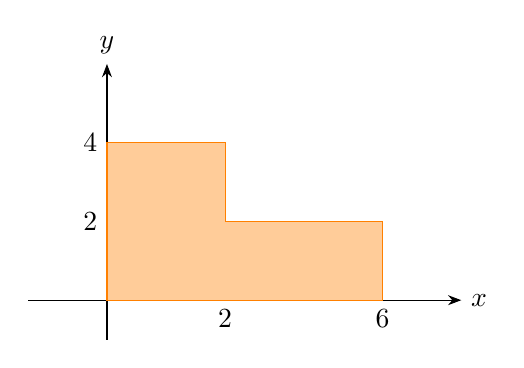
\begin{tikzpicture}[=>stealth]
\draw[-Stealth](-1,0)--(4.5,0)node[right]{$x$};
\draw[-Stealth](0,-0.5)--(0,3)node[above]{$y$};
\draw[orange](0,2)--(1.5,2)--(1.5,1)--(3.5,1)--(3.5,0)--(0,0)--cycle;
\draw(1.5,0)node[below]{$2$}
(3.5,0)node[below]{6}
(0,1)node[left]{2}
(0,2)node[left]{4};
\path[fill=orange,opacity=0.4](0,2)--(1.5,2)--(1.5,1)--(3.5,1)--(3.5,0)--(0,0)--cycle;
\end{tikzpicture}
\end{figure}

















Let $\hspace{0.2cm} w = az + b\hspace{0.2cm}$ with $\hspace{0.2cm} a = \dfrac{1 + i}{\sqrt{2}}\hspace{0.2cm}$ and $\hspace{0.2cm} b = 1 + 2i$\\ Sketch the image of $D$ in the $uv-$plane under the mapping $w = az + b$.\\



\textcolor{red}{Solution}\\

$\left|a\right| = \left|\dfrac{1 + i}{\sqrt{2}}\right| = 1$, so there is no change in size of $D$.\\

$Arg(a) = \dfrac{\pi}{4}$. So the region $D$ is rotated by an amount $\dfrac{\pi}{4}$ clockwise.\\


% DIAGRAM 3



\begin{figure}[H]
\centering
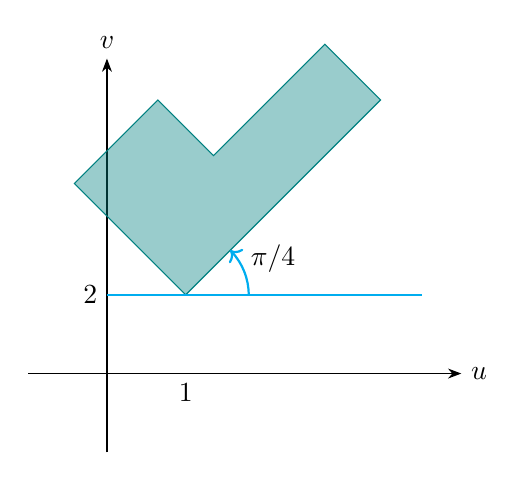
\begin{tikzpicture}[=>stealth]
\draw[-Stealth](-2,-1)--(3.5,-1)node[right]{$u$};
\draw[-Stealth](-1,-2)--(-1,3)node[above]{$v$};
\draw[teal,rotate=45](0,2)--(1.5,2)--(1.5,1)--(3.5,1)--(3.5,0)--(0,0)--cycle;
\draw(0,-1)node[below]{$1$}
(-1,0)node[left]{2};
\path[fill=teal,opacity=0.4,rotate=45](0,2)--(1.5,2)--(1.5,1)--(3.5,1)--(3.5,0)--(0,0)--cycle;
\coordinate (a) at (0.5,0);
\coordinate (b) at (0,0);
\coordinate (c) at (0.5,0.5);
\draw
pic[thick,draw=cyan, angle radius =0.8cm,->,angle eccentricity=1.5,"$\pi/4$"]{angle = a--b--c};
\draw[thick,cyan](-1,0)--(3,0);
\end{tikzpicture}
\end{figure}
















\textbf{\textcolor{red}{Example}}\\
Find the image of the region $\hspace{0.2cm} y> 1\hspace{0.2cm}$ under the transformation $\hspace{0.2cm}  w = (1 - i)z$.\\

\textcolor{red}{Solution}\\
Write $\hspace{0.2cm} w = (1 - i)z\hspace{0.2cm}$ in the form $\hspace{0.2cm} z = \dfrac{1}{2}(1 + i)w$, i.e make $z$ the subject.\\

Let $w = u + iv$ and $z = x + iy$. Then 

$$\boxed{x + iy = \dfrac{1}{2} (1 + i) (u + iv)}$$
So that $\hspace{0.2cm} x = \dfrac{u - v}{2}\hspace{0.2cm}$ and $\hspace{0.2cm} y = \dfrac{u + v}{2}$, so that the region $y > 1$ is transformed into the region $u + v>2$. in the $w-$plane.\\
When we move on the boundary line $y = 1$ from $i$ to $1 + i$, the region remains left to the observer.


% DIAGRAM 4


\begin{figure}[H]
\centering
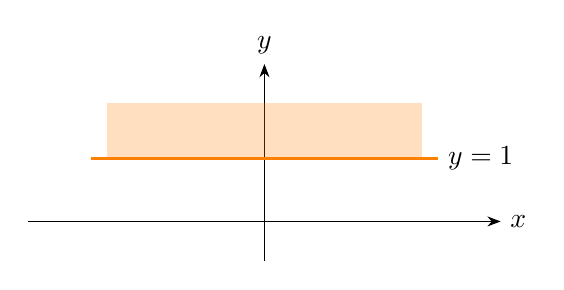
\begin{tikzpicture}[=>stealth]
\draw[-Stealth](-3,0)--(3,0)node[right]{$x$};
\draw[-Stealth](0,-0.5)--(0,2)node[above]{$y$};
\path[fill=orange,opacity=0.25](-2,0.8)--(-2,1.5)--(2,1.5)--(2,0.8)--cycle;
\draw[thick,orange](-2.2,0.8)--(2.2,0.8)node[right,black]{$y=1$};
\end{tikzpicture}
\end{figure}














This cases movement on the image line $u + v = 2$ from $w = 1 + i$ to $w = 2$, and hence the image region is taken left to the observer.


% DIAGRAM 5

\begin{figure}[H]
\centering
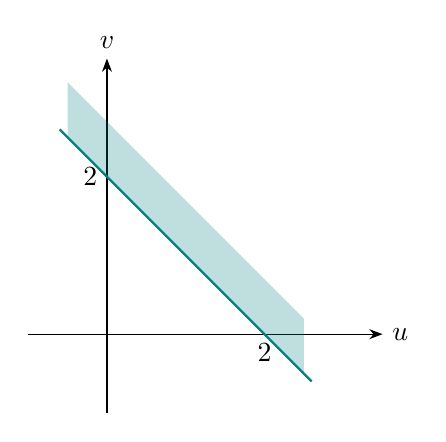
\begin{tikzpicture}[=>stealth]
\draw[-Stealth](-1,0)--(3.5,0)node[right]{$u$};
\draw[-Stealth](0,-1)--(0,3.5)node[above]{$v$};
\draw(0,2)node[left]{2}
(2,0)node[below]{2};
\path[fill=teal,opacity=0.25](-0.5,2.5)--(2.5,-0.5)--(2.5,0.2)--(-0.5,3.2)--cycle;
\draw[thick,teal](-0.6,2.6)--(2.6,-0.6);
\end{tikzpicture}
\end{figure}
















\textbf{\textcolor{red}{Example}}\\
Find the image of the semi-infinite strip $x> 0$, $\hspace{0.2cm} 1 < y < 2$ under the mapping $\hspace{0.2cm} w = iz + 1$.\\

\textcolor{red}{Solution}

% DIAGRAM 6


\begin{figure}[H]
\centering
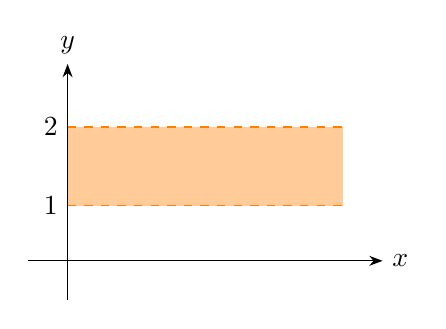
\begin{tikzpicture}[=>stealth]
\draw[-Stealth](-0.5,0)--(4,0)node[right]{$x$};
\draw[-Stealth](0,-0.5)--(0,2.5)node[above]{$y$};
\path[fill=orange,opacity=0.4](0,0.7)--(3.5,0.7)--(3.5,1.7)--(0,1.7)--cycle;
\draw[orange,dashed]
(0,0.7)--(3.5,0.7)
(0,1.7)--(3.5,1.7);
\draw(0,0.7)node[left]{1}
(0,1.7)node[left]{2};
\end{tikzpicture}
\end{figure}















We have $w = u + iv$ and $z = x + iy$, so that $\hspace{0.2cm} w =  i z + 1 \implies u + iv = i(x + iy) + 1\hspace{0.2cm}$ so that 
$$\boxed{u = 1 - y \hspace{0.2cm}\text{and}\hspace{0.2cm} v = x}$$
Now $\hspace{0.2cm} v = x  \implies v > 0\hspace{0.2cm}$ since $\hspace{0.2cm} x> 0$\\

$ 1 < y < 2 \implies 1 < 1 - u < 2$\\

$\implies \hspace{0.2cm} -1 < u < 0$\\
So the  image in the $uv-$plane is the strip $\hspace{0.2cm} v> 0, \hspace{0.2cm} - 1 < u < 0$



% DIAGRAM 7

\begin{figure}[H]
\centering
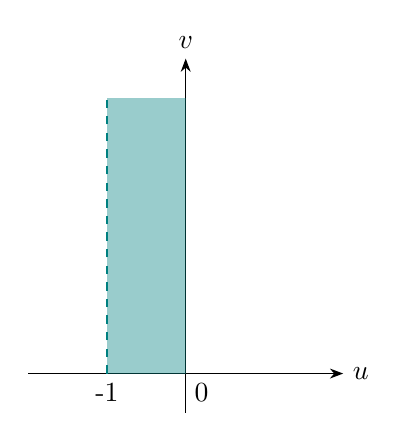
\begin{tikzpicture}[=>stealth]
\draw[-Stealth](-2,0)--(2,0)node[right]{$u$};
\draw[-Stealth](0,-0.5)--(0,4)node[above]{$v$};
\path[fill=teal,opacity=0.4](0,0)--(0,3.5)--(-1,3.5)--(-1,0)--cycle;
\draw(-1,0)node[below]{-1}
(0.2,0)node[below]{0};
\draw[dashed,teal](-1,0)--(-1,3.5);
\end{tikzpicture}
\end{figure}














\textbf{\textcolor{red}{Example}}\\
construct a linear transformation which 
\begin{enumerate}
\item Contains $\hspace{0.2cm} i\hspace{0.2cm}$ onto $\hspace{0.2cm} -i\hspace{0.2cm}$ and $\hspace{0.2cm} 1 + 2i\hspace{0.2cm}$ onto itself.
\item Maps $\hspace{0.2cm} \left|z - 1\right|  = 1\hspace{0.2cm}$ onto $\hspace{0.2cm} \left|w - 3i\right|= 2$\\
\end{enumerate}


\textcolor{red}{Solution}
\begin{enumerate}
\item $\hspace{0.2cm} w =  az + b\hspace{0.2cm}$ Replacing we have 
$$
\left.\begin{aligned}
-i & = a i + b\\
1 + 2i & = a(1 + 2i) + b\\
\end{aligned}
\right\} \hspace{0.2cm}\text{solve for} \hspace{0.2cm} a \hspace{0.2cm}\text{and}\hspace{0.2cm}b
$$
Doing that we get $\hspace{0.2cm} w = (2 + i)z + 1 - 3i$.\\


\item $\hspace{0.2cm} w = az + b$\\

$\left|z - 1\right| = 1\hspace{0.3cm}\longmapsto\hspace{0.3cm} \left|w - 3i\right| = 2$\\

$ w - 3i = 2(z - 1)$\\

$\implies\hspace{0.3cm} w = 2z - 2 + 3i$\\\\\\




\textcolor{blue}{Exercise}\\
$\left|z - 1\right| = 7 \hspace{0.4cm} \longmapsto \hspace{0.4cm}\left|w - 3i\right| = 2$\\

$w - 3i = \dfrac{2}{7} (z - 1)$\\\\
\end{enumerate}








\textbf{\textcolor{blue}{Exercise}}
\begin{enumerate}
\item Given a triangle $\triangle$ in the $z$ plane with vertices $\hspace{0.2cm} i, \hspace{0.2cm} 1 - i, \hspace{0.2cm} 1 + i\hspace{0.2cm}$ determine the triangle $\triangle'$ onto which $\triangle$ is mapped under the transformation
\begin{enumerate}
    \item $\hspace{0.2cm} w = 3z + 4 - 2i$
    \item $\hspace{0.2cm} w = iz + 2 - i$. What is the relation between $\triangle$ and $\triangle'$ in each case?
\end{enumerate}

\item Find the linear transformation that maps the imaginary axis onto the line with points $\hspace{0.2cm} i\hspace{0.2cm}$ and $\hspace{0.2cm} 1 + 2i$.\\
\end{enumerate}




{\color[wave]{485}\subsection{The Identity Mapping}}
If we set $a = 1$ and $b = 0$ in $\hspace{0.2cm} w = az + b, \hspace{0.2cm}$ we obtain the identity  mapping $\hspace{0.2cm} w = z$.\\
This mapping simply reproduces in the $w-$plane the exact copy of the region in the $z-$plane.\\\\\\






{\color[wave]{485}\subsection{The Mapping $w = z^c$}}
Setting $\hspace{0.2cm} w = \rho e^{i\phi}\hspace{0.2cm}$ and $\hspace{0.2cm} z =re^{i\theta}\hspace{0.2cm}$ we get, for $c$ real and $+ve$, 
\begin{align*}
\rho & = \left|w\right| = r^c \hspace{0.3cm} \text{and}\\\\
\phi & = c \hspace{0.1cm} Arg(z) + 2k\pi\\
& = c\theta + 2k\pi\hspace{0.1cm},\hspace{0.2cm} k\in \mathbb{Z}\hspace{0.1cm}, \hspace{0.2cm} \text{under the mapping}\hspace{0.2cm} w = z^c
\end{align*}


This shows that when $c\neq 1$, a non-uniform scale factor $ r^c$ is involved in the mapping, with magnification when $r> 1$ and contraction when $r < 1$.\\

The ray $\hspace{0.2cm} r> 0, \hspace{0.2cm} \theta  = \theta_0\hspace{0.2cm}$ in the $z-$plane is mapped onto the ray $\hspace{0.2cm} \rho = r^c\hspace{0.2cm}, \hspace{0.2cm} \phi = \phi_0 = c\theta_0\hspace{0.2cm}$ in the $w-$plane.\\
The function $\hspace{0.2cm} w = z^c\hspace{0.2cm}$ with this gives valued function of the $z-$plane onto the $w-$plane for $ c  > 1$, unless $\theta $ is suitably restricted.\\

Consider, for simplicity, $c = 2$. The mapping $\hspace{0.2cm} w = z^c\hspace{0.2cm}$ will then be $$\boxed{\rho e^{i\pi} = r^2 e^{2i\theta}}$$
The image of the point $(r, \theta)$ in the $z-$plane is that point in $w-$plane with polar coordinates $\hspace{0.2cm} (\rho, \phi) = (r^2, 2\theta)$.\\

This shows that the first quadrant of the $z-$plane is mapped onto the entire upper half plane. For, first quadrant is $\hspace{0.2cm} 0 \leq \theta \leq \dfrac{\pi}{2}, \hspace{0.2cm} r> 0\hspace{0.2cm}$ and the upper half plane is defined by\\ $\hspace{0.2cm} 0 \leq \dfrac{\phi}{2}\leq \dfrac{\pi}{2}\hspace{0.2cm}, \hspace{0.2cm} \rho = r^2 $  $$\implies \hspace{0.4cm} 0 \leq \phi \leq \pi\hspace{0.2cm}, \hspace{0.3cm} \rho = r^2 > 0$$

circles about the origin, $r = r_0$ are transformed into circles $\rho = r^2$ in the $w-$plane.\\


The semicircular region $r = r_0, \hspace{0.2cm} 0\leq \theta \leq \pi\hspace{0.2cm}$ is mapped into the circular region $\hspace{0.2cm} \phi = r^2_0$.\\

In Cartesian form, set $\hspace{0.2cm} w = u + iv\hspace{0.2cm}$ and $\hspace{0.2cm} w = z^2,\hspace{0.2cm} $ we have $\hspace{0.2cm} u = x^2 - y^2\hspace{0.2cm} , \hspace{0.2cm} v = 2xy$\\

Hence the hyperbolas $\hspace{0.2cm} x^2 - y^2 = c$ and $\hspace{0.2cm} 2xy = d\hspace{0.2cm}$ are mapped by $\hspace{0.2cm} w = z^2\hspace{0.2cm}$ into straight line $\hspace{0.2cm} u = c \hspace{0.2cm}$ and $\hspace{0.2cm} v = d$.\\

One fact is that when $c$ and $d$ are not zero, the hyperbolas intersect at right angles, just their images.\\\\\\





\textbf{\textcolor{red}{Example}}\\
Find the image of the vertical strip $\hspace{0.2cm} 0\leq x \leq c\hspace{0.2cm}, \hspace{0.2cm} y\leq 0\hspace{0.2cm}$ under the map $\hspace{0.2cm} w = z^2$.\\\\

\textcolor{red}{Solution}\\
Let $\hspace{0.2cm} x = \alpha \hspace{0.2cm}, \hspace{0.2cm} 0 < \alpha < c\hspace{0.2cm}$ be a line in the region and let $(\alpha ,y)$ be a movable point on the line $\hspace{0.2cm} x = \alpha $.\\
The image of this point is given by the relations $\hspace{0.2cm} u  = \alpha^2 - y^2\hspace{0.2cm}, \hspace{0.2cm} v = 2\alpha y \hspace{0.2cm}, \hspace{0.2cm} y\leq 0$.\\

Eliminating $\hspace{0.2cm} y$ , get $\hspace{0.2cm} v^2= -4\alpha^2 (u- \alpha^2)$.\\

This is an equation of a parabola, vertex at $(\alpha^2, 0)$ and focus at the origin.\\
Since $v$ increases as $y$ increases, the point $(\alpha , y)$ moves upwards on the line $ x = \alpha$ and the image point moves left on the curve $A'$.\\

The image of $x = c$ is the curve $c$.



% DIAGRAM 11

\begin{figure}[H]
\centering
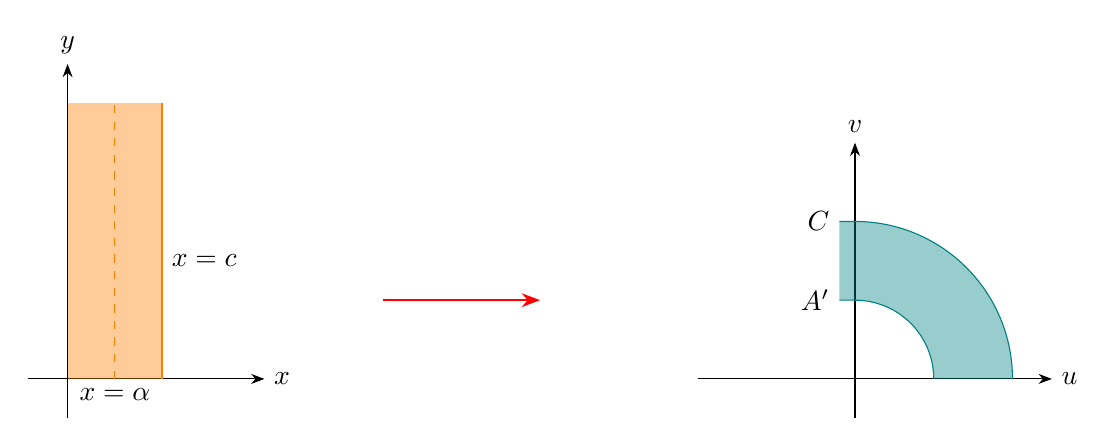
\begin{tikzpicture}[=>stealth]
\draw[-Stealth](-0.5,0)--(2.5,0)node[right]{$x$};
\draw[-Stealth](0,-0.5)--(0,4)node[above]{$y$};
\draw(0.6,0)node[below]{$x=\alpha$}
(1.2,1.5)node[right]{$x=c$};
\draw[thick,orange](1.2,0)--(1.2,3.5);
\draw[dashed,orange](0.6,0)--(0.6,3.5);
\path[fill=orange,opacity=0.4](0,0)--(1.2,0)--(1.2,3.5)--(0,3.5)--cycle;
\draw[thick,red,-Stealth](4,1)--(6,1);
\draw[-Stealth](8,0)--(12.5,0)node[right]{$u$};
\draw[-Stealth](10,-0.5)--(10,3)node[above]{$v$};
\draw[teal]
(12,0)arc[start angle = 0, end angle =90,radius=2cm]--(9.8,2)
(11,0)arc[start angle =0,end angle=90,radius=1cm]--(9.8,1);
\path[fill=teal,opacity=0.4](12,0)arc[start angle = 0, end angle =90,radius=2cm]--(9.8,2)--(9.8,1)--(10,1)arc[start angle =90,end angle=0,radius=1cm]--(11,0)--(12,0)--cycle;
\draw(9.8,2)node[left]{$C$}
(9.8,1)node[left]{$A'$};
\end{tikzpicture}
\end{figure}
















Further, the image of the line $x = 0$, $\hspace{0.2cm} y \leq 0$ of the region is found to be $u = -y^2\hspace{0.2cm},\hspace{0.2cm} v = 0$.\\
This means that the negative real axis, the image of the positive $y-$axis in the $z-$plane.\\\\




\textbf{\textcolor{red}{Example}}\\
Show that the image of the closed triangular region formed by the lines $\hspace{0.2cm} y = \pm x\hspace{0.2cm}$ and $\hspace{0.2cm} x = 1\hspace{0.2cm}$ is the closed parabolic region bounded by the segment $\hspace{0.2cm} -2\leq v \leq 2\hspace{0.2cm}$ of the $v-$axis on the right portion of a parabola $\hspace{0.2cm} v^2 = -4(u - 1)\hspace{0.2cm}$ under the map $\hspace{0.2cm} w = z^2$.\\


\textcolor{red}{Solution}\\
We have $\hspace{0.2cm} u = x^2 -y^2,\hspace{0.3cm} v = 2xy$

\begin{enumerate}
\item The line $\hspace{0.2cm} y = x\hspace{0.2cm} , \hspace{0.2cm} 0 \leq y \leq 1\hspace{0.2cm}$ is mapped on $ u = 0$ and $v = 2y^2$ and the point $(1,1)$ is mapped onto $(0,2)$.
\item The line $\hspace{0.2cm} y = -x\hspace{0.2cm} , \hspace{0.2cm} -1\leq y \leq 0\hspace{0.2cm}$ is mapped onto $\hspace{0.2cm} u = 0, \hspace{0.2cm} v = -2y^2\hspace{0.2cm}$ and the point $(1,-1)$ is mapped to $(0,-2)$.
\item The line $\hspace{0.2cm} x = 1\hspace{0.2cm}$ is mapped on $\hspace{0.2cm} v^2 = -4(u - 1)\hspace{0.2cm}$ a parabola with vertex  $(1,0)$ and focus at the origin. The parabola meets the line $u = 0$ at $(0,2)$ and $(0,-2)$.



% DIAGRAM 12



\begin{figure}[H]
\centering
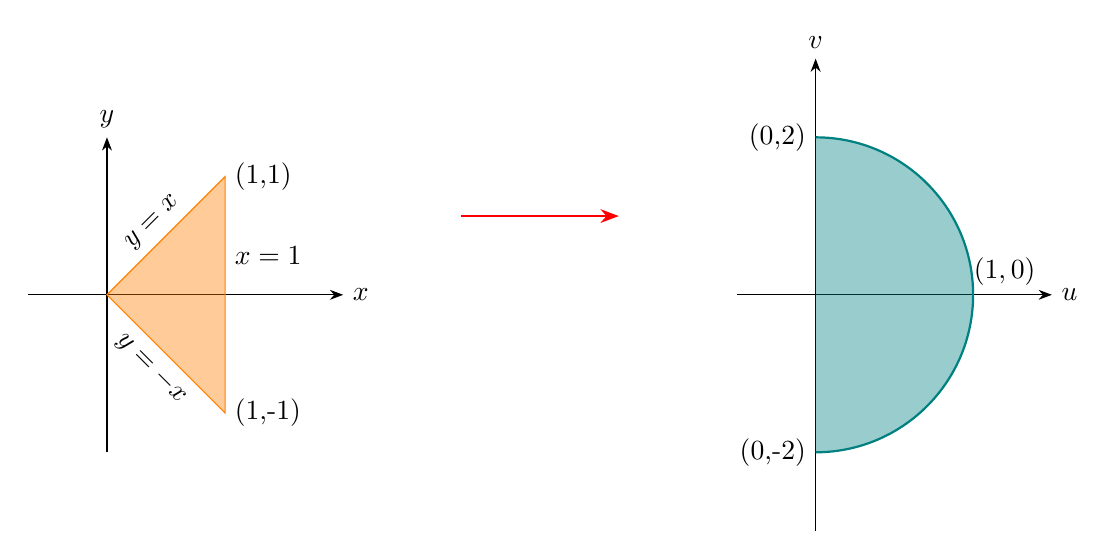
\begin{tikzpicture}[=>stealth]
\draw[-Stealth](-1,0)--(3,0)node[right]{$x$};
\draw[-Stealth](0,-2)--(0,2)node[above]{$y$};
\draw[orange](0,0)--node[sloped,above,black]{$y =x$}(1.5,1.5)--(1.5,-1.5)--node[sloped,below,black]{$y=-x$}cycle;
\draw(1.5,1.5)node[right]{(1,1)}
(1.5,-1.5)node[right]{(1,-1)}
(1.5,0.5)node[right]{$x=1$};
\path[fill=orange,opacity=0.4](0,0)--(1.5,1.5)--(1.5,-1.5)--cycle;
\draw[thick,-Stealth,red](4.5,1)--(6.5,1);
\draw[-Stealth](8,0)--(12,0)node[right]{$u$};
\draw[-Stealth](9,-3)--(9,3)node[above]{$v$};
\draw[thick,teal](9,-2)arc[start angle=270, end angle=450, radius = 2cm];
\path[fill=teal,opacity=0.4](9,-2)arc[start angle=270, end angle=450, radius = 2cm];
\draw(9,2)node[left]{(0,2)}
(9,-2)node[left]{(0,-2)}
(11.4,0)node[above]{$(1,0)$};
\end{tikzpicture}
\end{figure}




\end{enumerate}






\textbf{\textcolor{teal}{Exercise}}\\
Find the  image of the given set under the mapping $\hspace{0.2cm} w = z^2\hspace{0.2cm}$. Draw the set and its image in there respective planes
\begin{enumerate}
\item $\hspace{0.2cm} arg z = \dfrac{\pi}{3}$

\item $\hspace{0.2cm} arg z = \dfrac{-3\pi}{4}$

\item $\hspace{0.2cm} y = -\dfrac{1}{4}$

\item $\hspace{0.2cm} x  = 0 \hspace{0.2cm}, \hspace{0.2cm} y > 0$

\item $\hspace{0.2cm} $ the circular arc $\left|z\right| = \dfrac{4}{3}$

\item $\hspace{0.2cm}$ The triangle with vertices 0 , $\hspace{0.2cm} 1 + 2i\hspace{0.2cm}$ and $\hspace{0.2cm} -1 + 2i$.

\item $\hspace{0.2cm}$ The triangular region bounded by $\hspace{0.2cm}  x = 1, \hspace{0.2cm} y = 1\hspace{0.2cm}$ and $\hspace{0.2cm} x  + y = 1$

\item $\hspace{0.2cm} 1\leq \left|z\right|\leq 2\hspace{0.3cm},\hspace{0.3cm} \dfrac{\pi}{4}\leq \operatorname{arg}(z)\leq \dfrac{3\pi}{4}$\\\\\\
\end{enumerate}





{\color[wave]{485}\subsection{The Mapping $w = z^{1/2}$}}
If we square both sides of $\hspace{0.2cm} w = z^{1/2}\hspace{0.2cm}$ get $\hspace{0.2cm} w^2 = z.\hspace{0.2cm}$ Setting $\hspace{0.2cm} w = u + iv\hspace{0.2cm}, \hspace{0.2cm}  z = x+ iy,\hspace{0.2cm}$  we get $$\boxed{x = u^2 - v^2 \hspace{0.4cm}\text{and}\hspace{0.4cm} y = 2uv}$$
This shows that the line $\hspace{0.2cm} x = a\hspace{0.2cm} (a> 0)\hspace{0.2cm}$ in the $z-$plane gets mapped to the parabola $\hspace{0.2cm} u^2 - v^2 = a\hspace{0.2cm}, \hspace{0.2cm}$ while the line $\hspace{0.2cm} y = b\hspace{0.2cm} (b> 0)\hspace{0.2cm}$ is mapped to the parabola $\hspace{0.2cm} b = 2uv$.\\\\\\





\pagebreak
{\color[wave]{485}\subsection{The Inversion Mapping $w = \dfrac{1}{z}$}}
In polar form if $\hspace{0.2cm} z = re^{i\theta}\hspace{0.2cm}$ and $ \hspace{0.2cm} w = \rho e^{i\phi}\hspace{0.2cm}$ then we have $$\boxed{\rho e^{i\phi}  = \dfrac{1}{r}e^{-i\theta}}$$
So that $\hspace{0.2cm}\rho = \dfrac{1}{r}\hspace{0.2cm}$ and $\hspace{0.2cm} \phi = -\theta.\hspace{0.2cm}$ Since the radius under goes an inversion, the mapping $\hspace{0.2cm} w = \dfrac{1}{z}\hspace{0.2cm}$ is called an inversion mapping.\\
There is a one-one correspondence between points in the $z-$plane and points in the $w-$plane, except the points $\hspace{0.2cm} z = 0\hspace{0.2cm}$ and $\hspace{0.2cm} w = 0\hspace{0.2cm}$ which have no images.


% DIAGRAM 13


\begin{figure}[H]
\centering
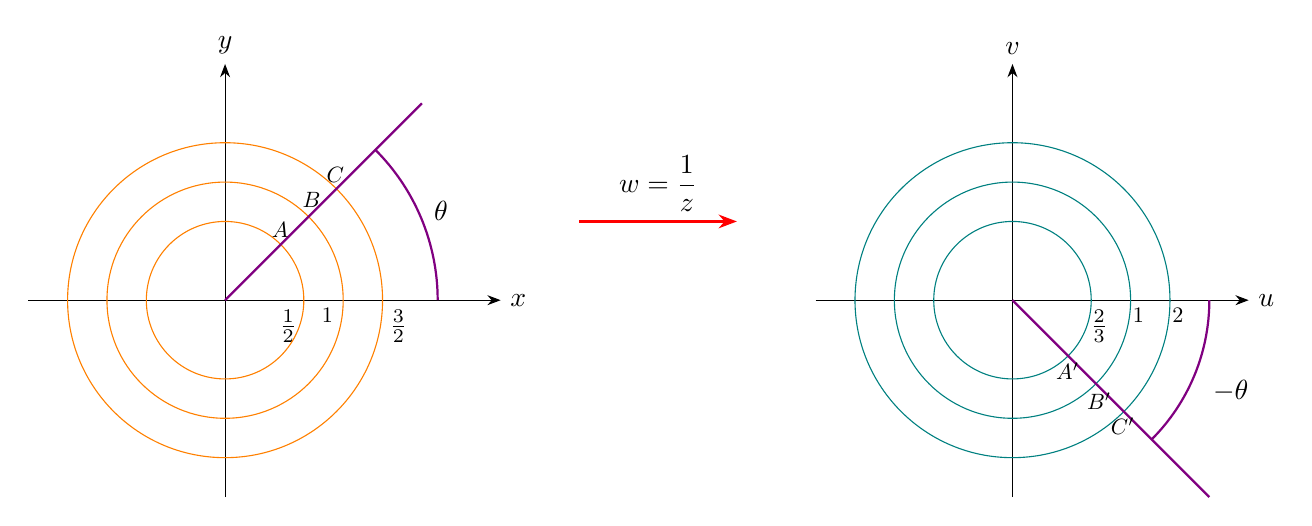
\begin{tikzpicture}[=>stealth]
\draw[-Stealth](-2.5,0)--(3.5,0)node[right]{$x$};
\draw[-Stealth](0,-2.5)--(0,3)node[above]{$y$};
\draw(0.8,0)node[below]{$\frac{1}{2}$}
(1.3,0)node[below,scale=0.8]{$1$}
(2.2,0)node[below]{$\frac{3}{2}$};
\draw[orange]
(0,0)circle[radius=1cm]
(0,0)circle[radius=1.5cm]
(0,0)circle[radius=2cm];
\draw[thick,violet](0,0)--(2.5,2.5);
\coordinate (a) at (0.5,0);
\coordinate (b) at (0,0);
\coordinate (c) at (0.5,0.5);
\draw
pic[thick, draw=violet,-, angle radius =2.7cm, angle eccentricity=1.1,"$\theta$"]{angle = a--b--c};
\draw(0.7,0.7)node[above,scale=0.8]{$A$}
(1.1,1.08)node[above,scale=0.8]{$B$}
(1.4,1.4)node[above,scale=0.8]{$C$}
(5.5,1)node[above]{$w=\dfrac{1}{z}$};
\draw[thick,red,-Stealth](4.5,1)--(6.5,1);
\draw[-Stealth](7.5,0)--(13,0)node[right]{$u$};
\draw[-Stealth](10,-2.5)--(10,3)node[above]{$v$};
\draw[teal]
(10,0)circle[radius=1cm]
(10,0)circle[radius=1.5cm]
(10,0)circle[radius=2cm];
\draw(11.1,0)node[below]{$\frac{2}{3}$}
(11.6,0)node[below,scale=0.8]{$1$}
(12.1,0)node[below,scale=0.8]{2};
\draw[thick,violet](10,0)--(12.5,-2.5);
\draw(10.7,-0.7)node[below,scale=0.8]{$A'$}
(11.1,-1.08)node[below,scale=0.8]{$B'$}
(11.4,-1.4)node[below,scale=0.8]{$C'$};
\coordinate (A) at (10.5,0);
\coordinate (B) at (10,0);
\coordinate (C) at (10.5,-0.5);
\draw
pic[thick,draw=violet,angle radius=2.5cm,angle eccentricity=1.2,"$-\theta$"]{angle=C--B--A};
\end{tikzpicture}
\end{figure}
















The inversion mapping $\hspace{0.2cm} w = \dfrac{1}{z}\hspace{0.2cm}$ sends circles centered at the origin in $z-$plane into circles centered at the origin in the $w-$plane.\\
In general, the mapping $\hspace{0.2cm} w = \dfrac{1}{z}\hspace{0.2cm}$ sends circles into circles or straight lines.\\

Consider any circle
\begin{equation}
\boxed{(x-a)^2 + (y - b)^2 = c^2}
\end{equation}


In the $z-$plane centered at $(a,b)$ with radius $c$. Setting $\hspace{0.2cm} x = \dfrac{z + \overline{z}}{2}\hspace{0.2cm}$ and $\hspace{0.2cm} y = \dfrac{z - \overline{z}}{2i}\hspace{0.1cm}, \hspace{0.2cm}$ then $(1)$ becomes
\begin{equation}
\boxed{z\overline{z} + Az + \overline{Az} + B  = 0}\\
\end{equation}



From $\hspace{0.2cm} w = \dfrac{1}{z}\hspace{0.1cm}, \hspace{0.2cm}$ get $\hspace{0.2cm} z = \dfrac{1}{w}\hspace{0.2cm}$ and $\hspace{0.2cm} \overline{z} = \dfrac{1}{\overline{w}}$.\\

So that the image in the $w-$plane or the circle $(2)$ is 
\begin{equation}
\boxed{\dfrac{1}{w\overline{w}} + \dfrac{A}{w} + \dfrac{\overline{A}}{\overline{w}} + B = 0}\\
\end{equation}



At this we consider two cases $\hspace{0.2cm} B\neq 0\hspace{0.2cm}$ and $\hspace{0.2cm} B = 0;\hspace{0.2cm} B = 0\hspace{0.2cm}$ corresponds the case when the circle $(1)$  passes through the origin and $\hspace{0.2cm} B\neq 0\hspace{0.2cm}$, case where circle in $z-$plane does not pass the origin.\\

\begin{enumerate}
\item $B\neq 0\hspace{0.2cm}$ (circles not through $z = 0$)\\
If $B \neq 0$, we can write (3) as 
$\hspace{0.2cm}\boxed{w\overline{w} + \dfrac{\overline{A}}{B}w + \dfrac{A}{B}\overline{w} + \dfrac{1}{B} = 0}, \hspace{0.2cm}$ which is of the same form as (2) since $\hspace{0.2cm} \dfrac{1}{B}\hspace{0.2cm}$ is real, and take coefficient $\hspace{0.2cm}\dfrac{A}{B}\hspace{0.2cm}$ is  the complex conjugate of $\hspace{0.2cm}\dfrac{\overline{A}}{B}.\hspace{0.2cm}$ Thus the image is a circle.


\item $B = 0$ (circles through $ z = 0$)\\
If $B = 0$, we can write (3) as $\hspace{0.2cm} 1 + A\overline{w} + \overline{A}w = 0,\hspace{0.2cm}$ in terms of $u$ and $v$ as $$bv - au + \dfrac{1}{2} = 0$$ which is a straight line.\\
\end{enumerate}



One can show that $\hspace{0.2cm} w = \dfrac{1}{z}\hspace{0.2cm}$ sends straight lines that do not pass through the origin into circles and straight lines through $z = 0$ into straight lines.\\

Check by considering $\hspace{0.2cm}ax + by + c = 0\hspace{0.2cm} $ in the $z-$plane. $\hspace{0.2cm} u + iv = \dfrac{1}{x + iy}$.\\\\\\












{\color[wave]{485}\subsection{The Point at Infinity}}
Under the mapping $\hspace{0.2cm}  w = \dfrac{1}{z}\hspace{0.2cm}$ or $\hspace{0.2cm} \rho e^{i\phi} = \dfrac{1}{r}e^{-i\theta},\hspace{0.2cm}$ the points $z$ interior to the circle $\hspace{0.2cm} r = R\hspace{0.2cm}$ map into points $w$ interior to the circle $\hspace{0.2cm} \rho = \dfrac{1}{R}$.\\

The point $\hspace{0.2cm} w = 0\hspace{0.2cm}$ is not an image.\\

By making $R$ large enough all points $z$ outside the large circle fall within an arbitrary small neighbourhood of $\hspace{0.2cm} w = 0$\\

We can take of talk of the points of infinity, i.e $\hspace{0.2cm} w = \infty.$\\

This is the image of $\hspace{0.2cm} z = 0\hspace{0.2cm}$ in the $z-$plane.\\\\




\textbf{\textcolor{red}{Example}}\\
The function $\hspace{0.2cm} w =\dfrac{4z^2}{(1 - z)^2}\hspace{0.2cm}$ maps the point $\hspace{0.2cm} z = \infty\hspace{0.2cm}$ into the point $\hspace{0.2cm} w = 4$ in the $w-$plane.\\

For, if we write $\hspace{0.2cm} z = \dfrac{1}{z'},\hspace{0.2cm}$ so that $$ w = \dfrac{\dfrac{4}{z'^2}}{\Big(1 - \dfrac{1}{z'}\Big)^2} = \dfrac{4}{(z' - 1)^2}$$
Setting $\hspace{0.2cm} z' = 0 \hspace{0.2cm} (z =\infty)\hspace{0.2cm}$ get $w = 4$.\\\\

One checks that $\hspace{0.2cm} w = \infty\hspace{0.2cm}$ is the image of the point $z = 1$ in the $z-$plane. $\hspace{0.3cm} \Big($ set $w = \dfrac{1}{w'}\Big)$.\\\\\\








 






{\color[wave]{485}\subsection{Fixed Points}}
A fixed point of $\hspace{0.2cm} w = f(z)\hspace{0.2cm}$ is a point $z_0$ such that $\hspace{0.2cm} z_0 = f(z_0)$.\\

If $\hspace{0.2cm} w = az + b,\hspace{0.2cm}$ the fixed points are determined by $\hspace{0.2cm} z_0 = az_0 + b \hspace{0.2cm}$ or $\hspace{0.2cm} z_0 = \dfrac{b}{ 1 - a}\hspace{0.2cm}$ for $\hspace{0.2cm} a\neq 1$.\\

So for $a\neq 1$, $\hspace{0.2cm} w = az + b\hspace{0.2cm}$ has a finite fixed point $\hspace{0.2cm} z_0 = \dfrac{b}{1 - a}$.\\

If $a = 1,\hspace{0.2cm} w = z + b\hspace{0.2cm}$ has no fixed points in $\mathbb{C}$.\\

We can then extended $\mathbb{C}$ to $\hspace{0.2cm} \overline{\mathbb{C}} = \mathbb{C}\cup \{\pm \infty\}.\hspace{0.2cm}$ Thus in the extended plane, the point at infinity $\hspace{0.2cm} w = \infty\hspace{0.2cm}$ is a fixed point of the translation $\hspace{0.2cm} w = z + b$.\\\\\\





\textbf{\textcolor{teal}{Exercise}}\\
Find the fixed points of the identity map and the inversion mapping.\\\\\\






{\color[wave]{485}\subsection{Paths and Smooth Paths}}
A path in a region $G\subset \mathbb{C}$ is a continuous function $\hspace{0.2cm} \gamma : [a,b] \longrightarrow G\hspace{0.2cm}$ for some interval $[a,b]$ in $\mathbb{R}$.\\

If $\gamma'(t)$ exists for each $t\in [a,b]$ and $\gamma'(t): [a,b]\longrightarrow \mathbb{C}$ is continuous, we say that $\gamma$ is a smooth path.\\

Also $\gamma$ is said to be piece wise smooth if there is a partition of $[a,b]$, say\\ $\hspace{0.2cm} a = t_0 < t_1< \cdots\cdots\cdots < t_n = b$ such that $\gamma$ is smooth one each sub interval of $[t_{i-1},ti]$.\\

Suppose that $\hspace{0.2cm} \gamma: [a,b] \longrightarrow G\hspace{0.2cm}$ is a differentiable path(smooth) and that for some\\ $t_0 \in (a,b),\hspace{0.2cm} \gamma'(t_0) \neq 0$.\\

Then $\gamma$ has a tangent at the point $\gamma (t_0)$. The slope of the tangent line is $\tan (arg\gamma'(t_0))$.


% DIAGRAM 14 

\begin{figure}[H]
\centering
\begin{tikzpicture}[=>stealth]
\draw[thick,cyan,rotate=45](0,0)parabola(2,2)
(0,0)parabola(-2,2)node[right,black]{$\gamma$};
\draw(0,0)node[shape=circle,draw=cyan,fill=cyan,scale=0.01cm]{};
\draw[red,thick](-2,-2)--(2,2);
\draw[dashed](0,0)--(0,-1)node[below]{$t_0$};
\draw[red](1,1)--node[above,black,sloped]{$\gamma'(t_0)$}(2,2);
\end{tikzpicture}
\end{figure}














If $\gamma_1$ and $\gamma_2$ are two paths with $\gamma_1(t_1) = \gamma_2 (t_2)  = z_0\hspace{0.2cm}$ (say) and $\hspace{0.2cm} \gamma'_1 (t_1) \neq 0 \neq \gamma'_2(t_2),\hspace{0.2cm}$ then we define the angle between $\gamma_1$ and $\gamma_2$ at $z_0$ to be 
$$\boxed{arg\gamma'_2(t_2) - arg\gamma'_1(t_1)}$$\\

% DIAGRAM 15

% Not clear


















Suppose $\gamma$ is a path in $G$ and $f: G \longmapsto \mathbb{C}$ is analytic. Then\\
$$\boxed{
\rho = fo\gamma\hspace{0.2cm} \text{is also a path and} \hspace{0.2cm} \rho'(t) = f'(\gamma(t))\cdot \gamma'(t)\hspace{0.2cm}\text{ by chain rule}}$$\\


Let $\hspace{0.2cm} z_0 = \gamma (t_0)\hspace{0.2cm}$ and suppose $\hspace{0.2cm} \gamma'(t_0) \neq 0\hspace{0.2cm}$ and $\hspace{0.2cm} f'(z_0) \neq 0,\hspace{0.2cm} \rho'(t_0) \neq 0$.

$$\boxed{arg \rho'(t_0) = argf'(z_0) + arg \gamma'(t_0)}$$\\


This gives $$arg \rho'(t_0) - arg \gamma'(t_0) = arg f'(z_0)\hspace{0.5cm}\cdots\cdots\cdots\cdots\hspace{0.4cm} (1)$$

Now let $\gamma_1$ and $\gamma_2$ be paths with  $\hspace{0.2cm} \gamma_1 (t_1) = \gamma_2(t_2) = z_0\hspace{0.2cm}$ and $\hspace{0.2cm} \gamma'_1(t_1) \neq  0 \neq \gamma'_2(t_2)$.\\

Let $\hspace{0.2cm} \rho_1 = fo\gamma_1\hspace{0.2cm}$ and $\hspace{0.2cm} \rho_2 = fo\gamma_2$.\\

Suppose also that the paths $\gamma_1$ and $\gamma_2$ are not tangents to each other at $z_0$. i.e $\hspace{0.2cm} \gamma'(t_1) \neq \gamma'(t_2)$.\\

From equation $(1)$ we get  $$arg \gamma'_2(t_2) - arg\gamma'_1(t_1) = arg \rho'_2(t_2) - arg \rho'_1(t_1)$$

Thus given any two paths through $z_0\hspace{0.2cm}f$ maps these paths onto two paths through $\hspace{0.2cm} w_0 = f(z_0)\hspace{0.2cm}$ and when $\hspace{0.2cm} f'(z_0) \neq 0,\hspace{0.2cm}$ the angles between the curves are preserved both in magnitude and direction. We have thus proved.\\\\




\textbf{\textcolor{teal}{Theorem}}\\
Let $\hspace{0.2cm} f: G \longmapsto \mathbb{C}\hspace{0.2cm}$ be analytic. Then $f$ preserves angles at each point $z_0$ of $G$ when $\hspace{0.2cm} f'(z_0) \neq 0.\hspace{0.2cm}$ In other words $f$ is a conformal mapping.\\\\




\textbf{\textcolor{teal}{Definition}}\\
Let $\hspace{0.2cm} f: G \longmapsto \mathbb{C}$ be such that which preserves angles and $\hspace{0.2cm} \lim\limits_{z \rightarrow z_0} \dfrac{\left|f(z) - f(z_0)\right|
}{\left|z - z_0\right|
}\hspace{0.2cm}$ exists, then $f$ is called a conformal mapping if $f$ is analytic and $\hspace{0.2cm} f'(z) \neq 0\hspace{0.2cm}$ for any $z$, then $f$ is conformal.\\


The converse is also true.\\\\



\textbf{\textcolor{red}{Example}}\\
The mapping $\hspace{0.2cm} w = f(z) = e^z\hspace{0.2cm}$ is conformal throughout $\mathbb{C}$.\\

$f(z)$ is analytic and $\hspace{0.2cm} f'(z) \neq 0\hspace{0.2cm}$ for all $z$. But $\hspace{0.2cm} z = c + iy\hspace{0.2cm}$ where $c$ is fixed then $\hspace{0.2cm} f(z) = re^{iy}\hspace{0.2cm}$ where $r = e^c$.\\

This shows that the map $\hspace{0.2cm} w = e^z\hspace{0.2cm}$ sends the straight line $\hspace{0.2cm} x = c\hspace{0.2cm}$ onto a circle with centre origin and radius $e^c$.\\

Also, $f$ maps the line $\hspace{0.2cm} y = d\hspace{0.2cm}$ onto the infinite ray $\hspace{0.3cm}\{re^{id}:\hspace{0.2cm} 0 < r< \infty\}$

$$y = d\iff z = x + id$$\\\\







\textbf{\textcolor{red}{Example}}\\
Verify by talking the curve $\hspace{0.2cm} y = x - 1$ $$\text{i.e}\hspace{0.2cm} z(x) = x + i(x -1)\hspace{0.2cm}, \hspace{0.2cm} -\infty < x < \infty$$ the angle of rotation under the transformation $\hspace{0.2cm} w = z^2\hspace{0.2cm}$ at the point $\hspace{0.2cm} 2 +i$.\\


\textcolor{red}{Solution}\\
By definition the angle of rotation for $\hspace{0.2cm} f(z) = z^2\hspace{0.2cm}$ at $\hspace{0.2cm} 2 + i\hspace{0.2cm}$ given by 
\begin{align*}
\operatorname{arg}( f'(2+i)) &  = \operatorname{arg} (4 + 2i)\\
& = \tan^{-1}\Big(\dfrac{1}{2}\Big) + 2n\pi
\end{align*}
The line $\hspace{0.2cm} y = x - 1\hspace{0.2cm}$ makes an angle $\hspace{0.2cm} \theta = \dfrac{\pi}{4}\hspace{0.2cm}$ with the $x-$axis.\\

The image of $\hspace{0.2cm} y = x - 1\hspace{0.2cm}$ under the map $\hspace{0.2cm} w = z^2\hspace{0.2cm}$ is given by using the relations. 
$$ u = x^2 - y^2 \hspace{0.3cm} \text{and}\hspace{0.4cm} v = 2xy$$ as $\hspace{0.2cm} v = \dfrac{u^2 - 1}{2}.\hspace{0.2cm}$ The image of $\hspace{0.2cm} 2 + i\hspace{0.2cm}$ is $\hspace{0.2cm} 3 + 4i\hspace{0.2cm}$ in the $w-$plane.\\

Now, for the image curve $\hspace{0.2cm} v = \dfrac{u^2 - 1}{2}$ $$ w = u +iv = u + i\Big(\dfrac{u^2 - 1}{2}\Big)$$
\begin{align*}
\phi & = arg \Bigg(w'\Bigg|_{w = 3 + 4i}\Bigg)\\\\
& = \operatorname{arg}( 1 +i4)\\
& = \operatorname{arg}( 1 + 3i)\\
& = \tan^{-1}(3)
\end{align*}

Thus the angle of rotation in $w-$plane is 
\begin{align*}
\phi - \theta & = \tan^{-1}(3) - \dfrac{\pi}{4}\\
& = \tan^{-1}(3) - \tan^{-1}(1)\\
& = \tan^{-1}\Big(\dfrac{3 - 1}{1 + 3}\Big)\\
& = \tan^{-1}\Big(\dfrac{1}{2}\Big)\\\\
\end{align*}







{\color[wave]{485}\subsection{Linear Fractional Transformations}}
Let $a, b,c$ and $d$ be any real or complex constants. Then the linear fractional transformation (LTF) $\hspace{0.2cm} w = T(z)\hspace{0.2cm}$ is defined to be the analytic function of the form 
$$\boxed {w = T(z) = \dfrac{az + b}{cz + d}\hspace{0.5cm} \cdots\cdots\cdots\hspace{0.5cm} (1)\hspace{0.5cm}\text{with}\hspace{0.3cm} ad - bc \neq 0}$$

This transformation is also called the Mobuis transformation or the Bi linear transformation. This transformation defines $w$ uniquely in terms of $z$, except when $\hspace{0.2cm} z = \dfrac{-d}{c}\hspace{0.2cm}$ or $z$ is a point at infinity.\\

Conversely, $\hspace{0.3cm} z = T^{-1}(w) = \dfrac{-dw + b}{cw - a}\hspace{0.5cm} \cdots\cdots\cdots\hspace{0.5cm} (2)$\\

and is also a LFT. It defines $z$ uniquely in terms of $w$, except at the point $\hspace{0.2cm} w = \dfrac{a}{c}\hspace{0.2cm}$ which is a point at infinity.\\

write (1) as $\hspace{0.4cm} T(z)  = \dfrac{a + \dfrac{b}{z}}{c + \dfrac{d}{z}}\hspace{0.1cm}, \hspace{0.2cm}$ and then define $\hspace{0.5cm} T(\infty) = \lim\limits_{z \rightarrow \infty} T(z) = \dfrac{a}{c}\hspace{0.4cm} \cdots\cdots\cdots \hspace{0.5cm} (3)$\\

So it follows that $\hspace{0.2cm} T^{-1}\Big(\dfrac{a}{c}\Big) = \infty$.\\

Similarly, from (2) we get $\hspace{0.5cm} T^{-1}(\infty) = \dfrac{-d}{c} \hspace{0.6cm} \cdots\cdots\cdots\hspace{0.5cm} (4)$\\

So that $\hspace{0.2cm} T\Big(\dfrac{-d}{c}\Big) = \infty.\hspace{0.2cm}$ In terms of (3) and (4) the LFT $\hspace{0.2cm} w = T(z)\hspace{0.2cm}$ then provides a one-one correspondence between every point in the extended complex $z-$plane and every point in the extended complex $w-$plane.\\
The need for the condition $\hspace{0.2cm} ad - bc \neq 0\hspace{0.2cm}$ attached to (1) may be seen by either writing 
$$\boxed{T(z) = \dfrac{a}{c}  + \Big( \dfrac{bc - ad}{c}\Big) \Big(\dfrac{1}{cz + d}\Big)\hspace{0.6cm}\cdots\cdots \cdots \hspace{0.5cm} (5)}$$

with $c\neq 0$ or nothing that 
$$\boxed{\dfrac{dw}{dz} = \dfrac{ad - bc}{\big(cz + d\big)^2}\hspace{0.5cm}\cdots\cdots\cdots\hspace{0.5cm} (6)}$$

Condition $\hspace{0.2cm} bc - ad\neq 0\hspace{0.2cm}$ is necessary that $T(z)$ should not be degenerate and map every point $z$ into a single $\hspace{0.2cm} w =\dfrac{a}{c}$.\\

Condition $\hspace{0.2cm} bc - ad\neq 0 \hspace{0.2cm} $ in (6) ensures that the mapping $\hspace{0.2cm} w = T(z)\hspace{0.2cm}$ is conformal.\\

A routine calculation shows that if $S$ and $T$ are bilinear transformations then the composition $\hspace{0.2cm} w = S[T(z)]\hspace{0.2cm}$ is also the bilinear transformation.\\\\

Show!!\\

Let $\hspace{0.2cm} S(z) = \dfrac{a_1z + b_1}{c_1z + d_1}\hspace{0.2cm}$ and $T(z) = \dfrac{a_2z + b_2}{c_2z + d_2}\hspace{0.2cm}$ with $\hspace{0.2cm} a_1d_1 - c_1d_1 \neq 0\hspace{0.2cm}$ and $\hspace{0.2cm} a_2d_2 - c_2b_2\neq 0$. Then 
\begin{align*}
SoT(z) & \\
\implies \hspace{0.5cm} S(T(z)) & = \dfrac{a_1\Bigg(\dfrac{a_2z + b_2}{c_2z + d_2}\Bigg) + b_1}{c_1\Bigg(\dfrac{a_2z + b_2}{c_2z + d_2}\Bigg) + d_1}\\\\
& = \dfrac{(a_1a_2 + b_1c_2)z + (a_1b_2 + b_1d_2)}{(c_1a_2 + d_1c_2)z + (c_1b_2 + d_1d_2)}\\
\end{align*}




If $T$ is a LTT, then $\hspace{0.2cm} T(T^{-1}(z)) = T^{-1}(Tz) = z\hspace{0.2cm}$ i.e $T^{-1}$ is the inverse of $T$.\\\\


\textbf{\textcolor{teal}{Proposition}}\\
It $T$ is a LFT, then $T$ is a composition of translations, magnification and inversions (of course some of these may be missing).\\


\textbf{\textcolor{teal}{Proof}}\\
We have $\hspace{0.2cm} w = T(z) = \dfrac{az + b}{cz + d}\hspace{0.2cm}$ with $\hspace{0.2cm} ad - bc \neq 0$.\\
Suppose that $c  = 0$, then  $\hspace{0.2cm} w = T(z) = \dfrac{az}{d} + \dfrac{b}{d}\hspace{0.1cm}.\hspace{0.2cm}$ We then set
$$T_1(z) = \dfrac{az}{d}\hspace{0.5cm}\text{and}\hspace{0.5cm} T_2(z) = z + \dfrac{b}{d}$$
Then $\hspace{0.2cm} T = T_2 o T_1$.\\

Suppose now that $c \neq 0$, and put 
$$T_1(z) = z + \dfrac{d}{c}\hspace{0.2cm}, \hspace{0.8cm} T_2(z) = \dfrac{1}{z}\hspace{0.2cm}, \hspace{0.8cm} T_3(z) = \dfrac{bc -ad}{c^2}z\hspace{0.2cm},\hspace{0.8cm} T_4(z) = z + \dfrac{a}{c}$$
Then $\hspace{0.2cm} T = T_4oT_3oT_2oT_1$.\\\\\\





The fixed points of (1) follows by solving $ T(z) = z = \dfrac{az + b}{cz + d}\hspace{0.1cm}, \hspace{0.2cm}$ leading to the quadratic equation $$cz^2 - (a-d)z -b = 0$$
Hence a Mobius transformation has at most two fixed points, unless it is the identity transformation $\hspace{0.2cm} w = z$.\\

Let $T$ be a LFT and let $a,b,c$ and $d$ be distinct points in the extended complex plane $\overline{\mathbb{C}} = \mathbb{C}_{\infty}$ such that $$\alpha = T(a)\hspace{0.2cm} , \hspace{0.8cm} \beta = T(b)\hspace{0.2cm}, \hspace{0.8cm} \gamma = T(c)$$
Suppose also that $S$ is another LFT such that  $$\alpha = S(a)\hspace{0.2cm} , \hspace{0.8cm} \beta = S(b)\hspace{0.2cm}, \hspace{0.8cm} \gamma = S(c)$$
$$\text{Then}\hspace{0.5cm} S^{-1}oT(a) = a\hspace{0.2cm}, \hspace{0.9cm}  S^{-1}oT(b) = b\hspace{0.2cm}, \hspace{0.9cm}  S^{-1}oT(c) = c$$
So that $S^{-1}oT$ is a LFT that has three fixed points. Hence $S^{-1}oT$ is the identity i.e 
$$\boxed{S^{-1}oT  = I \implies S = T}$$

Hence a LFT is uniquely determined by its action on  any three given points in $\hspace{0.2cm}\mathbb{C}_{\infty}$.\\\\\\







Let $\hspace{0.2cm} z_1, \hspace{0.2cm} z_2, \hspace{0.2cm} z_3$ and $z_4$ be any four distinct points in the extended $z-$plane with distinct images $\hspace{0.2cm} w_1, \hspace{0.2cm} w_2, \hspace{0.2cm} w_3$ and $w_4$ respectively. In the extended $w-$plane under the mapping $w = T(z)$. When these points are finite we have for $m\neq n$ and $n,m = 1,2,3,4$ that $\hspace{0.2cm} w_m - w_n = k(z_m - z_n)\hspace{0.2cm}$ with 
$$\boxed{k = \dfrac{ad - bc}{\big(cz_m + d\big)\big(cz_n + d\big)}}$$  from this we see that

$$\dfrac{\big(z_1 - z_4\big)\big(z_3 - z_2\big)}{\big(z_1 - z_2\big)\big(z_3 - z_4\big)} = \dfrac{\big(w_1 - w_2\big)\big(w_3 - w_2\big)}{\big(w_1 - w_2\big)\big(w_3 - w_4\big)}\hspace{0.6cm}\cdots\cdots\cdots\hspace{0.5cm}(*)$$ 



The expression $(*)$ is called the cross ratio of the four points $z_1, z_2, z_3, z_4$ and is denoted by $\hspace{0.2cm}\big(z_1, z_2, z_3, z_4\big)\hspace{0.2cm}$.\\
Thus we see that the cross ratio of $z_1, z_2, z_3, z_4$ is the same as the cross ratio of the corresponding images $\hspace{0.2cm} w_1, w_2, w_3, w_4\hspace{0.2cm}$ i. e $\hspace{0.2cm} \big(w_1, w_2, w_3, w_4\big)$.\\



If one of the points in the $z-$plane or $w-$plane is the point at infinity then the quotient involving that point is replaced by 1.\\
For suppose $\hspace{0.2cm} z_3 ={\infty}\hspace{0.2cm}$, then 

$$\lim\limits_{z_3\rightarrow \infty} \dfrac{\big(z_1 - z_4\big)\big(z_3 - z_2\big)}{\big(z_1 - z_2\big)\big(z_3 - z_4\big)} = \dfrac{z_1 - z_4}{z_1 - z_2}$$\\

Replacing $z_4$ and $w_4$ in $(*)$ by the variables $z$ and $w$ respectively define $w$ in terms of $z$ and hence $\hspace{0.2cm} w = T(z) \hspace{0.2cm}$ by means of the three points $\hspace{0.2cm} z_1, z_2, z_3\hspace{0.2cm}$ and the prescribed images $\hspace{0.2cm}w_1, w_2, w_3$. Thus we have.\\\\





\textbf{\textcolor{teal}{Theorem\subsubsection{ Mapping Derived from Cross-Ratio}}}
Let $\hspace{0.2cm}z_1, z_2, z_3\hspace{0.2cm}$ be points in the $z-$plane with images $\hspace{0.2cm}w_1, w_2, w_3\hspace{0.2cm}$ in the $w-$plane. Then the unique LFT $\hspace{0.2cm} w = T(z)\hspace{0.2cm}$ which accomplishes this mapping is given from the cross ratio by 
$$\dfrac{\big(w - w_1\big)\big(w_2 - w_3\big)}{\big(w - w_3\big)\big(w_2 - w_1\big)} = \dfrac{\big(z - z_1\big)\big(z_2 - z_3\big)}{\big(z - z_3\big)\big(z_2 - z_1\big)}\hspace{0.6cm}\cdots\cdots\cdots\hspace{0.5cm} (**)$$
and then solving for $\hspace{0.2cm} w$.\\







\textbf{\textcolor{red}{Example}}\\
Find the LFT that maps the points $\hspace{0.2cm} -i, \hspace{0.1cm} 1,\hspace{0.1cm} i$ in the $z-$plane onto the respective points\\ $\hspace{0.2cm} 0,\hspace{0.1cm} 1 + i,\hspace{0.1cm}2 \hspace{0.1cm}$ in the $w-$plane.\\
Determine the region in the $w-$plane which is the image of the interior of the circle defined by the three points in the $z-$plane.\\





\textcolor{red}{Solution}\\
Set $\hspace{0.2cm} z_1 = -1,\hspace{0.2cm} z_2 = 1, \hspace{0.2cm} z_3 = i\hspace{0.2cm}$ and $\hspace{0.2cm} w_1 = 0,\hspace{0.2cm} w_2 = 1 + i, \hspace{0.2cm}$ and $\hspace{0.2cm} w _3 = 2$\\
Replacing in the cross-ratio $(**)$ we get $$ w = T(z) = \dfrac{z + i}{z}$$
The points $\hspace{0.2cm} z_1 = -1,\hspace{0.2cm} z_2 = 1, \hspace{0.2cm} z_3 = i\hspace{0.2cm}$ define a circle $\hspace{0.2cm} \left|z\right| = 1$.\\

While their images $\hspace{0.2cm} w_1 = 0,\hspace{0.2cm} w_2 = 1 + i, \hspace{0.2cm}$ and $\hspace{0.2cm} w _3 = 2\hspace{0.2cm}$ define the circle $\hspace{0.2cm}\left|w - 1\right| = 1$.



% DIAGRAM 16

\begin{figure}[H]
\centering
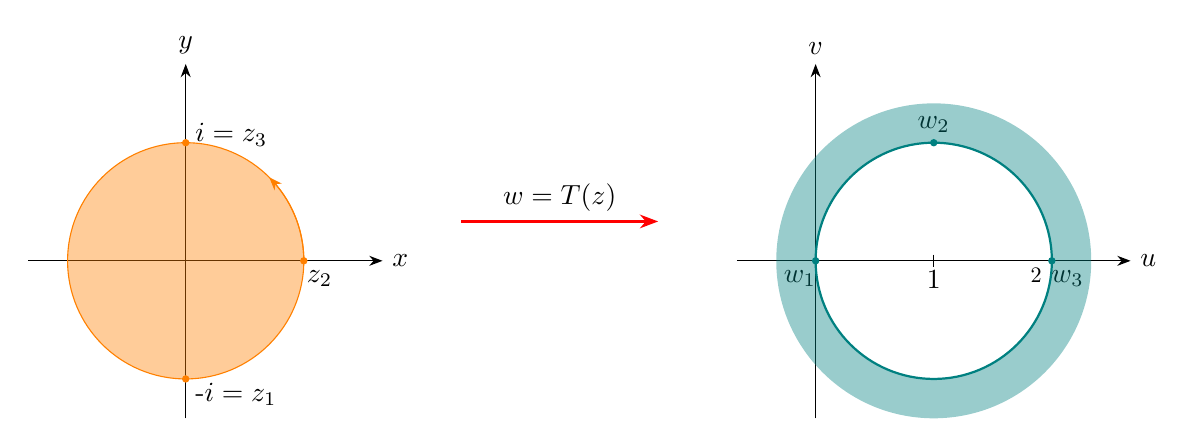
\begin{tikzpicture}[=>stealth]
\draw[-Stealth](-2,0)--(2.5,0)node[right]{$x$};
\draw[-Stealth](0,-2)--(0,2.5)node[above]{$y$};
\draw[orange,-Stealth](0,0)circle[radius=1.5cm];
\draw[orange,-Stealth](1.5,0)arc[start angle=0,end angle=45,radius=1.5cm];
\draw(0,-1.5)node[shape=circle,fill=orange,scale=0.01cm]{}
(0,1.5)node[shape=circle,fill=orange,scale=0.01cm]{}
(1.5,0)node[shape=circle,fill=orange,scale=0.01cm]{}
(0,1.6)node[right]{$i=z_3$}
(1.7,0)node[below]{$z_2$}
(0,-1.7)node[right]{-$i=z_1$}
(4.75,0.5)node[above]{$w=T(z)$};
\path[fill=orange,opacity=0.4](0,0)circle[radius=1.5cm];
\draw[thick,red,-Stealth](3.5,0.5)--(6,0.5);
\draw[-Stealth](7,0)--(12,0)node[right]{$u$};
\draw[-Stealth](8,-2)--(8,2.5)node[above]{$v$};
\draw[teal,thick](9.5,0)circle[radius=1.5cm];
\draw(9.5,0)node[below]{1}
(9.5,0.08)--(9.5,-0.08)
(8,0)node[shape=circle,fill=teal,scale=0.01cm]{}
(11,0)node[shape=circle,fill=teal,scale=0.01cm]{}
(9.5,1.5)node[shape=circle,fill=teal,scale=0.01cm]{}
(7.8,0)node[below]{$w_1$}
(11.2,0)node[below]{$w_3$}
(10.8,0)node[below,scale=0.8]{2}
(9.5,1.5)node[above]{$w_2$};
\path[fill=teal,opacity=0.4](11,0)arc[start angle = 0,end angle = 180,radius=1.5cm]--(8,0)--(7.5,0)arc[start angle = 180,end angle=0,radius = 2cm]--(11.5,0)--cycle
(7.5,0)arc[start angle =180,end angle = 360,radius=2cm]--(11.5,0)--(11,0)arc[start angle = 0,end angle = -180,radius=1.5cm]--(8,0)--(7.5,0)--cycle;
\end{tikzpicture}
\end{figure}















The interior of the circle $\hspace{0.2cm}\left|z\right| = 1\hspace{0.2cm}$ is mapped onto the exterior of the circle $\hspace{0.2cm}\left|w - 1\right|=1\hspace{0.2cm}$ in the $w-$plane.\\
This is because the LFT is conformal and so maintains the orientation.\\\\\\








\textbf{\textcolor{red}{Example}}\\
Show that the line $\hspace{0.2cm} 3y = x\hspace{0.2cm}$ is mapped onto the circle under the LFT $\hspace{0.2cm} w = \dfrac{iz + 2}{4z + i}.$ Find the centre and radius of the circle.\\
$\big[$Hint: Write $x$ and $y$ in terms of $u, v$ and use $\hspace{0.2cm} 3y  = x \big]$\\\\







\textbf{\textcolor{red}{Example}}\\
Find the LFT which maps 
\begin{enumerate}
\item[(a).] $\hspace{0.2cm} - 1, \hspace{0.2cm} 0, \hspace{0.2cm} 1\hspace{0.2cm}$ onto $\hspace{0.2cm} 0, \hspace{0.2cm} i, \hspace{0.2cm} 3i$

\item[(b).] $\hspace{0.2cm} i, \hspace{0.2cm} 1, \hspace{0.2cm} -1\hspace{0.2cm}$ onto $\hspace{0.2cm} 1, \hspace{0.2cm} 0, \hspace{0.2cm} \infty$
\end{enumerate}
respectively.\\\\





\textcolor{red}{Solution}
$$\dfrac{\big(w - w_1\big)\big(w_2 - w_3\big)}{\big(w - w_3\big)\big(w_2 - w_1\big)} = \dfrac{\big(z - z_1\big)\big(z_2 - z_3\big)}{\big(z - z_3\big)\big(z_2 - z_1\big)}$$

\begin{enumerate}
\item[(a).] So, we have that $\hspace{0.2cm} z_1 = 1,\hspace{0.2cm} z_2 = 0, \hspace{0.2cm} z_3 = 1\hspace{0.2cm}$ and $\hspace{0.2cm} w_1 = 0, \hspace{0.2cm} w_2 = i\hspace{0.2cm} w_3 = 3i$.

$$\implies\hspace{0.2cm} \dfrac{\big(z - z_1\big)\big(z_2 - z_3\big)}{\big(z - z_3\big)\big(z_2 - z_1\big)} = \dfrac{(z + 1) (-1)}{(z - 1) (+ 1)} = \dfrac{-(z + 1)}{(z - 1)} $$

and
$$\dfrac{\big(w - w_1\big)\big(w_2 - w_3\big)}{\big(w - w_3\big)\big(w_2 - w_1\big)} = \dfrac{(w - 0)(-2i)}{(w - 3i)(3i)} = \dfrac{(-2i)w}{3i(w - 3i)}$$
\begin{align*}
\implies \hspace{0.4cm} \dfrac{z + 1}{z - 1} & = \dfrac{2w}{3 (w - 3i)}\\\\
\implies \hspace{0.4cm} 3wz - 9zi + 3w - 9i & = 2wz - 2w\\
\implies\hspace{0.4cm} w & = \dfrac{9i ( z + 1)}{(z + 5)}
\end{align*}
Therefore, $\hspace{0.2cm} w = \dfrac{9i( z+ 1)}{z + 5}$\\



\item[(b).] We have that $\hspace{0.2cm} z_1 = i, \hspace{0.2cm} z_2 = 1, \hspace{0.2cm} z_3 = 0\hspace{0.2cm}$ and $\hspace{0.2cm} w_1 = 1, \hspace{0.2cm} w_2 = 0, \hspace{0.2cm} w_3 = \infty$
$$\implies \lim\limits_{w_3\rightarrow \infty}\hspace{0.3cm}\dfrac{\big(w - w_1\big)\big(w_2 - w_3\big)}{\big(w - w_3\big)\big(w_2 - w_1\big)} = \dfrac{w - w_1}{w_2 - w_1}$$


$$\implies \hspace{0.3cm} \dfrac{w - w_1}{w_2 - w_1} = \dfrac{w - 1}{-1} = -(w- 1)$$


$$\implies \hspace{0.3cm}\dfrac{\big(z - z_1\big)\big(z_2 - z_3\big)}{\big(z - z_3\big)\big(z_2 - z_1\big)} = \dfrac{(z - i)(1)}{(z)(1-i)} = \dfrac{(z - i)(1 + i)}{2z}$$\\


$\implies \hspace{0.3cm} -(w - 1)= \dfrac{(z - i)(1  + i)}{2z}$\\


$\implies \hspace{0.4cm} T(z) = w = 1 - \dfrac{(z - i)(1 + i)}{2z}$\\\\
\end{enumerate}













\textbf{\textcolor{red}{Example}}\\
Find a LFT that maps the crescent-shaped region that lies inside the circle $\hspace{0.2cm} \left|z - 2\right| < 2\hspace{0.2cm}$  and outside the circle $\hspace{0.2cm} \left|z - 1\right| > 1\hspace{0.2cm}$ onto a horizontal strip in the upper half plane.\\
$\big[$ Choose points $\hspace{0.2cm} z_1 = 4, \hspace{0.2cm} z_2 = 2 + 2i, \hspace{0.2cm}$ and $\hspace{0.2cm} z_3 = 0\hspace{0.2cm}$ on $\hspace{0.2cm}\left|z - 2\right| = 2\hspace{0.2cm}$ and $\hspace{0.2cm} w_1  = 0, \hspace{0.2cm} 1, \hspace{0.2cm}\\ w_3 = \infty\big]\hspace{0.2cm}$ Horizontal strip $\hspace{0.2cm} v = 1, \hspace{0.2cm} v = 0, \hspace{0.2cm} u>0$.
















\pagebreak
{\color[wave]{485}\section{Complex Integration}}


{\color[wave]{485}\subsection{Arc, Curve, Contour}}


\textbf{\textcolor{teal}{Definition}}\\
An arc in the complex plane $\mathbb{C}$ is defined to be an unbroken path of finite length.\\




\textbf{\textcolor{teal}{Definition}}\\
A path formed by joining together a number of arcs end$-$to$-$end in such way that the first path of the first arc coincides with the last point of arc is called a closed curve or contour.\\


We shall use simple curves (Jordan curve)

% DIAGRAM 1



\begin{table}[H]
\centering
\begin{tabular}{cccccccccccc}
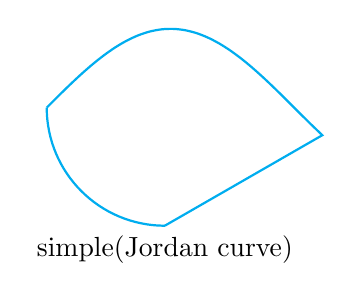
\begin{tikzpicture}
\draw[color=cyan,thick,domain=0:3.5,smooth,variable=\x]plot(\x,{sin(\x r)})--(1.5,-1.5);
\draw[color=cyan,thick](0,0)arc[start angle =180,end angle=270,radius=1.5cm];
\draw(1.5,-1.5)node[below]{simple(Jordan curve)};
\end{tikzpicture} &&&&&&&&&&&
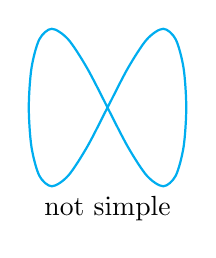
\begin{tikzpicture}
\draw[domain=-3.141:3.141,smooth,variable=\t,thick,cyan]plot({sin(\t r)},{sin(2*\t r)});
\draw(0,-1)node[below]{not simple};
\end{tikzpicture}\\
\end{tabular}
\end{table}

%\begin{figure}[H]
%\centering
%\begin{tikzpicture}
%\draw[color=cyan,thick,domain=0:3.5,smooth,variable=\x]plot(\x,{sin(\x r)})--(1.5,-1.5);
%\draw[color=cyan,thick](0,0)arc[start angle =180,end angle=270,radius=1.5cm];
%\draw(1.5,-1.5)node[below]{simple(Jordan curve)};
%\end{tikzpicture}
%\end{figure}


%\begin{figure}[H]
%\centering
%\begin{tikzpicture}
%\draw[domain=-3.141:3.141,smooth,variable=\t,thick,cyan]plot({sin(\t r)},{sin(2*\t r)});
%\draw(0,-1)node[below]{not simple};
%\end{tikzpicture}
%\end{figure}














\vspace{0.5cm}

\textbf{\textcolor{teal}{Parametric Representation}}\\
In the $z-$plane write $x$ and $y$ coordinates of the arc or curve in the parametric form $$x = x(s)\hspace{0.2cm}, \hspace{0.4cm} y = y(s)\hspace{0.7cm}\text{for}\hspace{0.3cm} \alpha \leq s\leq \beta\hspace{0.3cm}\cdots\cdots\cdots\hspace{0.3cm} (1)$$
where $x(s)$ and $y(s)$ are continuous for $C$ with parameter $s$.\\

Now, $z = x + iy$, by $(1)$ we have $z = z(s) = x(s) + iy(s)\hspace{0.3cm}\cdots\cdots\cdots\hspace{0.3cm} (2)\hspace{0.2cm}$ for $\alpha \leq s \leq \beta$.\\

Thus $ z(s_0) = x(s_0) + iy(s_0)$ is the point in the $z-$plane corresponding to $s = s_0$.\\

$z(\alpha)$ is the initial point and  $z(\beta)$ is the final point.


% DIAGRAM 2

\begin{figure}[H]
\centering
\begin{tikzpicture}[=>stealth]
%\draw[thick,cyan](0.5,1)..controls(2,1.8)and(3,1.3)..(4.5,1);
\draw[thick,cyan,out=-40](0.5,1)to(4.5,1);
\draw(0.5,1)node[shape=circle,fill=cyan,scale=0.01cm]{}
(4.5,1)node[shape=circle,fill=cyan,scale=0.01cm]{}
(0.5,-0.92)--(0.5,-1.08)
(4.5,-0.92)--(4.5,-1.08)
(0.5,-1.08)node[below]{$\alpha$}
(4.5,-1.08)node[below]{$\beta$};
\draw[-Stealth](-0.5,-1)--(5.5,-1);
\end{tikzpicture}
\end{figure}














\textbf{\textcolor{teal}{NOTE:}} The paramentarization creates a sense of direction on the curve.\\

If the curve contains no loops, then the simple curve is smooth when the derivatives $x'(s)$ and $y'(s)$ are continuous functions of $s$
$$z'(s) = x'(s) + iy'(s)\hspace{0.2cm}, \hspace{0.3cm} \alpha \leq s \leq \beta$$

The simple arc in $(1)$ is said to be piecewise smooth. When it is formed by a finite number of smooth segments joined at curves represented by the points $z(s_1), z(s_2), \cdots\cdots\cdots\cdots, z(s_n)$ with $\alpha \leq s_1< s_2< \cdots\cdots\cdots <s_n\leq \beta$.\\

We shall define the length of the simple arc $(1)$ by 
$$L = \int^{\beta}_{\alpha} \sqrt{x'(s)^2 + y'(s)^2}\hspace{0.1cm}ds$$\\






\textbf{\textcolor{red}{Example}}

%DIAGRAM 3


\begin{figure}[H]
\centering
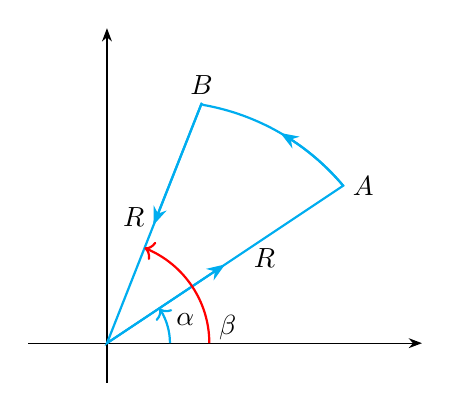
\begin{tikzpicture}[=>stealth]
\draw[-Stealth](-1,0)--(4,0);
\draw[-Stealth](0,-0.5)--(0,4);
\draw[thick,cyan](0,0)--(3,2)arc[start angle =40,end angle=80,radius=3cm]--(1.2,3.04)--cycle;
\draw[-Stealth,thick,cyan](0,0)--(1.5,1);
\draw[-Stealth,thick,cyan](3,2)arc[start angle=40,end angle = 60,radius=3cm];
\draw[-Stealth,thick,cyan](1.2,3.04)--(0.59,1.5);
\draw(3,2)node[right]{$A$}
(1.2,3.04)node[above]{$B$}
(2,1.33)node[below]{$R$}
(0.6,1.6)node[above,left]{$R$}
(1.3,0.2)node[right]{$\beta$};
\coordinate (a) at (1.5,1);
\coordinate (b) at (0,0);
\coordinate (c) at (0.59,1.5);
\coordinate (d) at (1.5,0);
\draw
pic[draw=cyan,thick,angle radius=0.8cm,->,angle eccentricity=1.3,"$\alpha$"]{angle=d--b--a};
\draw
pic[draw=red,thick,angle radius=1.3cm,->]{angle=d--b--c};
\end{tikzpicture}
\end{figure}


















Simple arc with initial point $A$ and final point $B$ can be parameterised as follows: $$x(\theta) = R\cos \theta;\hspace{0.5cm} y(\theta) = R\sin \theta;\hspace{0.5cm} \alpha \leq \theta \leq \beta$$
This arc is smooth because $x'(\theta)$ and $y'(\theta)$ are continuous functions of $\theta$. $$\left|z\right| = R\hspace{0.8cm} \text{on}\hspace{0.3cm}AB$$

The length of $AB$ is given by 
\begin{align*}
\int^{\beta}_{\alpha}\sqrt{\big(-R\sin \theta\big)^2 + \big(R\cos\theta\big)^2}\hspace{0.2cm}d\theta & = \int^{\beta}_{\alpha} R\sqrt{\sin^2\theta + \cos^2\theta}\hspace{0.2cm}d\theta\\
& =\int^{\beta}_{\alpha}R\hspace{0.1cm}d\theta\\\\
& = R\big(\beta - \alpha\big)\\\\
\end{align*}









{\color[wave]{485}\subsection{Contour Integration}}

% DIAGRAM 4

\begin{figure}[H]
\centering
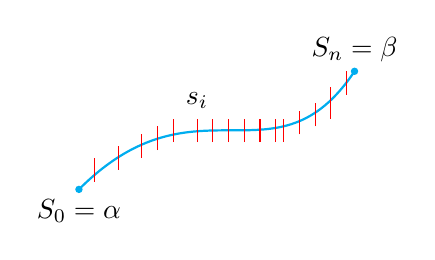
\begin{tikzpicture}[=>stealth]
\draw[thick,cyan](0.5,1)..controls(2,2.5)and(3,1)..(4,2.5);
\draw(4,2.5)node[shape=circle,scale=0.01cm,fill=cyan]{}
(0.5,1)node[shape=circle,scale=0.01cm,fill=cyan]{}
(4,2.5)node[above]{$S_n=\beta$}
(0.5,1)node[below]{$S_0=\alpha$};
\draw[red](0.7,1.1)--(0.7,1.4)
(1,1.25)--(1,1.55)
(1.3,1.4)--(1.3,1.7)
(1.5,1.5)--(1.5,1.8)
(1.7,1.6)--(1.7,1.9)
(2,1.6)--(2,1.9)node[above,black]{$s_i$}
(2.2,1.6)--(2.2,1.9)
(2.4,1.6)--(2.4,1.9)
(2.6,1.6)--(2.6,1.9)
(2.8,1.6)--(2.8,1.9)
(3,1.6)--(3,1.9)
(3.1,1.6)--(3.1,1.9)
(3.3,1.7)--(3.3,2)
(3.5,1.8)--(3.5,2.1)
(3.7,1.9)--(3.7,2.3)
(3.9,2.2)--(3.9,2.5);
\end{tikzpicture}
\end{figure}











Let $\hspace{0.2cm} z_{i-1} = z(s_{i-1})\hspace{0.1cm}$, writing $\Delta z_i = z_i - z_{i-1}$ and taking $z_i^*$ to be any point on the arc $C_i$, we form a sum $$S_n = \sum^n_{i=1} f\big(z^*_i\big)\Delta z_i$$
Let $f(z)$ be such that when $n\longrightarrow \infty\hspace{0.3cm}\max\left|\Delta z_i\right| \longrightarrow 0$, the complex number $S_n$ approaches a limit $S$ which is independent of the way the curve is partitioned.\\

We define $S$ as the integral of $f(z)$ with respect to $z$ taken as the  contour $C$ denoted by
$$S  = \int_r f(z)dz = \lim\limits_{n \rightarrow \infty} \Bigg[\sum^n_{i = 1} f\big(z^*_i\big)\Delta z_i \Bigg]$$


On the contour $C$, we write $\hspace{0.3cm}z(t) = x(t) + iy(t),\hspace{0.3cm} \alpha \leq t\leq \beta\hspace{0.2cm}\cdots\cdots\cdots\hspace{0.2cm}(1)$\\
Let $\hspace{0.2cm}f(t) = u(x,y) + iv(x,y)\hspace{0.2cm}$ where $u(x,y) = u\big(x(t), y(t)\big),\hspace{0.2cm} v(x,y) = v\big(x(t), y(t)\big)$ are piecewise continuous functions of $t$. Then 
$$\boxed{\int_Cf(z) dz = \int^{\beta}_{\alpha} f(z(t))\hspace{0.1cm}z'(t)dt\hspace{0.2cm}\cdots\cdots\cdots\hspace{0.3cm}(2)\\}$$

Since $f(z(t))z'(t) = \big[u(x(t),y(t)) + iy(x(t),y(t))\big]\big(x'(t) + iy'(t)\big)$ substitute this in $(2)$ then
$$\int_Cf(z)dz = \int^{\beta}_{\alpha} \big(ux' - vy'\big)dt + i\int^{\beta}_{\alpha}\big(vx' - uy'\big)dt\hspace{0.2cm}\cdots\cdots\cdots\hspace{0.2cm} (3)$$

In terms of the $x$ and $y$ as variables we have
$$\int_C f(z)dz = \int_C udx - vdy + i \int_Cvdx  + udy$$\\



\textbf{\textcolor{teal}{Proposition}}\\
Let $C$ be a piecewise smooth curve, and suppose that $f$ is continuous on $C$, then 
\begin{enumerate}
\item $\displaystyle{\int_Cf(z)dz = - \int_{C^-}f(z)dz}$

\item If $\gamma \in \mathbb{C}$, then $\displaystyle{\int_Cf(z)dz = \int\limits_{C + \gamma} f(z - \gamma)dz}$

\item $\displaystyle{\int_C Kf(z)dz = K\int_Cf(z)dz}, \hspace{0.2cm}K$ is constant.

\item $\displaystyle{\int_C\big[\alpha f(z)dz + \beta g(z)\big]dz = \alpha\int_Cf(z)dz + \beta \int_Cg(z)dz}$\\

If $C$ comprises of $n$ smooth arcs $C_1,C_2, \cdots\cdots\cdots, C_n$ joined end to end, then 
$$\int_Cf(z)dz = \int\limits_{C_1} f(z)dz + \cdots\cdots\cdots + \int\limits_{C_n} f(z)dz = \sum^n_{i = 1} \Bigg[\int\limits_{C_i} f(z)dz\Bigg]$$

\item If on a contour $C$ of length $L, \hspace{0.2cm}\left|f(z)\right|\leq \mu$, then 
\begin{align*}
\left|\int_Cf(z)dz\right| & \leq\int_C\left|f(z)\right|dz\\
& \leq \mu \int_Cdz\\
& = \mu L\\\\
\end{align*}
\end{enumerate}




\textbf{\textcolor{red}{Example}}\\
Consider the following diagram

% DIAGRAM 5

\begin{figure}[H]
\centering
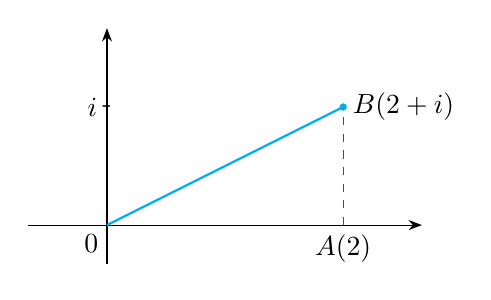
\begin{tikzpicture}[=>stealth]
\draw[-Stealth](-1,0)--(4,0);
\draw[-Stealth](0,-0.5)--(0,2.5);
\draw[thick,cyan](0,0)--(3,1.5);
\draw(-0.2,0)node[below]{0}
(3,0)node[below]{$A(2)$}
(3,1.5)node[right]{$B(2+i)$}
(0,1.5)node[]{-}
(0,1.5)node[left]{$i$}
(3,1.5)node[shape=circle,fill=cyan,scale=0.01cm]{};
\draw[dashed,red](3,0)--(3,1.49);
\end{tikzpicture}
\end{figure}
















Evaluate $\displaystyle{I = \int z^2 dz}$ on a smooth curve from point $O$ to point $B$.\\\\





\textcolor{red}{Solution}\\
If we evaluate $I$ along the straight line $OB$ with equation. We call this $\displaystyle{I_1 = \int\limits_{OB}z^2dz}$ $z = x + iy$ in terms of $y$. 
\begin{align*}
 z^2 & = (x + iy )^2  = (x^2 - y^2) + i 2xy\hspace{0.3cm} 0\leq y\leq 1\\
 & = (4y^2 - y^2) + i (2(2y)y)\\
 & = 3y^2 + i4y^2
\end{align*}



\begin{align*}
I_1 & = \int^1_0(3y^2 + 4y^2)(2+ i)dy\\
& = (3 + 4i)(2 + i) \int^1_0 y^2 dy\\
& = \dfrac{2}{3} + \dfrac{11}{3}i\\\\
\end{align*}







OR, we may evaluate $I$ via the path $OAB$, call it $I_2$
$$I_2 = \int\limits_{OA}z^2dz + \int\limits_{AB}z^2dz$$

Now, on $OA,\hspace{0.2cm} z(x) = x + 0i = x,\hspace{0.3cm} 0 \leq x \leq 2$\\

On $AB,\hspace{0.2cm} z(y) = 2 + yi,\hspace{0.3cm} 0\leq y \leq 1$
\begin{align*}
I_2 & = \int^2_0x^2dx + \int^1_0(2 + iy)^2dy\\
& = \dfrac{8}{3} + i\Bigg[\int^1_0(4 - y^2)dy + 4i\int^1_0ydy\Bigg]\\
& = \dfrac{8}{3} + i \Big(4 - \dfrac{1}{3}\Big) - 2\\
& = \dfrac{2}{3} + \dfrac{11}{3}i\\
\end{align*}



% DIAGRAM 6

\begin{figure}[H]
\centering
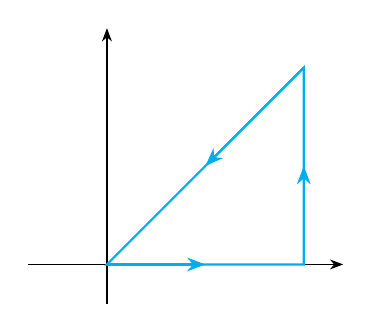
\begin{tikzpicture}[=>stealth]
\draw[-Stealth](-1,0)--(3,0);
\draw[-Stealth](0,-0.5)--(0,3);
\draw[-Stealth,thick,cyan](0,0)--(1.25,0);
\draw[-Stealth,thick,cyan](2.5,0)--(2.5,1.25);
\draw[-Stealth,thick,cyan](2.5,2.5)--(1.25,1.25);
\draw[thick,cyan](0,0)--(2.5,0)--(2.5,2.5)--cycle;
\end{tikzpicture}
\end{figure}












Note that $I_1 = I_2$, thus the value of $I$ is independent of path.\\

So if the question was to evaluate $\displaystyle{\int z^2 dz}$ around the closed path


% DIAGRAM 7

\begin{figure}[H]
\centering
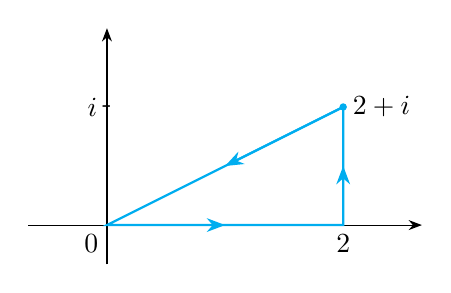
\begin{tikzpicture}[=>stealth]
\draw[-Stealth](-1,0)--(4,0);
\draw[-Stealth](0,-0.5)--(0,2.5);
\draw[-Stealth,thick,cyan](0,0)--(1.5,0);
\draw[-Stealth,thick,cyan](3,0)--(3,0.75);
\draw[-Stealth,thick,cyan](3,1.5)--(1.5,0.75);
\draw[thick,cyan](0,0)--(3,0)--(3,1.5)--cycle;
\draw(-0.2,0)node[below]{0}
(3,0)node[below]{$2$}
(3,1.5)node[right]{$2+i$}
(0,1.5)node[]{-}
(0,1.5)node[left]{$i$}
(3,1.5)node[shape=circle,fill=cyan,scale=0.01cm]{};
\end{tikzpicture}
\end{figure}











We have $I_1 - I_2 = 0$\\\\



\textbf{\textcolor{red}{Example}}\\
Evaluate $\displaystyle{\int_C \dfrac{dz}{z - z_0}}$ where $C$ is the contour around the region $\hspace{0.1cm}R_1 < \left|z - z_0\right| < R_2$.\\\\




\text{\textcolor{red}{Solution}}

% DIAGRAM 8


\begin{figure}[H]
\centering
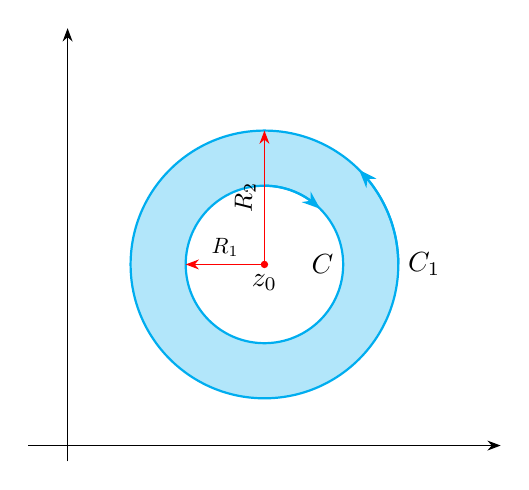
\begin{tikzpicture}[=>stealth]
\draw[-Stealth](-3,-2.3)--(3,-2.3);
\draw[-Stealth](-2.5,-2.5)--(-2.5,3);
\draw(0,0)node[shape=circle,scale=0.01cm,fill=red]{}
(0,0)node[below]{$z_0$}
(1,0)node[left]{$C$}
(1.7,0)node[right]{$C_1$};
\draw[thick,cyan](0,0)circle[radius=1cm];
\draw[thick,cyan](0,0)circle[radius=1.7cm];
\draw[-Stealth,thick,cyan](1.7,0)arc[start angle=0,end angle=45,radius=1.7cm];
\draw[-Stealth,thick,cyan](0,1)arc[start angle=90,end angle=45,radius=1cm];
\path[fill=cyan,opacity=0.3](1,0)arc[start angle=0,end angle=180,radius=1cm]--(-1,0)--(-1.7,0)--(-1.7,0)arc[start angle=180,end angle=0,radius=1.7cm]--(1.7,0)--cycle
(-1,0)arc[start angle=180,end angle=360,radius=1cm]--(1,0)--(1.7,0)--(1.7,0)arc[start angle=0,end angle=-180,radius=1.7cm]--(-1.7,0)--cycle;
\draw[-Stealth,red](0,0)--node[above,sloped,black,scale=0.8]{$R_1$}(-1,0);
\draw[-Stealth,red](0,0)--node[above,sloped,black,scale=0.9]{$R_2$}(0,1.7);
\end{tikzpicture}
\end{figure}












Clearly, $C$ denotes the inner and outer boundaries of the region
\begin{align*}
\int_C \dfrac{dz}{z - z_0} & = \int_{C_1} \dfrac{dz}{z - z_0} + \int_{C_2} \dfrac{dz}{z - z_0}\\\\
& = \int^{2\pi}_0\dfrac{iR_1e^{i\theta}d\theta}{R_1e^{i\theta}} + \int^{2\pi}_0 \dfrac{iR_2e^{i\theta}d\theta}{R_2e^{i\theta}}\\\\
& = i\int^{2\pi}_0d\theta + i \int^{2\pi}_0 d\theta\\\\
& = 2\pi i - 2\pi i \\
& = 0\\\\
\end{align*}








\textbf{\textcolor{red}{Example}}\\
Evaluate $\displaystyle{\int\big( z + 2\overline{z}\big)dz}$ where $C$ is the contour given by 

% DIAGRAM 9

\begin{figure}[H]
\centering
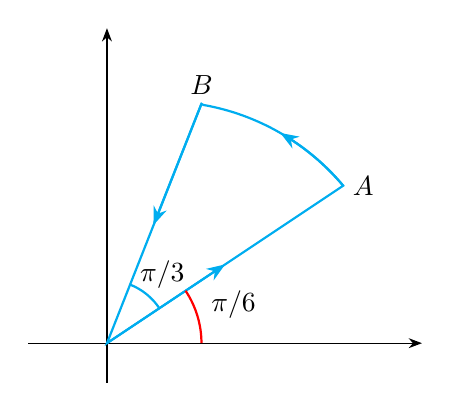
\begin{tikzpicture}[=>stealth]
\draw[-Stealth](-1,0)--(4,0);
\draw[-Stealth](0,-0.5)--(0,4);
\draw[thick,cyan](0,0)--(3,2)arc[start angle =40,end angle=80,radius=3cm]--(1.2,3.04)--cycle;
\draw[-Stealth,thick,cyan](0,0)--(1.5,1);
\draw[-Stealth,thick,cyan](3,2)arc[start angle=40,end angle = 60,radius=3cm];
\draw[-Stealth,thick,cyan](1.2,3.04)--(0.59,1.5);
\draw(3,2)node[right]{$A$}
(1.2,3.04)node[above]{$B$};
\coordinate (a) at (1.5,1);
\coordinate (b) at (0,0);
\coordinate (c) at (0.59,1.5);
\coordinate (d) at (1.5,0);
\draw
pic[draw=cyan,thick,angle radius=0.8cm,angle eccentricity=1.4,"$\pi/3$"]{angle=a--b--c};
\draw
pic[draw=red,thick,angle radius=1.2cm,angle eccentricity=1.4,"$\pi/6$"]{angle=d--b--a};
\end{tikzpicture}
\end{figure}













Here, contour $C$ is $OABC$.\\\\




\textbf{\textcolor{red}{Example}}\\
Evaluate $\displaystyle{\int \dfrac{dz}{z^{1/4}}}$ where $C$ is the circle $\left|z\right| = 1$
\begin{enumerate}
\item where the branch used is the axe $dz$. Where $1^{1/4} = -i$,
\item and the integration is to start from $z = i$.\\
\end{enumerate}




\text{\textcolor{red}{Working}}\\
We make $z^{1/4}$ single valued if $z = re^{i\theta}$, we see that for branches of $z^{1/4} = w$ are $$ w_k = r^{1/4}\exp \Bigg[i\dfrac{\theta_0 + 2k\pi)}{4} \Bigg],\hspace{0.3cm} k = 0, 1, 2, 3$$
Setting $z= 1$, so that $\left|z\right| = 1,\hspace{0.3cm} Arg(z) = 0$

\begin{align*}
\text{We get}\hspace{0.5cm} w_k(1) & = (1)^{1/4}\exp \Bigg(\dfrac{k\pi i}{2}\Bigg)\hspace{0.2cm} , \hspace{0.3cm} k = 0, 1, 2, 3\\\\
w_0(1) & = 1\\
w_1(1) & = i\\
w_2(1) & = -1\\
w_3(1) & = -i
\end{align*}

Now, since the center involves $\left|z\right|  = 1$, or $C$, we have $z = e^{i\theta}$ and $dz = ie^{i\theta}d\theta$
\begin{enumerate}
\item The branch to be selected is 
\begin{align*}
z^{1/4}  & = w_3(1) = r^{1/4} \exp \Bigg(i\Bigg(\dfrac{\theta + 2(3)\pi}{4}\Bigg)\Bigg)\\
& = r^{1/4} \exp\Big(\dfrac{i\theta_0}{4}\Big) \exp\Big(\dfrac{i6\pi}{4}\Big)\\
& = \exp \Big(\dfrac{i\theta_0}{4}\Big)(-i)\\
& = (-i)\exp \Big(\dfrac{i\theta_0}{4}\Big)\\
\end{align*}


\begin{align*}
\text{Thus}\hspace{0.3cm} \int_C \dfrac{1}{z^{1/4}}dz  & = \int_{\pi/2}^{5\pi/2}\dfrac{i e^{i\theta}}{-ie^{i\theta/4}}d\theta\\\\
& = - \int_{\pi/2}^{5\pi/2} e^{i3\theta/4}d\theta\\
\end{align*}




\item Start the integration from $z = 1$
\begin{align*}
\int_C \dfrac{1}{z^{1/4}}dz = \int^{2\pi}_0 \dfrac{i e^{i\theta}}{-ie^{i\theta/4}}d\theta\\
\end{align*}
\end{enumerate}






\textbf{\textcolor{red}{Examples}}
\begin{enumerate}
\item Evaluate $\displaystyle{\int_C \ln \overline{z}\hspace{0.1cm}dz}$ where $C$ is the unit circle $\left|z\right| = 1$. Use the branch $\ln 1 = 4\pi i$ and integration starts from $ z = 1$.

\item Show that $\displaystyle{\left|\displaystyle{\int_C \dfrac{e^{iz}}{z}}\right|\leq 2\pi e^R}$ where $C$ is $\left|z\right|  = R$\\\\
\end{enumerate}











{\color[wave]{485}\subsection{The Cauchy - Goursat Theorem}}

\textbf{\textcolor{teal}{Definition}}\\
We say that $z_0$ is a singular point of $f(z)$ if $f(z)$ is not analytic at $z_0$ but is differentiable in the neighbourhood of $z_0$.\\


\textbf{\textcolor{teal}{Definition}}\\
The point $z_0$ is a isolated singularity if $f(z)$ is analytic everywhere in the neighbourhood of $z_0$ except at $z_0$.\\\\





\textbf{\textcolor{red}{Examples}}
\begin{enumerate}
\item $f(z) = \dfrac{1}{z}\hspace{0.2cm},\hspace{0.1cm}$ singular point at $z = 0$, and is isolated.
\item $f(z) = \dfrac{z(3 + z)}{\big(z^2 + 4\big)\big(z^2 - 1\big)}\hspace{0.1cm},\hspace{0.1cm}$ singular points are $z = \pm 1,\hspace{0.2cm} \pm 2i$ and they are all isolated.
\item $f(z) = \dfrac{1}{\cos z}\hspace{0.2cm}$ singular points $z = \dfrac{n\pi}{2}, \hspace{0.3cm} n = \pm 1, \hspace{0.2cm} \pm 3, \hspace{0.2cm} 5,\hspace{0.2cm}\pm 7,\cdots\cdots\cdots\hspace{0.2cm}$ and they are all isolated.
\item $f(z) = \dfrac{1}{\sin \Big(\dfrac{1}{z}\Big)}\hspace{0.2cm}, \hspace{0.2cm}$ singular points $\dfrac{1}{z} = 0, \hspace{0.2cm} \pi, \hspace{0.2cm}, 2\pi, \hspace{0.2cm} 3\pi\hspace{0.2cm}\cdots\cdots$\\
$\implies \dfrac{1}{z} = n\pi, \hspace{0.2cm} n\in \mathbb{Z}$\\
$\implies z = \dfrac{1}{n\pi}\hspace{0.2cm},\hspace{0.2cm} n\in \mathbb{Z}$\\
and $z = 0$


% DIAGRAM 10


\begin{figure}[H]
\centering
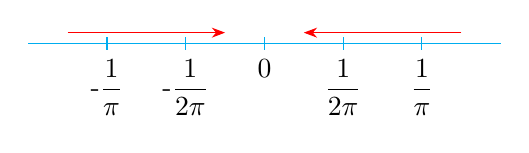
\begin{tikzpicture}[=>stealth]
\draw[cyan](-3,0)--(3,0)
(0,0.08)--(0,-0.08)node[below,black]{0}
(1,0.08)--(1,-0.08)node[below,black]{$\dfrac{1}{2\pi}$}
(2,0.08)--(2,-0.08)node[below,black]{$\dfrac{1}{\pi}$}
(-1,0.08)--(-1,-0.08)node[below,black]{-$\dfrac{1}{2\pi}$}
(-2,0.08)--(-2,-0.08)node[below,black]{-$\dfrac{1}{\pi}$};
\draw[-Stealth,red](-2.5,0.14)--(-0.5,0.14);
\draw[-Stealth,red](2.5,0.14)--(0.5,0.14);
\end{tikzpicture}
\end{figure}











Singularities of the form $z = \dfrac{1}{n\pi}$ are isolated but $z = 0$ is not.\\
\end{enumerate}




\textbf{\textcolor{teal}{Definition}}\\
A region $\Omega_x$ will be said to be $x-$simple if any line in $\Omega_x$ drawn parallel to $y-$axis crosses the boundary of $\Omega_x$ only twice.\\

Similarly, $\Omega_y$ is $y-$simple if a line drawn parallel to the $x-$axis only crosses the boundary twice.

% DIAGRAM 11

\begin{figure}[H]
\centering
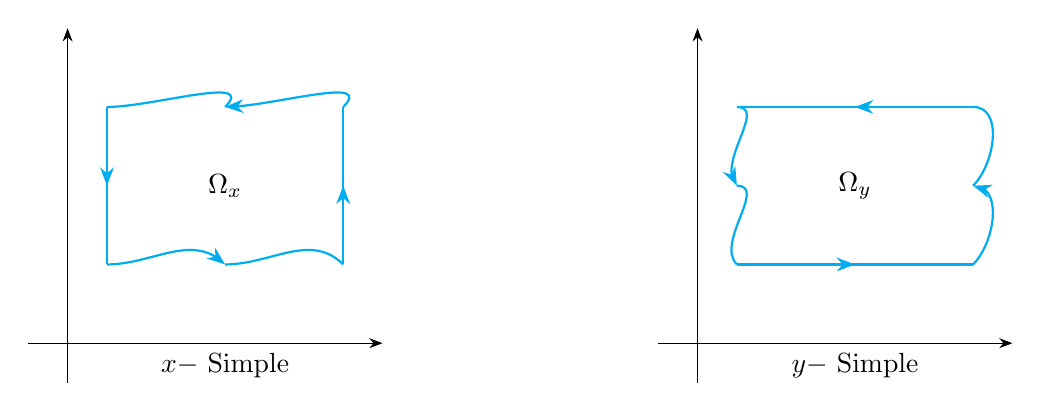
\begin{tikzpicture}[=>stealth]
\draw[-Stealth](-0.5,0)--(4,0);
\draw[-Stealth](0,-0.5)--(0,4);
\draw[thick,cyan](0.5,1)--(0.5,3)
(3.5,1)--(3.5,3);
\draw[-Stealth,thick,cyan,out=0](0.5,1)to(2,1);
\draw[thick,cyan,out=0](2,1)to(3.5,1);
\draw[-Stealth,thick,cyan](3.5,1)--(3.5,2);
\draw[-Stealth,thick,cyan](0.5,3)--(0.5,2);
\draw[-Stealth,thick,cyan,in=0](3.5,3)to(2,3);
\draw[thick,cyan,in=0](2,3)to(0.5,3);
\draw(2,2)node[]{$\Omega_x$}
(2,0)node[below]{$x-$ Simple};
%% y
\draw[-Stealth](7.5,0)--(12,0);
\draw[-Stealth](8,-0.5)--(8,4);
\draw[thick,cyan](8.5,1)--(11.5,1)
(8.5,3)--(11.5,3);
\draw[-Stealth,thick,cyan,out=0](8.5,3)to(8.5,2);
\draw[thick,cyan,out=0](8.5,2)to(8.5,1);
\draw[-Stealth,thick,cyan](8.5,1)--(10,1);
\draw[-Stealth,thick,cyan](11.5,3)--(10,3);
\draw[-Stealth,thick,cyan,in=0](11.5,1)to(11.5,2);
\draw[thick,cyan,in=0](11.5,2)to(11.5,3);
\draw(10,2)node[]{$\Omega_y$}
(10,0)node[below]{$y-$ Simple};
\end{tikzpicture}
\end{figure}











 If  a region is both $x-$simple and $y-$simple then it is said to be simple.\\\\
 
% DIAGRAM 12

\begin{figure}[H]
\centering
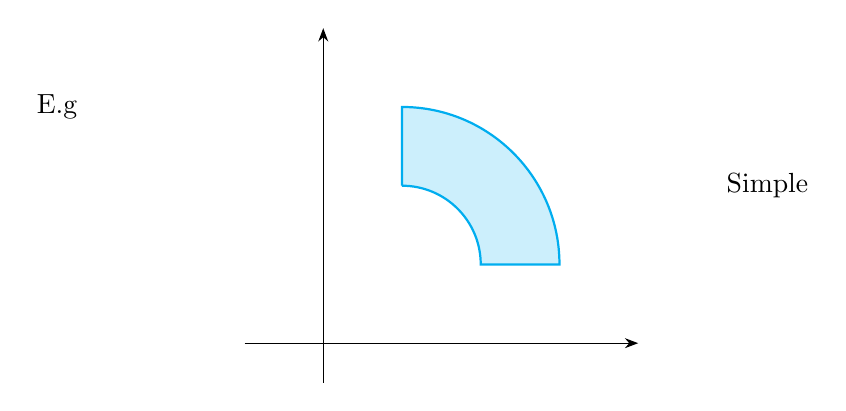
\begin{tikzpicture}[=>stealth]
\draw[-Stealth](-2,-1)--(3,-1);
\draw[-Stealth](-1,-1.5)--(-1,3);
\draw[thick,cyan](0,1)arc(90:0:1cm and 1cm)--(1,0)--(2,0)arc(0:90:2cm and 2cm)--(0,2)--(0,1);
\path[fill=cyan,opacity=0.2](0,1)arc(90:0:1cm and 1cm)--(1,0)--(2,0)arc(0:90:2cm and 2cm)--(0,2)--(0,1);
\draw(4,1)node[right]{Simple}
(-4,2)node[left]{E.g};
\end{tikzpicture}
\end{figure}












\vspace{1cm}
% DIAGRAM 13

\begin{figure}[H]
\centering

\begin{tikzpicture}[=>stealth]
\draw[thick,cyan](0,0)circle[radius=1cm];
\draw[thick,cyan](0,0)circle[radius=1.7cm];
\path[fill=cyan,opacity=0.3](1,0)arc[start angle=0,end angle=180,radius=1cm]--(-1,0)--(-1.7,0)--(-1.7,0)arc[start angle=180,end angle=0,radius=1.7cm]--(1.7,0)--cycle
(-1,0)arc[start angle=180,end angle=360,radius=1cm]--(1,0)--(1.7,0)--(1.7,0)arc[start angle=0,end angle=-180,radius=1.7cm]--(-1.7,0)--cycle;
\draw(4,0)node[right]{Not simple};
\end{tikzpicture}
\end{figure}














\textbf{\textcolor{teal}{Theorem: Green's Theorem for Simple Region}}\\
Let $\Omega$ be a simple region in the $xy-$plane with boundary $\Gamma$ oriented counter clockwise then if $P(x,y)$ and $Q(x,y)$ together with its partial derivatives are continuous in $\Omega$, then $$ \iint\limits_{\Omega} \Bigg(\dfrac{\partial Q}{\partial x} - \dfrac{\partial P}{\partial y}\Bigg)dxdy = \int\limits_{\Gamma} \Big[Pdx + Qdy\Big]$$\\

\textbf{\textcolor{teal}{Proof:}} Research\\\\




\textbf{\textcolor{teal}{Theorem: Cauchy - Goursat}}\\
If $f(z)$ is analytic in a simply connected region $D$ and also on its boundary $C$ which is a smooth closed curve, then $$\ointctrclockwise_C f(z) dz = 0$$



\textbf{\textcolor{teal}{Proof}}\\
If $f(z) = u + iv$, then $\displaystyle{\ointctrclockwise_C f(z) dz = \int_C \Big[ u dx - vdy\Big] + i \int_C \Big[udy + vdx\Big]}$\\
Assuming $f(z)$ and $f'(z)$ are continuous. Then we can apply Green's theorem
$$\implies\hspace{0.5cm} \int_Cf(z) dz = - \iint\limits_D \Bigg(\dfrac{\partial v}{\partial x} + \dfrac{\partial u}{\partial y}\Bigg) dxdy + i \iint\limits_D \Bigg(\dfrac{\partial u}{\partial x} - \dfrac{\partial v}{\partial y}\Bigg)dxdy$$
Since $f(z)$ is analytic in $D$, it satisfies the Cauchy - Riemann equations. Thus $$\int_C f(z) dz = 0$$.\\





\textbf{\textcolor{teal}{Theorem: ( Generalised Cauchy - Goursat)}}\\
Let the domain $D$ be bounded externally by a simple closed contour $C_0$ and internally by non intersecting closed contours $C_1, C_2, \cdots\cdots\cdots,  C_n$. Let both the external and internal contours be positively oriented. Then if $f(z)$ is analytic in $D$ then $$ \int_{C_0} f(z)dz = \sum^n_{r = 1} \int_{C_r}f(z)dz$$\\







\textbf{\textcolor{red}{Example}}\\
Evaluate $\displaystyle{\int_C \dfrac{\big(4 - 2i\big) z^2 + \big(2 - 5i\big) z + \big(3 - 2i\big)}{\big(z^2 + 1\big)\big(z + 2\big)}dz}$  where
\begin{enumerate}
\item $C$ is the square $C_1$ with corners $\dfrac{1}{2}+ \dfrac{1}{2}i\hspace{0.2cm}, \hspace{0.3cm} \dfrac{-1}{2}+ \dfrac{1}{2}i\hspace{0.2cm}, \hspace{0.3cm} \dfrac{-1}{2} - \dfrac{1}{2}i\hspace{0.2cm}, \hspace{0.3cm} \dfrac{1}{2}-\dfrac{1}{2}i$
\item $C$ is the unit circle $C_2$ centered on $z = i$.
\item $C$ is the unit circle $C_3$ centered at $z = -2$.\\\\
\end{enumerate}





\text{\textcolor{red}{Working}}
\begin{enumerate}
\item

% DIAGRAM 14

\begin{figure}[H]
\centering
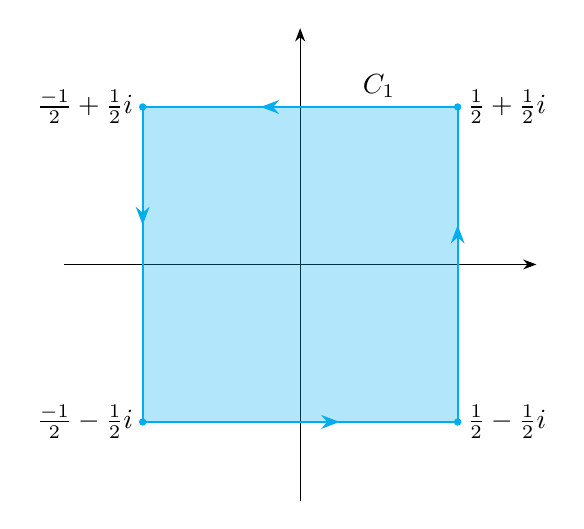
\begin{tikzpicture}[=>stealth]
\draw[-Stealth](-3,0)--(3,0);
\draw[-Stealth](0,-3)--(0,3);
\draw(-2,2)node[shape=circle,scale=0.01cm,fill=cyan]{}
(-2,-2)node[shape=circle,scale=0.01cm,fill=cyan]{}
(2,2)node[shape=circle,scale=0.01cm,fill=cyan]{}
(2,-2)node[shape=circle,scale=0.01cm,fill=cyan]{}
(2,-2)node[right]{$\frac{1}{2}-\frac{1}{2}i$}
(2,2)node[right]{$\frac{1}{2}+\frac{1}{2}i$}
(-2,2)node[left]{$\frac{-1}{2}+\frac{1}{2}i$}
(-2,-2)node[left]{$\frac{-1}{2}-\frac{1}{2}i$}
(1,2)node[above]{$C_1$};
\draw[-Stealth,thick,cyan](2,0)--(2,0.5);
\draw[-Stealth,thick,cyan](0,2)--(-0.5,2);
\draw[-Stealth,thick,cyan](-2,2)--(-2,0.5);
\draw[-Stealth,thick,cyan](0,-2)--(0.5,-2);
\draw[thick,cyan](2,2)--(-2,2)--(-2,-2)--(2,-2)--cycle;
\path[fill=cyan,opacity=0.3](2,2)--(-2,2)--(-2,-2)--(2,-2)--cycle;
\end{tikzpicture}
\end{figure}












We first check if $\displaystyle{ \dfrac{\big(4 - 2i\big) z^2 + \big(2 - 5i\big) z + \big(3 - 2i\big)}{\big(z^2 + 1\big)\big(z + 2\big)}}$ is analytic inside the region enclosed by $C_1$. $f(z)$ has singularities at $z = \pm i,\hspace{0.2cm} z = -2,\hspace{0.2cm}$, clearly are not in the enclosed  region. Thus $f(z)$ is analytic in the region. By Cauchy Goursat we have
$$\int_{C_1} f(z)dz = 0$$

\item

% DIAGRAM 15

\begin{figure}[H]
\centering
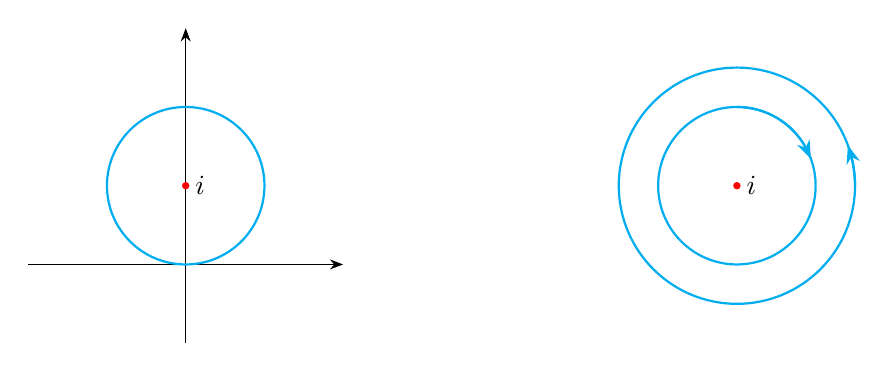
\begin{tikzpicture}[=>stealth]
\draw[-Stealth](-2,0)--(2,0);
\draw[-Stealth](0,-1)--(0,3);
\draw[thick,cyan](0,1)circle[radius=1cm];
\draw(0,1)node[shape=circle,fill=red,scale=0.01cm]{}
(0,1)node[right]{$i$}
(7,1)node[shape=circle,fill=red,scale=0.01cm]{}
(7,1)node[right]{$i$};
\draw[cyan,thick](7,1)circle[radius=1cm];
\draw[cyan,thick](7,1)circle[radius=1.5cm];
\draw[-Stealth,thick,cyan](7,2)arc[start angle=90,end angle=20,radius=1cm];
\draw[-Stealth,thick,cyan](8.5,1)arc[start angle = 0,end angle= 20,radius=1.5cm];
\end{tikzpicture}
\end{figure}





















Clearly $i$ is in the enclosed region. Thus by  Cauchy Goursat $\hspace{0.3cm} \displaystyle{\int_{C_2} f(z)dz = \sum^1_{r=1} \int f(z)dz}$
$$f(z) = \dfrac{-i}{z - i} + \dfrac{1 + i}{z + i} + \dfrac{3}{z + 2}$$

So that $\hspace{0.3cm} \displaystyle{\int_{C_2}f(z)dz = -i \int_{C_2} \dfrac{1}{z - i}dz + \big(1 + i\big)\underbrace{\int_{C_2} \dfrac{1}{z + i}dz}_0 + 3 \underbrace{\int_{C_2}\dfrac{1}{z + 2}dz}_0}$


\begin{align*}
\therefore\hspace{0.5cm} \int_Cf(z) dz  & = - i \int_{C_2} \dfrac{1}{z - i}dz\\
& = -i \int^{2\pi}_0\\
& = 2\pi\\
\end{align*}




\item When $C$ is the unit circle $C_3$ centered on $z = -2$

% DIAGRAM 16

\begin{figure}[H]
\centering
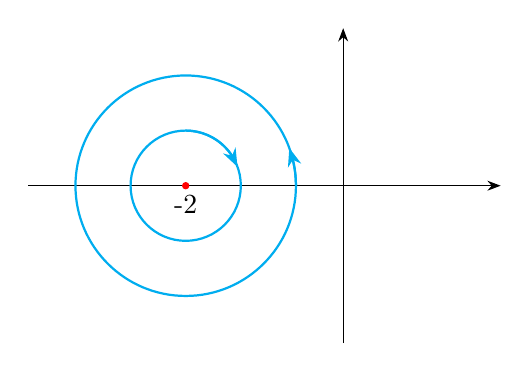
\begin{tikzpicture}[=>stealth]
\draw[-Stealth](-4,0)--(2,0);
\draw[-Stealth](0,-2)--(0,2);
\draw(-2,0)node[shape=circle,fill=red,scale=0.01cm]{}
(-2,0)node[below]{-2};
\draw[cyan,thick](-2,0)circle[radius=0.7cm];
\draw[cyan,thick](-2,0)circle[radius=1.4cm];
\draw[-Stealth,thick,cyan](-2,0.7)arc[start angle=90,end angle=20,radius=0.7cm];
\draw[-Stealth,thick,cyan](-0.6,0)arc[start angle = 0,end angle= 20,radius=1.4cm];
\end{tikzpicture}
\end{figure}











\begin{align*}
\text{Thus}\hspace{0.3cm} \int_{C_3}f(z)dz & = 0 + 0 + \int_{C_3} \dfrac{1}{z + 2}dz\\
& = 3(2\pi i)\\
& = 6\pi i\\\\
\end{align*}
\end{enumerate}








\textbf{\textcolor{red}{Example}}\\
Evaluate $\displaystyle{\int_C\dfrac{z^2 + \big(10- i\big)z - \big(4 + 2i\big)}{\big(z^2 + 1\big)\big(z + 2\big)}dz}$ where $C$ is the circle $\left|z\right|  = 3$.\\


Singular points are $\hspace{0.2cm} z = \pm i, \hspace{0.2cm} z = -2$

% DIAGRAM 17

\begin{figure}[H]
\centering
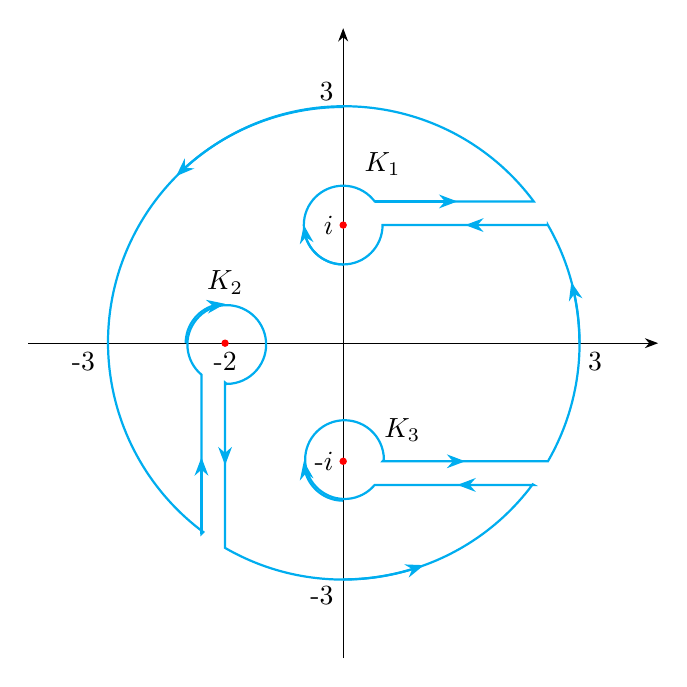
\begin{tikzpicture}[=>stealth]
\draw[-Stealth](-4,0)--(4,0);
\draw[-Stealth](0,-4)--(0,4);
\draw(0,1.5)node[shape=circle,scale=0.01cm,fill=red]{}
(0,-1.5)node[shape=circle,scale=0.01cm,fill=red]{}
(-1.5,0)node[shape=circle,scale=0.01cm,fill=red]{}
(0,1.5)node[left]{$i$}
(0,-1.5)node[left]{-$i$}
(-1.5,0)node[below]{-2}
(0.4,-1.1)node[right]{$K_3$}
(-1.5,0.5)node[above]{$K_2$}
(0.5,2)node[above]{$K_1$};
\draw[-Stealth,thick,cyan](3,0)arc[start angle=0,end angle=15,radius=3cm];
\draw[-Stealth,thick,cyan](0,3)arc[start angle=90,end angle=135, radius=3cm];
\draw[-Stealth,thick,cyan](0,-3)arc[start angle=270,end angle=290,radius=3cm];
%% K_1
\draw[-Stealth,thick,cyan](2.6,1.5)--(1.55,1.5);
\draw[-Stealth,thick,cyan](0.4,1.8)--(1.45,1.8);
\draw[-Stealth,thick,cyan](0,1)arc[start angle = -90,end angle=-180,radius=0.5cm];
%% K_3
\draw[-Stealth,thick,cyan](0.5,-1.5)--(1.55,-1.5);
\draw[-Stealth,thick,cyan](2.42,-1.8)--(1.45,-1.8);
\draw[-Stealth,thick,cyan](0,-2)arc[start angle=-90,end angle=-180,radius=0.5cm];
%% K_2
\draw[-Stealth,thick,cyan](-1.8,-2.42)--(-1.8,-1.45);
\draw[-Stealth,thick,cyan](-1.5,-0.5)--(-1.5,-1.55);
\draw[-Stealth,thick,cyan](-2,0)arc[start angle=180,end angle=90,radius=0.5cm];
\draw[thick,cyan](2.42,1.8)arc[start angle=36.65, end angle=233.35,radius=3cm]--(-1.8,-2.42)--(-1.8,-0.4)arc[start angle=230,end angle=-90,radius=0.5cm]--(-1.5,-0.5)--(-1.5,-2.6)arc[start angle = 240,end angle = 323.35,radius=3cm]--(2.42,-1.8)--(0.4,-1.8)arc[start angle=-40,end angle=-360,radius=0.5cm]--(0.5,-1.5)--(2.6,-1.5)--(2.6,-1.5)arc[start angle=330,end angle=390,radius=3cm]--(2.6,1.5)--(0.5,1.5)arc[start angle=360,end angle=40,radius=0.5cm]--(0.4,1.8)--(2.42,1.8)--(2.42,1.8)arc[start angle=36.65, end angle=180,radius=3cm];
%%
\draw(3.2,0)node[below]{3}
(-3.3,0)node[below]{-3}
(0,3.2)node[left]{3}
(0,-3.2)node[left]{-3};
\end{tikzpicture}
\end{figure}














Let $K_1, K_2, K_3$ be the closed contours as shown. Since $f(z)$ is analytic in $D$, thus by Cauchy - Goursat

$$\int_C f(z) dz = \int_{K_1}f(z)dz + \int_{K_2}f(z)dz + \int_{K_3}f(z)dz$$\\

$$f(z) = \dfrac{2}{z  - i} + \dfrac{3}{z + i} - \dfrac{4}{z + 2}$$


\begin{align*}
\therefore\hspace{0.3cm} \int_C f(z)dz & = 2 \int_{K_1} \dfrac{1}{z  - i}dz - \int_{K_2}\dfrac{1}{z + 2}dz + 3\int_{K_3}\dfrac{1}{z + i}dz\\\\
& = 2\big(2\pi i\big) - 4\big(2\pi i\big) + 3\big(2\pi i\big)\\\\
& = 2\pi i\\\\
\end{align*}








{\color[wave]{485}\subsection{Antiderivatives}}

\textbf{\textcolor{teal}{Theorem (Antiderivatives)}}\\
Let the complex function $f(z)$ be analytic in a simply connected region $D$. Then if $\gamma$ is any are lying entirely within $D$ with initial point $z_0$ and terminal point $z$, the antiderivative $$ F(z) = \int_{\gamma} f(\zeta)d\zeta = \int^{z}_{z_0} f(\zeta) d\zeta\hspace{0.3cm}\text{is a single valued function}$$


Clearly, this function is analytic in $D$ depending on $z$ but is independent of the arc $\gamma$. We have $F'(z) = f(z)$.\\


\textbf{\textcolor{teal}{Proof}}\\
Consider $\hspace{0.3cm} \displaystyle{\lim\limits_{h \rightarrow 0}\left|\dfrac{F(z + h) - F(z)}{h} - f(z)\right|}$\\\\ 
We want to show that the limit of the above expression is 0 for all $z \in D$.\\

We have that
\begin{align*}
\dfrac{F(z + h) - F(z)}{h} & = \dfrac{1}{h} \int^{z + h}_{z_0} f(\zeta) d\zeta - \dfrac{1}{h}\int^z_{z_0} f(\zeta)d\zeta\\\\
& = \dfrac{1}{h}\int^{z + h}_zf(\zeta) d\zeta \hspace{0.3cm} \cdots\cdots\cdots\hspace{0.5cm} (*)
\end{align*}
Choose the arc joining $z + 0\hspace{0.2cm} z + h$ to be straight line $\hspace{0.3cm} \displaystyle{\int^{z+h}_zd\zeta = h}$\\

\begin{align*}
\text{Now, write}\hspace{0.4cm} f(z) & = \dfrac{f(z)}{h}\cdot h = \dfrac{f(z)}{h}\int_z^{z + h} d\zeta\\\\
& = \dfrac{1}{h}\int^{z + h}_z f(z)d\zeta \hspace{0.5cm}\cdots\cdots\cdots\hspace{0.3cm}(**)
\end{align*}


Thus by $(*)$ and $(**)$ we have
\begin{align*}
\left|\dfrac{F(z + h) - F(z)}{h} - f(z)\right| & = \left|\dfrac{1}{h}\displaystyle{\int^{z +h}_z f(\zeta) d\zeta - \dfrac{1}{h}\int^{z + h}_z f(z)d\zeta}\right|\\\\
& = \dfrac{1}{\left|h\right|
}\left|\displaystyle{\int^{z + h}_z \big( f(\zeta) - f(z)\big) d\zeta}\right|\\\\
& \leq \dfrac{1}{\left|h\right|} \max\limits_{\zeta \in \gamma}\left|f(\zeta) - f(z)\right|\left|\displaystyle{\int^{z + h}_z d\zeta}\right|\\\\
& = \dfrac{1}{\left|h\right|}\hspace{0.1cm}\max\limits_{\zeta \in \gamma} \left|f(\zeta) - f(z)\right|\hspace{0.1cm}\left|h\right|\\\\
& = \max\limits_{\zeta\in \gamma}\left|f(\zeta) - f(z)\right|\\
\end{align*}

But $f(z)$ is continuous in $D$. So that $\hspace{0.2cm} \displaystyle{\lim\limits_{h\rightarrow 0} \hspace{0.1cm}\max\limits_{\zeta \in D} \left|f(\zeta) - f(z)\right| = 0}.\hspace{0.3cm}$\\ Hence $F'(z) = f(z)$\\\\\\









\pagebreak

{\color[wave]{485}\subsection{Definite Integral}}

\textbf{\textcolor{teal}{Theorem ( Definite Integral)}}\\
Let $f(z)$ be analytic in a simply connected domain $D$, let $F(z)$ be an antiderivative of $f(fz)$. Then for any two points $z_0, \hspace{0.2cm} z_1$; in $D$ $$\int_{z_0}^{z_1} f(z)dz = F(z_1) - F(z_0)$$\\





\textbf{\textcolor{red}{Example}}\\
Evaluate\\


\begin{enumerate}
\item $\displaystyle{\int_{1 + i}^{2 + i} e^{2z}dz}$\\

$f(z) = e^{2z}\hspace{0.3cm}, \hspace{0.3cm} F(z) = \dfrac{1}{2}e^{2z}$\\

$\displaystyle{\int_{1 + i}^{2 + i} e^{2z}dz  = \dfrac{1}{2}e^{2(2+i)} - \dfrac{1}{2}e^{2(1 + i)} = \dfrac{1}{2}e^{2i}\Big[ e^4 - e^2\Big]}$\\\\



\item $\displaystyle{\int_1^{2 + 3i} \sinh 3z dz}$\\

$f(z) = \sinh 3z\hspace{0.3cm}, \hspace{0.3cm} F(z) = \dfrac{1}{3}\cosh 3z$

\begin{align*}
\int_1^{2 + 3i} \sinh 3z dz & = \dfrac{1}{3}\cosh 3(2  + 3i) - \dfrac{1}{3}\cosh 3(i)\\\\
& = \dfrac{1}{3}\Bigg[\dfrac{e^{3(2 + 3i)} + e^{-3(2 + 3i)}}{2}  - \dfrac{e^3 + e^{-3}}{2}\Bigg]\\\\
\end{align*}
\end{enumerate}









{\color[wave]{485}\subsection{The Cauchy Integral Formula}}

\textbf{\textcolor{teal}{Theorem (Cauchy Integral Formula)}}\\
If $f(z)$ is analytic in a simply connected domain $D$ containing a simple closed contour $C$ and $z_0$ is any point in the interior of $C$, then $$ f(z_0) = \dfrac{1}{2\pi i} \int_C \dfrac{f(z)}{z - z_0}dz$$\\




\textbf{\textcolor{red}{Example}}\\
Evaluate $\displaystyle{\int_C \dfrac{ze^{-z}}{z - \dfrac{i \pi}{2}}dz},\hspace{0.2cm}$ where $C$ is the triangle with vertices $\hspace{0.2cm} -1-i, \hspace{0.2cm} 1 - i, \hspace{0.2cm} 2i$\\

\text{\textcolor{red}{Solution}}

% DIAGRAM 18

\begin{figure}[H]
\centering
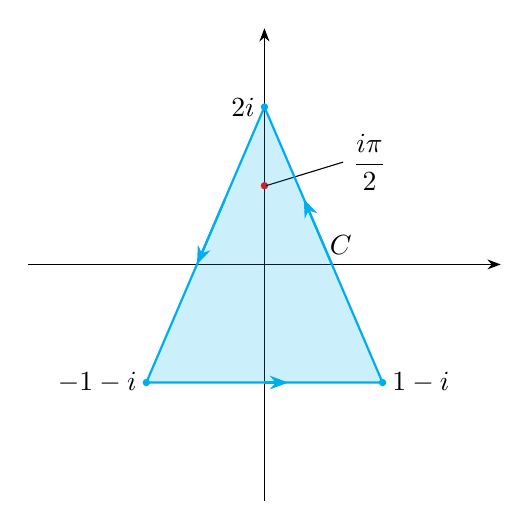
\begin{tikzpicture}[=>stealth]
\draw[-Stealth](-3,0)--(3,0);
\draw[-Stealth](0,-3)--(0,3);
\draw(0,2)node[shape=circle,fill=cyan,scale=0.01cm]{}
(-1.5,-1.5)node[shape=circle,fill=cyan,scale=0.01cm]{}
(1.5,-1.5)node[shape=circle,fill=cyan,scale=0.01cm]{}
(0,2)node[left]{$2i$}
(-1.5,-1.5)node[left]{$-1-i$}
(1.5,-1.5)node[right]{$1-i$}
(0,1)node[shape=circle,fill=red,scale=0.01cm]{}
(0.97,0)node[above]{$C$};
\draw(0.02,1)--(1,1.3)node[right]{$\dfrac{i\pi}{2}$};
\draw[-Stealth,thick,cyan](0.857,0)--(0.5,0.83);
\draw[-Stealth,thick,cyan](0,-1.5)--(0.3,-1.5);
\draw[-Stealth,thick,cyan](-0.5,0.83)--(-0.857,0);
\draw[thick,cyan](0,2)--(-1.5,-1.5)--(1.5,-1.5)--cycle;
\path[fill=cyan,opacity=0.2](0,2)--(-1.5,-1.5)--(1.5,-1.5)--cycle;
\end{tikzpicture}
\end{figure}













Take $f(z) = z e^{-z}, \hspace{0.3cm} z_0 = \dfrac{i\pi}{2}$
\begin{align*}
\int_C \dfrac{ze^{-z}}{z - \dfrac{i \pi}{2}}dz & = 2\pi i \cdot ze^{-z}\Big|_{z = i\dfrac{\pi}{2}}\\
& = 2\pi i \cdot \dfrac{i \pi}{2}e^{-i\pi/ 2}\\
& = -\pi^2\\\\
\end{align*}










\textbf{\textcolor{blue}{Exercise}}\\
Evaluate $\displaystyle{\int_C \dfrac{e^{-z}}{z^3 + 2z^2 - 3z - 10}}dz\hspace{0.1cm}$, where $C$ is the triangle with vertices $\hspace{0.2cm} i, \hspace{0.2cm} -i, $ and $3$.\\\\\\







\textbf{\textcolor{red}{Example}}\\
Evaluate $\displaystyle{\int_C \dfrac{e^{iz}}{z^2 + a^2}dz\hspace{0.2cm}, \hspace{0.2cm}}$ where $C$ is the circle $\left|z - ia\right| = a, \hspace{0.3cm} a\in \mathbb{R}$.\\


\text{\textcolor{red}{Solution}}\\
$z^2 + a^2 = (z - ia) (z + ia)$, hence singular points at $z = ia$ and $z = -ia$

% DIAGRAM 20

\begin{figure}[H]
\centering
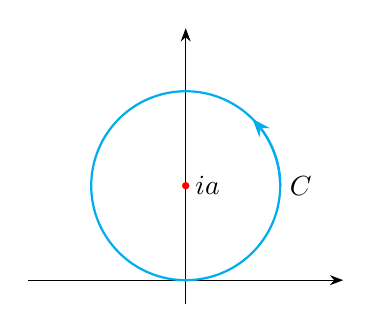
\begin{tikzpicture}[=>stealth]
\draw[-Stealth](-2,-1.2)--(2,-1.2);
\draw[-Stealth](0,-1.5)--(0,2);
\draw[thick,cyan](0,0)circle[radius=1.2cm];
\draw[thick,cyan,-Stealth](1.2,0)arc[start angle=0,end angle=45,radius=1.2cm];
\draw(0,0)node[shape=circle,fill=red,scale=0.01cm]{}
(0,0)node[right]{$ia$}
(1.2,0)node[right]{$C$};
\end{tikzpicture}
\end{figure}















$ia$ lies in the interior of $C$,
\begin{align*}
\int_C \dfrac{e^{iz}}{z^2 + a^2}dz & = \int_C \dfrac{e^{iz}}{(z - ia)(z + ia)}dz\\\\
& = \int_C \dfrac{e^{iz}/z + ia}{z - ia} dz\\\\
& = 2\pi i \cdot \dfrac{e^{iz}}{z + ia}\Bigg|_{z = ia}\\\\
& = \dfrac{2\pi i \cdot e^{-a}}{2ia}\\\\
& = \dfrac{\pi}{ae^a}\\\\
\end{align*} 


Suppose we used the Cauchy Goursat 
\begin{align*}
\int_C \dfrac{e^{iz}}{z^2 + a^2}dz & = \int_c \dfrac{e^{iz}}{(z - ia) (z + ia)}dz\\\\
& = \int_C \dfrac{A}{z - ia}dz + \int_C \dfrac{B}{z + ia}dz\\ 
\end{align*}


$$e^{iz} = A(z + ia) + B(z - ia)$$

Let $z = ia, \hspace{0.3cm} e^{-a} = 2aiA \implies A= \dfrac{1}{2iae^a}$\\

Let $z = - ia, \hspace{0.3cm} e^a = -2iaB \implies B = \dfrac{-e^a}{2ia}$




\begin{align*}
\int_C \dfrac{e^{iz}}{z^2 + a^2}dz  & = \int_C \dfrac{e^{iz}/2iae^a}{z - ia}dz + \underbrace{\int_C \dfrac{-e^{a}/2ia}{z + ia}dz}_0\hspace{0.3cm}\text{since}\hspace{0.2cm}\dfrac{e^{-a}/2ia}{z + ia}\hspace{0.3cm} \text{is analytic inside}\hspace{0.2cm}C\\\\
& = \dfrac{1}{2iae^a}\int_C \dfrac{1}{z - ia}dz\\\\
& = \dfrac{1}{2iae^a}\cdot 2\pi i\\\\
& = \dfrac{\pi}{ae^a}\\\\
\end{align*}




\textbf{\textcolor{blue}{Exercise}}
\begin{enumerate}
\item Locate the singular points and state their nature
\begin{enumerate}
      \item $\displaystyle{f(z) = \dfrac{1}{\sinh\Big(\dfrac{1}{z}\Big)}}$\\
      
      \item $\displaystyle{f(z) = \dfrac{1 + z}{\big(z^2 + 4\big)\sin z}}$\\
\end{enumerate}


\item Evaluate $\displaystyle{\int_C \dfrac{4z^2 + 9iz + 27}{z \big( z^2 + 9\big)}dz\hspace{0.2cm}}$ where $C$ is the common perimeter of the circles\\ $\left|z - 3\right| = 4, \hspace{0.2cm} \left|z + 2\right|  = 3$\\\\
\end{enumerate}





\textbf{\textcolor{teal}{The Cauchy Integral Formula Applied to Integrals of Trigonometric Functions}}\\
One of the applications of the Cauchy integral formula is the evaluation of real integrals of the form $$I = \int^{2\pi}_0 F\big(\sin x, \cos x\big) dx$$
In which the integrad is the quotient of two polynomials in $\sin x$ and $\cos x$, i.e
$$\int \dfrac{1}{2 + \cos x}\hspace{0.1cm}dx \hspace{0.5cm}, \hspace{0.5cm} \int \dfrac{1}{a^2 + \sin^2 x}\hspace{0.1cm}dx$$

The approach is as follows:
\begin{enumerate}
\item Set 
\begin{enumerate}
      \item[]    $\displaystyle{\sin x = \dfrac{1}{2i} \Bigg( w - \dfrac{1}{w}\Bigg)}$\\
      
      \item[]    $\displaystyle{\cos x = \dfrac{1}{2} \Bigg( w + \dfrac{1}{w}\Bigg)}$
\end{enumerate}
where $w = e^{ix}$\\

\item Substitute $\sin x$ and $\cos x$ in $F(\sin x, \cos x)$ to obtain a function (polynomial) $Q(w)$ in $w$.

\item Replace $dx$ by $\hspace{0.2cm} \dfrac{1}{iw}\hspace{0.1cm}dw$

\item Then $\displaystyle{\int_0^{2\pi} F(\cos x , \sin x ) dx  = \int_C \dfrac{Q(w)}{iw}dw},\hspace{0.2cm}$ where $C$ is $\left|w\right| = 1$

\item Use the Cauchy Integral formula to evaluate the contour integral in 4.\\\\
\end{enumerate}




\textbf{\textcolor{red}{Example}}\\
Use the Cauchy integral formula to evaluate $\displaystyle{I = \int^{2\pi}_0 \dfrac{dx}{3 + 2\sin x}}$\\


\text{\textcolor{red}{Solution}}\\
\textit{Step 1 to 3:} Substitute $\hspace{0.2cm}\displaystyle{ \sin x = \dfrac{1}{2i}\Big(w - \dfrac{1}{w}\Big)\hspace{0.5cm} , \hspace{0.5cm} dx = \dfrac{1}{wi}\hspace{0.1cm}dw}$


\begin{align*}
\therefore\hspace{0.3cm} \int_C \dfrac{1/wi \hspace{0.2cm}dw}{3 + 2\Big[\dfrac{1}{2i}\Big(w - \dfrac{1}{w}\Big)\Big]} & = \int_C \dfrac{dw}{wi\Big[3 + 2\Big[\dfrac{1}{2i}\Big(w - \dfrac{1}{w}\Big)\Big]\Big]}\\\\\
& = \int_C \dfrac{dw}{w^2 + 3iw - 1}\\\\
& = \int_C \dfrac{dw}{\Big[w + \dfrac{1}{2}\Big(3 + \sqrt{5}\Big)i\Big]\Big[w + \dfrac{1}{2}\Big( 3 - \sqrt{5}\Big)i\Big]}\\
\end{align*}


The zeros of the denominator are at $w = -\dfrac{1}{2}(3 + \sqrt{5})i$ and $w = -\dfrac{1}{2}(3 - \sqrt{5})i$\\

But only $-\dfrac{1}{2}\big(3 - \sqrt{5}\big)i$ is inside $\left|w\right| = 1$.

% DIAGRAM 21

\begin{figure}[H]
\centering
\begin{tikzpicture}[=>stealth]
\draw[-Stealth](-2,0)--(2,0);
\draw[-Stealth](0,-2)--(0,2);
\draw[thick,cyan](0,0)circle[radius=1.2cm];
\draw(1,0.9)node[right]{$|w|=1$};
\end{tikzpicture}
\end{figure}















\begin{align*}
\therefore\hspace{0.5cm} I & = \int_C \dfrac{1}{\Big[3 + \dfrac{1}{2}\Big(3 + \sqrt{5}\Big)i\Big]\Big[w + \dfrac{1}{2}\Big(3 - \sqrt{5}\Big)i\Big]}\\\\
& = \int_C \dfrac{1/\Big[w + \dfrac{1}{2}\Big(3 + \sqrt{5}\Big)i\Big]}{w + \dfrac{1}{2}\Big(3 - \sqrt{5}\Big)i}\\\\
& = 2\pi i\cdot \dfrac{1}{w + \dfrac{1}{2}\Big(3 - \sqrt{5}\Big)i}\Bigg|_{w = -\dfrac{1}{2}\Big(3 + \sqrt{5}\Big)}i\\\\
& = 2\pi i\cdot \dfrac{1}{-\dfrac{1}{2}\Big(3- \sqrt{5}\Big)i + \dfrac{1}{2}\Big(3 + \sqrt{5}\Big)i}\\\\
& = \dfrac{2\pi}{\sqrt{5}}\\\\
\end{align*}




\textbf{\textcolor{blue}{Exercise}}\\
Evaluate by means of contour integration
\begin{enumerate}
\item[]
\begin{enumerate}
       \item $\displaystyle{\int^{2\pi}_0 \dfrac{dx}{2 + \cos x}\hspace{1.6cm} \text{(c)}\hspace{0.3cm} \int^{\pi}_{-\pi}\dfrac{dx}{a + \cos x}\hspace{0.2cm} ,\hspace{0.2cm} a> 1}$\\\\
       
       \item $\displaystyle{\int^{\pi}_0 \dfrac{dx}{a^2 + \sin^2x}\hspace{1.6cm} \text{(d)}\hspace{0.3cm}\int^{2\pi}_0 \dfrac{dx}{1 -2a\cos x + a^2}\hspace{0.2cm}, \hspace{0.2cm} |a| < 1}$\\\\\\\
\end{enumerate}
\end{enumerate}













\textbf{\textcolor{teal}{Theorem: (The Cauchy Integral Formula for Derivatives}}\\
Let $f(z)$ be analytic inside a smooth domain $D$ and let $C$ be a simple closed contour inside $D$. Then if $z_0$ lies within $C$, then $$f^n(z_0) = \dfrac{n!}{2\pi i}\int_C \dfrac{f(z)}{\big(z - z_0\big)^{n+1}}\hspace{0.1cm}dz$$\\

\textbf{\textcolor{teal}{Proof}}\\
We first prove that for $ n =1$, this holds. Starting from the Cauchy integral formula, $$f(z_0) = \dfrac{1}{2\pi i}\int_C\dfrac{f(z)}{z - z_0}dz$$

The differential gives the following
\begin{align*}
\dfrac{f(z_0 + h) - f(z_0)}{h} & = \dfrac{1}{2\pi i h}\Bigg[ \int_C \dfrac{f(z)}{z - z_0 - h}dz - \int_C \dfrac{f(z)}{z - z_0}dz\Bigg]\\\\
& = \dfrac{1}{2\pi i}\int_C \dfrac{f(z)}{h}\hspace{0.1cm}\Bigg[\dfrac{1}{z - z_0 - h}- \dfrac{1}{z - z_0}\Bigg]dz\\\\
& = \dfrac{1}{2\pi i}\int_C \dfrac{f(z)}{\big[z - z_0 - h\big]\big[z-z_0\big]}dz
\end{align*}

$f(z)$ is analytic, so its derivatives exist. We have
$$\lim\limits_{h\rightarrow 0}\Bigg[\dfrac{f(z_0 + h) - f(z_0)}{h}\Bigg] = \lim\limits_{h\rightarrow 0}\Bigg[\dfrac{1}{2\pi i}\int_C \dfrac{f(z)}{\big(z - z_0 - h\big)\big(z - z_0\big)}\hspace{0.1cm}dz\Bigg]$$

Hence $\displaystyle{f'(z_0) = \dfrac{1}{2\pi i}\int_C \dfrac{f(z)}{\big(z - z_0\big)^2}\hspace{0.1cm}dz}$\\

Assume it is true for $n=k$, and then use the case for $n = 1$ and our assumption to show that it holds for $n=k + 1$ $$f^k(z_0) = \lim\limits_{h\rightarrow 0} \dfrac{f^{k-1}(z_0 + h) - f^{k-1}(z_0)}{h}$$

\begin{align*}
\text{Hence},\hspace{0.5cm} \dfrac{f^k(z_0 + h) = f^k(z_0)}{h} & = \dfrac{k!}{2\pi hi}\Bigg[\int_C \dfrac{f(z)\hspace{0.1cm}dz}{\big(z - z_0 - h\big)^{k+1}} - \int_C \dfrac{f(z)\hspace{0.1cm}dz}{\big(z - z_0\big)^{k+1}}\Bigg]\\\\
& = \dfrac{k!}{2\pi i}\Bigg[\int_C\dfrac{f(z)}{h}\Bigg(\dfrac{1}{\big(z - z_0 -h\big)^{k+}} - \dfrac{1}{\big(z -z_0\big)^{k+1}}\Bigg)dz\Bigg]
\end{align*}

Now for small $\left|h\right|$ using the binomial theorem, we have
\begin{align*}
\dfrac{1}{\big[z - z_0 - h\big]^{k+1}} -\dfrac{1}{\big[z - z_0\big]^{k+1}} & = \dfrac{\big[z - z_0\big]^{k+1} - \big[z - z_0 - h\big]^{k+1}}{\big[z - z_0 -h\big]^{k+1}\big[z- z_0\big]^{k+1}}\\\\
& = \dfrac{\big[z - z_0\big]^{k+1} - \Big(\big[z - z_0\big]^{k+1}- \big(k+1\big)\big(z - z_0\big)^kh + \cdots\cdots}{\big[z - z_0 -h\big]^{k+1}\big[z- z_0\big]^{k+1}}\\\\
& = \dfrac{\big(k+1\big)h + Q(h^2)}{\big[z - z_0 -h\big]^{k+1}\big[z- z_0\big]^{k+1}}\\
\end{align*}


\begin{align*}
\text{Thus}\hspace{0.4cm} \lim\limits_{h\rightarrow 0 } \dfrac{f^k(z_0 + h) - f^k(z_0)}{h} & = \lim\limits_{h\rightarrow 0}\dfrac{k!}{2\pi i}\Bigg[\dfrac{1}{h}\int_C f(z)\Bigg( \dfrac{\big(k+1\big)h + Q(h^2)}{\big[z - z_0 -h\big]^{k+1}\big[z- z_0\big]^{k+1}}\Bigg)dz\Bigg]\\\\
& = \dfrac{k!}{2\pi i}\int_C\dfrac{(k+1)\hspace{0.1cm}f(z)}{\big(z - z_0\big)^{k + 2}}\hspace{0.1cm}dz\\\\
& = \dfrac{(k+1)!}{2\pi i}\int_C\dfrac{f(z)}{\big(z - z_0\big)^{k+2}}\hspace{0.1cm}dz\\\\
& = \dfrac{(k+1)!}{2\pi i}\int_C \dfrac{f(z)}{\big(z - z_0\big)^{k+2}}\hspace{0.1cm}dz = f^{k+1}(z_0)
\end{align*}

Thus it is true for $n = k+ 1$. Hence true for all $n$\\\\






\textbf{\textcolor{red}{Example}}\\
Find $\displaystyle{I = \int_C \dfrac{\sin^2z\hspace{0.2cm}dz}{\Big(z^2 - \dfrac{\pi^2}{36}\Big)\Big(z+\dfrac{\pi}{6}\Big)}}$ where $C$ is $\left|z\right|= 4$.\\\\


The singular points are at $\hspace{0.1cm} z = \dfrac{\pi}{6},\hspace{0.3cm} \dfrac{-\pi}{6}$\\\\

Now, $\hspace{0.3cm}\dfrac{1}{\Big(z^2 - \dfrac{\pi^2}{36}\Big)\Big(z - \dfrac{\pi}{6}\Big)} = \dfrac{A}{\Big(z + \dfrac{\pi}{6}\Big)} + \dfrac{B}{\Big(z - \dfrac{\pi}{6}\Big)} + \dfrac{C}{\Big(z - \dfrac{\pi}{6}\Big)^2}$\\



\begin{align*}
\text{Hence}\hspace{0.5cm} I & = \int_C \sin^2z\Bigg(\dfrac{A}{z + \dfrac{\pi}{6}} + \dfrac{B}{z - \dfrac{\pi}{6}} + \dfrac{C}{\Big(z - \dfrac{\pi}{6}\Big)^2}\Bigg)dz\\\\
& = A\int_C\dfrac{\sin^2z\hspace{0.2cm}dz}{z + \dfrac{\pi}{6} } + B\int_C\dfrac{\sin^2z\hspace{0.2cm}dz}{z  -\dfrac{\pi}{6}} + C\int_C\dfrac{\sin^2z\hspace{0.2cm}dz}{\Big(z-\dfrac{\pi}{6}\Big)^2}\\\\
& = A\cdot 2\pi i \hspace{0.1cm} \sin^2\Big(\dfrac{-\pi}{6}\Big) + B\cdot 2\pi i\hspace{0.1cm}\sin^2\big(\dfrac{\pi}{6}\big) + \dfrac{C}{1!}\cdot 2\pi i\cdot\Big(\sin^2z\Big)'\Bigg|_{z = \dfrac{\pi}{6}}\\\\
& = 2\pi i A\cdot\dfrac{1}{4} + 2\pi i B \dfrac{1}{4} + C\dfrac{\sqrt{3}}{2}\cdot 2\pi i\\\\
& = \pi i\Bigg(\dfrac{A}{2} + \dfrac{B}{2} + \sqrt{3} C\Bigg)\\\\
\end{align*}








\textbf{\textcolor{blue}{Exercise}}
\begin{enumerate}
\item $\displaystyle{I = \int_C \dfrac{z e^{-z}}{\Big( z + i\dfrac{\pi}{2}\Big)^3}\hspace{0.1cm}dz\hspace{0.2cm}}$ where $C$ is $\left|z\right| = 2$\\

\item $\displaystyle{I =\int_C \dfrac{\cos z}{z^3}\hspace{0.1cm}dz\hspace{0.2cm}}$ where $C$ is $\left|z\right| = 2$\\

\item $I = \displaystyle{\int_C \dfrac{\sin 2z}{\Big(z - \dfrac{\pi}{4}\Big)^3\big(z^2 + 9\big)}\hspace{0.1cm}dz}\hspace{0.2cm}$ where $C$ is the circle $\left|z - \dfrac{\pi}{4}\right| = 1$\\\\\\
\end{enumerate}










\textbf{\textcolor{teal}{Mean Value Theorem}}\\
Let $f(z)$ be analytic in a domain $D$ containing a circular disk $C$ of radius $R$ centered on $z_0$. Then
\begin{enumerate}
\item[]
\begin{enumerate}
        \item \hspace{0.2cm} $\displaystyle{f(z_0)  = \dfrac{1}{2\pi} \int_0^{2\pi}f\Big(z_0 + Re^{i\theta}\Big)d\theta = \dfrac{1}{2\pi R}\int_Cf\Big(z_0 + Re^{i\theta}\Big)ds}$\hspace{0.2cm} where $ds = Rd\theta$ which is an element of arc length.
        
        \item If $u(x,y)$ is a real valued harmonic function with continuous second partial derivatives then
        $$u(x_0,y_0) = \dfrac{1}{2\pi R}\int_C u\big(x_0 + R\cos \theta , y_0 + R\sin \theta\big)ds$$\\
\end{enumerate}
\end{enumerate}


\textbf{\textcolor{teal}{Proof:}}
\begin{enumerate}
\item[]
\begin{enumerate}
      \item Using the Cauchy integral formula, $\hspace{0.2cm}\displaystyle{f(z_0) = \dfrac{1}{2\pi i}\int_C \dfrac{f(z)}{z - z_0}\hspace{0.1cm}dz}$\\
      
      On $C$, we have $z - z_0 = Re^{i\theta}$, $\hspace{0.2cm} 0\leq \theta \leq 2\pi$ so that $dz = iRe^{i\theta}d\theta$. Thus
      \begin{align*}
      f(z_0) & = \dfrac{1}{2\pi i} \int_0^{2\pi} \dfrac{f\Big(z_0 + Re^{i\theta}\Big)\hspace{0.1cm} iRe^{i\theta}d\theta}{Re^{i\theta}}\\\\
      & = \dfrac{1}{2\pi}\int_0^{2\pi}f\Big(z_0 + Re^{i\theta}\Big)d\theta\\\\
      & = \dfrac{1}{2\pi R} \int_C f\Big(z_0 + Re^{i\theta}\Big)ds\\
      \end{align*}
      
      
      \item If $u(x,y)$ is harmonic and it has continuous second order partial derivatives. It has a harmonic conjugate $v(x,y)$ and so may be regarded as the real part of an analytic function $f(z) = u(x,y) + iv(x,y)$ with $z = x + iy$. Identifying $z_0 = x_0 + iy_0$,
      \begin{align*}
      f(z_0) &  = u(x_0, y_0) + i v(x_0,y_0)\\
      & = \dfrac{1}{2\pi R}\int_C f\Big(x_0 + R\cos \theta, y_0+R\sin \theta\Big)ds\\\\
      & = \dfrac{1}{2\pi R}\int_C\Big[u\Big(x_0 + R\cos \theta, y_0+R\sin \theta\Big) + i v\Big(x_0 + R\cos \theta, y_0+R\sin \theta\Big)\Big]ds\\\\
      \implies \hspace{0.3cm} u(x_0,y_0) & = \dfrac{1}{2\pi R}\int_Cu\Big(x_0 + R\cos \theta, y_0+R\sin \theta\Big)ds\\\\
      \end{align*}
\end{enumerate}
\end{enumerate}








{\color[wave]{485}\subsection{Counting Zeroes}}


\textbf{\textcolor{teal}{Zeroes of An Analytic Function}}\\
A zero of a function $f$ is a point $a$ where $f(a) = 0$.\\

Define $z(t) = \big\{z\in G:\hspace{0.1cm} f(z) = 0\big\}$\\
Suppose $f$ is analytic on $B(a:r),\hspace{0.2cm}r>0$ and suppose $f(a)= 0$.
Taylor's theorem tells us that $\displaystyle{f(z)  = \sum^{\infty}_{n=0} C_n \big(z - a\big)^n}$ for $\left|z - a\right|< r$ where $C_n = \dfrac{1}{n!}f^n(a)\hspace{0.2cm},\hspace{0.2cm} C_0 = 0$ since $f(a) = 0$\\


\begin{enumerate}
\item[\textit{Case 1:}] If all the derivatives of $f$ at $a$ are zero then $f$ is identically the zero function on $B(a;r)$.
\item[\textit{Case 2:}] If not, let $m$ be  the smallest positive integer such that $f^m(a) \neq 0$. Then\\ $\displaystyle{f(z) = \big(z - a\big)^m\sum^{\infty}_{n = m} C_n \big(z - a\big)^{n - m}}$ for $z \in B(a;r)$ with the first term $C_m \neq 0$, in this case $f$ is said to have a zero of order $m$ at $a$. The zero is called a simple zero if $m= 1$.\\\\
\end{enumerate}






\textbf{\textcolor{red}{Example}}\\
$\sin (z) = 0$ for $z = k\pi\implies$
$\dfrac{d}{dz}\sin z = \cos z \neq 0$ at $z =k\pi$. 
So all the zeros of $\sin z$ are simple\\\\


$\implies\hspace{0.3cm} z\sin z$ has a zero of order 2 at $z = 0$.\\\\\\


If $f$  and $g$ are analytic on $B(a,r)$ and $f(a) = g(a) = 0$ and if $hf$ is of the order of zero of $f$ at $a$ and $hg$ is the order zero of $f\cdot g$ at $a$ has order $hf + hg$.\\

From above, let $\displaystyle{f(z) = (z - a)^m\sum^{\infty}_{n=m}C_n(z - a)^{n-m}}$ where $C_n \neq 0$ for $z\in B(a;r)$. Define $\displaystyle{\Psi(z) = \sum^{\infty}_{n=m}C_n (z - a)^{n-m}}$ on $B(a;r),\hspace{0.3cm}\Psi (a) \neq 0$. Since $\Psi$ is a converging power series on $B(a;r),\hspace{0.2cm} \Psi$ is analytic and hence continuous. So there is an $\varepsilon > 0$ such that $\Psi (z) \neq 0$ for $z\in B(a;\varepsilon)$.\\
So we conclude that the zeroes of $f$ are isolated in this case.\\\\






\textbf{\textcolor{teal}{Identity Theorem}}\\
Suppose that $f$ is analytic on $B(a;r),\hspace{0.1cm} r> 0$ and that $f(a) = 0$. Then either
\begin{enumerate}
\item $f$ is identically zero in $B(a;r)$ or 
\item then zero of $f$ at $a$ is isolated i.e $\exists\hspace{0.1cm} \varepsilon > 0 $ such that the punctured disc $B'(a;\varepsilon)$ has no other zero of $f$\\
\end{enumerate}


Consequently if $a$ is a limit point of $\zeta(f)$ then $f\equiv 0$ in $B(a;r).\hspace{0.2cm} $\\
$\Big[$ Every $B\Big(a;\dfrac{1}{n}\Big)$ contains a zero of $f$. So $(2)$ cannot happen which implies $(1)$ has to happen$\Big]$.\\\\ 



\textbf{\textcolor{teal}{Identity theorem: (General theorem)}}\\
Let $G$ be a region and suppose that $f$ is analytic on $G$. Assume that the set $\zeta (f)$ of the zeros of $f$ has a limit point in $G$. Then $f$ is identically zero in $G$.\\\\



\textbf{\textcolor{teal}{Uniqueness Theorem}}\\
Let $G$ be a region and suppose that $f$ and $g$ are analytic functions on $G$. Suppose that $f(z) = G(z),\hspace{0.2cm}\forall z \in S$, where $S$ has a limit point in $G$, then $f(z) \equiv g(z)$ on $G$.\\

Now suppose $f$ is analytic on $B(a;r)$  with $f(a) = 0$.
Suppose $f\neq 0$ on $B(a;r)$ and $f(z)\neq 0$ on $B'(a;r)$.  Then $f(z) = (z - a)^m\Psi (z)$ for $z \in B(a;r)$ where $\Psi (a)\neq 0$. So $$f'(z) = m(z - a)^{m-1}\Psi (z) + (z- a)^m\Psi'(z)\hspace{0.2cm}\text{for}\hspace{0.2cm} z \in B(a;r)$$
Since $\Psi (z) \neq 0$ in $B(a;\varepsilon)$ for some $\varepsilon > 0$, for $z \neq a, \hspace{0.2cm} z\in B(a;\varepsilon)$, we have $$\dfrac{f'(z)}{f(z)} = \dfrac{m}{z - a} + \dfrac{\Psi' (z)}{\Psi (z)}$$
If $C{\varepsilon_0}$ is a contour whose trace is a circle of radius $\varepsilon_0$ ( where $\varepsilon > \varepsilon_0 > 0$) with center $a$, oriented in the positive direction, then $$\int_{C_{\varepsilon_0}}\dfrac{f'(z)}{f(z)}\hspace{0.1cm}dz = \int_{C_{\varepsilon_0}} \dfrac{m}{z - a}\hspace{0.1cm}dz +\underbrace{\int_{C_{\varepsilon_0}}\dfrac{\Psi'(z)}{\Psi (z)}\hspace{0.1cm}dz}_0$$

$$\implies\hspace{0.4cm} \dfrac{1}{2\pi i}\int_{C_{\varepsilon_0}}\dfrac{f'(z)}{f(z)}\hspace{0.1cm}dz = m$$\\\\





\textbf{\textcolor{teal}{Theorem: (Counting Zeroes)}}\\
Let $f$ be analytic inside and on a positively oriented contour $\Gamma$. Let $f$ be non-zero on $\Gamma^*$ and have $N$ zeroes inside $\Gamma($ including multiplicity of zeroes $)$. Then $$\dfrac{1}{2\pi i}\int_{\Gamma} \dfrac{f'(z)}{f(z)}\hspace{0.1cm}dz = N$$\\


\textbf{\textcolor{teal}{Proof}}\\
The function $\dfrac{f'}{f}$ is analytic inside and on $\Gamma$ except at the zeroes of $f$ lying inside $\Gamma$. Suppose the zeroes are $a_1, a_2, \cdots\cdots\cdots, a_n$ of orders $m_1, m_2, \cdots\cdots\cdots, m_n$ inside $\Gamma$. We can find disjoint open disks $B(a_k,r_k)\hspace{0.2cm} k = 1, \cdots\cdots n$ such that there is a function $\Psi_k$ which is analytic and non-zero $B(a_k,r_k)$ and such that $f(z) = (z - a_k)^{m_k}\Psi_k(z)$ for $z \in B(a_k, r_k)$. Then
$$\dfrac{f'(z)}{f(z)} = \dfrac{m_k}{z - a_k} + \dfrac{\Psi_k'(z)}{\Psi_k(z)}\hspace{0.7cm} (z\in B'(a_k,r_k))$$


Define $\hspace{0.2cm}\displaystyle{F(z) = \begin{cases}
\dfrac{f'(z)}{f(z)} - \sum\limits^n_{j=1}\dfrac{m_j}{z - a_j} & \text{if}\hspace{0.3cm} z\in \bigcup^n_{k = 1}B(a_k;r_k)\\\\
\dfrac{\Psi_k'(z)}{\Psi_k(z)} - \sum\limits_{\substack{1\leq j\leq n\\ j\neq k}}\dfrac{m_j}{z - a_j} & \text{if}\hspace{0.3cm} z \in B(a_k;r_k)\hspace{0.2cm} 1\leq k\leq n
\end{cases}
}\\\hspace{0.3cm} F$ is analytic.\\

Now $\displaystyle{\int_{\Gamma} F(z)dz = 0}$ by Cauchy's theorem. \\

i.e $\hspace{0.3cm}\displaystyle{\int_{\Gamma} \dfrac{f'(z)}{f(z)} \hspace{0.1cm}dz - \int_{\Gamma} \sum^n_{j= 1} \dfrac{m_j}{z - a_j}\hspace{0.1cm}dz = 0}$\\\\

$\implies \hspace{0.3cm}\displaystyle{\dfrac{1}{2\pi i}\int_{\Gamma} \dfrac{f'(z)}{f(z)}\hspace{0.1cm}dz = N\hspace{0.8cm} \Bigg(\therefore\hspace{0.3cm}\sum^n_{j= 1}m_j = N}\Bigg)$\\\\\\






\textbf{\textcolor{teal}{Rouche's Theorem}}\\
Let $f(z)$ and $g(z)$ be analytic inside and on a contour $\Gamma$ and suppose that $\left|f(z)\right|> \left|g(z)\right|$ on $\Gamma^*$. Then $f(z)$ and $f(z) + g(z)$ have the same number of zeroes inside $\Gamma$.\\



\textbf{\textcolor{teal}{Proof:}}\\
Let $t\in \big[0, 1\big]$. Since $\left|f(z)\right|>\left|g(z)\right|$ on $\Gamma^*\hspace{0.2cm} \big(f + tg\big) (z) \neq 0$ for $z \in \Gamma^*$. Orient $\Gamma$ positively
$$\Psi (t) = \dfrac{1}{2\pi i}\int_{\Gamma} \dfrac{\big(f' + tg'\big)(z)}{\big(f + tg\big)}\hspace{0.1cm}dz$$
$\Psi (t)$ is the number of zeroes of $f + tg$ inside $\Gamma$. So $\Psi$ is integral valued. If $\Psi$ is continuous then $\Psi$ must be a constant function.\\
$\Psi(0)$ is the number of zeroes of $f$ inside $\Gamma$ and $\Psi (1)$ is the number of zeroes of $f + g$ inside $\Gamma$.\\
$\Psi$ is continuous: Fix $t$
$$\Psi (t) - \Psi (s) = \dfrac{t - s}{2\pi i}\int_{\Gamma}\dfrac{\big(g'f - f'g\big) (z)}{\big( f + tg\big)(z)\big(f + sg\big)(z)}\hspace{0.1cm}dz$$
There are positive constants $M$ and $m$ such that $\forall z \in \Gamma^*$, $\hspace{0.2cm}\left|g' f - f' g\right|\leq M,\hspace{0.3cm} \left|g(z)\right|\leq M$ and $\left|\big(f + tg\big)\right|\geq m$. Then
\begin{align*}
\left|\big(f + sg\big)(z)\right| & = \left|\big(f + tg\big)(z) + \big(s - t\big)g(z)\right|\\
& \geq \left|\big(f + tg\big)(z)\right| - \left|s - t\right|
\left|g(z)\right|\\
& \geq \dfrac{1}{2}m \hspace{0.4cm}\text{if}\hspace{0.4cm}\left|s - t\right|\leq \dfrac{m}{2M}
\end{align*}
Hence for $\left|s - t\right|$ small enough.
$$\left|\Psi (t) - \Psi (s)\right| \leq \dfrac{\left|t - s\right|\hspace{0.1cm}M}{\pi\hspace{0.1cm} m^2}\times \text{length}\big(\Gamma\big)$$
So $\Psi$ is continuous.\\\\\\





\textbf{\textcolor{red}{Example}}\\
$f(z) = 2 + z^2 - e^{iz}\hspace{0.2cm}, \hspace{0.5cm} \Big( e^{iz} = z^2 + 2\Big)$\\

We will show that there is precisely one zero of $f$ in the upper half plane.\\


Let $f_1(z)  = 2 + z^2 $ and let $g_1(z) = -e^{iz}$. Then $\big(f_1 + g_1\big)(z) = f(z)$ on $\big[-\mathbb{R},\mathbb{R}\big]$

\begin{align*}
\left|f_1(z)\right| & = \left|2 + z^2\right|
 \geq 2 > 1 = \left|g_1(z)\right|\\\\
\implies \hspace{0.3cm}\left|f_1(z)\right| & > \left|g_1(z)\right|
\end{align*}
Also on $Re^{i\theta}\hspace{0.2cm} (0\leq \theta \leq \pi)$
$$\left|f_1(z)\right|\leq \underbrace{R^2 - 2}_{R>\sqrt{3}}> 1 \geq e^{-R\sin \theta} = \left|g_1(z)\right|$$

\begin{align*}
g_1(z) & = -e^{i\big(R\cos \theta + iR\sin \theta\big)}\\
& = -e^{-R\sin \theta + iR\cos \theta}
\end{align*}

$\left|f_1(z)\right| > \left|g_1(z)\right|$ on $ Re^{i\theta}$\\
By Rouche's theorem the number of zeroes of $f_1(z)$ is equal to the number of zeroes of $f(z)$ inside $\Gamma$, $f_1(z)$ has only one zero in the upper half plane, $f(z)$ also has only one zero in the upper half plane.\\\\






\textbf{\textcolor{red}{Example}}\\
How many zeroes of the polynomial $g(z) = 2z^5 - 5z^2 + 43$ lie inside the circle $\left|z\right| = 2?$\\

Put $f(z) = 2z^5$. Then
$$\left|f(z) - g(z)\right| = \left|5z^2 - 43\right|\leq 5\left|z\right|^2 + 43 = 5(4) + 43 = 63$$
On $\Gamma$. Since $\left|f(z)\right| = \left|2z^5\right| = 2(32) = 64 > 63$ on $\Gamma$, Rouche's theorem implies that $g(z)$ has the same number of zeros as $f(z)$ inside $\left|z\right| = 2$, i.e 5 zeros.\\\\


\textbf{\textcolor{blue}{Exercise}}\\
The polynomial $g(z) = z^5 - 4z^4 + 4z^2 - 7$ has only 4 zeros inside $\left|z\right| =2$. (Compare with $f(z) = z^5 - 4z^4$).\\\\\\







\textbf{\textcolor{teal}{Corollary:Open Mapping Theorem}}\\
A non-constant analytic function maps open sets to open sets.\\
(Let $f$ be a non-constant analytic function on an open set $G$. Then $f(G)$ is open in $\mathbb{C})$.\\



\textbf{\textcolor{teal}{Proof}}\\
Let $f$ be a non-constant analytic function on an open set $G$. Let $a\in G$, the $f(a)\in f(G)$.\\
We must show that $f(G)$ is open. There is  a $\delta > 0 \ni B\big(f(a),\delta\big) \subset f(G)$ and every\\ $w\in B\big(f(a),\delta\big)$ has a pre-image in $G$ via $f$.\\
Choosing sufficiently small $\varepsilon$ there is a $\delta > 0 \ni $ every value of $B\big(f(a),\delta\big)$ is assumed the same number of times inside a circle of radius $\varepsilon$ around $a$.\\
So $B\big(f(a);\delta\big)\subseteq f\big(B(a;\varepsilon)\big) \subset f(G)$. So $f$ is open map.\\

 


















\pagebreak
{\color[wave]{485}\section{The Maximum Modulus Theorem}}



\textbf{\textcolor{teal}{Theorem}}
{\color[wave]{485}\subsection{The Maximum Modulus Principle}}
Let $f(z)$ be analytic and continuous in a bounded domain $D$ and on its boundary $\Gamma$ which is a closed simple curve. Then
\begin{enumerate}
\item[(i).] $f(z)\equiv$ constant in $D$ if $\left|f(z)\right|$ attains a maximum value at on interior point of $D$, and 
\item[(ii).] If $f(z)$ is non constant, then the maximum value of $\left|f(z)\right|$ occurs of $\Gamma$.\\
\end{enumerate}


\textbf{\textcolor{teal}{Proof}:}\\
\vspace{4cm}







\textbf{\textcolor{teal}{Corollary: Minimum Modulus Principle}}\\
If $f(x)$ is analytic and continuous in a bounded domain $D$ and on its boundary $\Gamma$, then $\left|f(z)\right|$ attains its minimum vale on $\Gamma$.\\


\textbf{\textcolor{teal}{Proof}}\\
Apply the maximum modulus principle to $\hspace{0.2cm} F(z) = \dfrac{1}{f(z)}$.\\\\\\









\textbf{\textcolor{teal}{Max/Min Principle for Harmonic functions}}\\
If $u(x,y)$ is continuous and harmonic with continuous second order partial derivatives in a bounded domain $D$ and its boundary $\Gamma$, then either $u(x,y) = $ constant or attains its maximum and minimum values on $\Gamma$.\\


\textbf{\textcolor{teal}{Proof}}\\
The function $f(z) = e^{u + iv}$ satisfies conditions of the maximum modulus principle where $v$ is the harmonic conjugate of $u$. Thus either $\hspace{0.1cm} \left|f(z)\right| = e^u\hspace{0.1cm}$ constant throughout $D$ or attains maximum of $\Gamma$.\\
Now, $\hspace{0.1cm} \left|f(z)\right| = e^u\hspace{0.1cm}$ constant in $D$ implies $u\equiv$ constant in $D$.\\
If $\hspace{0.1cm} \left|f(z)\right| = e^u\hspace{0.1cm}$ is non constant then it attains its maximum on $\Gamma$. But since $e^u$ is monotonic increasing. $u$ also attains its maximum on $\Gamma$.\\
Finally, since $f(z) = e^{u + iv}$ is non vanishing the minimum principle holds.\\\\\\







\textbf{\textcolor{teal}{Example}}\\
Use elementary real variable methods to verify that $\cos z$ satisfies both the maximum and minimum principles in the unit disk $\hspace{0.2cm} \left|z\right| \leq 1$.\\\\




\textbf{\textcolor{teal}{Solution}}\\
$f(z)  = \cos z\hspace{0.1cm}$ is bounded, continuous, non vanishing and analytic in $\hspace{0.2cm} \left|z\right| \leq 1$.\\
Hence, by the maximum, minimum principle it attains its max/min on the boundary.\\
We show this by elementary means. Let $z = x + iy$ and use the fact that 
$$\left|f(z)\right| = \left|\cos \big(x + iy\big)\right| = \Big[\cos^2x + \sinh^2y\Big]^{\dfrac{1}{2}}$$
and for simplicity, consider the real function $\hspace{0.2cm} w = \cos^2x + \sinh^2y$.\\
Now any stationary point of $w$ inside $\hspace{0.2cm} \left|z\right| \leq 1$ occurs when $$\dfrac{\partial w}{\partial x} = \dfrac{\partial w}{\partial y} = 0$$
AS $\hspace{0.2cm} \dfrac{\partial w}{\partial x} = -2\cos x\sin x = -\sin2x = 0$\\

$\dfrac{\partial w}{\partial y } = 2\sinh y \cosh y = \sinh 2y = 0$\\\\

$\implies \hspace{0.3cm} \sin 2x = 0 \implies x = 0$\\

$\implies \hspace{0.3cm} \sinh 2y = 0 \implies y = 0$\\

Thus the stationary point is on (0,0) inside $\hspace{0.2cm} \left|z\right| \leq 1$.\\
Now
\begin{align*}
\triangle & = \dfrac{\partial^2w}{\partial x^2} \cdot\dfrac{\partial^2w}{\partial y^2} - \dfrac{\partial^2w}{\partial x \partial y}\\
& = -4\cos 2x \cosh 2y\Big|_{(0,0)}\\
& = -4 < 0
\end{align*}
Elementary real variable theory says.\\\\\\








\textbf{\textcolor{teal}{Theorem: (converse of Cauchy)}}
{\color[wave]{485}\subsection{Morera's Theorem}}
Let $f(z)$ be a continuous function in a simply connected domain $D$ and such that $$\int_C f(z)dz = 0$$ for every simple closed curve $C$ in $D$. Then $f(z)$ is analytic in $D$.\\


\textbf{\textcolor{teal}{Proof}}\\
We have that if the points $z_0$ and $z$ are within $D$, then the function satisfies the conditions of the theorem $$F(z) = \int^z_{z_0} f(\xi) d\xi$$ is analytic such that $\hspace{0.2cm} F'(z) = f(z)$. Thus $f(z)$ is seen to be the derivative of the analytic function $F(z)$ which itself is analytic.\\\\\\







{\color[wave]{485}\subsection{Liouville's Theorem}}
If the function $f(z)$ is analytic and bounded throughout the complex plane then $f(z)$ is constant.\\


\textbf{\textcolor{teal}{Proof}}\\
Taking $C$ to be a circle of arbitrary radius say $R$ on a point $z_0$. It follows that $$f'(z_0) = \dfrac{1}{2\pi i}\int_C \dfrac{f(z)}{\big(z - z_0\big)^2}dz$$
By hypothesis, if $f(z)$ is bounded for all $z\in \mathbb{C}$.\\
Then so is $\left|f(z)\right|$, and thus there exist a positive constant $M$ such that $\hspace{0.2cm}\left|f(z)\right|< M\hspace{0.2cm}$ for all $z$.\\

Setting $\hspace{0.2cm} z - z_0 = Re^{i\theta}\hspace{0.2cm},\hspace{0.8cm} 0\leq \theta \leq 2\pi\hspace{0.2cm}, \hspace{0.8cm} dz = iRe^{i\theta}d\theta$
\begin{align*}
f'(z_0) & = \dfrac{1}{2\pi i}\int^{2\pi}_0 \dfrac{f(z)\cdot iRe^{i\theta} d\theta}{R^2e^{2i\theta}}\\\\
& = \dfrac{1}{2\pi R}\int^{2\pi}_0\dfrac{f(z)d\theta}{e^{i\theta}}
\end{align*}
Take modulus on both sides
\begin{align*}
\left|f'(z_0)\right| & = \left|\dfrac{1}{2\pi R}\displaystyle{\int^{2\pi}_0}\dfrac{f(z)d\theta}{e^{i\theta}}\right|\\\\
& \leq \dfrac{1}{2\pi R}\int^{2\pi}_0\left|\dfrac{f(z)}{e^{i\theta}}\right|d\theta\\\\
& \leq \dfrac{M}{2\pi R}\int^{2\pi}_0 d\theta\\\\
& = \dfrac{M}{R}
\end{align*}
Thus $\hspace{0.2cm}\left|f'(z_0)\right|\leq \dfrac{M}{R}\hspace{0.1cm},\hspace{0.2cm}$ Since $R$ is arbitrary, i.e the inequality is true for all $R>0$.\\

Take $R$ arbitrary large $\hspace{0.2cm} ( R\longrightarrow \infty)$
$$0 \leq \left|f'(z_0)\right| \leq \dfrac{M}{R}$$
Then $\hspace{0.2cm}\left|f'(z_0)\right| =0 \hspace{0.2cm}$ for all $z_0$ in the complex plane. Thus, this is only possible if $f(z)$ is identically constant. i.e $\hspace{0.2cm} f(z) = $ constant.\\\\



This implies that if a non constant function is analytic in the entire plane then it cannot be bounded.\\\\



\textbf{\textcolor{teal}{Example}}\\
Consider $\sin z$ and $\cos z$ ( they are not bounded).\\





\textbf{\textcolor{teal}{Definition}}\\
A function $f(z)$ which is analytic throughout the complex plane is called an entire function.\\\\


\textbf{\textcolor{teal}{Theorem}}
{\color[wave]{485}\subsection{The Fundamental Theorem of Algebra}}
Any polynomial $\hspace{0.2cm} \displaystyle{P(z) = z^n + a_{n-1}z^{n-1} + a_{n-2}z^{n - 2} + \cdots\cdots\cdots + a_0}\hspace{0.2cm}$ in which the coefficients $\hspace{0.1cm}a_1, a_2, \cdots\cdots, a_{n-1}$ may be real or complex has precisely $n-$zeros, where repeated zeros are counted according to their multiplicities.\\

\textbf{\textcolor{teal}{Proof}}\\
We use Liouville's theorem by contradiction. Suppose, if possible $P(z)$ has no roots in the finite complex plane. Consider the function
\begin{align*}
f(z) & = \dfrac{1}{P(z)} = \dfrac{1}{z^n + a_{n-1}z^{n - 1} + \cdots\cdots\cdots + a_0}\\\\
& = \dfrac{1}{z^n}\Big[\dfrac{1}{1 + a_{n-1}/z + a_{n-2}/z^2 + \cdots\cdots\cdots + a_0/z^n}\Big]
\end{align*}
which must be an entire function. Take modulus both sides
$$\left|f(z)\right| = \dfrac{1}{\left|z^n\right|}\hspace{0.1cm}\dfrac{1}{\left|1 + \dfrac{a_{n-1}}{z} + \dfrac{a_{n-2}}{z^2} + \cdots\cdots\cdots + \dfrac{a_0}{z^n}\right|}$$


Now, for $z$ on a circle of radius $R,\hspace{0.2cm}
\left|z\right| = R$\\

$\lim\limits_{R\rightarrow \infty} \dfrac{1}{\left|z\right|^n} = 0\hspace{0.2cm}$ and  $\hspace{0.2cm}\lim\limits_{R\rightarrow \infty}\left|1 + \dfrac{a_{n-1}}{z} + \dfrac{a_{n-2}}{z^2} + \cdots\cdots\cdots + \dfrac{a_0}{z^n}\right|$\\

Recall, $\hspace{0.2cm} \left|z_1 + z_2\right|\geq \Big(\left|z_1\right| - \left|z_2\right|\Big)\hspace{0.2cm}$ hence $\hspace{0.2cm} \lim\limits_{R\rightarrow \infty}\left|f(z)\right| = 0$\\



This limit asserts that for any $a_n > 0$ there exists $R>0$ such that $\left|f(z)\right| <\varepsilon$ for $\left|z\right| > R$ and so $f(z)$ must be bounded outside $\left|z\right| = R$, thus it is bounded everywhere in the finite $\mathbb{C}-$plane. By Liouville's theorem, $f(z)$ must be identically constant. This is a contradiction, thus our assumption that $P(z)$ has no zeros is false. Thus if $z_1$ is zero then $\hspace{0.2cm} P(z) = \big(z - z_1\big)Q_{n-1}(z),\hspace{0.2cm}$ where $Q_{n-1}(z)$ is a polynomial of degree $n-1$.\\
The same argument shows that $\hspace{0.2cm} Q_{n-1}(z) = \big(z-z_2\big)Q_{n-2}(z)\hspace{0.2cm}$ where $z_1$ may or may not be equal to $z_2$.\\
Repeat the process until no more factors are found, we have $$P(z) = (z-z_1)(z-z_2) \cdots\cdots\cdots(z-z_n)$$where the zeros may be real or complex and repeated zeros are counted according to their multiplicities.\\\\\\





\pagebreak
\textbf{\textcolor{teal}{Theorem}}
{\color[wave]{485}\subsection{Cauchy Inequality}}
Let $f(z)$ be analytic in a simply connected domain $D$ containing a circular contour $C$ of radius $R$ centered on $z_0$. If at each point $z$ on $C$, $\hspace{0.2cm}\left|f(z)\right| \leq M\hspace{0.2cm}$, then $$\left|f^n(z_0)\right| \leq \dfrac{n! M}{R^n}\hspace{0.2cm}, \hspace{0.4cm} \text{for}\hspace{0.2cm} n = 1, 2, 3, \cdots\cdots\cdots$$\\



\textbf{\textcolor{teal}{Proof}}\\
Use the Cauchy integral formula, set $\hspace{0.2cm} z - z_0 = Re^{i\theta}\hspace{0.2cm} , \hspace{0.3cm} 0\leq \theta \leq 2\pi\hspace{0.2cm}, \hspace{0.3cm} dz = iRe^{i\theta}d\theta$
\begin{align*}
f^n(z_0) & = \dfrac{n!}{2\pi i}\int \dfrac{f(z)}{\big(z - z_0\big)^{n+1}}dz\\\\
& =  \dfrac{n!}{2\pi i}\int^{2\pi}_0\dfrac{f\Big(z_0 + Re^{i\theta}\Big)}{\Big(Re^{i\theta}\Big)^{n+1}}\cdot iRe^{i\theta}d\theta\\\\
& = \dfrac{n!}{2\pi i}\int^{2\pi}_0\dfrac{f\big(z_0 + Re^{i\theta}\big)\cdot iRe^{i\theta}}{R^{n + 1} e^{i\theta (n + 1)}} d\theta
\end{align*}

Taking modulus
\begin{align*}
\left|f^n(z_0)\right| & \leq \dfrac{n!}{2\pi i}\int^{2\pi}_0\left|\dfrac{f\big(z_0 + Re^{i\theta}\big)\cdot iRe^{i\theta}}{R^{n + 1} e^{i\theta (n + 1)}}\right|d\theta\\\\
& \leq \dfrac{n!}{2\pi i}\int^{2\pi}_0\dfrac{M}{R^n}d\theta\\\\
& = \dfrac{n!M}{2\pi R^n}\int^{2\pi}_0 d\theta\\\\
& = \dfrac{n!M}{R^n}
\end{align*}
Thus $\hspace{0.3cm} \left|f^n(z_0)\right| \leq \dfrac{n!M}{R^n}$\\\\




\pagebreak
\textbf{\textcolor{red}{Example}}\\
Show that $\hspace{0.2cm} f(z) = \dfrac{1}{z + 1}\hspace{0.2cm}$ satisfies the Cauchy inequality on the circle $\hspace{0.2cm}\left|z - 4\right| = 3$.\\

\textcolor{red}{Working}\\
$f(z) = \dfrac{1}{z + 1}\hspace{0.1cm}$ is analytic everywhere except at $\hspace{0.1cm} z = -1$.  Hence $f(z)$ is analytic inside the region $\hspace{0.2cm} \left|z - 4\right| = 3$.\\\\



$f'(z) = \dfrac{-1}{\big(z + 1\big)^2}$\\

$f''(z) = \dfrac{2}{\big(z + 1\big)^3}$\\

$f'''(z) = \dfrac{-6}{\big(z + 1\big)^4}$\\

$f^4(z) = \dfrac{4!}{\big(z + 1\big)^5}$\\

$\vdots$\\

$f^n(z) = \dfrac{(-1)^n\hspace{0.1cm}n!}{\big(z + 1\big)^{n + 1}}$\\

Thus\\

$\left|f^n(z)\right|  = \left|\dfrac{(-1)^n\hspace{0.1cm}n!}{\big(z + 1\big)^{n + 1}}\right| = \dfrac{n!}{\big(z + 1\big)^{n + 1}}$\\\\

$\left|f^n(4)\right| = \dfrac{n!}{\big(4 + 1\big)^{n + 1}} = \dfrac{n!}{5^{n + 1}}$\\\\


$\dfrac{n! M}{R^n}  = \dfrac{n! M}{3^n}$\\

$M$ is the maximum value of $\left|f(z)\right|$ where $z$ is on or inside $\hspace{0.2cm} \left|z - 4\right| = 3$

$$\therefore\hspace{0.3cm} \left|f(z)\right| \leq \dfrac{1}{2}$$

Set $\hspace{0.2cm} M = \dfrac{1}{2}$ 

$$\therefore\hspace{0.3cm} \dfrac{n! M}{R^n} = \dfrac{n! M}{3^n} = \dfrac{n!}{2\cdot 3^n}$$\\\\





\pagebreak
\textbf{\textcolor{teal}{Theorem}}\\
Let $f(z)$ be analytic for $\hspace{0.2cm} \left|z\right| < R\hspace{0.2cm}$ and such that $\hspace{0.2cm} \left|f(z)\right| < M\hspace{0.2cm}$ then $$\left|f^m\big(re^{i\theta}\big)\right| \leq \dfrac{m! MR}{\big(R - r\big)^{m+1}}\hspace{0.2cm},\hspace{0.8cm}\text{for}\hspace{0.2cm} m = 0, 1, \cdots\cdots\hspace{0.8cm} 0\leq r\leq R$$\\


\textbf{\textcolor{teal}{Proof}}\\
From the Cauchy integral formula for higher derivatives
$$f^m(z_0) = \dfrac{m!}{2\pi i}\int_C\dfrac{f(z)}{\big(z - z_0\big)^{m + 1}}dz$$
For a simple closed curve around $z_0$. Take $C$ to be the circle $\hspace{0.2cm}\left|z\right| = R\hspace{0.2cm}$ so that $\hspace{0.2cm} z = Re^{i\theta},\\ \hspace{0.5cm} 0\leq \theta \leq 2\pi$. Let $\hspace{0.2cm} z_0 = re^{i\phi}\hspace{0.2cm}$ with $\hspace{0.2cm} 0\leq r \leq R$

$$f^m\big(re^{i\phi}\big) = \dfrac{m!}{2\pi i}\int^{2\pi}_0 \dfrac{f\big(Re^{i\theta}\big)}{\big(Re^{i\theta} - re^{i\phi}\big)^{m+1}}\hspace{0.1cm}iRe^{i\theta}d\theta$$

\begin{align*}
\left|f^m\big(re^{i\phi}\big)\right| & = \left|\dfrac{m!}{2\pi i}\displaystyle{\int^{2\pi}_0 }\dfrac{f\big(Re^{i\theta}\big)}{\big(Re^{i\theta} - re^{i\phi}\big)^{m+1}}\hspace{0.1cm}iRe^{i\theta}d\theta\right|\\\\
& \leq  \dfrac{m!}{2\pi i}\int^{2\pi}_0\left|\dfrac{f\big(Re^{i\theta}\big)}{\big(Re^{i\theta} - re^{i\phi}\big)^{m+1}}\hspace{0.1cm}iRe^{i\theta}\right|d\theta\\\\
& \leq \dfrac{m!}{2\pi }\int^{2\pi}_0\dfrac{\left|f\big(Re^{i\theta}\big)\right| \cdot R d\theta}{\big(R - r\big)^{m + 1}}\\\\
& \leq \dfrac{m! RM}{2\pi \big(R - r\big)^{m + 1}}\int^{2\pi}_0d\theta\\
& = \dfrac{m! MR}{\big(R - r\big)^{m + 1}}\\\\
\end{align*}





\textbf{\textcolor{teal}{Assignment}}\\
Let $f(z)$ be analytic everywhere in the finite complex plane and take $a$ and $b$ be any two distinct points inside the circle $C$ with equation $\hspace{0.2cm}\left|z\right| = R.\hspace{0.2cm}$ Using the Cauchy integral formula and considering the difference $\hspace{0.2cm}f(a) - f(b)\hspace{0.2cm}$ prove that if $f(z)$ is bounded, then $f(z) \equiv$ constant.\\\\




\textbf{\textcolor{teal}{Lemma}}
{\color[wave]{485}\subsection{Schwarz Lemma}}
\begin{enumerate}
\item[i.] If $\hspace{0.2cm} f(z) = 0,\hspace{0.2cm} f(z)\hspace{0.1cm}$ is analytic for $\hspace{0.1cm}\left|z\right| < 1\hspace{0.1cm}$ and $\hspace{0.1cm} \left|f(z)\right|< 1,\hspace{0.1cm}$ then $\hspace{0.1cm} \left|f(z)\right|\leq \left|z\right|\hspace{0.1cm}$ and $\hspace{0.1cm} \left|f'(0)\right|\leq 1$\\

Moreover
\item[ii.] If $\hspace{0.1cm} \left|f(z)\right|    = \left|z\right|\hspace{0.1cm}$ at an interior of $\hspace{0.1cm} \left|z\right| = 1$, then $\hspace{0.1cm} f(z)  = ze^{i\alpha}\hspace{0.1cm}$ with $\alpha$ real.
\end{enumerate}










\pagebreak
{\color[wave]{485}\section{Improper Integrals Using Contour Integration}}
We intend to evaluate convergent improper integrals of the form $$\int^{\infty}_{-\infty} f(x)dx\hspace{0.9cm} \text{and}\hspace{0.9cm} \int^{\infty}_0 g(x)dx$$
provided  the function $g(x)$ can be restricted to a suitable complex function $f(x)$.\\

This involves integrating a complex function $f(z)$ around a closed contour $\Gamma_R$ bounding a domain $D$ of the type


% DIAGRAM 1



\begin{figure}[H]
\centering
\begin{tikzpicture}[=>stealth]
\draw[-Stealth](-2,0)--(4,0)node[right]{$x$};
\draw[-Stealth](-1,-1)--(-1,3)node[above]{$y$};
\draw[-Stealth,cyan,thick](0,0)--(1.5,0);
\draw[thick,cyan](3,0)arc[start angle =0,end angle =  48.189,radius=3cm]--(2,2.236)--(-1,0)--(3,0)--cycle;
\draw[-Stealth,cyan,thick](3,0)arc[start angle=0,end angle=25.84,radius=3cm];
\draw[-Stealth,cyan,thick](2,2.236)--(1,1.49);
\draw
(2.8,0)node[below]{$R$}
(2.7,1.307)node[right]{$C_R$}
(1.5,1)node[]{$D$}
(-2,1.5)node[left]{(a)};
\coordinate (a) at (0,0);
\coordinate (b) at (-1,0);
\coordinate (c) at (0,0.74);
\draw
pic[draw=red,thick,angle radius=0.8cm, angle eccentricity=1.4,"$\alpha$"]{angle=a--b--c};
\path[fill=cyan,opacity=0.3](3,0)arc[start angle=0, end angle = 48.189,radius=3cm]--(2,2.236)--(-1,0)--(3,0)--cycle;
\end{tikzpicture}
\end{figure}

\vspace{1cm}






\begin{figure}[H]
\centering
\begin{tikzpicture}[=>stealth]
\draw[-Stealth](-2,0)--(4,0);
\draw[-Stealth](-1,-1)--(-1,3);
\draw[-Stealth,cyan,thick](0.5,0)--(2,0);
%\draw[thick,cyan](3,0)arc[start angle =0,end angle =  48.189,radius=3cm]--(2,2.236)--(-1,0)--(3,0)--cycle;
\draw[-Stealth,cyan,thick](3,0)arc[start angle=0,end angle=25.84,radius=3cm];
\draw[-Stealth,cyan,thick](2,2.236)--(1,1.49);
\draw
(-2,1.5)node[left]{(b)}
(3,0)node[below]{$R$}
(2.7,1.307)node[right]{$C_R$}
(2,2.236)node[above]{$C$}
(3.2,0)node[above]{$B$}
(0.1,0.8)node[above]{$D$}
(0.7,0)node[above]{$A$}
(0.5,0)node[below]{$r$};
\coordinate (a) at (0,0);
\coordinate (b) at (-1,0);
\coordinate (c) at (0,0.74);
\draw
pic[draw=red,thick,angle radius=0.8cm, angle eccentricity=1.4,"$\alpha$"]{angle=a--b--c};
%\draw(0.1,0)--(0.1,0.95);
%\draw(0.5,0)arc[start angle = 0, end angle = 56.1, radius = 0.95cm];
\draw[dashed,red](0.1,0.8)--(-1,0)--(0.5,0);
\draw[-Stealth,cyan, thick](0.1,.8)arc[start angle = 56.1, end angle =29.7955, radius=0.95cm];
\draw[thick,cyan](0.1,0.8)arc[start angle = 56.1,end angle =0,radius=0.95cm]--(0.5,0)--(3,0)--(3,0)arc[start angle =0,end angle =  48.189,radius=3cm]--(2,2.236)--cycle;
\path[fill=cyan,opacity=0.3](0.1,0.8)arc[start angle = 56.1,end angle =0,radius=0.95cm]--(0.5,0)--(3,0)--(3,0)arc[start angle =0,end angle =  48.189,radius=3cm]--(2,2.236)--cycle;
\end{tikzpicture}
\end{figure}















The integral is evaluated using either the Cauchy integral theorem or the Cauchy Goursat, letting $R\longrightarrow \infty,\hspace{0.2cm} r\longrightarrow  0$ we have the improper integrals.\\


If fig (a), the contour $\Gamma_R$ to be traversed is the line $OA$ along the positive $x-$axis, the circular arc $C_R$ is of radius $R$ centered at $z = 0$ ate the vertical line $BO$.\\


In fig (b), the contour $\Gamma_R$ to be traversed is the line $AB$ along the positive $x-$axis the circular arc $C_R$ from $B$ to $C$ centered at $z = 0$ with radius $R$, the  $C_r$ from $D$ to $A$ with radius $r$ centered at $z = a$.\\

The construction in (b) is used when the function has a singularity at $z = a$. This is called indenting the contour.\\

The value of the integral of $f(z)$ around $\Gamma_R$ determined either by Cauchy Goursat or $C-I$ Cauchy integral is equal to the sum of the segments of $\Gamma_R$.\\

For suitable $f(z)$ the value of the integral along $C_R$ tends to zero as $R\longrightarrow \infty$ and if the contour is indented at the origin, the integral along $C_r$ as $r\longrightarrow 0$ can be found straight away.\\\\


A fundamental definite integral $$\int^{\infty}_{-\infty} e^{-1/2\Big(\dfrac{x}{\rho}\Big)^2} dx = \rho \sqrt{2\pi}\hspace{1cm} \Big(\text{Error function}\Big)$$
from which we get 
$$\int^{\infty}_0e^{-x^2}dx = \dfrac{1}{2}\sqrt{\pi}$$

In preparation to what comes next, we need to prove a simple but useful result - The Jordan inequality.\\\\





{\color[wave]{485}\subsection{Jordan Inequality}}
$\dfrac{\sin \theta}{\theta} > \dfrac{2}{\pi}\hspace{0.8cm}$ for $\hspace{0.8cm} 0\leq \theta \leq \dfrac{\pi}{2}$\\\\



\textbf{\textcolor{teal}{Proof}}\\
Consider the function $f(\theta) = \dfrac{\sin \theta}{\theta}$ $$f'(\theta) = \dfrac{\theta \cos \theta - \sin \theta}{\theta^2}$$
Thus for $\hspace{0.2cm} 0 < \theta  < \dfrac{\pi}{2}$
$$f'(\theta) = \dfrac{\cos \theta}{\theta^2}\big[\theta - \tan \theta\big]$$
The sign of $f'(\theta)$ is determined by the sign of $\hspace{0.2cm}\theta - \tan \theta \hspace{0.2cm}$ which is negative. Thus $f(\theta)$ is decreasing on $0 < \theta < \dfrac{\pi}{2}$.\\
But $\hspace{0.2cm} \lim\limits_{\theta \rightarrow 0} \dfrac{\sin \theta}{\theta} = 1 \hspace{0.9cm}$ and $\hspace{0.9cm} \lim\limits_{\theta \rightarrow \frac{\pi}{2}} \dfrac{\sin \theta}{\theta} = \dfrac{2}{\pi}$.\\
Thus $\hspace{0.9cm} 1\geq \dfrac{\sin\theta}{\theta}> \dfrac{2}{\pi}\hspace{0.3cm}$ from which we get $\hspace{0.2cm} \dfrac{\sin\theta}{\theta} > \dfrac{2}{\pi}\hspace{0.2cm},\hspace{0.2cm} 0 < \theta < \dfrac{\pi}{2}$.\\\\\\



\textcolor{teal}{The other way}\\
$\theta - \tan \theta\hspace{0.2cm}$ is indeed negative. Consider $\hspace{0.2cm} g(\theta) = \theta - \tan \theta$ $$g(0) = 0- 0 = 0$$
$$g'(\theta) = 1 - \sec^2\theta = - \tan^2\theta < 0$$ i.e $g'(\theta) = \theta - \tan \theta\hspace{0.2cm}$ is a decreasing function for any $\theta$. Thus $\hspace{0.2cm} \theta - \tan \theta \hspace{0.2cm}$ is negative.\\\\\\





\textbf{\textcolor{teal}{Theorem (Jordan's Lemma)}}\\
Let $C_R$ be a semicircle of radius $R$ centered on the origin lying in the upper half of the complex plane. Let $f(z)$ be such that 
\begin{enumerate}
\item[i.] It is analytic in the upper half of the complex plane except at a finite number of singularities.
\item[ii.] $\hspace{0.2cm}\left|f(z)\right|\longrightarrow 0\hspace{0.2cm}$ uniformly as $\hspace{0.2cm} \left|z\right| \longrightarrow \infty\hspace{0.2cm}$ for $\hspace{0.2cm} 0\leq Arg(z) \leq \pi,\hspace{0.2cm}$ then if $\hspace{0.2cm} M>0$
$$\lim\limits_{R\rightarrow \infty} \int_{C_R} e^{imz}\hspace{0.1cm}f(z)\hspace{0.1cm}dz = 0$$\\
\end{enumerate}




\textbf{\textcolor{teal}{Proof}}\\
From (i), we have that for suitably large $R_0$ all singularities of $f(z)$ will lie inside\\ $\hspace{0.1cm}\left|z\right|< R_0,\hspace{0.2cm} \operatorname{Im} (z)> 0\hspace{0.1cm}$ and  that $f(z)$ will be continuous on $C_R$ for $R> R_0$.\\

From (ii) for any $\varepsilon > 0$ we can find $R(>R_0)$ such that on $C_R,\hspace{0.2cm}\left|f(z)\right| < \varepsilon_R$ where $\varepsilon_R \longrightarrow 0$ as $R\longrightarrow \infty$.\\
On $C_R,\hspace{0.2cm} z = Re^{i\theta},\hspace{0.4cm} dz = iRe^{i\theta}d\theta\hspace{0.4cm} 0 \leq \theta \leq \pi$. So as $\left|e^{i\theta}\right| = 1\hspace{0.2cm}$ and 
\begin{align*}
\left|e^{imz}\right| & = \left|e^{im\big(R\cos \theta + iR\sin \theta\big)}\right|\\
& = e^{-mR\sin \theta}
\end{align*} 

\begin{align*}
\text{We have}\hspace{1cm}\left|\displaystyle{\int_{C_R}}e^{imz}f(z)dz\right| & = \left|\displaystyle{\int^{\pi}_0 e^{imz}f(z) iRe^{i\theta} d\theta}\right|\\\\
& \leq \int^{\pi}_0\left|e^{-mR\sin \theta} f(z) iRe^{i\theta}\right|d\theta\\\\
& \leq \varepsilon_R R \int^{\pi}_0e^{-mR\sin \theta}d\theta\\
\end{align*}



\begin{align*}
\text{However},\hspace{1cm} \int^{\pi}_0e^{-mR\sin \theta}d\theta & = \int^{\pi/2}_0e^{-mR\sin \theta}d\theta + \int^{\pi}_{\frac{\pi}{2}}e^{-mR\sin \theta}d\theta\\
& = 2\int^{\dfrac{\pi}{2}}_0e^{-mR\sin \theta}d\theta\\
\end{align*}



\begin{align*}
\text{Hence}\hspace{1cm} \left|\displaystyle{\int_{C_R}} e^{imz}f(z)dz\right| & \leq 2\varepsilon_R\hspace{0.1cm} R \int^{\dfrac{\pi}{2}}_0e^{-mR\sin \theta}d\theta\\
& \leq 2 \varepsilon_R\hspace{0.1cm}R\int_0^{\dfrac{\pi}{2}} e^{-\Big(\dfrac{2mR}{\pi}\Big)\theta}d\theta\hspace{1cm}\text{Using Jordan's lemma}\hspace{0.3cm}\dfrac{\sin\theta}{\theta} > \dfrac{2}{\pi}\\\\
& = \dfrac{\pi}{m}\hspace{0.1cm}\varepsilon_R\Big(1 - e^{-mR}\Big)\\\\
& < \dfrac{\pi}{m}\hspace{0.1cm}\varepsilon_R
\end{align*}
But as $\hspace{0.2cm} R\longrightarrow \infty, \hspace{0.2cm} \varepsilon_R \longrightarrow 0\hspace{0.2cm}$ So that 
$$\lim\limits_{R\longrightarrow \infty}\left|\displaystyle{\int_{C_R}} e^{imz} f(z)dz\right| \longrightarrow 0$$\\\\








\textbf{\textcolor{red}{Example}}\\
Evaluate the integral $$\int_C \dfrac{e^{ikz}}{z^2 + a^2}\hspace{0.1cm}dz$$ where $k> 0, \hspace{0.2cm} a\in \mathbb{R}\hspace{0.2cm}C$ is the limit of the contour $\Gamma_R$ as $R\longrightarrow \infty$\\ Where $\Gamma_R$ is the semicircle of radius $R$ centered at the origin in the upper half of the $\mathbb{C}-$plane. Hence show that $$\int^{\infty}_0 \dfrac{\cos kx}{x^2 + a^2}\hspace{0.1cm}dx = \dfrac{\pi}{2a}e^{-ka}$$\\




\textcolor{red}{Solution}\\

% DIAGRAM 2

\begin{figure}[H]
\centering
\begin{tikzpicture}[=>stealth]
\draw[-Stealth](-3,0)--(3,0);
\draw[-Stealth](0,-0.5)--(0,2.5);
\draw[-Stealth,cyan,thick](2,0)arc[start angle =0,end angle=60,radius = 2cm];
\draw[-Stealth,cyan,thick](0,2)arc[start angle =90,end angle=120, radius=2cm];
\draw[-Stealth,cyan,thick](-2,0)--(-1,0);
\draw[-Stealth,cyan,thick](0,0)--(1,0);
\draw[thick,cyan](2,0)arc[start angle=0,end angle =180, radius=2cm]--(-2,0)--(2,0)--cycle;
\draw(2,0)node[below]{$R$}
(-2,0)node[below]{-$R$}
(0,1.1)node[scale=0.01cm,fill=cyan,shape=circle]{}
(0,1.1)node[right]{$ia$}
(1.5,1.3)node[right]{$C_R$};
\end{tikzpicture}
\end{figure}

















$$\int_C \dfrac{e^{ikz}}{z^2 + a^2}\hspace{0.1cm}dz = \int_{-R}^R \dfrac{e^{ikx}}{x^2 + a^2}\hspace{0.1cm}dx + \int_{C_R} \dfrac{e^{ikz}}{z^2 + a^2}\hspace{0.1cm}dz$$

\begin{align*}
\text{Write}\hspace{1cm} g(z) & = \dfrac{e^{ikz}}{z^2 + a^2} = \dfrac{e^{ikz}}{\big(z - ia\big)\big(z + ia\big)}\\
& = \dfrac{f(z)}{z - ia}
\end{align*}
where $\hspace{0.2cm}f(z) = \dfrac{e^{ikz}}{z + ia}\hspace{0.2cm}$ with $f(z)$ being analytic inside $\Gamma_R$. By Cauchy integral formula
$$\int_C \dfrac{e^{ikz}}{z^2 + a^2}\hspace{0.1cm}dz = 2\pi i . \dfrac{e^{ik(ai)}}{ia + a} = \dfrac{\pi \hspace{0.1cm}e^{-ka}}{a}$$\\



Now, we need to show that $\hspace{0.2cm}\displaystyle{\int^{\infty}_0 \dfrac{\cos kx }{x^2 + a^2} = \dfrac{\pi}{2a}e^{-ka}}$\\\\


$$\therefore\hspace{1cm}\int^R_{-R} \dfrac{e^{ikx}}{x^2 + a^2}dx + \int_{C_R}\dfrac{e^{ikz}}{z^2 + a^2}dz = \dfrac{\pi}{a}e^{-ka}$$\\


Rewrite $\hspace{0.2cm}\dfrac{e^{ikz}}{z^2 + a^2} = e^{ikz}\Bigg(\dfrac{1}{z^2 + a^2}\Bigg)\hspace{0.2cm}$ then Jordan's, $f(z) = \dfrac{1}{z^2 + a^2}$.\\

$$\lim\limits_{z \longrightarrow \infty} \left|f(z)\right| = \lim\limits_{z \longrightarrow \infty} \left|\dfrac{1}{z^2 + a^2}\right| = 0$$\\

Now $\hspace{0.2cm} \int_{C_R} \dfrac{e^{ikz}}{z^2 + a^2}\hspace{0.1cm}dz = \int e^{ikz}f(z)dz\longrightarrow 0\hspace{0.2cm}$ as $\hspace{0.2cm}\left|z\right| \longrightarrow \infty\hspace{0.2cm}$ by Jordan's lemma. Thus letting $\hspace{0.2cm} R\longrightarrow \infty$
\begin{align*}
\int^{\infty}_{-\infty} \dfrac{e^{ikx}}{x^2 + a^2}\hspace{0.1cm}dx & = \dfrac{\pi}{a}\hspace{0.1cm}e^{-ka}\\\\
\implies \hspace{0.5cm}\int^{\infty}_{-\infty} \Bigg[ \dfrac{\cos kx + i\sin kx}{x^2 + a^2}\Bigg]dx & =  \dfrac{\pi}{a}\hspace{0.1cm}e^{-ka}\\\\
\implies \hspace{0.5cm} \int^{\infty}_{-\infty} \dfrac{\cos kx}{x^2 + a^2}dx & = \dfrac{\pi}{a}\hspace{0.1cm}e^{-ka}\\
\end{align*}

Thus $\hspace{0.3cm}\displaystyle{\int^{\infty}_0 \dfrac{\cos kx }{x^2 + a^2}\hspace{0.1cm}dx = \dfrac{\pi}{2a}\hspace{0.1cm}e^{-ka}}$\\\\\\









\textbf{\textcolor{red}{Example}}\\
By evaluating the integral $\hspace{0.2cm}\displaystyle{\int \dfrac{dz}{\big(z^2 + 1\big)^2}\hspace{0.2cm}}$ around the contour as in the example, show that $$\int^{\infty}_{-\infty} \dfrac{d x}{\big(x^2 + 1\big)^2} = \dfrac{\pi}{2}$$\\


\textcolor{red}{Solution}\\
Evaluate $\hspace{0.3cm}\displaystyle{\int_{\Gamma_R} \dfrac{1}{\big(z^2 + 1\big)^2}\hspace{0.1cm}dz}$

% DIAGRAM 3


\begin{figure}[H]
\centering
\begin{tikzpicture}[=>stealth]
\draw[-Stealth](-3,0)--(3,0);
\draw[-Stealth](0,-0.5)--(0,2.5);
\draw[-Stealth,cyan,thick](2,0)arc[start angle =0,end angle=60,radius = 2cm];
\draw[-Stealth,cyan,thick](-2,0)--(-1,0);
\draw[-Stealth,cyan,thick](0,0)--(1,0);
\draw[thick,cyan](2,0)arc[start angle=0,end angle =180, radius=2cm]--(-2,0)--(2,0)--cycle;
\draw(2,0)node[below]{$R$}
(-2,0)node[below]{-$R$}
(1.5,1.3)node[right]{$C_R$};
\end{tikzpicture}
\end{figure}















$I = \displaystyle{\int^R_{-R} \dfrac{1}{\big(x^2 + 1\big)^2}\hspace{0.1cm}dx + \int_{C_R} \dfrac{1}{\big( z^2 + 1\big)^2}\hspace{0.1cm}dz}$\\


$$\text{Therefore}\hspace{0.5cm} \int^R_{-R} \dfrac{1}{\big(x^2 + 1\big)^2}\hspace{0.1cm}dx = 2\pi i\cdot c - \int_{C_R} \dfrac{1}{\big( z^2 + 1\big)^2}\hspace{0.1cm}dz$$\\


$$\text{Therefore}\hspace{0.5cm} \int^R_{-R} \dfrac{1}{\big(x^2 + 1\big)^2}\hspace{0.1cm}dx = \dfrac{\pi}{2} - \int_{C_R} \dfrac{1}{\big( z^2 + 1\big)^2}\hspace{0.1cm}dz$$\\

Now, on $C_R,\hspace{0.5cm} z = Re^{i\theta},\hspace{0.5cm} dz = iRe^{i\theta}d\theta\hspace{0.4cm} 0 \leq \theta \leq \pi$
\begin{align*}
\left|\displaystyle{\int_{C_R}} \dfrac{1}{\big(z^2 + 1\big)^2}dz\right|& = \left|\displaystyle{\int_{C_R}} \dfrac{1}{\Big(R^2e^{2i\theta} + 1 \Big)^2}iRe^{i\theta}d\theta\right|\\\\
& \leq \int^{\pi}_0 \left|\dfrac{iRe^{i\theta}}{\Big(R^2e^{2i\theta} + 1\Big)^2}\right|d\theta\\\\
& = R\int^{\pi}_0 \dfrac{d\theta}{\left|\Big( R^2e^{2i\theta} + 1 \Big)\right|^2}\\
\end{align*}

Using $\hspace{0.2cm}\left|z_1 + z_2\right|\geq \left|z_1\right| - \left|z_2\right|,\hspace{0.2cm}$ then $\hspace{0.2cm}\left|R^2e^{2i\theta} + 1\right|\geq \left|R^2e^{2i\theta}\right| - \left|1\right| = R^2 - 1$


\begin{align*}
\dfrac{1}{\left|R^2e^{2i\theta} + 1\right| \left|R^2 e^{2i\theta} + 1\right|} & \leq \dfrac{1}{\big(R^2 - 1\big)\big(R^2 - 1\big)} = \dfrac{1}{\big(R^2 - 1\big)^2}
\end{align*}


\begin{align*}
\text{Therefore}\hspace{0.5cm}\left|\displaystyle{\int_{C_R}} \dfrac{1}{\big(z^2 + 1\big)^2}dz\right|& \leq R \int^{\pi}_0\dfrac{1}{\big(R^2 - 1\big)^2}\hspace{0.1cm}d\theta\\
& = \dfrac{\pi R}{\big(R^2 - 1\big)^2}
\end{align*}

Now, as $\hspace{0.1cm} R \longrightarrow \infty,\hspace{0.2cm} \dfrac{\pi R}{\big(R^2 - 1\big)^2} = \dfrac{R\hspace{0.1cm}\pi}{R^4\Big( 1 - \dfrac{1}{R}\Big)} \longrightarrow 0$\\\\

Therefore, as $\hspace{0.3cm} R \longrightarrow \infty$ $$\int^{\infty}_{-\infty} \dfrac{1}{\big(x^2 + 1\big)^2}\hspace{0.1cm}dx = \dfrac{\pi}{2} + 0$$
Hence the proof.\\\\\\









By evaluating $\hspace{0.2cm} \displaystyle{\int_C e^{iz}dz}\hspace{0.2cm}$ where the contour is as shown.

% DIAGRAM 4



\begin{figure}[H]
\centering
\begin{tikzpicture}[=>stealth]
\draw[-Stealth](-2,0)--(4,0);
\draw[-Stealth](-1,-1)--(-1,3);
\draw[-Stealth,cyan,thick](0,0)--(1.5,0);
\draw[thick,cyan](3,0)arc[start angle =0,end angle =  48.189,radius=3cm]--(2,2.236)--(-1,0)--(3,0)--cycle;
\draw[-Stealth,cyan,thick](3,0)arc[start angle=0,end angle=25.84,radius=3cm];
\draw[-Stealth,cyan,thick](2,2.236)--(1,1.49);
\draw
(-1.2,0)node[below]{0}
(3,0)node[below]{$R$}
(2.7,1.307)node[right]{$C_R$};
\coordinate (a) at (0,0);
\coordinate (b) at (-1,0);
\coordinate (c) at (0,0.74);
\draw
pic[draw=cyan,thick,angle radius=0.8cm, angle eccentricity=1.4,"$\pi/4$"]{angle=a--b--c};
\end{tikzpicture}
\end{figure}



















Prove the Freshel integrals $\hspace{0.4cm}\displaystyle{\int_0^{\infty} \cos^2x dx = \int_0^{\infty} \sin^2x dx = \dfrac{\sqrt{2\pi}}{4}}$\\

$$I  = \int_C e^{iz^2}dz  = \int^R_0 e^{ix^2}dx + \int_{C_R} e^{iz^2}dz + \int^0_B e^{iz^2}dz$$

Since $e^{iz^2}$ is analytic everywhere, by Cauchy Goursat, $\displaystyle{\int_C e^{iz^2}dz = 0}$\\

$$ \therefore\hspace{0.5cm} \int^R_0 e^{ix^2}dx + \int_{C_R} e^{iz^2}dz + \int^0_B e^{iz^2}dz = 0$$



$$\left|e^{iz^2}\right| = e^{-R^2\sin 2\theta}\hspace{0.2cm} , \hspace{0.5cm} 0\leq \theta \leq \dfrac{\pi}{4}\hspace{0.5cm} 0\leq 2\theta \leq \dfrac{\pi}{2}$$

Thus by Jordan's inequality  $\hspace{0.2cm} \sin 2\theta > \dfrac{4\theta}{\pi}$.\\

Thus, $\hspace{0.2cm}\left|e^{iz^2}\right| \leq \displaystyle{e^{-R^2 \dfrac{4\theta}{pi}}}\hspace{0.2cm}$, consequently

\begin{align*}
\left|\displaystyle{\int e^{iz^2} dz}\right| & \leq \int^{\dfrac{\pi}{4}}_0 \left|e^{iz^2}\right|\hspace{0.1cm}Rd\theta\\\\
& \leq R \int^{\dfrac{\pi}{4}}_0 e^{-\Big(\dfrac{4R^2}{\pi}\Big)\theta} d\theta\\\\
& = \dfrac{\pi}{4R}\Big[ 1 - e^{-R^2}\Big] \longrightarrow 0\hspace{0.4cm} \text{as}\hspace{0.4cm} R\longrightarrow \infty
\end{align*}

Now on the radian line $BO$, $\hspace{0.2cm} z = re^{i\pi/4}\hspace{0.2cm}, \hspace{0.3cm} dz = e^{i\pi/4}dr$
$$iz^2 = i\Big(r^2 e^{i\dfrac{\pi}{2}\Big)} = -r^2$$

Thus our integral becomes 
\begin{align*}
\int^0_Be^{iz^2}dz & = \int^0_Re^{-r^2}\cdot e^{i\dfrac{\pi}{4}}dr = -\int^R_0e^{-r^2}\cdot e^{i\dfrac{\pi}{4}}dr\\\\
& = -e^{i\pi/4} \int^R_0 e^{-r^2}dr
\end{align*}

Now, as $\hspace{0.2cm} R \longrightarrow \infty\hspace{0.2cm}$ we have that $\hspace{0.3cm}\displaystyle{\int^{\infty}_0 e^{-r^2}dr = \dfrac{\sqrt{\pi}}{2}}$\\

$$\therefore\hspace{0.5cm} 0 = \int^{\infty}_0 e^{ix^2}dx + 0 + (-)\Bigg[\dfrac{1}{\sqrt{2}} + \dfrac{i}{\sqrt{2}}\Bigg]\dfrac{\sqrt{\pi}}{2}$$\\


$$\therefore\hspace{0.5cm} \int^{\infty}_0 e^{ix^2}dx = \dfrac{\sqrt{\pi}}{2\sqrt{2}} + \dfrac{\sqrt{\pi}}{2\sqrt{2}}i$$\\

$$\int^{\infty}_0 \cos^2xdx + i\int^{\infty}_0 \sin^2xdx = \dfrac{\sqrt{\pi}}{2\sqrt{2}} +  \dfrac{\sqrt{\pi}}{2\sqrt{2}}i $$

Note that $\hspace{0.2cm}\dfrac{\sqrt{\pi}}{2\sqrt{2}} = \dfrac{\sqrt{2\pi}}{4}\hspace{0.2cm}$\\

Equating real parts and imaginary parts we have the Freshel Integrals.\\\\\\








\textbf{\textcolor{teal}{Theorem [Integration around an Indention]}}\\
Let $f(z)$ be such that $\hspace{0.2cm}\lim\limits_{z\longrightarrow a}\big[\big(z - a\big)f(z)\big] = k = $ constant and take $C_{\rho}$ be a circular arc of radius $\rho$ centered on $z = a$ such that $\hspace{0.2cm} \alpha \leq \operatorname{arg}(z - a) \leq \beta$. Then $$\lim\limits_{\rho \longrightarrow 0}\int_{C_{\rho}}f(z)dz = i k (\beta - \alpha )$$\\






\textbf{\textcolor{teal}{Proof}}

% DIAGRAM 5

\begin{figure}[H]
\centering
\begin{tikzpicture}[=>stealth]
\draw(-2,0)--(4,0)
(0,-1)--(0,1);
\draw[thick,cyan](2,2)arc[start angle=45,end angle=120, radius=2cm];
\draw[-Stealth,thick,cyan](2,2)arc[start angle=45,end angle=80,radius=2cm];
\draw[-Stealth,thick,cyan](3,3)arc[start angle =45,end angle=80,radius=3cm];
\draw[-Stealth,thick,cyan](4,4)--(3.5,3.5);
\draw[-Stealth,thick,cyan](-0.62,3.395)--(-0.73,4);
\draw[red,dashed](2,2)--(3,3)
(0,0)--(-0.62,3.395);
\draw[thick,cyan](4,4)--(3,3)arc[start angle=45,end angle =120, radius=3cm]--(-0.62,3.395)--(-0.73,4);
\draw[thick,teal](0,0)--node[sloped,above,black]{$a$}(2,2);
\coordinate (a) at (0.5,0);
\coordinate (b) at (0,0);
\coordinate (c) at (0.5,0.5);
\draw
pic[draw=red,thick,angle radius = 0.8cm, angle eccentricity=1.4,"$\alpha$"]{angle=a--b--c};
\draw(1.2,2.5)node[above]{$\beta$};
\draw[red](0,0)--node[sloped,black,above]{$z$}(1,3.87);
\end{tikzpicture}
\end{figure}













Now, since  $\hspace{0.2cm}\lim\limits_{z\longrightarrow a}\big[\big(z - a\big)f(z)\big] = k\hspace{0.2cm}$ for any $\varepsilon > 0$ we can find a $\delta > 0 \ni$ if $\left|z - a\right| < \delta$ $\hspace{0.2cm}(z - a)f(z) - k = M(z),\hspace{0.2cm}\left|M(z)\right| < \varepsilon$. Then for these $\varepsilon$ and $\delta$, $\hspace{0.2cm} f(z) - \dfrac{k}{z - a} = \dfrac{M(z)}{z - a}\hspace{0.1cm}$ and so 

$$\int_{C_{\rho}} f(z)dz  - \int_{C_{\rho}} \dfrac{dz}{z - a}  = \int_{C_{\rho}} \dfrac{M(z)}{z - a}dz$$\\

$$\implies\hspace{0.5cm} \left|\displaystyle{\int_{C_{\rho}}f(z)dz - k\int_{C_{\rho}} \dfrac{dz}{z - a}}\right| = \left|\displaystyle{\int_{C_{\rho}} \dfrac{M(z)}{z - a}dz}\right|$$

On $\hspace{0.2cm}C_{\rho},\hspace{0.3cm} z - a = \rho e^{i\theta}\hspace{0.2cm},\hspace{0.3cm} \alpha \leq \theta \leq \beta \hspace{0.2cm}$ so that 

$$\int_{C_{\rho}} \dfrac{dz}{z - a} = \int^{\beta}_{\alpha} \dfrac{i\rho e^{i\theta}}{\rho e^{i\theta}} = i\big(\beta - \alpha\big)$$\\


$$\text{Further}\hspace{0.6cm} \left|\displaystyle{\int_{C_{\rho}} \dfrac{M(z) dz}{z - a}}\right| < \varepsilon \big(\beta - \alpha\big)$$\\


$$\text{Thus}\hspace{0.9cm}\left|\displaystyle{\int_{C_{\rho}} f(z)dz - ik (\beta - \alpha)}\right|  < \varepsilon (\beta - \alpha)$$


$$\implies\hspace{0.5cm} \lim\limits_{\rho \longrightarrow 0}\int_{C_{\rho}} f(z)dz = ik(\beta - \alpha)$$\\






\textbf{\textcolor{red}{Example}:}\textbf{\textcolor{teal}{[The Dirichlet Integral]}}\\
By evaluating $\hspace{0.2cm}\displaystyle{\int_C \dfrac{e^{iz}}{z}dz}\hspace{0.2cm}$ where $C$ is the limit of a contour $\Gamma_R$ as $L \longrightarrow 0 , \hspace{0.2cm} R \longrightarrow \infty$.\\

Show that $\hspace{0.2cm} \displaystyle{\int^{\infty}_{-\infty} \dfrac{\cos x}{x}\hspace{0.1cm}dx = 0}\hspace{0.2cm}$ and that the Dirichlet integral $\hspace{0.2cm}\displaystyle{\int^{\infty}_0 \dfrac{\sin x}{x }\hspace{0.1cm}dx = \dfrac{\pi}{2}}$.\\
Here, $\Gamma_R$ is as shown

% DIAGRAM 6


\begin{figure}[H]
\centering
\begin{tikzpicture}[=>stealth]
\draw[-Stealth](-3,0)--(3,0);
\draw[-Stealth](0,-0.5)--(0,2.5);
\draw[-Stealth,cyan,thick](2,0)arc[start angle =0,end angle=60,radius = 2cm];
\draw[-Stealth,cyan,thick](-1,0)arc[start angle =180,end angle=120, radius=1cm];
\draw[-Stealth,cyan,thick](-2,0)--(-1.5,0);
\draw[-Stealth,cyan,thick](1,0)--(1.5,0);
\draw[thick,cyan](2,0)arc[start angle=0,end angle =180, radius=2cm]--(-2,0)--(-1,0)--(-1,0)arc[start angle = 180,end angle = 0,radius=1cm]--(1,0)--(2,0)--cycle;
\draw(2,0)node[below]{$R$}
(-2,0)node[below]{-$R$}
(1.5,1.3)node[right]{$C_R$}
(-1,0)node[below]{-$L$}
(1,0)node[below]{$L$}
(0.5,1)node[above]{$D$};
\path[fill=cyan,opacity=0.3](2,0)arc[start angle=0,end angle =180, radius=2cm]--(-2,0)--(-1,0)--(-1,0)arc[start angle = 180,end angle = 0,radius=1cm]--(1,0)--(2,0)--cycle;
\end{tikzpicture}
\end{figure}



















\textcolor{red}{Solution}\\
The only singularities for $\hspace{0.2cm} f(z) = \dfrac{e^{iz}}{z}\hspace{0.2cm}$ is at $z = 0$ and has been excluded. From $D$ by the indentation $C_L$.\\

Thus $\hspace{0.2cm} f(z) = \dfrac{e^{iz}}{z}\hspace{0.2cm}$ is analytic throughout $D$, hence by Cauchy-Goursat theorem\\

$$0 = \int_{\Gamma_R}\dfrac{e^{iz}}{z}dz  = \int^{-L}_{-R}\dfrac{e^{ix}}{x}dx + \int_{C_L}\dfrac{e^{iz}}{z}dz + \int^R_L\dfrac{e^{ix}}{x}dx + \int_{C_R}\dfrac{e^{iz}}{z}dz\hspace{0.5cm}\cdots\cdots\cdots\hspace{0.4cm} (*)$$\\


Since the singularity of $f(z)$ occur at $z  = 0$.

\begin{align*}
\lim\limits_{z\longrightarrow 0}\big[\big(z - 0\big)f(z)\big] & = \lim\limits_{z\longrightarrow 0}\dfrac{z \cdot e^{iz}}{z}\\
& = \lim\limits_{z\longrightarrow 0} e^{iz}\\
& = 1\\
\end{align*}

Hence $\hspace{0.2cm} k = 1\hspace{0.2cm}$ Thus 
$$\lim\limits_{L\longrightarrow 0} \int_{C_L}\dfrac{e^{iz}}{z}dz = -i\pi$$\\

$$\text{Also}\hspace{0.3cm} \lim\limits_{R\longrightarrow \infty}\int_{C_R} \dfrac{e^{iz}}{z}dz = 0,\hspace{0.2cm}\text{Jordan's}$$

Thus proceeding to the limit in $(*)$ as $L\longrightarrow 0,\hspace{0.2cm} R\longrightarrow \infty,\hspace{0.2cm}$ we get $\hspace{0.2cm}\displaystyle{\int^{\infty}_{-\infty}\dfrac{e^{ix}}{x}dx = i\pi\hspace{0.2cm}}$ from which we get 
$$\int^{\infty}_{-\infty} \dfrac{\cos x }{x}dx = 0\hspace{0.5cm} , \hspace{0.5cm} \int^{\infty}_{-\infty} \dfrac{\sin x}{x}dx = \pi$$\\

Hence, $\hspace{0.3cm}\displaystyle{\int^{\infty}_0 \dfrac{\sin x}{x}dx = \dfrac{\pi}{2}}$\\\\\\






\textbf{\textcolor{red}{Example}}\\
Show that $\hspace{0.3cm} \displaystyle{\int^{\infty}_0 \dfrac{\sin mx }{x \big(x^2 + a^2\big)}dx = \dfrac{\pi}{2a^2}\Big(1 - e^{-ma}\Big)}$.\\\\



\textcolor{red}{Solution}\\
Consider the contour $\Gamma_R$ as follows

% DIAGRAM 7


\begin{figure}[H]
\centering
\begin{tikzpicture}[=>stealth]
\draw[-Stealth](-1,0)--(5,0);
\draw[-Stealth](0,-1)--(0,6);
\draw[-Stealth,thick,cyan](3,0)arc(0:45:3cm and 5cm);
\draw[-Stealth,thick,cyan](0,1)arc(90:45:1cm and 1cm);
\draw[-Stealth,thick,cyan](0,4)arc(90:0:1cm and 1cm);
\draw[-Stealth,thick,cyan](0,2)--(0,1.4);
\draw[-Stealth,thick,cyan](0,5)--(0,4.3);
\draw[-Stealth,thick,cyan](1,0)--(2,0);
\draw(0,1)arc(90:0:1cm and 1cm)
(0,4)arc(90:-90:1cm and 1cm);
\draw(0,0)node[shape=circle,fill=red,scale=0.01cm]{}
(0,3)node[shape=circle,fill=red,scale=0.01cm]{}
(1,3)node[right]{$C_{R_1}$}
(1,0.5)node[right]{$C_{R_2}$}
(0,3)node[left]{$ia$};
\draw[thick,cyan](3,0)arc(0:90:3cm and 5cm)--(0,5)--(0,4)arc(90:-90:1cm and 1cm)--(0,1)arc(90:0:1cm and 1cm)--cycle;
\end{tikzpicture}
\end{figure}

















By considering $\hspace{0.2cm} f(z) = \dfrac{e^{imz}}{z\big(z^2 + a^2\big)}$\\

Evaluate $\hspace{0.2cm}\displaystyle{ \lim\limits_{\rho_1}\int_{C_{\rho_1}} f(z)dz}\hspace{0.2cm}$ and $\hspace{0.2cm}\displaystyle{ \lim\limits_{\rho_2}\int_{C_{\rho_2}} f(z)dz}$

% DIAGRAM 8


\begin{figure}[H]
\centering
\begin{tikzpicture}[=>stealth]
\draw[-Stealth,thick,cyan](3,0)arc(0:45:3cm and 5cm);
\draw[-Stealth,thick,cyan](0,1)arc(90:45:1cm and 1cm);
\draw[-Stealth,thick,cyan](0,4)arc(90:0:1cm and 1cm);
\draw[-Stealth,thick,cyan](0,2)--(0,1.4);
\draw[-Stealth,thick,cyan](0,5)--(0,4.3);
\draw[-Stealth,thick,cyan](1,0)--(2,0);
\draw(0,1)arc(90:0:1cm and 1cm)
(0,4)arc(90:-90:1cm and 1cm);
\draw(0,0)node[shape=circle,fill=red,scale=0.01cm]{}
(0,3)node[shape=circle,fill=red,scale=0.01cm]{}
(1,3)node[right]{$C_{P_1}$}
(1,0.5)node[right]{$C_{P_2}$}
(0,3)node[left]{$ia$}
(1,0)node[below]{$P_1$}
(3,0)node[below]{$R$}
(0,5)node[left]{$iR$}
(0,4)node[left]{$A$}
(0,2)node[left]{$B$}
(0,1)node[left]{$C$}
(3.1,2)node[]{$C_R$};
\draw[thick,cyan](3,0)arc(0:90:3cm and 5cm)--(0,5)--(0,4)arc(90:-90:1cm and 1cm)--(0,1)arc(90:0:1cm and 1cm)--cycle;
\end{tikzpicture}
\end{figure}






















On $\hspace{0.2cm} z = 0,\hspace{0.4cm}\displaystyle{\lim\limits_{\substack{\rho_1\longrightarrow 0\\
                                                                            z = 0}}\Bigg((z -0) \hspace{0.1cm}\dfrac{e^{imz}}{z(z^2 + a^2)}\Bigg) = \dfrac{1}{a^2} \equiv \text{constant}}$\\\\
                                                                            
                                                                            
                                                                            
\begin{align*}
\text{On}\hspace{0.2cm} z = ia,\hspace{0.6cm} \lim\limits_{z = ia} \Bigg((z -ia)\hspace{0.1cm}\dfrac{e^{imz}}{z(z^2 + a^2)}\Bigg) & = \lim\limits_{z = ia}\Bigg[(z-ia)\hspace{0.1cm}\dfrac{e^{imz}}{z (z - ia) (z + ia)}\Bigg]\\\\
& = \lim\limits_{z = ia} \dfrac{e^{imz}}{z(z + ia)}\\\\
& = \dfrac{e^{-ma}}{-2a^2} \equiv \text{constant}
\end{align*}                                                                            


$$\text{Now}\hspace{0.4cm} 0 = \int_{C_{\rho_1}} f(z)dz + \int^R_{\rho_1} f(z)dz +  \int_{C_R} f(z)dz + \int^A_{C_{iR}} f(z)dz + \int^C_{C_{\rho_2}} f(z)dz +  \int^C_{B} f(z)dz \hspace{0.5cm} \cdots\cdots\hspace{0.5cm}*$$ 



As $\hspace{0.3cm} \rho_1,\hspace{0.2cm} \rho_2 \longrightarrow 0,\hspace{0.3cm} R\longrightarrow \infty$\\\\

$\displaystyle{\lim\limits_{z\longrightarrow 0}\int_{C_{\rho_1}} \dfrac{e^{imz}}{z (z^2 + a^2)}dz = \dfrac{i}{a^2}\Big(-\dfrac{\pi}{2}\Big) = \dfrac{-\pi}{2a^2}}$\\\\


$\displaystyle{\lim\limits_{z\longrightarrow 0}\int_{C_{\rho_1}} \dfrac{e^{imz}}{z (z^2 + a^2)}dz = \dfrac{ie^{-ma}}{-2a^2}\big(-\pi\big) = \dfrac{\pi ie^{-ma}}{2a^2}}$\\\\



Hence when $\hspace{0.2cm}\rho_1,\hspace{0.2cm}\rho_2 \longrightarrow 0\hspace{0.1cm}$ and $\hspace{0.1cm} R\longrightarrow \infty,\hspace{0.2cm} *\hspace{0.2cm}$ becomes

$$ 0 = \dfrac{-\pi i}{2a^2} + \int^{\infty}_0\dfrac{e^{imx}}{x(x^2 + a^2)}dx + \dfrac{\pi i e^{-ma}}{2a^2}$$ \\

$$\implies \hspace{0.4cm}\int^{\infty}_0\dfrac{e^{imx}}{x(x^2 + a^2)}dx = \dfrac{\pi i}{2a^2}\Big(1 - e^{-ma}\Big)$$\\





Thus the imaginary part $\hspace{0.3cm} \displaystyle{\int^{\infty}_0 \dfrac{\sin mx }{x \big(x^2 + a^2\big)}dx = \dfrac{\pi}{2a^2}\Big(1 - e^{-ma}\Big)}$









\pagebreak
{\color[wave]{485}\section{Calculus of Residues}}

{\color[wave]{485}\subsection{Series}}

\textbf{\textcolor{teal}{Taylor's Theorem}}\\
Let $f(z)$ be analytic at a point $z_0$, then the Taylor series expansion of $f(z)$ about $z_0$ is given by $$f(z) = \sum^{\infty}_{n = 0} a_n (z - z_0)^n$$ where $\hspace{0.2cm}\displaystyle{a_n = \dfrac{f^n(z_0)}{n!} = \dfrac{1}{2\pi i}\int_{C_r}\dfrac{f(w)}{\big(w - z_0\big)^{n+1}}\hspace{0.1cm}dw\hspace{0.2cm}}$ for $n= 0, 1 , 2,\cdots\cdots\cdots$\\

The series converges in a disk $\left|z - z_0\right| < R$ where $R$ is the smallest distance from $z_0$ to the singularity of $f(z)$. The series is unique about $z_0$.\\\\




\textbf{\textcolor{teal}{Coefficients of Power Series}}\\
Let $\displaystyle{f(z) = \sum^{\infty}_{k = 0 }a_kz^k}$ where this power series has radius of convergence $R>0$. Then
$$a_n = \dfrac{1}{2\pi i}\int_{C_r}\dfrac{f(z)}{z^{n+1}}\hspace{0.1cm}dz\hspace{2cm}(0\leq r< R,\hspace{0.2cm}n\geq 0 )$$
$C_r$ is a circle of radius $r$ centered at $0$ and positively oriented.\\\\




\textbf{\textcolor{teal}{Proof}}
\begin{align*}
\int_{C_r}\dfrac{f(z)}{z^{n + 1}}\hspace{0.1cm}dz & = \int_{C_r}\dfrac{\sum\limits^{\infty}_{k = 0}a_kz^k}{z^{n + 1}}dz\\\\
& = \int_{C_r}\Bigg(\sum^{\infty}_{k= 0}a_k\hspace{0.1cm}z^{k - n -1}\Bigg) dz\\\\
& = \sum^{\infty}_{k = 0}\int_{C_r}a_k\hspace{0.1cm}z^{k - n -1}dz\hspace{0.6cm}\text{if}\hspace{0.6cm} k = n\\\\
& = 2\pi i a_n
\end{align*}
So $\hspace{0.3cm}\displaystyle{a_n = \dfrac{1}{2\pi i}\int_{C_r}\dfrac{f(z)}{z^{n + 1}}\hspace{0.1cm}dz}$\\\\




Let $u_k(z) = a_kz^{k - n - 1}\hspace{0.7cm} , \hspace{0.7cm} u(z) = z^{-n - 1}f(z)\hspace{0.3cm}$ Then $u(z) = \displaystyle{\sum^{\infty}_{k = 0}u_k(z)}$ on $z \in C_r^*$
$$\left|u_k(z)\right| = M_k  = \left|C_k\right|\hspace{0.2cm} r^{k - n - 1}$$ and $\displaystyle{\sum M_k}$ converges.\\\\\\







\textbf{\textcolor{teal}{Proof of Taylor's Theorem}}\\
Fix $z \in B(a: R)$ choose $r$ such that $\left|z - a\right| < r < R$.\\
Now by Cauchy's integral formula
$$f(z) = \dfrac{1}{2\pi i}\int_{C_r}\dfrac{f(w)}{w - z}\hspace{0.1cm}dw\hspace{0.7cm}\cdots\cdots\cdots\hspace{0.7cm} (**)$$
Since $\left|z - a\right| < \left|w - a\right|\hspace{0.5cm} \forall w \in C_r\hspace{0.1cm},$
$$\dfrac{1}{w - z} = \dfrac{1}{w - a}\Bigg[\dfrac{1}{1 - \Big(\dfrac{z - a}{w - a}\Big)}\Bigg]\hspace{0.7cm}\cdots\cdots\cdots\hspace{0.7cm} (*)$$
$\displaystyle{\Bigg[\dfrac{1}{1 - \Big(\dfrac{z - a}{w - a}\Big)}\Bigg]}$ can be expanded as geometric series. So $$\dfrac{1}{w - z} = \dfrac{1}{w - a}\sum^{\infty}_{n = 0}\dfrac{(z - a)^n}{(w - a)^n}$$ from $(**)$
\begin{align*}
f(z) & = \dfrac{1}{2\pi i}\int_{C_r}\dfrac{f(w)}{w - z}\hspace{0.1cm}dw\\\\
& = f(z) = \dfrac{1}{2\pi i}\int_{C_r}f(w) \times \dfrac{1}{w - a}\times\sum^{\infty}_{n = 0}\dfrac{(z - a)^n}{(w - a)^n}\hspace{0.1cm}dw
\end{align*}
On the compact set $C_r$ the continuous function $f$ is bounded so there is an $M$ such that 
$$\left|\dfrac{(z - a)^n}{(w - a)^{n + 1}}\hspace{0.1cm}f(w)\right|\leq \dfrac{M}{r}\hspace{0.1cm}\dfrac{\left|z - a\right|^n}{r^n} = M_n$$
The series $\displaystyle{\sum M_n}$ converges 
$$f(z) = \sum^{\infty}_{n = 0}\Bigg\{\underbrace{\Bigg[\dfrac{1}{2\pi i}\int_{C_r}\dfrac{f(w)}{(w - a)^{n+1}}\hspace{0.1cm}dw}_{\dfrac{f^n(a)}{n!}\hspace{0.3cm}\text{By CIF}}\times (z - a)^n\Bigg\}$$
by Cauchy's integral formula for highere derivatives.\\\\\






\textbf{\textcolor{red}{Example}}\\
Determine the power series of the function $\hspace{0.3cm}f(z) = z^6\sin 3z$.\\\\

The Taylor series for $\sin 3z$ is 
\begin{align*}
\sin (3z) & = \sum^{\infty}_{n = 0} (-1)^n\hspace{0.1cm}\dfrac{(3z)^{2n+1}}{(2n + 1)!}\hspace{0.4cm}\text{for}\hspace{0.3cm} z \in \mathbb{C}\\
\end{align*}



\begin{align*}
\implies\hspace{0.6cm} f(z) & = z^6\sum^{\infty}_{n = 0} (-1)^n\hspace{0.1cm}\dfrac{(3z)^{2n + 1}}{(2n + 1)!}\\\\
& = \sum^{\infty}_{n = 0}(-1)^n\hspace{0.1cm}\dfrac{3^{2n + 1}\hspace{0.1cm}z^{2n + 7}}{(2n + 1)!}\hspace{0.6cm}\text{for}\hspace{0.4cm} z \in \mathbb{C}\\\\
\end{align*}







\textbf{\textcolor{teal}{Laurent Series}}\\\\
\textbf{\textcolor{teal}{Definition}}\\
The series of the form
$$f(z) = \cdots\cdots + \dfrac{a_{-3}}{(z -z _0)^3} + \dfrac{a_{-2}}{(z - z_0)^2} + \dfrac{a_{-1}}{(z - z_0)} + a_0 + a_1 (z - z_0) + a_2 (z - z_0)^2 + a_3 (z -z_0)^3 + \cdots\cdots$$ is called Laurent series.\\


The constants are called Laurent coefficients. The coefficients $a_0 , a_1, a_2, \cdots\cdots$  may be finite or infinite just as the $a_{-n}$'s.\\
Setting $\displaystyle{f_1(z) = \sum^{\infty}_{n = 1} \dfrac{a_{-n}}{(z - z_0)^n}}$ and $\displaystyle{f_2(z) = \sum^{\infty}_{n = 0}a_n ( z - z_0)^n}$ the L-series becomes $$f(z) = f_1(z)  + f_2(z)$$

$f_1(z)$ is called the principal part of the L-series expansion bout $z_0$.\\

$f_2(z)$ is the regular part of the L-series expansion about $z_0$.\\

$f(z)$ converges at $z_0$ if both $f_1(z)$ and $f_2(z)$ converges in the disk $\left|z - z_0\right| < R$ for some $R\geq 0$.\\

Making the substitution $z = \dfrac{1}{z - z_0}$ in $f_1(z)$, we have $\displaystyle{f_1(z) = \sum^{\infty}_{n = 1} a_{-n} z^n}$ converges for $\left|z\right| < L$
$$\text{i.e}\hspace{0.4cm}\dfrac{1}{\left|z - z_0\right|} < L \implies \dfrac{1}{L} < \left|z - z_0\right|$$
Let $r = \dfrac{1}{L}$, the $f(z)$ converges in $\hspace{0.3cm} r < \left|z - z_0\right|< R$.\\

L-series essentially help with investigating the behaviour of function near poles.\\\\\\






\textbf{\textcolor{red}{Example}}\\
Find the L-series expansion of $f(z) = \dfrac{\cos z}{z^3}$ and $g(z) = z^2\hspace{0.1cm}e^{1/z}$

\begin{align*}
f(z) &  = \dfrac{\cos z}{z^3}  = \dfrac{1}{z^3}\hspace{0.1cm}\sum^{\infty}_{n = 0}\dfrac{(-1)^n\hspace{0.1cm} z^{2n}}{(2n)!}
\end{align*}

Recall the Taylor expansion of $\cos z$ about $z = 0$\\

$\displaystyle{\dfrac{d}{dz}\cos z = - \sin z}$\\

$\displaystyle{\dfrac{d^2}{dz^2}\cos z = -\cos z}$\\

$\displaystyle{\dfrac{d^3}{dz^3}\cos z = \sin z}$\\

$\displaystyle{\dfrac{d^4}{dz^4}\cos z = \cos z}$\\


$$\text{Note that }\hspace{0.6cm}\dfrac{d^n}{dz^n}\cos z\Bigg|_{z = 0} = \begin{cases}
0 & \text{if}\hspace{0.3cm} n\hspace{0.3cm}\text{is odd}\\\\
\pm 1 & \text{if}\hspace{0.3cm}n \hspace{0.3cm}\text{is even}\\
\end{cases}$$\\


$$\therefore\hspace{0.5cm}a_n = \dfrac{(-1)^n}{(2n)!}\implies \cos z = \sum^{\infty}_{n = 0} \dfrac{(-1)^n}{(2n)!}\hspace{0.1cm}z^{2n}$$


\begin{align*}
f(z) & = \dfrac{1}{z^3}\sum^{\infty}_{n = 0} \dfrac{(-1)^n\hspace{0.2cm}z^{2n}}{(2n)!}\\\\
& = \Big[\dfrac{1}{z^3} - \dfrac{1}{2!\hspace{0.1cm}z}\Big] + \Big[\dfrac{z}{4!} -\dfrac{z^3}{6!} + \dfrac{z^5}{8!}+ \cdots\cdots\Big]\\\\
\end{align*}



\begin{align*}
g(z) & = z^2 e^{1/z} = z^2\sum^{\infty}_{n = 0} \dfrac{1}{n!\hspace{0.1cm}z^n}\\\\
& = z^2 \Big[1 + \dfrac{1}{z} + \dfrac{1}{2!\hspace{0.1cm}z^2} + \dfrac{1}{3!\hspace{0.1cm}z^3}\cdots\cdots\cdots\Big]\\\\
& = \underbrace{\Big[z^2 + z + \dfrac{1}{2!}\Big]}_{\text{regular}} + \underbrace{\Big[\dfrac{1}{3!\hspace{0.1cm}z} + \dfrac{1}{4\hspace{0.1cm}z^2} + \dfrac{1}{5!\hspace{0.1cm}z^3} + \cdots\cdots\Big]}_{\text{principal}}\\
\end{align*}

Revise the Taylor expansions for $\cos z , \sin z , \tan z, \ln z, e^z, \cosh z, \sinh z, \tanh z$.\\\\








\pagebreak
Before we state the Laurent theorem, we have the following
\begin{enumerate}
\item The Laurent series can represent a wider range of functions  than Taylor series.
\item Unlike Taylor series, L-series can be expanded about a point at which $f(z)$ is not analytic.
\item There may be more than on Laurent series expansion about a point $z_0$. Each with its own annular domain of convergence depending on the location of the points of which $f(z)$ is not analytic.
\item Within its annular domain of convergence the Laurent series expansion is unique.\\\\\\
\end{enumerate}





\textbf{\textcolor{teal}{Theorem:(Laurent Theorem)}}\\
Let $f(z)$ be analytic in the annular domain $r < \left|z - z_0\right| < R$ with its centre at $z_0$ and $r, R$ be such that $0\leq r\leq R$. Then inside the domain $f(z)$ is given by the convergent Laurent series $$f(z) = \sum^{\infty}_{n =-\infty} a_n \hspace{0.1cm} (z - z_0)^n\hspace{0.2cm},\hspace{0.5cm}\text{where}\hspace{0.5cm} a_n = \dfrac{1}{2\pi i}\int_{\Gamma}\dfrac{f(\zeta)}{(\zeta - z_0)^{n + 1}}\hspace{0.1cm}d\zeta\hspace{0.2cm},\hspace{0.5cm}\text{for}\hspace{0.2cm}n\in \mathbb{Z}$$
and $\Gamma$ is any circle centered at $z_0$, with radius $\rho\hspace{0.2cm},\hspace{0.3cm} r< \rho < R$ traversed in counter clockwise.\\\\\\





\textbf{\textcolor{red}{Example}}\\
Find the Laurent series expansion for $\hspace{0.2cm}f(z) = \dfrac{2}{(z - 1)(3 - z)}\hspace{0.2cm}$ about $z = 0$.\\

\text{\textcolor{red}{Working}}\\
$f(z)$ has singularities at $z = 1$ and $z = 3$.


%% DIAGRAM 1

\begin{figure}[H]
\centering
\begin{tikzpicture}[=>stealth]
\draw[-Stealth](-2.5,0)--(3,0);
\draw[-Stealth](0,-2)--(0,2);
\draw(0,0)node[shape=circle,fill=cyan,scale=0.01cm]{};
\draw[thick,cyan](1,0)circle[radius=0.1cm]
(1.5,0)circle[radius=0.1cm];
\draw[dashed,cyan](0,0)circle[radius=1cm]
(0,0)circle[radius=1.5cm];
\draw(-0.2,0)node[below]{0}
(1,0)node[below]{1}
(1.5,0)node[below]{3}
(-0.2,0)node[above]{$D_1$}
(1.2,0)node[above]{$D_2$}
(2,0)node[above]{$D_3$};
\end{tikzpicture}
\end{figure}










$$D_1: \hspace{0.2cm}\left|z\right| < 1\hspace{0.1cm};\hspace{0.6cm} D_2:\hspace{0.2cm} 1 < \left|z\right|< 3\hspace{0.2cm};\hspace{0.6cm} D_3:\hspace{0.2cm}\left|z\right|>3$$

\begin{align*}
\text{Now},\hspace{0.6cm} f(z) & = \dfrac{2}{(z - 1)(3 - z)}\\\\
& =  \dfrac{1}{z - 1} + \dfrac{1}{3 - z}\\\\
& = - \sum^{\infty}_{n = 0}z^n + \dfrac{1}{3}\hspace{0.1cm}\dfrac{1}{\Big(1 - \dfrac{z}{3}\Big)}\\\\
& = - \sum^{\infty}_{n = 0}z^n + \dfrac{1}{3}\sum^{\infty}_{n  = 0}\Big(\dfrac{z}{3}\Big)^n\hspace{0.5cm}\text{valid when}\hspace{0.3cm}\left|z\right|< 1\hspace{0.2cm}\text{and}\hspace{0.2cm}\left|z\right|<3\\\\
\end{align*}



But $\left|z\right| < 1$ and $\left|z\right| < 3\implies \left|z\right| < 1$ which is $D_1$. Hence on $D_1\hspace{0.2cm}$,
$$f(z) = -\sum^{\infty}_{n = 0} z^n + \dfrac{1}{3}\sum^{\infty}_{n = 0} \Big(\dfrac{z}{3}\Big)^n$$\\


Similarly, $\hspace{0.2cm}\displaystyle{\dfrac{1}{z - 1} = \dfrac{1}{z}\cdot\Big[\dfrac{1}{1 - 1/z}\Big] = \dfrac{1}{z}\sum^{\infty}_{n = 0}\Big(\dfrac{1}{z}\Big)^n}\hspace{0.2cm},\hspace{0.2cm}$ when $\left|\dfrac{1}{z}\right|< 1\implies 1 < \left|z\right|$\\



$$\dfrac{1}{3 - z} = \dfrac{-1}{z}\cdot \Bigg[ \dfrac{1}{1 - \dfrac{1}{z}}\Bigg]$$\\


On $D_1\hspace{0.1cm},\hspace{0.3cm} \left|z\right| < 1$\\
$\displaystyle{f(z)  = - \sum^{\infty}_{n = 0}z^n + \dfrac{1}{3}\sum^{\infty}_{n  = 0} \Big(\dfrac{z}{3}\Big)^n}$\\\\


On $D_2\hspace{0.2cm}, \hspace{0.3cm} 1\leq\left|z\right|\leq 3$\\
$\displaystyle{f(z)  = \dfrac{1}{z}\sum^{\infty}_{n = 0} \Big(\dfrac{1}{z}\Big)^n + \dfrac{1}{3}\sum^{\infty}_{n = 0}\Big(\dfrac{z}{3}\Big)^n}$\\\\

On $D_3$\\
$\displaystyle{f(z) = \dfrac{1}{z}\sum^{\infty}_{n = 0} \Big(\dfrac{1}{z}\Big)^n - \dfrac{1}{z}\sum^{\infty}_{n = 0} \Big(\dfrac{3}{z}\Big)^n}$\\\\\\






\textbf{\textcolor{red}{Example 2}}\\
Find all the possible Laurent series expansion of $f(z) = \dfrac{1}{1 + z}$ about the point $z = i$\\

\text{\textcolor{red}{Solution}}\\
$f(z)$ has a singularity at $z = -1$


% DIAGRAM 2

\begin{figure}[H]
\centering
\begin{tikzpicture}[=>stealth]
\draw[-Stealth](-2,0)--(2,0);
\draw[-Stealth](0,-2)--(0,2);
\draw[dashed,cyan](0,0)circle[radius=1.3cm];
\draw(0,0.8)node[shape=circle,fill=cyan,scale=0.01cm]{}
(0,0.8)node[left]{$i$}
(-0.8,0)node[shape=circle,fill=cyan,scale=0.01cm]{}
(-0.8,0)node[below]{-1}
(0.5,0.5)node[]{$D_1$}
(1.5,0.6)node[right]{$D_2$};
\end{tikzpicture}
\end{figure}






Since we are expanding about the point $z = i$, our expansion will be in $(z - i)$
\begin{align*}
f(z)  & = \dfrac{1}{1 + z} = \dfrac{1}{1 + i + z - i}\\\\
& = \dfrac{1}{1 + i}\cdot \dfrac{1}{1 + \dfrac{z - i}{1 + i}}\hspace{01cm} \text{on}\hspace{0.2cm} D_1\\\\
& = \dfrac{1}{1  + i}\sum^{\infty}_{n  = 0}(-1)^n\hspace{0.1cm}\Big(\dfrac{z - i}{1 + i}\Big)^n\hspace{0.5cm}\text{when}\hspace{0.2cm}\left|\dfrac{z - i}{1 + i}\right| < 1 \implies \left|z - i\right| < \sqrt{2}\\
\end{align*}




\begin{align*}
\text{OR}\hspace{0.5cm}  f(z) & = \dfrac{1}{1 + z} = \dfrac{1}{z - i}\hspace{0.1cm}\cdot\hspace{0.1cm} \dfrac{1}{1 + \Big(\dfrac{1 + i}{z - i}\Big)}\\\\
&  = \dfrac{1}{z - i}\sum^{\infty}_{n = 0}(-1)^n\hspace{0.1cm}\Big(\dfrac{1 + i}{z - i}\Big)^n\hspace{0.5cm}\text{when}\hspace{0.3cm}\left|\dfrac{1 + i}{z - i}\right| < 1 \implies \sqrt{2} < \left|z - i\right|\hspace{0.3cm}\text{on}\hspace{0.2cm}D_2\\\\
\end{align*}






\textbf{\textcolor{teal}{Exercise:}}
\begin{enumerate}
\item Find all Laurent series expansion of $f(z)  = \dfrac{1}{z (1 - 2z)}$ about
\begin{enumerate}
        \item Origin
        \item The point $z_0 = \dfrac{1}{2}$
\end{enumerate}

\item Find the Laurent series expansion of $f(z) = \dfrac{\sin z \cos 3z}{z^4}\hspace{0.1cm},\hspace{0.2cm}$ that involves powers of $z$.\\\\\\
\end{enumerate}




{\color[wave]{485}\subsection{Singularities and Zeroes}}

\textbf{\textcolor{teal}{Definition:}}\\
A point $z_0$ is called a singularity of a complex function $f(z)$ if $f(z)$ is not analytic at $z_0$ but is such that every neighbourhood of $z_0$ contains at least one point at which $f(z)$ is analytic.\\



\textbf{\textcolor{teal}{Definition}}\\
A function $f(z)$ is said to have an isolated singularity at $z_0$ if it is analytic in the punctured disk $0 < \left|z - z_0\right| < R$ for some $R>0$ but not analytic at $z_0$.\\







\textbf{\textcolor{red}{Examples:}}\\
The singularities of $f(z) = \dfrac{1}{1 - z^2}$ and $g(z) = \dfrac{1}{\sin z}$ are isolated.


% DIAGRAM 3

\begin{figure}[H]
\centering
\begin{tikzpicture}[=>stealth]
\draw[-Stealth](-2,0)--(2,0);
\draw[-Stealth](0,-1)--(0,1);
\draw[thick,cyan](-1,0)circle[radius=0.1cm]
(1,0)circle[radius=0.1cm]
(-1,-0.1)node[below,black]{-1}
(1,-0.1)node[below,black]{1};
\draw(4,0.3)node[right]{All isolated singularities};
\end{tikzpicture}
\end{figure}







% DIAGRAM 4



\begin{figure}[H]
\centering
\begin{tikzpicture}[=>stealth]
\draw[-Stealth](-3,0)--(3,0);
\draw[-Stealth](0,-1)--(0,1);
\draw[thick,cyan](-1,0)circle[radius=0.1cm]
(1,0)circle[radius=0.1cm]
(2,0)circle[radius=0.1cm]
(-2,0)circle[radius=0.1cm]
(0,0)circle[radius=0.1cm];
\draw
(-1,-0.1)node[below,black]{-$\pi$}
(1,-0.1)node[below,black]{$\pi$}
(-2,-0.1)node[below,black]{-$2\pi$}
(2,-0.1)node[below,black]{$2\pi$};
\end{tikzpicture}
\end{figure}










Consider the function $f(z)  = \ln z$. All the singularities for $f(z)$ on the real negative real axis are non isolated.\\\\




\textbf{\textcolor{teal}{Classification of Singularities}}\\
Let $f(z)$ have an isolated singularity at some point $z_0$ at which point it has a Laurent series expansion.
$$f(z) = \sum^{\infty}_{n = -\infty} a_n ( z-z_0)^n\hspace{0.2cm}, \hspace{0.3cm}\text{which converges }\hspace{0.2cm}0 < \left|z - z_0\right| < R$$ then
\begin{enumerate}
\item An isolated singularity of $f(z)$ at $z_0$  is called a removable singularity if the principal part of the Laurent series expansion of $f(z)$ about 
$z_0$ is identically zero. i.e $a_n = 0,\hspace{0.2cm}$ for $n = -1, -2, \cdots\cdots$ and $\displaystyle{f(z) = \sum^{\infty}_{n = 0}a_n (z - z_0)^n\hspace{0.4cm} 0 < 
\left|z - z_0\right|
} < R$

\item An isolated singularity of $f(z)$ at $z_0$ is called pole of order $k$ if the principal part of the Laurent series expansion about $z_0$  contains only a finite number of terms forming a polynomial of order $k$ in $(z - z_0)^{-1}$. In this case, we have
$$f(z) = \frac{C_{-k}}{(z - z_0)^k} + \frac{C_{-(k-1)}}{(z - z_0)^{k-1}} + \cdots\cdots + \frac{C_{-1}}{(z - z_0)} + \sum^{\infty}_{n  = 0}a_n\hspace{0.1cm}(z - z_0)^n$$
with $C_{-k}\neq 0\hspace{0.2cm},\hspace{0.3cm} 0 < \left|z - z_0\right| < R$

\item An isolated singularity of $f(z)$ at $z_0$ is called essential singularity if the principal part of the Laurent series expansion of $f(z)$ about $z_0$ is an infinite series in $(z - z_0)^{-1}$
\end{enumerate}
So that $a_{-n}\neq 0$ for infinitely many positive integers $n$.\\\\





\textbf{\textcolor{teal}{Removable Singularities}}\\
When $z_0$ is a removable singularity of $f(z)$, the function is not defined at $z_0$ and the annular domain of convergence is $0 < \left|z - z_0\right| < R$. By definition of a removable singularity, $\hspace{0.1cm}\lim\limits_{z\rightarrow z_0}f(z)$ exist and is finite, so defining $\hspace{0.3cm} \boxed{f(z_0) = \lim\limits_{z \rightarrow z_0} f(z) = \text{finite}}$\\\\




\textbf{\textcolor{red}{Example}}
\begin{enumerate}
\item Consider $f(z) = \dfrac{\sin z}{z}\hspace{0.2cm},\hspace{0.2cm}f(z)$ has a singularity at $z = 0$. The Question is it removable?\\

Note that $\hspace{0.2cm} \lim\limits_{z\rightarrow 0} f(z) = \lim\limits_{z\rightarrow 0} \dfrac{\sin z}{z} = 1$\\

Hence it is a removable finite singularity.
\begin{align*}
f(z) & = \dfrac{\sin z}{z} = \dfrac{z - \dfrac{z^3}{3!} + \cdots\cdots\cdots}{z}\\\\
& = 1 - \dfrac{z^2}{3!} + \dfrac{z^4}{5!} + \cdots\cdots\cdots
\end{align*}

\item Consider $g(z) = \dfrac{1 - \cos (z - 1)}{(z - 1)^2}$\\

$g(z)$ has isolated singularity $ z = 1$\\

Is it removable?\\

\begin{align*}
\lim\limits_{z\rightarrow 1} f(z) & = \lim\limits_{z\rightarrow 1}\dfrac{1 - \cos (z - 1)}{(z - 1)^2}\\\\
& = \lim\limits_{z\rightarrow 1}\dfrac{\sin (z - 1)}{2(z - 1)}= \lim\limits_{z\rightarrow 1}\frac{\cos (z - 1)}{2}\\\\
& = \dfrac{1}{2}\hspace{0.3cm}\text{is a removable singularity at }\hspace{0.3cm} z = 1\\
\end{align*}


\begin{align*}
\text{OR}\hspace{1cm} g(z) & = \dfrac{1 - \cos (z - 1)}{( z - 1)^2}\\\\
& = \dfrac{1 - \Big[1 - \dfrac{(z - 1)^2}{2!} + \dfrac{(z - 1)^4}{4!}+ \cdots\cdots\cdots\Big]}{(z - 1)^2}\\\\
& = \dfrac{1}{2!} - \dfrac{(z - 1)^2}{4!} + \dfrac{(z - 1)^6}{6!}+ \cdots\cdots\cdots\\\\
\end{align*}
\end{enumerate}




\textbf{\textcolor{teal}{Poles}}\\
If $f(z)$ has a pole at $z_0$, then $\hspace{0.3cm}\lim\limits_{z\rightarrow z_0}f(z) = \infty$.\\\\



\textbf{\textcolor{red}{Example}}
\begin{enumerate}
\item $f(z) = \dfrac{1}{z}\hspace{0.2cm},\hspace{0.2cm}$ singularity at $z = 0$\\

$\lim\limits_{z\rightarrow 0} f(z) = \lim\limits_{z\rightarrow 0}\dfrac{1}{z} = \infty$\\


\item $g(z) = \dfrac{\cos z}{z}\hspace{0.2cm},\hspace{0.2cm}$ singularity is at $z = 0$\\

$\displaystyle{\lim\limits_{z \rightarrow 0} g(z) = \lim\limits_{z \rightarrow 0}\dfrac{\cos z}{z} = \infty}\hspace{0.1cm},\hspace{0.2cm}$ thus $g(z)$ has a pole at $z  = 0$.

\begin{align*}
\text{OR}\hspace{1cm} g(z) & = \dfrac{1 - \dfrac{z^2}{2!} + \dfrac{z^4}{4!} - \dfrac{z^6}{6!} + \cdots\cdots}{z}\\\\
& = \dfrac{1}{z} - \dfrac{z}{2!} + \dfrac{z^3}{4!}+ \cdots\cdots\cdots
\end{align*}
indeed $z = 0$ is a simple pole for $g(z) = \dfrac{\cos z}{z}$\\\\
\end{enumerate}






\textbf{\textcolor{teal}{Exercise:}}\\
Find the nature of the singularity for $\hspace{0.2cm} g(z) = \dfrac{e^z}{z^3}$.\\\\


\textbf{\textcolor{teal}{Test For a Pole of Order $k$ at $z_0$}}\\
If $f(z)$ has a pole of order $k$ at $z_0$, then $\hspace{0.2cm}\boxed{ \lim\limits_{z \rightarrow z_0} (z - z_0)^k f(z) = L\neq 0}$\\\\








\pagebreak
\textbf{\textcolor{red}{Example}}
\begin{enumerate}
\item Consider $f(z) = \dfrac{1}{(z  + 1)^2 \sin (z + 1)}\hspace{0.2cm}$ has singularities at $z = -1$ and $z = n \pi - 1, \hspace{0.2cm} n\in \mathbb{Z}$
\begin{align*}
\lim\limits_{z\rightarrow -1} \big(z - (-1)\big)^3 f(z) & = \lim\limits_{z\rightarrow -1} \dfrac{z + 1}{\sin (z + 1)}\\\\
& = \lim\limits_{z\rightarrow -1}\dfrac{1}{\cos (z + 1)}\\\\
& = 1
\end{align*}
So that $z = -1$ is a pole of order $3$.\\


\begin{align*}
\lim_{z\rightarrow n\pi - 1} \big( z - (n\pi - 1)\big) f(z) &  = \lim_{z\rightarrow n\pi - 1}\dfrac{z - n\pi  + 1}{(z + 1)^2\sin (z + 1)}\\\\
& = \dfrac{1}{n^2\pi^2}\hspace{0.1cm}\lim_{z\rightarrow n\pi - 1}\dfrac{z - n\pi + 1}{\sin (z + 1)}\\\\
&  = \pm \dfrac{1}{n^2\pi^2}\neq 0
\end{align*}
So that the poles $z  = n\pi - 1, \hspace{0.2cm} n\neq 0$ are all simple.\\\\
\end{enumerate}






\textbf{\textcolor{teal}{Essential Singularities}}\\
The remaining case is the interesting one. At a removable singularity $f$ settles
down to a finite value, and at a pole $\left|f(z)\right| \rightarrow \infty$. At
an essential singularity neither happens --- and what happens instead is far
stranger than either.

\textbf{\textcolor{red}{Example}}\\
Let $f(z) = e^{1/z}$, which has an essential singularity at $z = 0$ since
$$e^{1/z} = \sum^{\infty}_{n = 0}\dfrac{1}{n!}\,z^{-n}
= 1 + \dfrac{1}{z} + \dfrac{1}{2!\,z^2} + \cdots$$
has infinitely many terms in its principal part. Approach $0$ along three
different routes:
\begin{enumerate}
\item[(i).] along the positive real axis, $z = x \rightarrow 0^{+}$, we get
$e^{1/x} \rightarrow +\infty$;
\item[(ii).] along the negative real axis, $z = x \rightarrow 0^{-}$, we get
$e^{1/x} \rightarrow 0$;
\item[(iii).] along the imaginary axis, $z = iy$, we get
$e^{-i/y}$, which has modulus $1$ for every $y$ and simply runs round the unit
circle for ever without settling anywhere.
\end{enumerate}
So $\lim\limits_{z \rightarrow 0} f(z)$ fails to exist in the strongest possible
way: the function takes wildly different values in every neighbourhood of $0$,
however small.

The following theorem says that this is not an accident of the example but the
universal behaviour at an essential singularity.

\textbf{\textcolor{teal}{Theorem: the Casorati--Weierstrass Theorem}}\\
Let $f$ have an essential singularity at $z_0$. Then for every $\delta > 0$ the
image of the punctured disc
$$\{ z : 0 < \left|z - z_0\right| < \delta \}$$
under $f$ is \emph{dense} in $\mathbb{C}$. Equivalently: for every
$w \in \mathbb{C}$ and every $\varepsilon > 0$ there is a point $z$ with
$0 < \left|z - z_0\right| < \delta$ and $\left|f(z) - w\right| < \varepsilon$.

In words: arbitrarily close to an essential singularity, $f$ comes arbitrarily
close to \emph{every} complex number.

\textbf{\textcolor{teal}{Proof}}\\
Suppose not. Then there exist $w \in \mathbb{C}$, $\varepsilon > 0$ and
$\delta > 0$ such that
$$\left|f(z) - w\right| \geq \varepsilon \hspace{0.5cm}
\text{for all } z \text{ with } 0 < \left|z - z_0\right| < \delta .$$
Define, on that punctured disc,
$$g(z) = \dfrac{1}{f(z) - w}.$$
The denominator never vanishes there, so $g$ is analytic on the punctured disc,
and by the assumed bound
$$\left|g(z)\right| = \dfrac{1}{\left|f(z) - w\right|} \leq \dfrac{1}{\varepsilon},$$
so $g$ is bounded. A bounded analytic function on a punctured disc has a
removable singularity at the centre, so $g$ extends analytically over $z_0$.
Two cases remain.

If $g(z_0) \neq 0$, then $\dfrac{1}{g}$ is analytic at $z_0$, and
$$f(z) = w + \dfrac{1}{g(z)}$$
is analytic at $z_0$ too --- so $z_0$ was a removable singularity of $f$, not an
essential one.

If $g(z_0) = 0$, let $k \geq 1$ be the order of that zero. Then
$\dfrac{1}{g}$ has a pole of order $k$ at $z_0$, and so does
$f = w + \dfrac{1}{g}$ --- so $z_0$ was a pole of $f$, not an essential
singularity.

Either way the assumption contradicts $z_0$ being essential. $\blacksquare$

\textbf{\textcolor{blue}{Note}}\\
Casorati--Weierstrass says $f$ comes \emph{arbitrarily close to} every value.
Picard's Great Theorem, which is harder and is not proved here, says something
much stronger: near an essential singularity $f$ actually \emph{attains} every
complex value, with at most one exception, and attains each of them infinitely
often. For $e^{1/z}$ near $0$ the single exceptional value is $0$, which
$e^{1/z}$ never takes --- consistent with route (ii) above, where the function
merely tends to $0$ without ever reaching it.

\textbf{\textcolor{teal}{Summary: the three isolated singularities}}\\
Let $z_0$ be an isolated singularity of $f$. Exactly one of the following holds,
and each row characterises its case completely.
\begin{enumerate}
\item[(i).] \textbf{Removable}: $f$ is bounded near $z_0$; equivalently
$\lim\limits_{z \rightarrow z_0} f(z)$ exists and is finite; equivalently the
principal part vanishes.
\item[(ii).] \textbf{Pole of order $k$}: $\left|f(z)\right| \rightarrow \infty$
as $z \rightarrow z_0$; equivalently the principal part has finitely many terms,
the last being $(z - z_0)^{-k}$; equivalently
$(z - z_0)^k f(z)$ has a removable singularity with non-zero limit.
\item[(iii).] \textbf{Essential}: neither of the above; equivalently the
principal part has infinitely many terms; equivalently $f$ takes values dense in
$\mathbb{C}$ in every neighbourhood of $z_0$.
\end{enumerate}
That the boundedness condition in (i) is enough --- with no assumption on the
limit --- is Riemann's removable singularity theorem, and it is the fact the
proof above leaned on.



\textbf{\textcolor{teal}{Zeroes of Function}}\\

\textbf{\textcolor{teal}{Definition:}}\\
A function $f(z)$ has a zero at $z_0$ or order $k$ if $f(z)  = (z - z_0)^kg(z)$ with $g(z_0)\neq 0$.\\

\textbf{\textcolor{teal}{Definition:}}\\
A function $f(z)$ is said to be meromorphic in some domain $D$ if it can be expressed in the form $f(z)  = \dfrac{g(z)}{h(z)}\hspace{0.1cm}$ where $g(z), h(z)$ are analytic in $D$ with $h(z)\neq 0$.\\\\\\












{\color[wave]{485}\subsection{Residues and the Residue Theorem}}

\textbf{\textcolor{teal}{Definition}}\\
The residue of an analytic function $f(z)$ at an isolated singularity  $z_0$ denoted by $\hspace{0.2cm}\operatorname{Res}\big[f(z), z_0\big]\hspace{0.1cm}$ is given by 
$$\operatorname{Res}\big[ f(z), z_0\big] = \dfrac{1}{2\pi i}\int_{\Gamma} f(\zeta)\hspace{0.1cm}d\zeta$$
where $\Gamma$ is any simple closed curve described in a positive sense containing any $z_0$ in its interior.\\

Now, from Laurent's theorem, it follows that $\operatorname{Res}[f(z), z_0] = a_{-1}$.\\\\




Residue at a removable singularity $\hspace{0.2cm}\operatorname{Res}[f(z), z_0] = 0$\\\\


\textbf{\textcolor{teal}{Residue at a Pole}}\\
If $z_0$ is a simple pole, then $\hspace{0.2cm}\boxed{\operatorname{Res}[f(z), z_0] = \lim\limits_{z\rightarrow z_0} (z - z_0)\hspace{0.1cm}f(z)}$\\


\textbf{\textcolor{teal}{Proof}}\\
If $z_0$ is a simple pole for $f(z)$. Then
\begin{align*}
f(z) & = \dfrac{a_{-1}}{(z - z_0)} + \sum^{\infty}_{n = 0} a_n \hspace{0.1cm} (z - z_0)^n\\\\
\implies \hspace{0.5cm} (z - z_0) f(z) & = a_{-1} + (z - z_0) \sum^{\infty}_{n= 0} a_n (z- z_0)^n\\\\
\lim_{z \rightarrow z_0} (z-z_0)f(z) & = \operatorname{Res}[f(z), z_0] + 0\\\\
\end{align*}




\textbf{\textcolor{teal}{Cauchy's Residue Theorem}}\\
Let $f$  be analytic inside and on a positively oriented contour $\Gamma$ except possibly for a finite number of poles $a_1, \cdots\cdots, a_n$ inside $\Gamma$. Then $$\int_{\Gamma} f(z)dz = 2\pi i \sum^n_{k = 1} \operatorname{Res}[ f(z), a_k]$$




\textbf{\textcolor{teal}{Proof}}\\
Let $f_k(z)$ be the principal part of the Laurent series expansion of $f$ about $a_k$ (for $k = 1, 2,\cdots n)$\\
$g = f - \displaystyle{\sum^n_{k = 1} f_k}$ has a removable singularities at $a_k,\hspace{0.2cm} k = 1, \cdots, n$. Remove them and redefine $g$.\\
Now $g$ is analytic on and inside $\Gamma$. By Cauchy's theorem
\begin{align*}
\int_{\Gamma} g(z) dz & = 0\\\\
\implies \hspace{0.5cm} \int_{\Gamma} f(z) dz  - \sum^n_{k = 1}\int_{\Gamma} f_k (z) dz & = 0\\\\
\implies \hspace{0.5cm} \int_{\Gamma} f(z) dz & = \sum^n_{k = 1} \int_{\Gamma} f_k (z) dz\\\\
\int_{\Gamma}f(z) dz & = 2\pi i \sum^n_{k = 1} \operatorname{Res}\big[f(z); a_k\big]\\\\
\end{align*} 









{\color[wave]{485}\subsection{The Argument Principle}}
Suppose that $f$ is meromophic on and inside a simple closed curve $\Gamma$ with zeroes $a_i$ and poles $b_k\hspace{0.2cm} ( 1\leq j\leq l_1,\hspace{0.2cm} 1\leq k \leq l_2)$. Suppose none of $a_j$ or $b_k$ lie on $\Gamma$. Then $$\dfrac{1}{2\pi i}\int_{\Gamma} \dfrac{f'(z)}{f(z)}\hspace{0.1cm}dz = M - N$$
where $M$ is the sum of orders of zeroes at $a_j\hspace{0.2cm} (1\leq j\leq l_1)$ and $N$ is the sum of orders of poles at $b_k \hspace{0.2cm} (1\leq k\leq l_2)$.\\





\textbf{\textcolor{teal}{Proof}}\\
Let $f(z) = (z - a_k)^{h_k}\hspace{0.2cm},\hspace{0.2cm} f_1(z) $ then (zero at $a_k$ has order $h_k)$ $$\dfrac{f'(z)}{f(z)} = \dfrac{h_k}{z - a_k} + \dfrac{f_1'(z)}{f_1(z)}$$

So $\dfrac{f'(z)}{f(z)}$ has a simple pole at $a_k$ and $\operatorname{Res}\Big[\dfrac{f'(z)}{f(z)}, a_k\Big] = h_k\hspace{0.5cm} (1\leq k \leq l_1)$\\

Let $f(z) = (z - b_j)^{-m_j} f_2(z)$ where $f$ has a pole of order $m_j$ at $b_j\hspace{0.2cm} (1\leq j \leq l_2)$.
$$\dfrac{f'(z)}{f(z)} = \dfrac{z^{-m_j}}{z - b_j} + \dfrac{f'_2(z)}{f_2(z)}$$

$$\operatorname{Res}\Big[\dfrac{f'(z)}{f(z)}, b_j\Big] = -m_j$$
By residue theorem
\begin{align*}
\int_{\Gamma} \dfrac{f'(z)}{f(z)}\hspace{0.1cm}dz & = 2\pi i \sum^{l_1}_{k = 1}\operatorname{Res}\Big[\dfrac{f'(z)}{f(z)}, a_k\Big] + 2\pi i \sum^{l_2}_{j = 1}\operatorname{Res}\Big[\dfrac{f'(z)}{f(z)}, b_j\Big]\\\\
\int_{\Gamma} \dfrac{f'(z)}{f(z)}\hspace{0.1cm}dz & = 2\pi i (M - N)\\\\
\end{align*}





\textbf{\textcolor{teal}{Application of Cauchy Residue Theorem to Evaluate of Definite Integrals}}\\



\textbf{\textcolor{red}{Example}}\\

Evaluate  $\displaystyle{\int^{\infty}_0 \dfrac{dx}{1 + x^{2n}}}$\\\\


$\dfrac{1}{1 + z^{2n}}$ has simple poles at $2n^{\text{th}}$ roots of $-1$

% DIAGRAM MM


\begin{figure}[H]
\centering
\begin{tikzpicture}[=>stealth]
\draw[-Stealth](-2,0)--(4,0)node[right]{real axis};
\draw[-Stealth,cyan,thick](0,0)--(1.5,0);
\draw[thick,cyan](3,0)arc[start angle =0,end angle =  48.189,radius=3cm]--(2,2.236)--(-1,0)--(3,0)--cycle;
\draw[-Stealth,cyan,thick](3,0)arc[start angle=0,end angle=25.84,radius=3cm];
\draw[-Stealth,cyan,thick](2,2.236)--(1,1.49);
\draw(-1,0)node[shape=circle,fill=cyan,scale=0.01cm]{}
(-1,0)node[below]{0}
(3,0)node[below]{$R$}
(2.7,1.307)node[right]{$C_R$}
(2,2.336)node[right]{$Re^{i\pi/n}$}
(1,1.49)node[left]{$\gamma$}
(1.5,1)node[right]{$e^{\dfrac{i\pi}{2n}}$}
(1.4,1)node[shape=circle,fill=red,scale=0.01cm]{}
(2,2.236)node[shape=circle,fill=cyan,scale=0.01cm]{};
\coordinate (a) at (0,0);
\coordinate (b) at (-1,0);
\coordinate (c) at (0,0.74);
\draw
pic[draw=cyan,thick,angle radius=0.8cm, angle eccentricity=1.4,"$\pi/n$"]{angle=a--b--c};
\end{tikzpicture}
\end{figure}















By Cauchy residue theorem 
$$ \int_{\Gamma} \dfrac{1}{1 + z^{2n}}dz   = 2\pi i \operatorname{Res} \Big\{ \dfrac{1}{1 + z^{2n}}, e^{i\pi/2n}\Big\}$$

\begin{align*}
\int^R_0\dfrac{1}{1 + x^{2n}}\hspace{0.1cm} dx + \int_{C_R}\dfrac{1}{1 + z^{2n}}\hspace{0.1cm} dz + \int_{\gamma}\dfrac{1}{1 + z^{2n}}\hspace{0.1cm} dz & = 2\pi i \Bigg[\lim_{z \rightarrow e^{i\pi/2n}}\Big(z - e^{i\pi/2n}\Big)\dfrac{1}{1 + z^{2n}}\Bigg]\\\\
& = \dfrac{-e^{i\pi/2n}}{2n}
\end{align*}







On $C_R$\\

$\displaystyle{\left|\displaystyle{\int_{C_R} \dfrac{1}{1 + z^{2n}}dz}\right|\leq \dfrac{\pi R}{nR^{2n - 1}}\longrightarrow 0
}$ as $R\longrightarrow \infty$\\\\\\




On $\gamma \hspace{0.4cm} z = re^{i\pi/ n}\hspace{0.4cm} (0\leq r\leq R)$

\begin{align*}
\int_{\gamma} \dfrac{dz}{1 + z^{2n}} & = \int^0_R\dfrac{e^{i\pi/n}\hspace{0.1cm}dr}{1 + \Big(re^{i\pi/n}\Big)^{2n}}\\\\
& = -e^{i\pi/n}\int^R_0\dfrac{dr}{4r^{2n}}\\\\
& = -e^{i\pi/n}\int_0^{\infty} \dfrac{dx}{1 + x^{2n}}\hspace{0.3cm} (\text{letting}\hspace{0.3cm}R\longrightarrow \infty)
\end{align*}

$$L.H.S = \Big(1 - e^{i\pi/n}\Big) \int^{\infty}_0 \dfrac{dx}{1 + x^{2n}} = -\dfrac{i\pi e^{i\pi/2n}}{n}$$\\




$$\implies \hspace{0.3cm} \int^{\infty}_0 \dfrac{dx}{1 + x^{2n}} = \dfrac{\pi}{2n\sin\Big(\dfrac{\pi}{2n}\Big)}$$










\pagebreak
{\color[wave]{485}\section{Analytic Continuation}}

The syllabus closes with this chapter and it is the one that explains a puzzle
left hanging by Chapter 2. The geometric series
$$\sum^{\infty}_{n = 0} z^n$$
converges only on the disc $\left|z\right| < 1$, and there it sums to
$\dfrac{1}{1 - z}$. But $\dfrac{1}{1 - z}$ is analytic at every point of the
plane except $z = 1$. The series is therefore not the whole of anything: it is a
partial view of a function that lives on a much larger set, and the circle
$\left|z\right| = 1$ is an accident of how we chose to write it down rather than
a boundary of the function itself.

The business of this chapter is to make that idea exact --- to say when a
function given on a small set has one and only one analytic extension to a
larger one, and to explain why $\log z$ resists having a single one.

\textbf{\textcolor{teal}{Definition: function element}}\\
A \emph{function element} is a pair $(f, D)$ in which $D \subseteq \mathbb{C}$ is
a domain (a non-empty open connected set) and $f$ is analytic on $D$.

\textbf{\textcolor{teal}{Definition: direct analytic continuation}}\\
Two function elements $(f_1, D_1)$ and $(f_2, D_2)$ are \emph{direct analytic
continuations} of one another if
$$D_1 \cap D_2 \neq \emptyset \hspace{0.5cm}\text{and}\hspace{0.5cm}
f_1(z) = f_2(z) \hspace{0.3cm}\text{for all } z \in D_1 \cap D_2 .$$
When this happens the function
$$f(z) = \begin{cases} f_1(z) & z \in D_1\\ f_2(z) & z \in D_2\end{cases}$$
is well defined and analytic on $D_1 \cup D_2$, and is called the continuation of
either element to that union.

\textbf{\textcolor{red}{Example}}\\
Let $D_1 = \{\left|z\right| < 1\}$ with $f_1(z) = \sum^{\infty}_{n=0} z^n$, and
let $D_2 = \mathbb{C} \setminus \{1\}$ with $f_2(z) = \dfrac{1}{1 - z}$. On
$D_1 \cap D_2 = D_1$ the two agree, so $(f_2, D_2)$ is a direct analytic
continuation of $(f_1, D_1)$. The series was never the object of interest; it was
one formula for it.

{\color[wave]{485}\subsection{Uniqueness of the Continuation}}

Everything in this chapter rests on the following, which is the Identity Theorem
of Chapter 6 read in a new way.

\textbf{\textcolor{teal}{Theorem: uniqueness of analytic continuation}}\\
Let $D_1$ and $D_2$ be domains whose intersection $D_1 \cap D_2$ is non-empty and
connected. Let $f_1$ be analytic on $D_1$ and $f_2$ analytic on $D_2$. If
$f_1 = f_2$ on some subset of $D_1 \cap D_2$ possessing a limit point in
$D_1 \cap D_2$, then $f_1 = f_2$ throughout $D_1 \cap D_2$.

\textbf{\textcolor{teal}{Proof}}\\
Put $g = f_1 - f_2$ on the domain $\Omega = D_1 \cap D_2$. Then $g$ is analytic
on $\Omega$ and its zero set contains a set with a limit point in $\Omega$. By
the Identity Theorem $g \equiv 0$ on $\Omega$, since $\Omega$ is connected. Hence
$f_1 = f_2$ on $\Omega$. $\blacksquare$

The hypothesis that $D_1\cap D_2$ be \emph{connected} is not decoration. If the
intersection falls into two pieces, agreement on one piece says nothing about the
other, and this is exactly the door through which multi-valuedness enters later
in the chapter.

\textbf{\textcolor{teal}{Corollary}}\\
An analytic function on a domain $D$ is determined by its values on any subset of
$D$ having a limit point in $D$ --- on any small arc, or on any convergent
sequence of distinct points together with its limit. In particular a continuation
of a given element to a given domain, if one exists, is unique.

This is a statement with no counterpart in real analysis. A real function that is
infinitely differentiable on $\mathbb{R}$ may vanish on a whole interval and be
non-zero elsewhere; $e^{-1/x^2}$ patched to $0$ is the standard example.
Analyticity is a far heavier constraint than infinite differentiability, and
uniqueness of continuation is the sharpest expression of it.

{\color[wave]{485}\subsection{Continuation Along a Path}}

Direct continuation extends a function one overlapping disc at a time. Chaining
those steps along a curve is what allows a function to be carried a long way from
where it started.

\textbf{\textcolor{teal}{Definition: continuation along a path}}\\
Let $\gamma : [0,1] \rightarrow \mathbb{C}$ be a path with $\gamma(0) = a$ and
$\gamma(1) = b$. A \emph{continuation of the element $(f_0, D_0)$ along $\gamma$}
is a family of function elements $(f_t, D_t)$, one for each $t \in [0,1]$, such
that
\begin{enumerate}
\item[(i).] $\gamma(t) \in D_t$ for every $t$;
\item[(ii).] the element at $t = 0$ is the given $(f_0, D_0)$;
\item[(iii).] for each $t \in [0,1]$ there is $\varepsilon > 0$ such that
whenever $\left|s - t\right| < \varepsilon$ we have $\gamma(s) \in D_t$ and
$f_s = f_t$ on a neighbourhood of $\gamma(s)$.
\end{enumerate}
The element $(f_1, D_1)$ is called the continuation of $(f_0,D_0)$ along
$\gamma$.

Condition (iii) is what makes the family hang together: it says neighbouring
elements agree near the point of the path they share, so no jump is smuggled in.

\textbf{\textcolor{teal}{Theorem}}\\
If a continuation of $(f_0, D_0)$ along $\gamma$ exists, the terminal element is
unique near $b$: any two continuations along the same path agree on a
neighbourhood of $\gamma(1)$.

\textbf{\textcolor{teal}{Proof}}\\
Let $(f_t, D_t)$ and $(g_t, E_t)$ both continue $(f_0, D_0)$ along $\gamma$, and
let
$$S = \{ t \in [0,1] : f_t = g_t \text{ on a neighbourhood of } \gamma(t)\}.$$
Then $0 \in S$, so $S \neq \emptyset$. Condition (iii), applied to both families
at a point $t$, shows that membership of $S$ propagates to all $s$ near $t$: so
$S$ is open in $[0,1]$. If $t$ is a limit point of $S$, then $f_t$ and $g_t$ are
both analytic near $\gamma(t)$ and agree on a set accumulating at $\gamma(t)$, so
by the uniqueness theorem above they agree near $\gamma(t)$ and $t \in S$: so $S$
is closed. A non-empty subset of the connected set $[0,1]$ that is both open and
closed is all of $[0,1]$. Hence $1 \in S$. $\blacksquare$

So the outcome of continuing along a path depends on the path but not on the
particular chain of discs used to walk along it. The next question is the one
that matters: how much does it depend on the path?

{\color[wave]{485}\subsection{The Logarithm, and Why a Function Can Fail to be Single-Valued}}

\textbf{\textcolor{red}{Example: continuation of $\log z$ around the origin}}\\
On the disc $D_0 = \left|z - 1\right| < 1$ define the principal logarithm
$$f_0(z) = \operatorname{Log} z = \sum^{\infty}_{n = 1}
\dfrac{(-1)^{n-1}}{n}(z - 1)^n ,$$
which is analytic there and satisfies $e^{f_0(z)} = z$ with $f_0(1) = 0$.

Continue $f_0$ along the unit circle $\gamma(t) = e^{2\pi i t}$, $t \in [0,1]$.
At each stage the element is a branch of the logarithm on a disc about
$\gamma(t)$, and the value carried along the path is
$$f_t\big(\gamma(t)\big) = 2\pi i t .$$
At $t = 1$ the path has returned to its starting point $z = 1$, but the element
it has arrived with satisfies
$$f_1(1) = 2\pi i \neq 0 = f_0(1).$$
The continuation exists all the way round and is unique --- and it does not come
back to where it began.

Nothing has gone wrong. The lesson is that
$$\log z = \ln\left|z\right| + i\operatorname{arg}(z)$$
has no single-valued analytic continuation to the punctured plane
$\mathbb{C}\setminus\{0\}$; each circuit of the origin adds $2\pi i$. The same
computation with $\sqrt{z}$ returns $-\sqrt{z}$ after one loop and only closes up
after two.

The obstruction is not the size of the domain but its \emph{shape}: the punctured
plane has a hole, and the path encircles it.

{\color[wave]{485}\subsection{Homotopy and the Monodromy Theorem}}

\textbf{\textcolor{teal}{Definition: homotopic paths}}\\
Two paths $\gamma_0$ and $\gamma_1$ in a domain $D$, both running from $a$ to
$b$, are \emph{homotopic in $D$} if there is a continuous map
$$H : [0,1] \times [0,1] \longrightarrow D$$
with
$$H(t, 0) = \gamma_0(t),\hspace{0.4cm} H(t,1) = \gamma_1(t),\hspace{0.4cm}
H(0,s) = a,\hspace{0.4cm} H(1,s) = b$$
for all $s, t$. Informally: one path can be deformed continuously into the other
without leaving $D$ and without moving the endpoints.

A domain $D$ is \emph{simply connected} when every closed path in $D$ is
homotopic in $D$ to a constant path --- equivalently, when $D$ has no holes.

\textbf{\textcolor{teal}{Theorem: the Monodromy Theorem}}\\
Let $D$ be a domain, let $a \in D$, and let $(f, D_0)$ be a function element with
$a \in D_0 \subseteq D$. Suppose $(f, D_0)$ can be continued along
\emph{every} path in $D$ beginning at $a$. If $\gamma_0$ and $\gamma_1$ are
homotopic paths in $D$ from $a$ to $b$, then the continuations of $(f, D_0)$
along $\gamma_0$ and along $\gamma_1$ arrive at the same element at $b$.

\textbf{\textcolor{teal}{Proof (outline)}}\\
Let $H$ be a homotopy from $\gamma_0$ to $\gamma_1$ and write $\gamma_s$ for the
path $t \mapsto H(t,s)$. Let $g_s$ denote the terminal element obtained by
continuing along $\gamma_s$, which exists by hypothesis. The heart of the matter
is that $s \mapsto g_s$ is \emph{locally constant}: if $s$ and $s'$ are close
enough, the paths $\gamma_s$ and $\gamma_{s'}$ run through a common chain of
discs, because $H$ is uniformly continuous on the compact square and the discs
used along $\gamma_s$ have radii bounded below by a positive number. Along that
shared chain the two continuations agree step by step, so $g_s = g_{s'}$.

A locally constant function on the connected set $[0,1]$ is constant, so
$g_0 = g_1$. $\blacksquare$

\textbf{\textcolor{teal}{Corollary}}\\
If $D$ is \emph{simply connected} and $(f, D_0)$ can be continued along every
path in $D$ from $a$, then those continuations fit together into a single-valued
analytic function on the whole of $D$ agreeing with $f$ near $a$.

\textbf{\textcolor{teal}{Proof}}\\
In a simply connected domain any two paths from $a$ to $b$ are homotopic, so by
the theorem the value assigned at $b$ does not depend on the route taken. Defining
$F(b)$ to be that common value therefore gives a well-defined function on $D$,
and it is analytic near each $b$ because it coincides there with a function
element. $\blacksquare$

This is the precise sense in which the earlier examples fail. The punctured plane
$\mathbb{C}\setminus\{0\}$ is not simply connected, and a loop about the origin is
not homotopic to a constant path there; so the corollary does not apply and
$\log z$ is free to come back changed. Cut the plane along a ray --- say
$\mathbb{C}\setminus(-\infty, 0]$, which \emph{is} simply connected --- and a
single-valued branch exists at once. That is what a branch cut is for, and it is
why the cut may be placed anywhere so long as it stops the loop from closing.

\textbf{\textcolor{teal}{Corollary}}\\
On any simply connected domain $D$ with $0 \notin D$ there is a single-valued
analytic branch of $\log z$, and hence of $z^{c} = e^{c \log z}$ for any
$c \in \mathbb{C}$.

{\color[wave]{485}\subsection{The Schwarz Reflection Principle}}

The next result is the most useful concrete continuation theorem in the subject:
it continues a function across a segment of the real axis, and it does so by an
explicit formula.

\textbf{\textcolor{teal}{Theorem: Schwarz Reflection Principle}}\\
Let $D$ be a domain symmetric about the real axis, that is, $z \in D$ if and only
if $\overline{z} \in D$. Write
$$D^{+} = D \cap \{\operatorname{Im}(z) > 0\},\hspace{0.6cm}
D^{-} = D \cap \{\operatorname{Im}(z) < 0\},\hspace{0.6cm}
D^{0} = D \cap \mathbb{R}.$$
Suppose $f$ is analytic on $D^{+}$, continuous on $D^{+} \cup D^{0}$, and
\emph{real-valued} on $D^{0}$. Then $f$ continues analytically to the whole of
$D$, and the continuation is given by
$$f(z) = \overline{f(\overline{z})}\hspace{0.6cm}\text{for } z \in D^{-}.$$

\textbf{\textcolor{teal}{Proof (outline)}}\\
Define $g(z) = \overline{f(\overline{z})}$ on $D^{-}$. That $g$ is analytic is a
direct check on the Cauchy--Riemann equations: writing $f = u + iv$, the function
$g$ has real part $u(x,-y)$ and imaginary part $-v(x,-y)$, and the two pairs of
partial derivatives each pick up a compensating sign. On $D^{0}$, $f$ is real, so
$g$ and $f$ agree there and the function built from $f$ on $D^{+}$, $g$ on
$D^{-}$ and the common values on $D^{0}$ is continuous on $D$. Analyticity across
the segment then follows from Morera's theorem: the integral of the combined
function around any triangle in $D$ is zero, since a triangle meeting $D^0$ may
be split into pieces lying in the closed half-planes and the contributions along
the real segment cancel. $\blacksquare$

The hypothesis that $f$ be real on $D^0$ is essential, and it is what makes
$\overline{f(\overline{z})}$ the right formula: reflection in the real axis on the
$z$-side must be matched by reflection in the real axis on the $w$-side.

{\color[wave]{485}\subsection{When Continuation is Impossible: Natural Boundaries}}

Not every function element extends anywhere at all. A power series whose circle of
convergence consists entirely of singular points is said to have that circle as a
\emph{natural boundary}.

\textbf{\textcolor{teal}{Theorem}}\\
The series
$$f(z) = \sum^{\infty}_{n = 0} z^{2^n} = z + z^2 + z^4 + z^8 + \cdots$$
has radius of convergence $1$, and cannot be continued analytically across any
arc of the circle $\left|z\right| = 1$.

\textbf{\textcolor{teal}{Proof (outline)}}\\
The radius of convergence is $1$ because the coefficients are $0$ and $1$ and
infinitely many are $1$. The series satisfies the functional equation
$$f(z) = z + f(z^2),$$
and iterating it $m$ times gives
$$f(z) = z + z^2 + \cdots + z^{2^{m-1}} + f\big(z^{2^m}\big).$$
Let $\zeta$ be any $2^m$-th root of unity, so that $\zeta^{2^m} = 1$. Along the
radius $z = r\zeta$ with $r \rightarrow 1^{-}$ the last term is $f(r^{2^m})$,
which tends to $+\infty$ because $f$ has non-negative coefficients and
$f(r) \rightarrow \infty$ as $r \rightarrow 1^{-}$. The remaining terms stay
bounded, so $\left|f(r\zeta)\right| \rightarrow \infty$ and $\zeta$ is a singular
point.

The $2^m$-th roots of unity, taken over all $m$, are dense in the unit circle.
Every arc of the circle therefore contains a singular point, and no arc admits a
continuation. $\blacksquare$

So the circle of convergence is sometimes an artefact of the formula --- as for
the geometric series --- and sometimes a genuine wall. Nothing about the radius
alone distinguishes the two cases.

{\color[wave]{485}\subsection{Practice problems}}

\begin{problem}
Show that if $f$ is analytic on a domain $D$ and $f(z_n) = 0$ for a sequence of
distinct points $z_n \rightarrow z_0 \in D$, then $f \equiv 0$ on $D$. Give an
example of a $C^{\infty}$ function on $\mathbb{R}$ which vanishes on a whole
interval without vanishing identically, and say in one sentence why this does not
contradict the complex result.
\end{problem}

\begin{problem}
The series $\displaystyle\sum^{\infty}_{n = 0}\dfrac{z^n}{2^{n+1}}$ converges on
$\left|z\right| < 2$. Identify the function it represents and give its largest
domain of analyticity. What is the continuation of the element to that domain?
\end{problem}

\begin{problem}
Let $f$ be analytic on the unit disc with $f\left(\dfrac{1}{n}\right) = \dfrac{1}{n^2}$
for every integer $n \geq 2$. Determine $f$, and justify that it is the only such
function.
\end{problem}

\begin{problem}
Show that there is \emph{no} function $f$ analytic on the unit disc with
$f\left(\dfrac{1}{n}\right) = (-1)^n \dfrac{1}{n}$ for all integers $n \geq 2$.
\end{problem}

\begin{problem}
Continue the principal branch of $z^{1/2}$, defined near $z = 1$ by
$1^{1/2} = 1$, once around the circle $\left|z\right| = 1$. What element results?
How many circuits are needed before the original element returns, and how does
this compare with $\log z$?
\end{problem}

\begin{problem}
Let $D = \mathbb{C}\setminus(-\infty, 0]$. Explain why $D$ is simply connected,
and deduce from the Monodromy Theorem that a single-valued analytic branch of
$\log z$ exists on $D$. Where does the argument break down if the cut is removed?
\end{problem}

\begin{problem}
Use the Schwarz Reflection Principle to show that if $f$ is analytic on the upper
half plane, continuous up to $\mathbb{R}$, and real on $\mathbb{R}$, then $f$
extends to an entire function. Deduce that if in addition $f$ is bounded, then
$f$ is constant.
\end{problem}

\begin{problem}
Show that $\displaystyle\sum^{\infty}_{n = 0} z^{n!}$ has the unit circle as a
natural boundary. \textit{Hint}: adapt the argument used for
$\sum z^{2^n}$, using roots of unity of order $m!$.
\end{problem}



\pagebreak
\begin{thebibliography}{}
\bibitem{CFO}{}
Conway J.B. (1986) Functions of One Complex Variable. Springer Verlag, ISBN: 0 387 90328 3
\bibitem{KCT}{}
Kasana H.S., (2005) Complex Variables: Theory and Application, 2nd ed. Prentice Hall of India, ISBN: 8 120 326415
\bibitem{JBAC}{}
Churchill, R.V. and Brown, J.W.,(2013) Complex Variables and Applications. 4th ed., McGraw-Hill, 1984. ISBN: 0 073 051949
\bibitem{MJHB}{}
Marsden J.E, and Hoffman M.J.(1998) Basic Complex Analysis, 3rd ed. Freeman. ISBN: 0 716 72877 1
\end{thebibliography}

















\pagebreak
\begin{center}
\textbf{Course Outline}
\end{center}


\textbf{Prerequisite: Analytic Geometry and Calculus}\\\\



\textbf{Course Content}
\begin{enumerate}
\item \textbf{The Complex Number System}\\
The complex variable z; Cartesian and polar representation of z: Im z; Re z, $|z|$, arg z, de moivre's theorem; The complex plane; Lines and half lines in the complex plane.

\item\textbf{Elementary Theory of Power Series}\\
Sequences; convergent, divergent and Cauchy Sequences; Series: convergent, divergent and absolutely convergent series; Uniform convergence. Power series; radius of convergence.


\item \textbf{Elementary Point Set Topology of $\mathbb{C}$}\\
Neighbourhoods; open and closed point sets; Connectedness; continuous image of a connected set; regions.


\item \textbf{Analytic Functions}\\
Limits and continuity; Differentiability at a point and in domain; the Cauchy-Riemann relations; Laplace's equation; conjugate harmonic functions. Standard elementary functions: exp z , log z, the trigonometric and hyperbolic functions of z.


\item \textbf{Analytic Functions as Mappings}\\
Paths and smooth paths; conformal mappings; Linear fractional transformations; cross ratio; symmetry; oriented circles.


\item \textbf{Complex Integration}\\
Line integrals as functions of paths. Cauchy's theorem; Cauchy integral formula; higher derivatives; Counting zeros; open mapping theorem. Morera's theorem; Power series representation of analytic functions. Entire functions; fundamental theorem of calculus.

\item \textbf{Calculus of Residues}\\
Classification of singular points. Taylor and Laurent series. Residue theorem evaluating of definite integrals. The argument principle; Rouche's theorem.


\item \textbf{The Maximum Modulus Theorem}\\
The Maximum principle. Schwarz's Lemma and applications.


\item \textbf{Analytic Continuation}\\
General analytic functions. Function element. Analytic continuation along a path. Homotopic curves; Monodromy theorem.
\end{enumerate}












\end{document}